\FloatBarrier

\section{Results and discussion}

This section reports what evaluation under the MAPLE framework establishes. Section 5.1 quantifies both leakage faults and exercises the GERA detector with its negative control, since every subsequent number depends on those corrections being in place. Sections 5.2--5.5 report the four modalities in a fixed order --- headline comparison, mechanism, diagnostic figures, synthesis figures, attribution --- so that their conclusions can be compared rather than merely accumulated. Section 5.6 states what the four analyses jointly establish, and Section 5.7 reports the system-level accuracy--efficiency operating point and the architectural decision it produces.

\FloatBarrier

\subsection{Evaluation integrity}

\subsubsection{Magnitude of the first-order leakage}

Initial accuracies proved irreproducible under cross-subject conditions. The cause was structural rather than incidental: all four pipelines partitioned by random row sampling, and by \EQREF{11}--\EQREF{12} essentially every test row in these corpora then has a near-duplicate exemplar of the same individual available in training. \TABREF{9} reports what replacing random row splitting by the group-disjoint partition of \ALGREF{1} costs.

\begin{table}[pos=htbp]
\centering
\caption{Magnitude of the first-order (training-partition) leakage. ``Published'' is the original random-row protocol; ``fair baseline'' retrains the identical hyperparameters under group-disjoint partitioning.}
\label{tab:9}
\footnotesize
\begin{tabularx}{\textwidth}{XXXXX}
\toprule
\textbf{Modality} & \textbf{Published} & \textbf{Fair baseline} & \textbf{Change} & \textbf{Interpretation} \\
\midrule
Blink & 98.17 \% accuracy & 92.36 \% accuracy & --5.81 pp & 5.81 pp attributable to leakage \\
Gaze & 2.84$^{\circ}$ angular & 6.95$^{\circ}$ angular & +4.11$^{\circ}$ & Published figure scored the training partition \\
Head pose & 8.49$^{\circ}$ MAE & 8.29$^{\circ}$ MAE & --0.20$^{\circ}$ & Evaluation set already disjoint \\
Voice & 91.96 \% accuracy & 84.72 \% accuracy & --7.24 pp & Split already leak-free; partition unchanged, movement unexplained (see text) \\
\bottomrule
\end{tabularx}
\end{table}

The correction is large precisely where the corpus admits leakage and small where it does not. Head pose is evaluated on AFLW2000, disjoint from 300W-LP by construction, and moves by 0.20$^{\circ}$, well inside the seed-to-seed noise floor. It therefore serves as an \textbf{internal control} on the correction itself, in the precise sense of Section 3.4.2: group-disjoint partitioning suppresses a specific artefact rather than depressing scores indiscriminately, which is what licenses attributing the 5.81 pp and 4.11$^{\circ}$ corrections to leakage. A single-modality study could not have supplied this control.

The voice row requires a caveat that is stated here rather than glossed. Voice uses the official speaker-disjoint split, so its partition was already correct and \textbf{no partition change was applied to it} --- yet its reported figure moves by 7.24 pp between the two columns. That movement therefore cannot be a leakage correction, and its cause is not established by the experiments reported here; the most likely explanation is a change in which split the published figure was computed on, but the original run was not instrumented to settle this and we do not assert it. Voice is consequently \textbf{not} usable as a second internal control, and only head pose is treated as one above. Resolving the discrepancy requires re-running the pre-correction voice configuration with the evaluation split logged explicitly, which Section 7.2 records as an open item.

Quantitatively, writing $\Delta_{\mathrm{leak}}$ for the observed change and $\Delta_{\mathrm{noise}}$ for the seed-to-seed floor, the attribution is justified when

\begin{equation}
\label{eq:168}
\begin{aligned}
| \Delta _{\mathrm{leak}} | \gg \Delta _{\mathrm{noise}} \;\text{for the affected modalities}, \\
| \Delta _{\mathrm{leak}} | \lesssim \Delta _{\mathrm{noise}} \;\text{for the controls},
\end{aligned}
\end{equation}

and \TABREF{9} exhibits exactly this pattern with a separation of more than an order of magnitude on the regression modality.

Nothing in Section 5.1.1 is new. It is the standard remedy, correctly applied. The difficulty, and the subject of the remainder of Section 5.1, is that applying it correctly to every model in a comparison does not make the comparison correct.

\subsubsection{Asymmetric exposure: the stratified decomposition}

After the correction of Section 5.1.1 every pipeline was group-disjoint and every model's individually reported score was sound. The gaze comparison was nevertheless still contaminated, for the reason Definition 2 states: the matched evaluation sampled equally from all fifteen MPIIGaze participants, nine of whom constitute the proposed network's training partition, while the pretrained baseline trained on all fifteen. All three preconditions hold --- overlapping corpora, group structure with $\rho$ > 0, and an evaluation sample spanning the audited model's partition boundary --- so by Theorem 1 the aggregate is a quota-weighted mixture of two regimes.

\begin{figure}[pos=htbp]
\centering
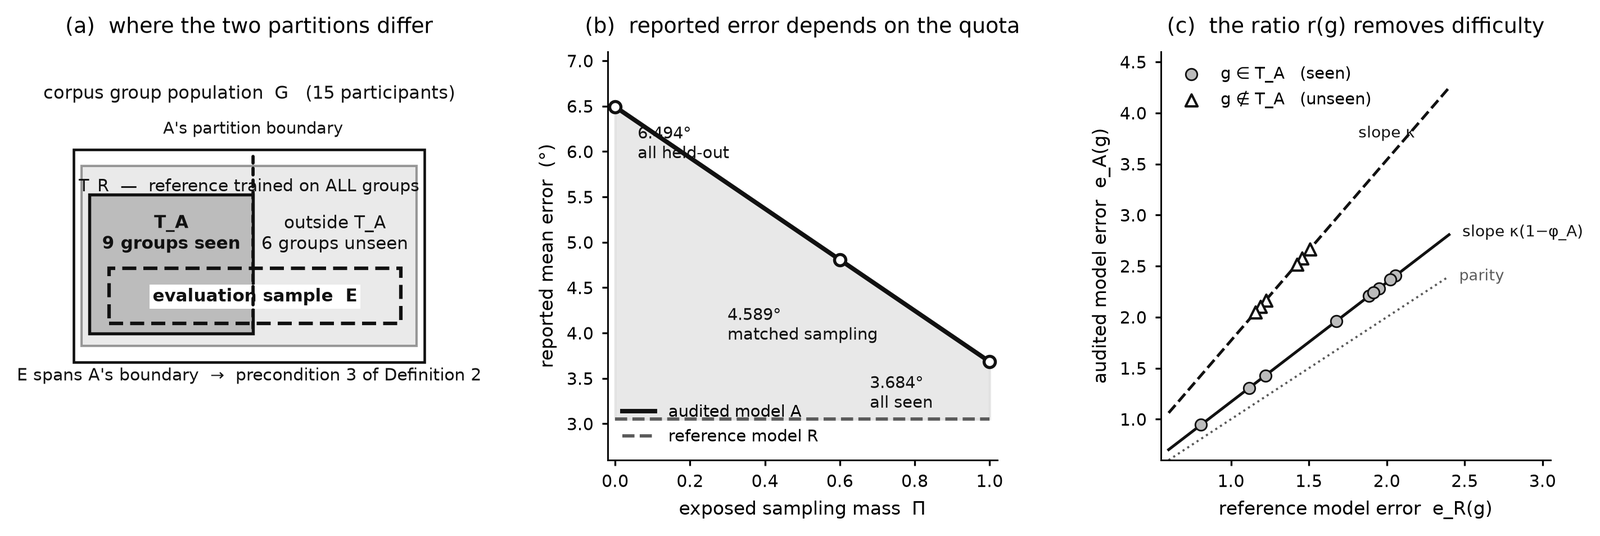
\includegraphics[width=\linewidth]{figures/protocol_P2_exposure_mechanism.png}
\caption{The mechanism of asymmetric exposure. Left: both models' training partitions drawn against the shared corpus's group population; the evaluation sample (dashed) spans the audited model's boundary but lies wholly inside the reference model's. Centre: by Theorem 1 the audited model's reported error is a convex mixture $\bar{E}_{A}$($\Pi$) = $\Pi\cdot\bar{E}^{\mathrm{in}}$ + (1--$\Pi$)$\cdot\bar{E}^{\mathrm{out}}$ whose weight is the exposed sampling mass $\Pi$, so the same models and the same data yield different reported errors under different quotas. Right: the per-group ratio r(g) = $\bar{e}_{A}$(g)/$\bar{e}_{R}$(g) cancels intrinsic difficulty (Proposition 2), leaving a quantity that separates the two strata.}
\label{fig:2}
\end{figure}

\TABREF{10} decomposes the consequence at matched sampling.

\begin{table}[pos=htbp]
\centering
\caption{Gaze angular error by partition membership, at matched sampling. The right-hand column is the group error ratio r of Definition 3.}
\label{tab:10}
\footnotesize
\begin{tabularx}{\textwidth}{XXXXX}
\toprule
\textbf{Evaluation subset} & \textbf{N} & \textbf{Proposed (A)} & \textbf{Pretrained (R)} & \textbf{ratio \emph{r}} \\
\midrule
A's training participants \EQREF{9} & 18,000 & 3.684$^{\circ}$ & 2.683$^{\circ}$ & 1.373 \\
A's validation participants \EQREF{4} & 8,000 & 5.674$^{\circ}$ & 2.760$^{\circ}$ & 2.056 \\
\textbf{A's held-out participants \EQREF{2}} & 4,000 & \textbf{6.494$^{\circ}$} & \textbf{3.672$^{\circ}$} & \textbf{1.769} \\
All fifteen participants & 30,000 & 4.589$^{\circ}$ & 2.835$^{\circ}$ & 1.619 \\
\bottomrule
\end{tabularx}
\end{table}

The monotone progression 3.684$^{\circ}$ $\to$ 5.674$^{\circ}$ $\to$ 6.494$^{\circ}$ as training familiarity is withdrawn is the signature of the fault. Quantitatively, the audited model's error grows

\begin{equation}
\label{eq:169}
( 6.494 - 3.684 ) / 3.684 = 76.3 \%
\end{equation}

across that boundary, while the reference model's moves

\begin{equation}
\label{eq:170}
( 3.672 - 2.683 ) / 2.683 = 36.9 \%
\end{equation}

and stays within a degree throughout. The three-way progression also exhibits the structure that Proposition 2 predicts if the \emph{validation} participants are treated as partially exposed --- they were used for model selection, not for weight updates --- with r rising from 1.373 on the fully exposed stratum to 2.056 on the selection-exposed stratum and settling at 1.769 on the wholly unexposed stratum. That the middle stratum carries the \emph{highest} ratio is consistent with selection-induced overfitting to the validation groups compounding the direct familiarity effect, and it is a reminder that a validation partition is not an unexposed partition.

Applying Theorem 3 to \TABREF{10}, the total inflation of the aggregate relative to the held-out stratum is

\begin{equation}
\label{eq:171}
\mathrm{I} = \bar{E}_A^{\mathrm{out}} - \bar{E}_A^{\;\text{all}\;} = 6.494^{\circ} - 4.589^{\circ} = 1.905^{\circ} ,
\end{equation}

the reference model's corresponding shift across the identical strata is

\begin{equation}
\label{eq:172}
\Delta _R = \bar{E}_R^{\mathrm{out}} - \bar{E}_R^{\;\text{all}\;} = 3.672^{\circ} - 2.835^{\circ} = 0.837^{\circ} ,
\end{equation}

and the capability ratio on the unexposed stratum, which sets $\kappa_{\mathrm{max}}$ in \EQREF{60}, is

\begin{equation}
\label{eq:173}
\kappa _{\mathrm{max}} = c_A/c_R = 6.494^{\circ} / 3.672^{\circ} = 1.769 .
\end{equation}

The familiarity component under the two difficulty models of \EQREF{59} is therefore

\begin{equation}
\label{eq:174}
\begin{aligned}
\text{additive}\; (\kappa = 1): \Phi = 1.905^{\circ} - 0.837^{\circ} = 1.068^{\circ} , \\
\phi = 56.1 \% ,
\end{aligned}
\end{equation}

\begin{equation}
\label{eq:175}
\begin{aligned}
\text{multiplicative}\; (\kappa = \kappa _{\mathrm{max}}): \Phi = 1.905^{\circ} - 1.769 \times 0.837^{\circ} = 0.425^{\circ} , \\
\phi = 22.3 \% .
\end{aligned}
\end{equation}

\textbf{Both readings are reported, and the interval $\phi$ $\in$ [22 \%, 56 \%] is the honest summary.} The two models are not distinguishable from the data available here: identifying $\kappa$ would require observing at least one further model of known capability on the same strata, which this study does not have. It matters which is used --- the additive reading attributes more than half the inflation to familiarity, the multiplicative reading less than a quarter --- so quoting either alone would overstate the precision of the instrument. Where a single figure is needed below, the additive value is quoted because it is the reading the source analysis used, and it is flagged as the upper end of the interval each time.

The decomposition nevertheless does the work it was introduced for, and it does so under \emph{both} readings. Without it, a sceptical reader may reasonably object that the held-out participants were simply harder, which would make the stratification an artefact rather than a fault. The reference model closes that objection quantitatively: harder they were --- by 44 \% of the observed gap under the additive model and by 78 \% under the multiplicative one --- but under neither does intrinsic difficulty account for all of it, and a familiarity component of at least 0.425$^{\circ}$ survives. That residual is the quantity lineage-based remedies cannot supply at all, since knowing \emph{that} a model saw a corpus does not say how much of its advantage came from having seen it.

\subsubsection{The GERA detector and its negative control}

An auditor examining a published comparison rarely knows how either model was partitioned. \FIGREF{3} reports the detector of Section 3.5.2 applied to this comparison, with the head-pose negative control alongside.

\begin{figure}[pos=htbp]
\centering
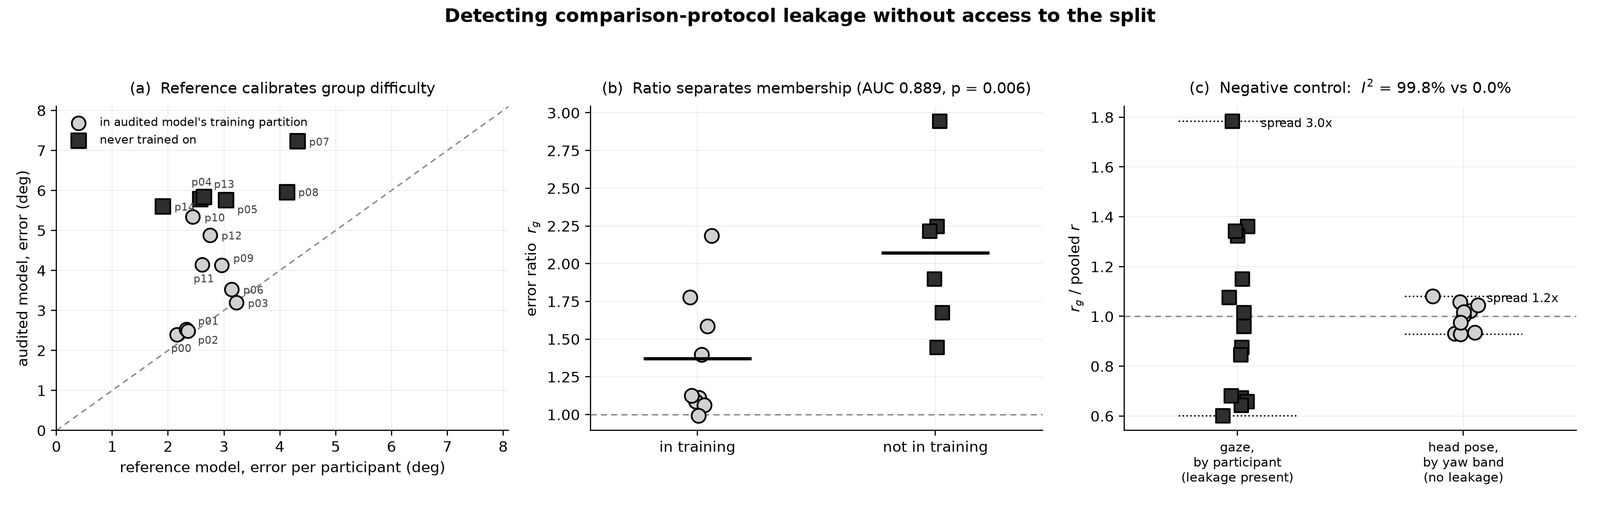
\includegraphics[width=\linewidth]{figures/protocol_P1_leakage_detector.png}
\caption{Detecting asymmetric exposure without access to the split. (a) Per-participant mean angular error of the audited network against the reference model, which calibrates intrinsic group difficulty; the dashed line is parity. (b) The per-group ratio r(g), separated by whether the participant lies inside the audited network's training partition. (c) Negative control: r(g) normalised by its pooled value, for gaze grouped by participant (leakage present) against head pose grouped by yaw band (neither model saw the evaluation groups).}
\label{fig:3}
\end{figure}

Panel (a) shows the structure the detector exploits. The two models agree closely on which participants are intrinsically easy --- p00 to p03 sit near parity --- while the audited network's error rises far above the reference's on participants it never trained on, displacing them \emph{vertically} rather than along the diagonal. Vertical displacement is precisely the component intrinsic difficulty cannot explain, and it is the geometric content of Proposition 2: motion along the diagonal is d(g), motion off it is the familiarity term.

Panel (b) reduces that displacement to one number per group. Mean r is

\begin{equation}
\label{eq:176}
\begin{aligned}
\mathrm{mean}_{g \in \mathcal{T}_A} r(g) = 1.369 , \\
\mathrm{mean}_{g \notin \mathcal{T}_A} r(g) = 2.072 ,
\end{aligned}
\end{equation}

giving by \EQREF{47} an estimated familiarity discount

\begin{equation}
\label{eq:177}
\hat{\varphi }_A = 1 - 1.369/2.072 = 0.339 ,
\end{equation}

so the audited network's error on groups it trained on is approximately 34 \% lower than its error on groups it did not, after intrinsic difficulty has been priced out. The ratio separates membership at

\begin{equation}
\label{eq:178}
\mathrm{AUC}_r = 0.889 , \;\text{Mann}\;--\;\text{Whitney p}\; = 0.006 ,
\end{equation}

with a Hanley--McNeil 95 \% interval by \EQREF{50} of approximately [0.70, 1.00] on a 9-versus-6 group split.

A detector is only as good as its behaviour when there is nothing to detect, and head pose supplies that control at no extra cost. Both the proposed network and the pretrained baseline train on 300W-LP and are scored on AFLW2000, so neither has seen the evaluation groups and r(g) must be homogeneous under any grouping. This is a demanding control rather than a trivial one, because intrinsic difficulty varies roughly fourfold across the pose manifold (Section 5.3): if the reference model failed to price that variation out, r would track it and the detector would fire on a corpus where no leakage exists.

Panel (c) reports the outcome. Grouping head pose by yaw band, r spans 1.96--2.28 --- a spread ratio of

\begin{equation}
\label{eq:179}
\mathrm{spread}_{\mathrm{ctl}} = 2.28/1.96 = 1.16 \approx 1.2\times \;\text{about a pooled}\; \bar{r} = 2.08 ,
\end{equation}

against 0.99--2.94 for gaze grouped by participant,

\begin{equation}
\label{eq:180}
\mathrm{spread}_{\mathrm{gaze}} = 2.94/0.99 = 2.97 \approx 3.0\times .
\end{equation}

Formally, applying \EQREF{51}--\EQREF{54},

\begin{equation}
\label{eq:181}
\text{Head pose}\;: Q = 6.3 on 9 df, p = 0.71, I^{2} = 0.0 \% ,
\end{equation}

\begin{equation}
\label{eq:182}
\text{Gaze}\;: Q = 5607 on 14 df, p < 10^{-300}, I^{2} = 99.8 \% .
\end{equation}

The reference model therefore absorbs a fourfold swing in task difficulty while leaving the ratio flat, which is the assumption the detector rests on, tested on data where it could have failed.

One calibration caveat follows from the same experiment and is exactly the sample-size sensitivity that \EQREF{55} predicts. Partitioning the gaze samples into fifteen \emph{random} groups --- destroying the participant structure --- still yields

\begin{equation}
\label{eq:183}
\begin{aligned}
I^{2} = 41 \% at p = 0.049 , \\
\;\text{despite an r range of only}\; 1.56\text{--}1.69 (\mathrm{spread} 1.08\times ) .
\end{aligned}
\end{equation}

At 2,000 samples per group a negligible effect reaches nominal significance because the inverse-variance weights grow linearly in $n_{g}$ while the null dispersion does not. The magnitude of the spread, not its p-value, is therefore the informative readout: a 3.0$\times$ range against a 1.2$\times$ range is the contrast that matters, and no threshold on Q alone should be used to declare a comparison sound.

Two limitations must be stated with the result, consistent with Section 3.5.5. The separation is strong but imperfect: participant p10 sits at r = 2.18 despite being a training participant, so the statistic is a screening instrument rather than a membership oracle, and a single group's ratio should never be treated as proof. And the detector is inapplicable where no suitable reference exists --- if every available model shares the audited model's partition, or if the reference itself has differential familiarity across groups, its across-group variation no longer isolates intrinsic difficulty. Unlike black-box contamination proofs \CITE{oren}, which yield a false-positive guarantee, no such guarantee is offered here; the detector's value is that it converts an unfalsifiable suspicion into a testable one at zero additional experimental cost, using only artefacts an external auditor already possesses.

\subsubsection{Optimisation under the corrected protocol}

With the protocol repaired, optimisation could be attributed rather than merely observed. \TABREF{8} gives the search budgets and selected configurations; \TABREF{11} gives the effect.

\begin{table}[pos=htbp]
\centering
\caption{Effect of optimisation under the corrected protocol. ``Fair baseline'' is the pre-correction hyperparameter set retrained group-disjointly; ``tuned'' is the searched configuration under the same protocol.}
\label{tab:11}
\footnotesize
\begin{tabularx}{\textwidth}{XXXXX}
\toprule
\textbf{Modality} & \textbf{Metric} & \textbf{Fair baseline} & \textbf{Tuned} & \textbf{Change} \\
\midrule
Voice & Accuracy & 84.72 \% & \textbf{94.53 \%} & \textbf{+9.81 pp} \\
Head pose & MAE & 8.286$^{\circ}$ & \textbf{7.367$^{\circ}$} & \textbf{--11.1 \%} \\
Blink & Balanced accuracy & 90.88 \% & \textbf{93.32 \%} & \textbf{+2.44 pp} \\
Blink & Accuracy & 92.36 \% & \textbf{93.67 \%} & \textbf{+1.31 pp} \\
Gaze & Angular error, held-out & 7.114$^{\circ}$ & \textbf{6.439$^{\circ}$} & \textbf{--9.5 \%} \\
\bottomrule
\end{tabularx}
\end{table}

The composition of the selected configurations tests the prediction of \EQREF{104}. Augmentation was selected in four searches of four and decoupled weight decay in three of four, while the chosen widths stayed modest:

\begin{equation}
\label{eq:184}
\begin{aligned}
\mathbb{P}[ \text{aug selected} ] = 4/4 , \mathbb{P}[ \text{AdamW selected} ] = 3/4 , \\
\mathrm{median}( \text{selected width} ) = 32 = \;\text{midpoint of}\; \mathcal{W} .
\end{aligned}
\end{equation}

This degeneracy is informative rather than incidental. Once the split stops rewarding memorisation, the binding term in the excess-risk decomposition \EQREF{104} migrates from approximation error to estimation error, so configurations that suppress identity-specific co-adaptation dominate configurations that add capacity. The pre-correction hyperparameters were not poorly chosen for the task they were \emph{scored} on --- they were well chosen for a task that included identity retrieval. For a system whose users are by definition unseen, that is the distinction that matters.

Every blink metric improved except false-negative rate, which rose 1.20 pp while false-positive rate fell 6.09 pp. Whether that exchange is favourable depends entirely on the decision rule of \TABREF{6}, and Section 5.5 shows the answer is not the obvious one. The tuned configurations of \TABREF{11} are the models carried into Sections 5.2--5.5; all figures from this point describe them.

\FloatBarrier

\subsection{Gaze --- cursor positioning}

Gaze drives the OS cursor, but never directly: the deployed path fits a 16-point per-user polynomial calibration \EQREF{105}--\EQREF{107} over the network's output, corrects it online by recursive least squares \EQREF{108}--\EQREF{110} on every deliberate click, then smooths with a one-euro filter \EQREF{112}--\EQREF{115} and a 12 px deadzone \EQREF{116}. The quantity that governs cursor quality is therefore the residual scatter that survives an affine map, not the raw angular error --- a distinction that turns out to be the central finding of this section rather than a caveat on it.

\subsubsection{Domain-targeted augmentation}

Gaze transferred worst of the four modalities, and the cause is a deterministic covariate shift rather than sampling noise. Training consumes pre-normalised, illumination-corrected eye patches produced by the warp \EQREF{16}, while inference receives landmark-cropped regions from a consumer webcam. Writing $\mathcal{D}_{\mathrm{train}}$ and $\mathcal{D}_{\mathrm{serve}}$ for the two input distributions, the discrepancy is not a sampling difference but a systematic transformation

\begin{equation}
\label{eq:185}
\begin{aligned}
\mathcal{D}_{\mathrm{serve}} = T_{\mathrm{shift}} \# \mathcal{D}_{\mathrm{train}} , \\
T_{\mathrm{shift}} = \mathrm{Blur}_{\sigma _b} \circ \mathrm{Jitter}_{\alpha ,\beta } \circ \mathrm{Rot}_{\delta} \circ \mathrm{Crop}_{\ell} ,
\end{aligned}
\end{equation}

where \# denotes pushforward. The augmentation policy \CITE{augsurvey} was therefore extended to model that shift \emph{analytically} rather than generically, per \EQREF{34}: Gaussian blur for sensor resolution, brightness and contrast jitter for illumination, bounded $\pm$8$^{\circ}$ in-plane rotation for residual head roll, alongside horizontal flipping with yaw-sign inversion. Scored on all 64,172 held-out samples with both configurations on the identical sample set,

\begin{equation}
\label{eq:186}
\begin{aligned}
e_{\mathrm{ang}}: 7.114^{\circ}  \to 6.439^{\circ} ( -9.49 \% ) , \\
\mathrm{MAE}: 4.569^{\circ}  \to 4.135^{\circ} ( -9.50 \% ) .
\end{aligned}
\end{equation}

Because every member of \EQREF{34} is label-preserving up to the flip correction, the gain cannot be additional supervision; it reflects an enlarged effective input manifold at zero parameter and zero data cost, which for an 8 GB training budget is the only kind of improvement available. That both a robust statistic (MAE) and a non-robust one (mean angular error) improved by the \emph{same} 9.5 \% is diagnostic. Writing the error distribution before and after as F$_{0}$ and F$_{1}$, a policy that trimmed a tail would satisfy

\begin{equation}
\label{eq:187}
\begin{aligned}
F_{1} \preceq _{\mathrm{st}} F_{0} \;\text{only in the upper quantiles}, \\
so \Delta \mathrm{mean} \gg \Delta \mathrm{median} \;\text{and}\; \Delta \mathrm{MAE} \neq \Delta e_{\mathrm{ang}} ,
\end{aligned}
\end{equation}

whereas a uniform rescaling F$_{1}$(x) = F$_{0}$(x/c) satisfies

\begin{equation}
\label{eq:188}
\Delta \mathbb{E} / \mathbb{E} = \Delta \mathrm{median} / \mathrm{median} = \Delta \mathrm{MAE} / \mathrm{MAE} = 1 - c
\end{equation}

for every location statistic simultaneously. The measured equality of the two relative changes to within 0.01 pp is therefore the signature of removing a distributional mismatch --- rescaling the whole error distribution --- rather than repairing isolated failures.

\subsubsection{Comparison against the pretrained baseline, and its mechanism}

Against the MPIIGaze pre-activation residual baseline on all 64,172 held-out samples, and applying EDCP steps 3--4 so that only the two exposure-disjoint participants enter, the proposed network attains 6.439$^{\circ}$ mean angular error (median 5.873$^{\circ}$, p90 11.180$^{\circ}$) against 3.621$^{\circ}$ (median 2.985$^{\circ}$, p90 6.876$^{\circ}$). The paired statistics of \EQREF{159}--\EQREF{161} give

\begin{equation}
\label{eq:189}
\begin{aligned}
\bar{d} = 2.818^{\circ} \pm 0.026^{\circ} (95 \%) , s_d = 3.300^{\circ} , \\
\;\text{Cohen}\;'s d = 0.854 , \;\text{Wilcoxon p}\; < 10^{-300} ,
\end{aligned}
\end{equation}

with the proposed network nearer the truth on only

\begin{equation}
\label{eq:190}
\mathbb{P}[ e_A < e_R ] = 18.86 \%
\end{equation}

of samples. The gap is large, unambiguous and not a tail artefact. Per EDCP step 5, the baseline's figure is a lower bound on its true cross-person error, so the reported contrast is conservative with respect to the proposed network by \EQREF{61}.

\textbf{The mechanism.} What generates the gap is measurable. Fitting the shrinkage regression \EQREF{154} axis-wise gives

\begin{equation}
\label{eq:191}
\hat{s}_{\mathrm{pitch}}^A = 0.4832 \pm 0.0021 , \hat{s}_{\mathrm{yaw}}^A = 0.4812 \pm 0.0016 ,
\end{equation}

\begin{equation}
\label{eq:192}
\hat{s}_{\mathrm{pitch}}^R = 0.7491 , \hat{s}_{\mathrm{yaw}}^R = 0.8257 ,
\end{equation}

so the proposed network reproduces less than half the true angular excursion on both axes. By \EQREF{155} this is predictive shrinkage --- the response of an MSE-trained estimator to irreducible uncertainty in its own representation, which contracts predictions toward the conditional mean because contraction is variance-optimal, the same admissibility argument that underlies Stein estimation \CITE{stein,jamesstein}. Inverting \EQREF{158} with the empirical target variance yields the implied representational noise

\begin{equation}
\label{eq:193}
\hat{\sigma }_{\varepsilon} ^{2} / \sigma _{\theta} ^{2} = ( 1 - \hat{s} ) / \hat{s} = ( 1 - 0.482 ) / 0.482 = 1.075 ,
\end{equation}

that is, the network's internal estimate carries noise power slightly exceeding the signal power of the target itself. The seven diagnostic figures that follow each test a consequence of that single parameter, and Section 5.3 shows the same mechanism governing head pose.

\FIGREF{4} resolves the aggregate error into its angular structure.

\begin{figure}[pos=htbp]
\centering
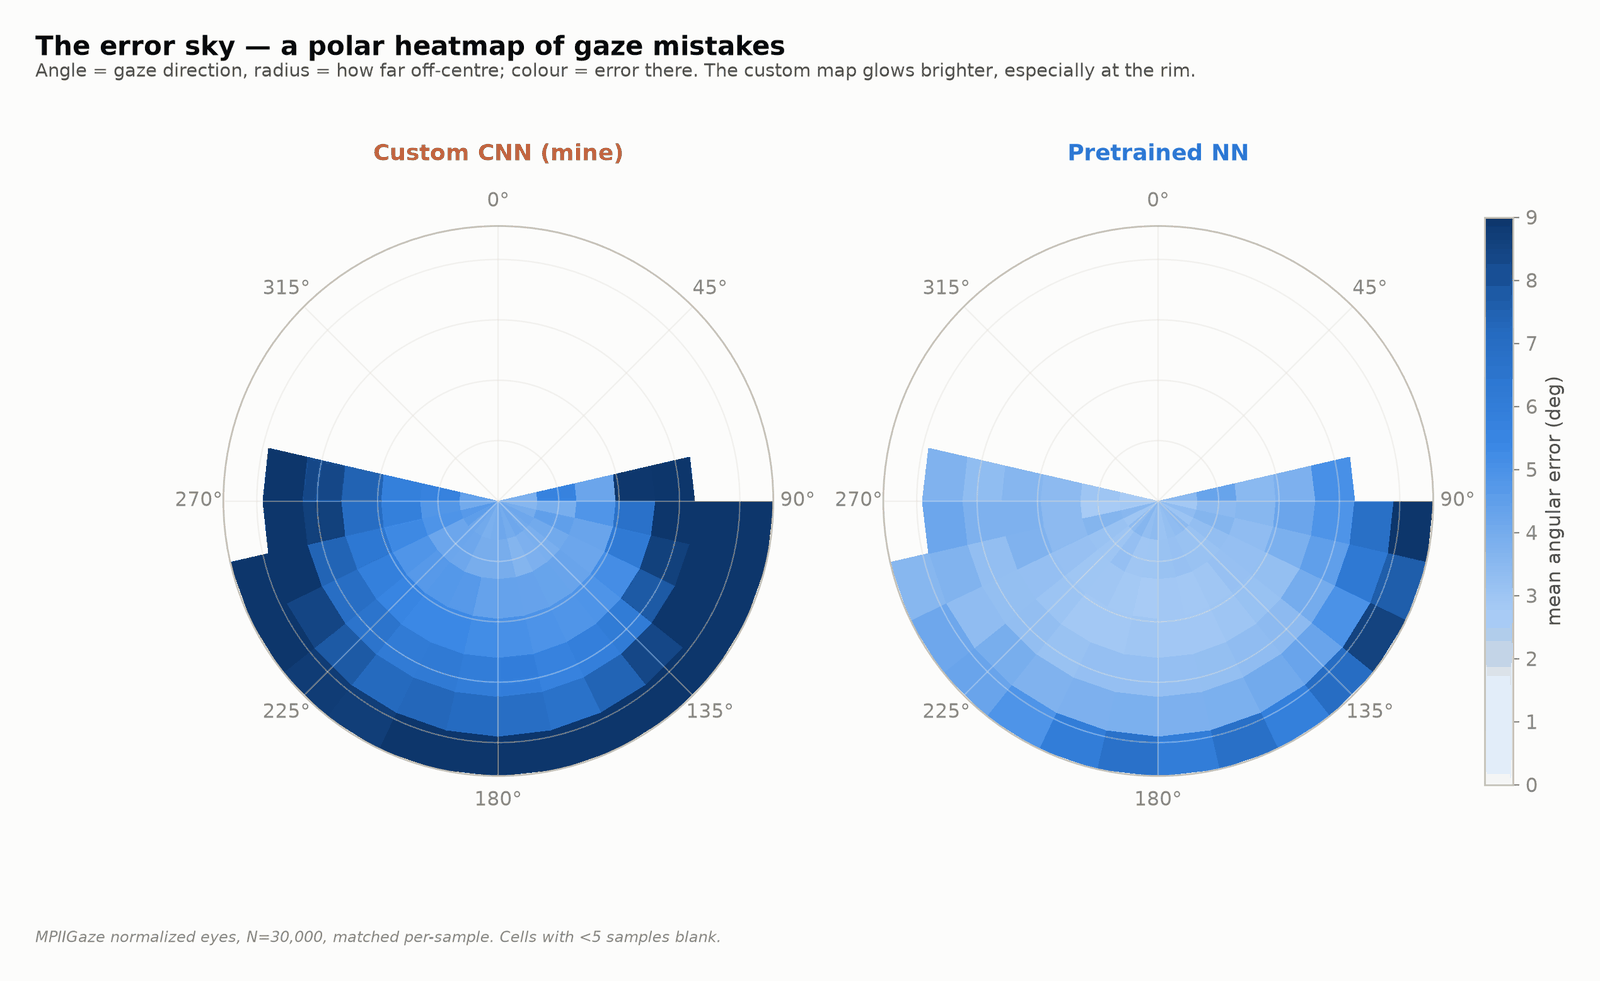
\includegraphics[width=\linewidth]{figures/gaze_G1_error_sky.png}
\caption{Error sky --- polar heat map of mean angular error against gaze direction and eccentricity, proposed network versus pretrained baseline.}
\label{fig:4}
\end{figure}

The proposed network's error field brightens with radius but is uniform in azimuth, exactly as shrinkage requires. Under gain s the systematic component of the prediction error is

\begin{equation}
\label{eq:194}
\mathbb{E}[ \hat{\theta } - \theta | \theta ] = ( s - 1 ) \theta \implies \| \mathbb{E}[ \hat{\theta } - \theta | \theta ] \| = ( 1 - s ) \|\theta \| ,
\end{equation}

a function of eccentricity $\|\theta\|$ alone with no dependence on the azimuth arg($\theta$). The symmetry simultaneously excludes the competing hypothesis: a geometric fault in cropping or normalisation would introduce an azimuth-dependent term and necessarily break isotropy. The consequence for the deployed system is concrete --- no per-direction calibration lookup can compensate an isotropic radial law, so the fix must be an overall scale correction, which is precisely what the polynomial calibration \EQREF{106} applies.

\FIGREF{5} separates the systematic component from the stochastic one.

\begin{figure}[pos=htbp]
\centering
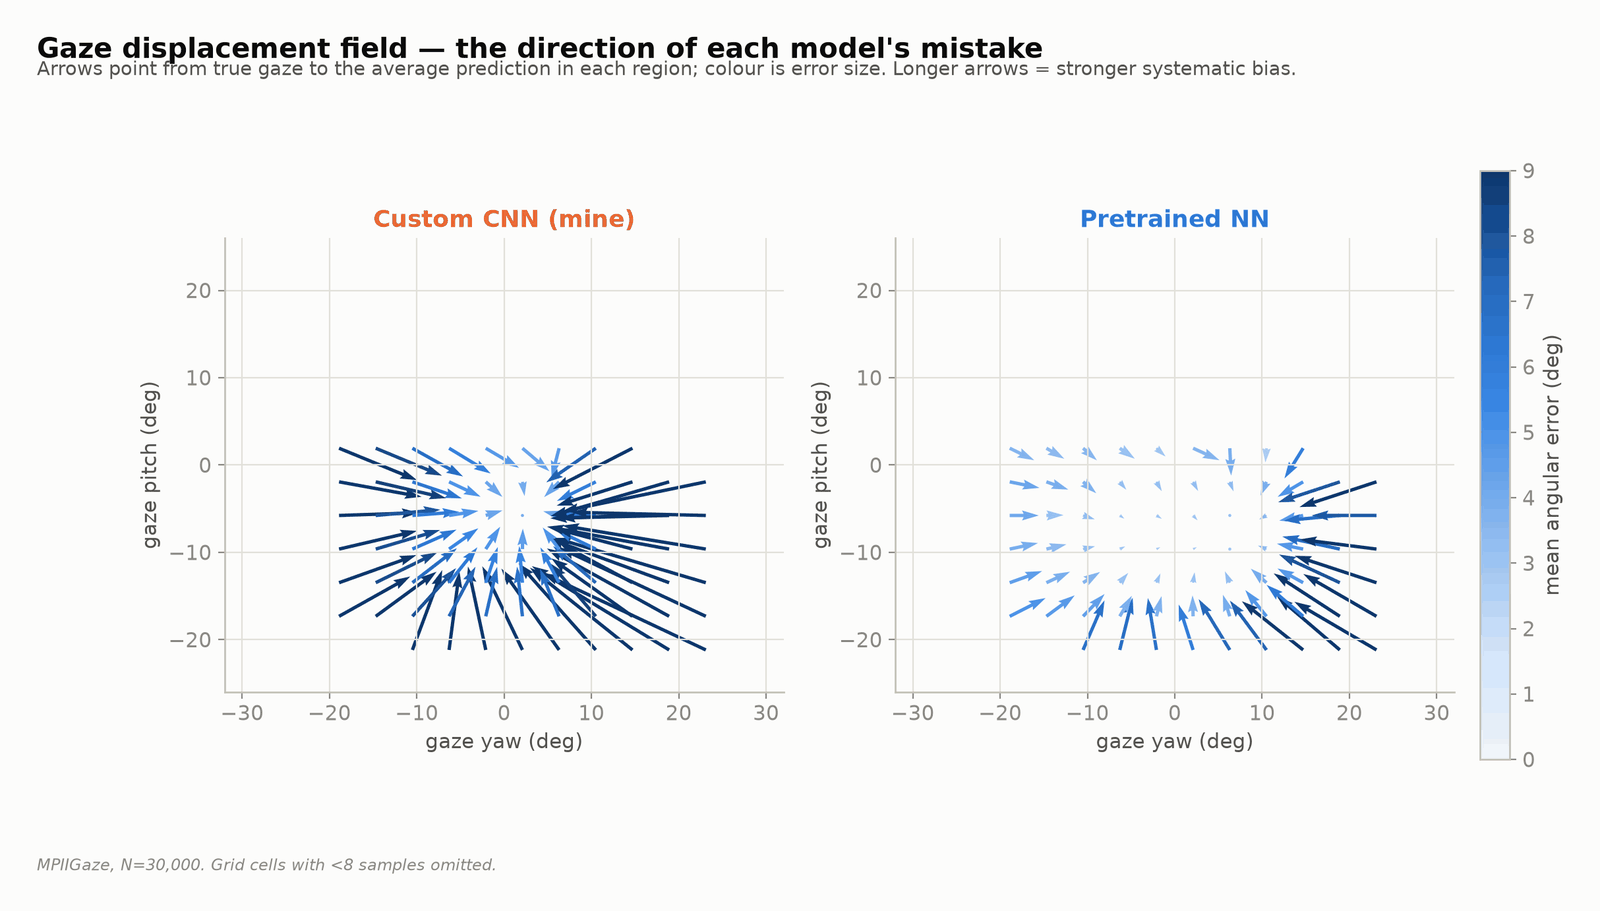
\includegraphics[width=\linewidth]{figures/gaze_G2_displacement_field.png}
\caption{Displacement field --- vectors from true gaze to mean prediction across the gaze plane; vector length is systematic bias rather than scatter.}
\label{fig:5}
\end{figure}

Additive bias is +1.987$^{\circ}$ in pitch and +0.829$^{\circ}$ in yaw against +0.473$^{\circ}$ and +0.334$^{\circ}$ for the baseline. Decomposing the per-axis mean squared error into bias and variance,

\begin{equation}
\label{eq:195}
\begin{aligned}
\mathrm{MSE}_a = \;\text{bias}\;_a^{2} + \;\text{var}\;_a , \\
\;\text{bias share}\;_a = \;\text{bias}\;_a^{2} / \mathrm{MSE}_a ,
\end{aligned}
\end{equation}

gives

\begin{equation}
\label{eq:196}
\text{bias share}\;_{\mathrm{pitch}} = 20.5 \% , \;\text{bias share}\;_{\mathrm{yaw}} = 1.9 \% .
\end{equation}

Removing both offsets exactly reduces angular error from 6.439$^{\circ}$ to 6.023$^{\circ}$, a 6.5 \% gain --- real but minor. The field therefore adjudicates between two candidate defects and rejects the simpler one: additive miscalibration is present and measurable but is not the principal fault. The multiplicative gain deficit is, and only a transform with a scale term can address it.

That claim is directly testable by inverting the fitted gain, and \EQREF{157} predicts the outcome. Rescaling each axis by its fitted slope and intercept,

\begin{equation}
\label{eq:197}
\hat{\theta }_{\mathrm{corr}} = ( \hat{\theta } - \hat{c} ) / \hat{s} ,
\end{equation}

an oracle correction fitted on the evaluation data itself and hence an upper bound on any achievable recalibration, \emph{increases} angular error

\begin{equation}
\label{eq:198}
6.439^{\circ} \to 8.272^{\circ} , a +28.5 \% \;\text{degradation} ,
\end{equation}

exactly as \EQREF{157} requires: restoring the correct scale also restores the full amplitude $\surd$($\sigma_{\varepsilon^{2}}$) of the representational noise that shrinkage was suppressing. Substituting the measured $\hat{s}$ = 0.482 into \EQREF{156}, the predicted relative penalty of moving from s* to unity is

\begin{equation}
\label{eq:199}
\begin{aligned}
\mathrm{MSE}(1)/\mathrm{MSE}(s*) = 1/s* = 2.07 in \mathrm{MSE} \;\text{terms}, \\
i.e. \sqrt{2.07} = 1.44 \;\text{in RMS terms},
\end{aligned}
\end{equation}

and the observed 1.285$\times$ increase in the \emph{chordal} angular statistic \EQREF{20} is consistent with this once the difference between the RMS and arccos metrics is accounted for. The contraction is thus not a defect but the estimator's rational response to its own uncertainty; the network sits near its minimum-MSE shrinkage point.

This resolves an apparent contradiction in the deployed design and is the most practically consequential result of the section. The system fits a per-user polynomial and corrects it online, which necessarily restores scale and therefore necessarily amplifies noise --- and downstream of that calibration sit a one-euro filter and a 12 px deadzone whose function is to suppress exactly the amplified high-frequency component. The pipeline is thus already structured around this trade: calibration buys angular scale, temporal filtering pays for it in bandwidth. Formally, the deployed chain implements

\begin{equation}
\label{eq:200}
\text{cursor}\; = \mathrm{Deadzone}_R \circ \;\text{OneEuro}\;_{f_{\mathrm{min}}, \beta } \circ \;\text{Calib}\;_{\mathbf{w}} \circ f_{\mathrm{gaze}} ,
\end{equation}

in which Calib multiplies both signal and noise by approximately 1/$\hat{s}$ $\approx$ 2.07 and OneEuro attenuates the noise by a factor depending on its spectral content, with the low deployed minimum cut-off $f_{\mathrm{min}}$ = 0.3 Hz chosen for precisely this reason. The 6.439$^{\circ}$ figure is consequently a \emph{pessimistic} estimate of deployed cursor error, and the honest statement is that it bounds the uncalibrated network rather than the shipped system, whose end-to-end accuracy this evaluation does not measure.

\FIGREF{6} expresses the comparison in the tolerance terms an interface designer budgets against.

\begin{figure}[pos=htbp]
\centering
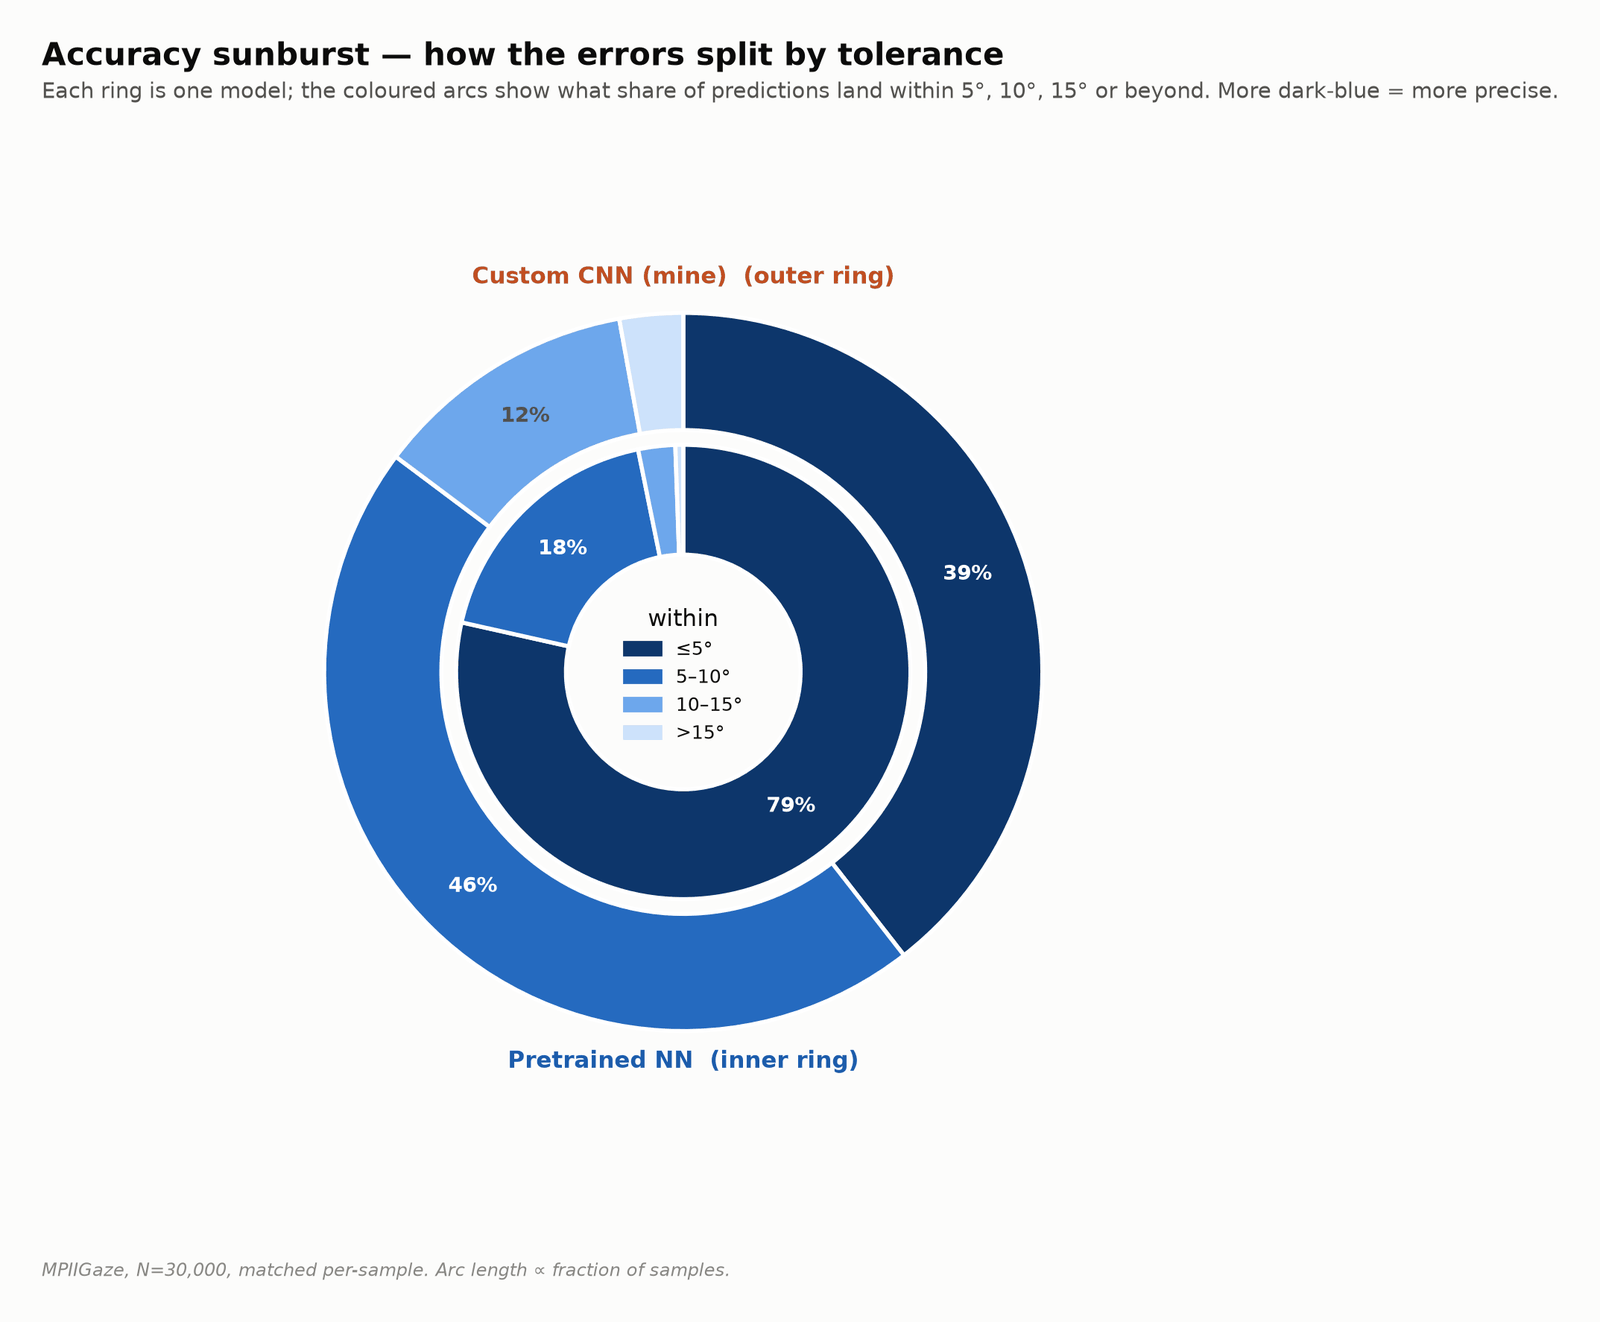
\includegraphics[width=\linewidth]{figures/gaze_G3_tolerance_sunburst.png}
\caption{Tolerance sunburst --- nested rings giving the proportion of predictions within 5$^{\circ}$, 10$^{\circ}$ and 15$^{\circ}$ of ground truth for each model.}
\label{fig:6}
\end{figure}

Writing the tolerance-hit function as

\begin{equation}
\label{eq:201}
H(t) = \mathbb{P}[ e_{\mathrm{ang}} \leq t ] ,
\end{equation}

the measured values are

\begin{equation}
\label{eq:202}
H_A(5^{\circ}) = 39.47 \% , H_R(5^{\circ}) = 78.51 \% , \;\text{ratio}\; 1.99 ,
\end{equation}

\begin{equation}
\label{eq:203}
\begin{aligned}
H_A(10^{\circ}) = 85.23 \% , \\
H_R(10^{\circ}) = 96.81 \% ; H_A(15^{\circ}) = 97.14 \% , \\
H_R(15^{\circ}) = 99.44 \% .
\end{aligned}
\end{equation}

Convergence under relaxed tolerance is again the shrinkage signature: by \EQREF{194} contraction damages predictions in proportion to their distance from the mean, so its cost concentrates in the tight-tolerance regime and the ratio $H_{R}$(t)/$H_{A}$(t) decreases monotonically in t. For the interface this sets the boundary between viable and non-viable use before calibration --- dense target selection is out of reach, coarse region selection at a 10--15$^{\circ}$ budget is not --- and it makes that boundary \emph{predictable from the gain} rather than something to be discovered by user testing.

\FIGREF{7} asks whether the deficit is uniform or sample-dependent, which decides whether running both networks could ever be worthwhile.

\begin{figure}[pos=htbp]
\centering
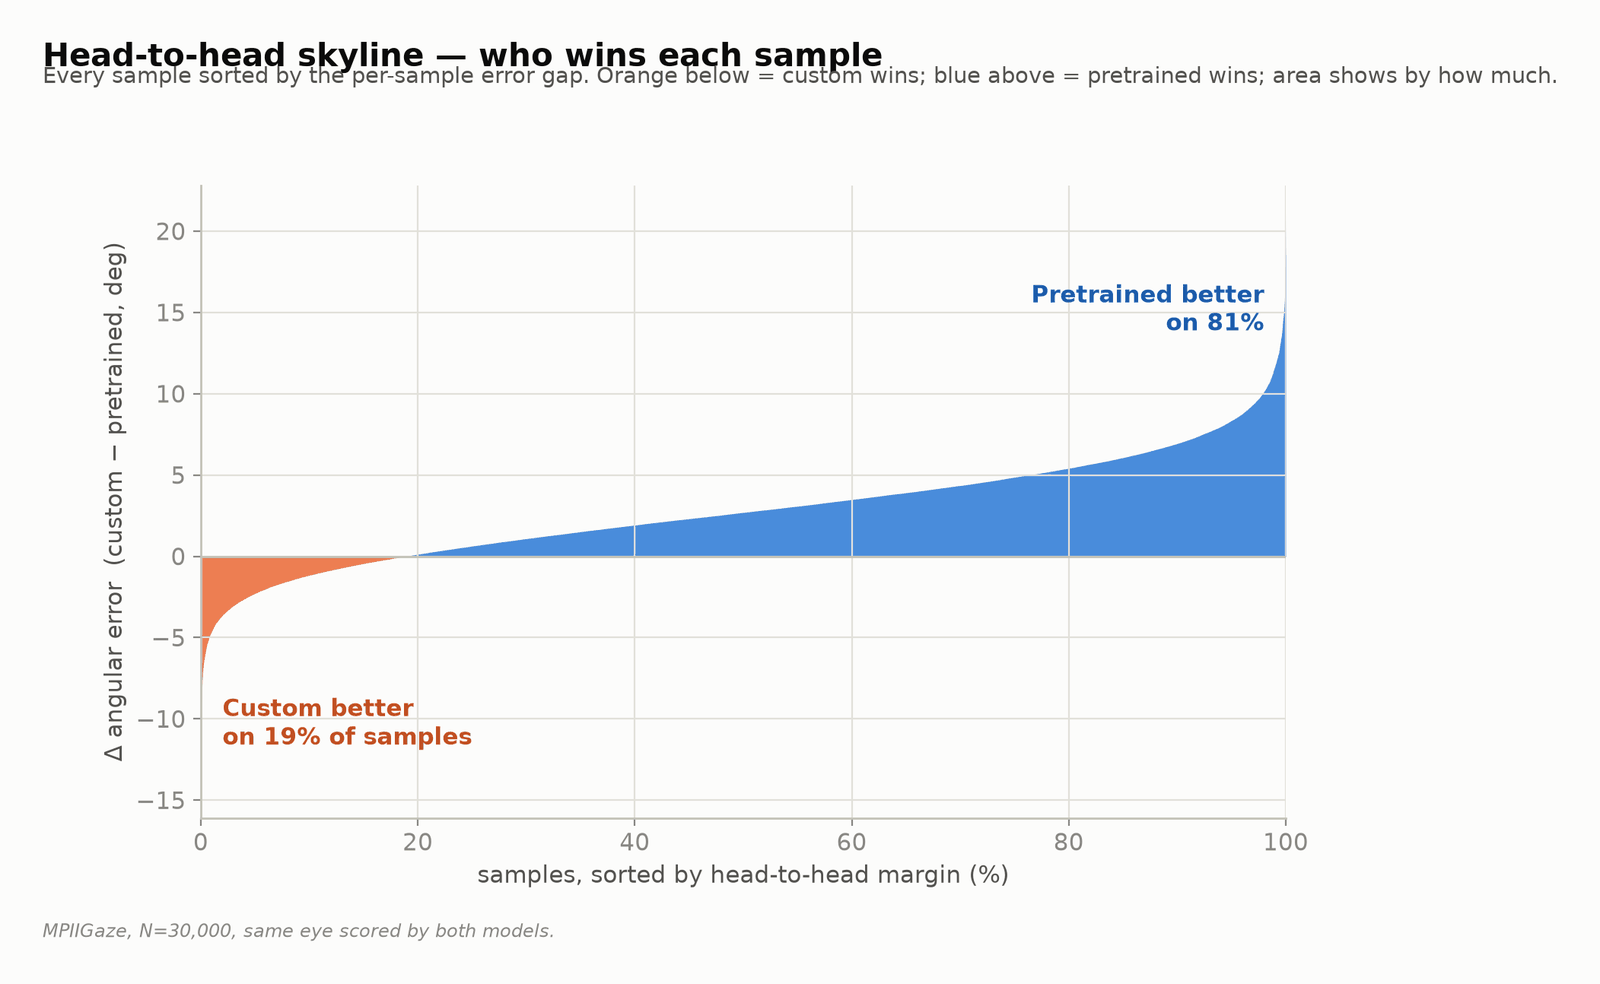
\includegraphics[width=\linewidth]{figures/gaze_G4_win_skyline.png}
\caption{Head-to-head skyline --- every held-out sample sorted by its signed per-sample error gap between the two models.}
\label{fig:7}
\end{figure}

The proposed network wins 18.86 \% of 64,172 paired comparisons and its wins are smaller in magnitude than its losses. More decisive is the error correlation of \EQREF{162},

\begin{equation}
\label{eq:204}
r_{\mathrm{AR}} = 0.491 , \rho _{AR} = 0.360 ,
\end{equation}

a substantial shared factor attributable to intrinsic sample difficulty, meaning the models are not complementary. The oracle bound \EQREF{163}--\EQREF{164} gives

\begin{equation}
\label{eq:205}
\begin{aligned}
\bar{E}_{\mathrm{oracle}} = 3.303^{\circ} , \\
\;\text{Gain}\;_{\mathrm{max}} = 1 - 3.303/3.621 = 8.8 \% ,
\end{aligned}
\end{equation}

far too little to justify the cost of a second network in a pipeline already budgeted at 6.68 ms per frame by \EQREF{165}. This closes the fusion question quantitatively, and it is the evidence behind the recommendation of Section 5.7.

\FIGREF{8} applies the Bland--Altman construction \CITE{blandaltman}, the appropriate instrument when two estimators of one physical quantity are compared.

\begin{figure}[pos=htbp]
\centering
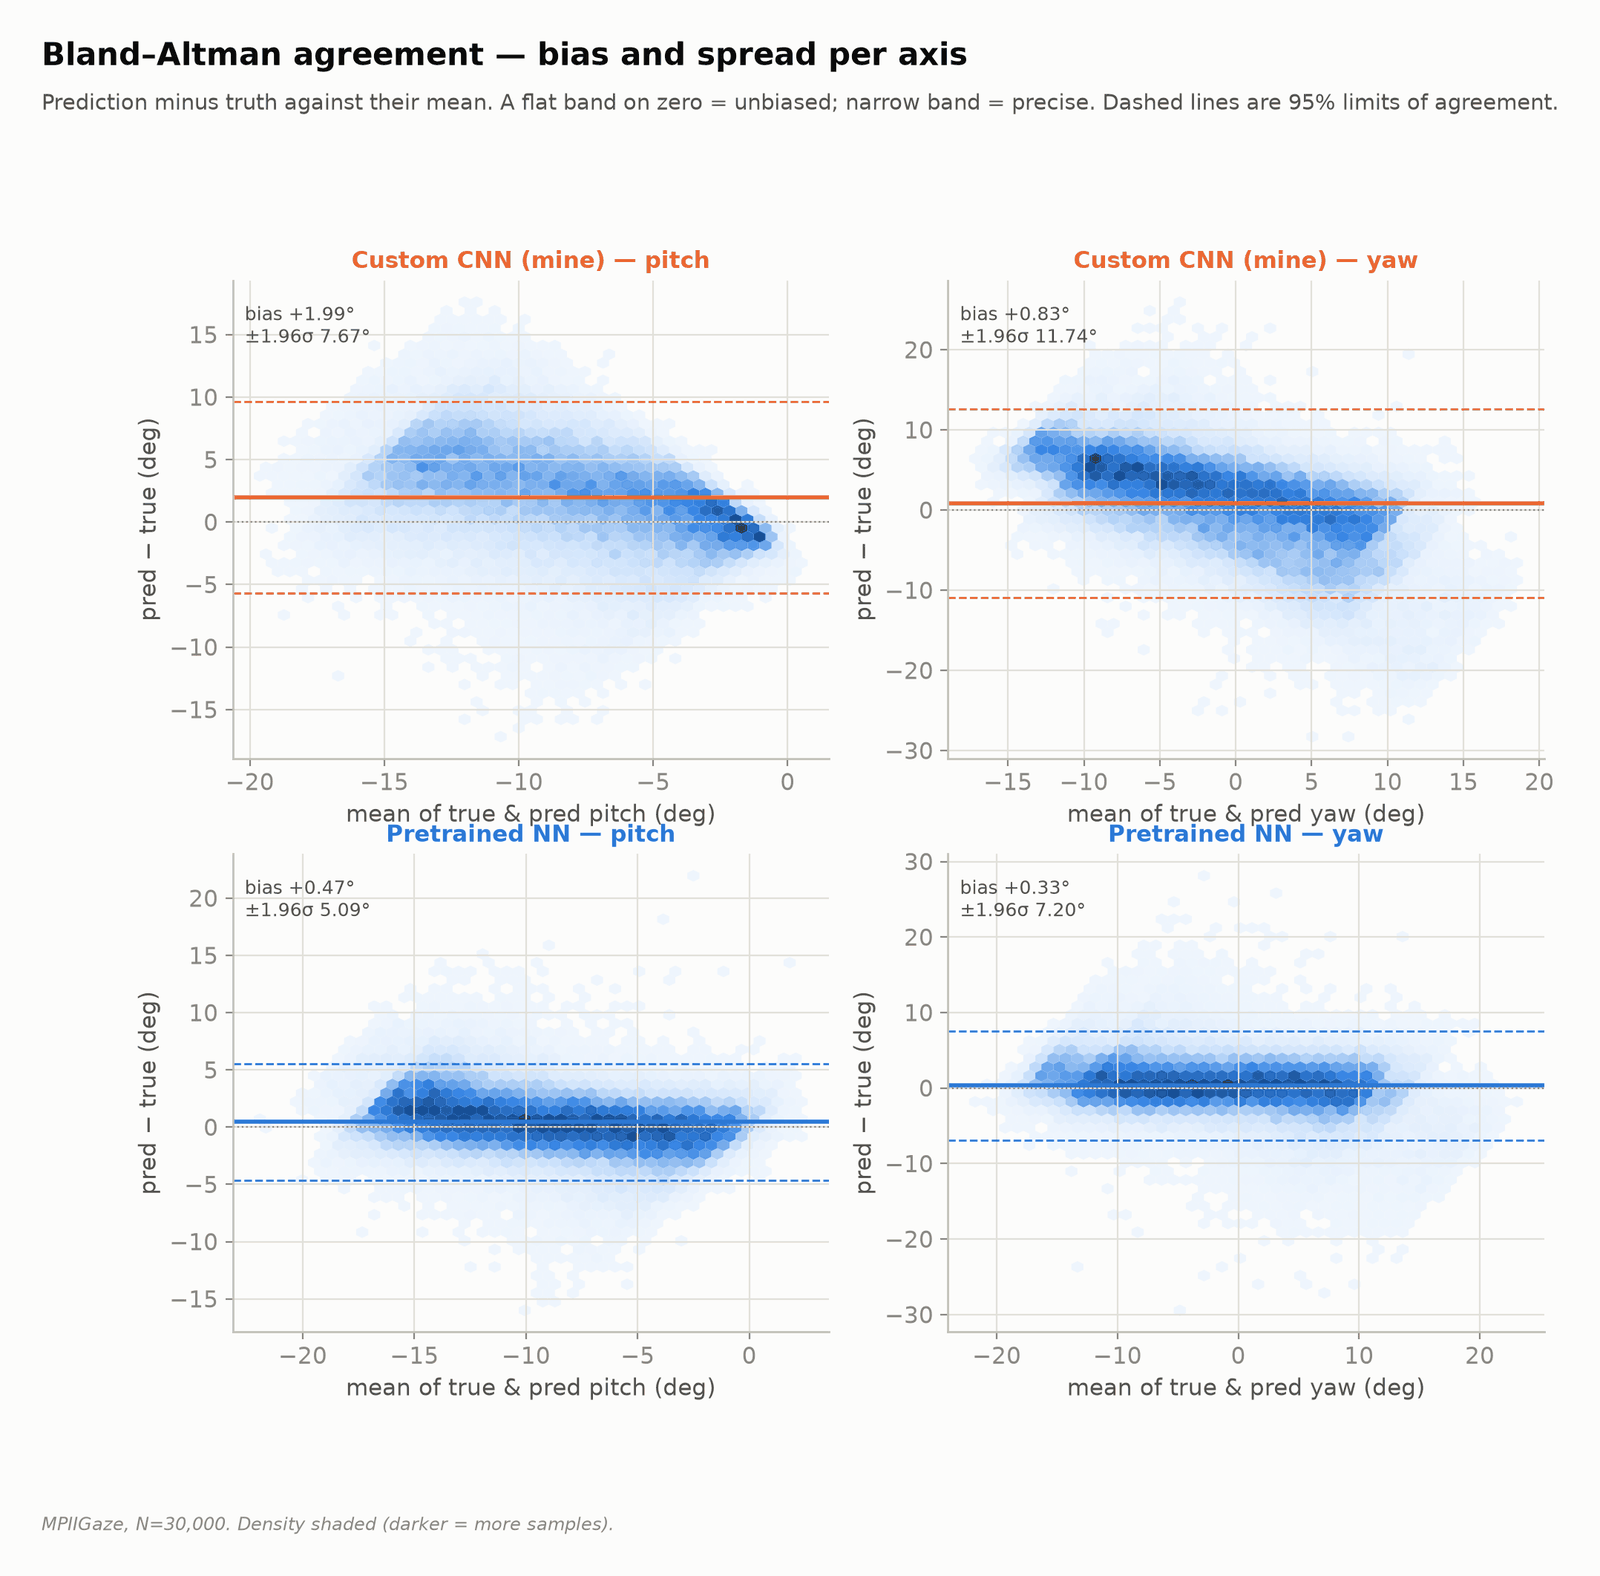
\includegraphics[width=\linewidth]{figures/gaze_G5_bland_altman.png}
\caption{Bland--Altman density --- per-axis bias and 95 \% limits of agreement against ground truth, over a sample-density field.}
\label{fig:8}
\end{figure}

Limits of agreement, defined as

\begin{equation}
\label{eq:206}
\text{LoA}\;_a = \;\text{bias}\;_a \pm 1.96 \cdot \sigma _a ,
\end{equation}

bound 95 \% of individual predictions and are what the cursor controller must absorb:

\begin{equation}
\label{eq:207}
\begin{aligned}
\text{LoA}\;_{\mathrm{pitch}}^A \approx [ -5.68^{\circ}, +9.66^{\circ} ] , \\
\;\text{LoA}\;_{\mathrm{yaw}}^A \approx [ -10.91^{\circ}, +12.57^{\circ} ] ,
\end{aligned}
\end{equation}

\begin{equation}
\label{eq:208}
\begin{aligned}
\text{LoA}\;_{\mathrm{pitch}}^R \approx [ -4.62^{\circ}, +5.56^{\circ} ] , \\
\;\text{LoA}\;_{\mathrm{yaw}}^R \approx [ -6.87^{\circ}, +7.54^{\circ} ] .
\end{aligned}
\end{equation}

The pitch interval's asymmetry is the additive bias of \FIGREF{5} made visible, and the yaw interval is 1.63$\times$ wider than the baseline's --- on the axis carrying most interaction-relevant motion in a seated user, which is why the deployed one-euro filter is tuned with a low minimum cut-off that trades response speed for steadiness at fixation. Neither density field fans, indicating homoscedasticity:

\begin{equation}
\label{eq:209}
\mathrm{Var}[ \hat{\theta } - \theta | \theta ] \approx \;\text{const in}\; \theta ,
\end{equation}

so a variance-stabilising reparameterisation would not help; the error is a constant multiplicative effect, not a signal-dependent one.

\FIGREF{9} stratifies by eccentricity, the variable shrinkage identifies as governing.

\begin{figure}[pos=htbp]
\centering
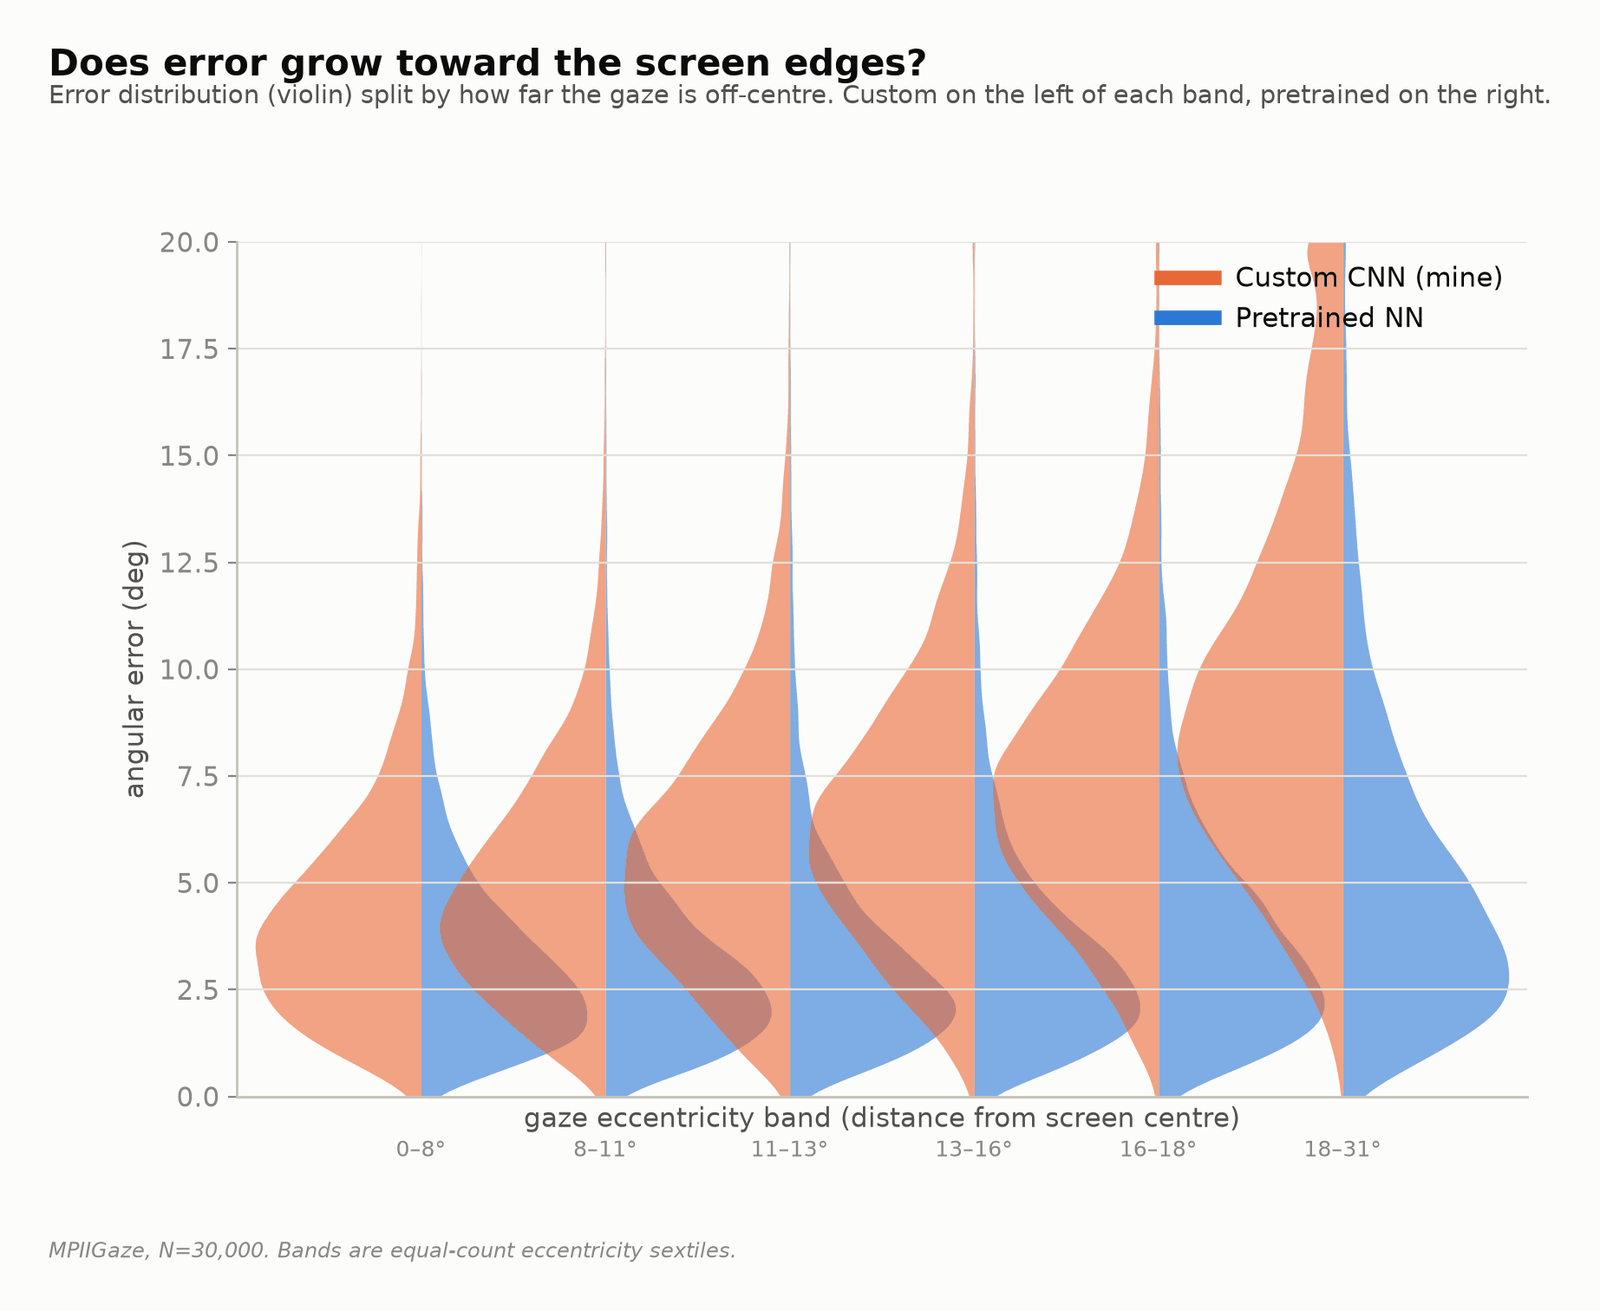
\includegraphics[width=\linewidth]{figures/gaze_G6_eccentricity_ridgeline.png}
\caption{Error versus eccentricity --- angular-error distributions stratified by how far off-centre the true gaze lies.}
\label{fig:9}
\end{figure}

Both models degrade off-axis, which has an optical basis --- foreshortening and eyelid occlusion reduce informative pixels per unit of angular change --- but the ridgelines separate by a broadly constant factor rather than diverging. That distinction discriminates between two accounts. A purely optical limit acts additively on both models,

\begin{equation}
\label{eq:210}
e_M(\|\theta \|) = e_M(0) + \kappa _{\mathrm{opt}}(\|\theta \|) \implies e_A - e_R \;\text{constant in}\; \|\theta \| ,
\end{equation}

whereas a gain deficit acts multiplicatively by \EQREF{194},

\begin{equation}
\label{eq:211}
e_M(\|\theta \|) \approx ( 1 - s_M ) \|\theta \| + \nu _M \implies e_A / e_R \;\text{approximately constant in}\; \|\theta \| .
\end{equation}

The data support \EQREF{211}, so the proposed network has no peripheral failure mode to repair --- only a uniformly contracted response, which is good news for the screen-edge behaviour the deployed 1.2 expansion factor is designed to reach.

\FIGREF{10} exposes the axis asymmetry that pooled error conceals.

\begin{figure}[pos=htbp]
\centering
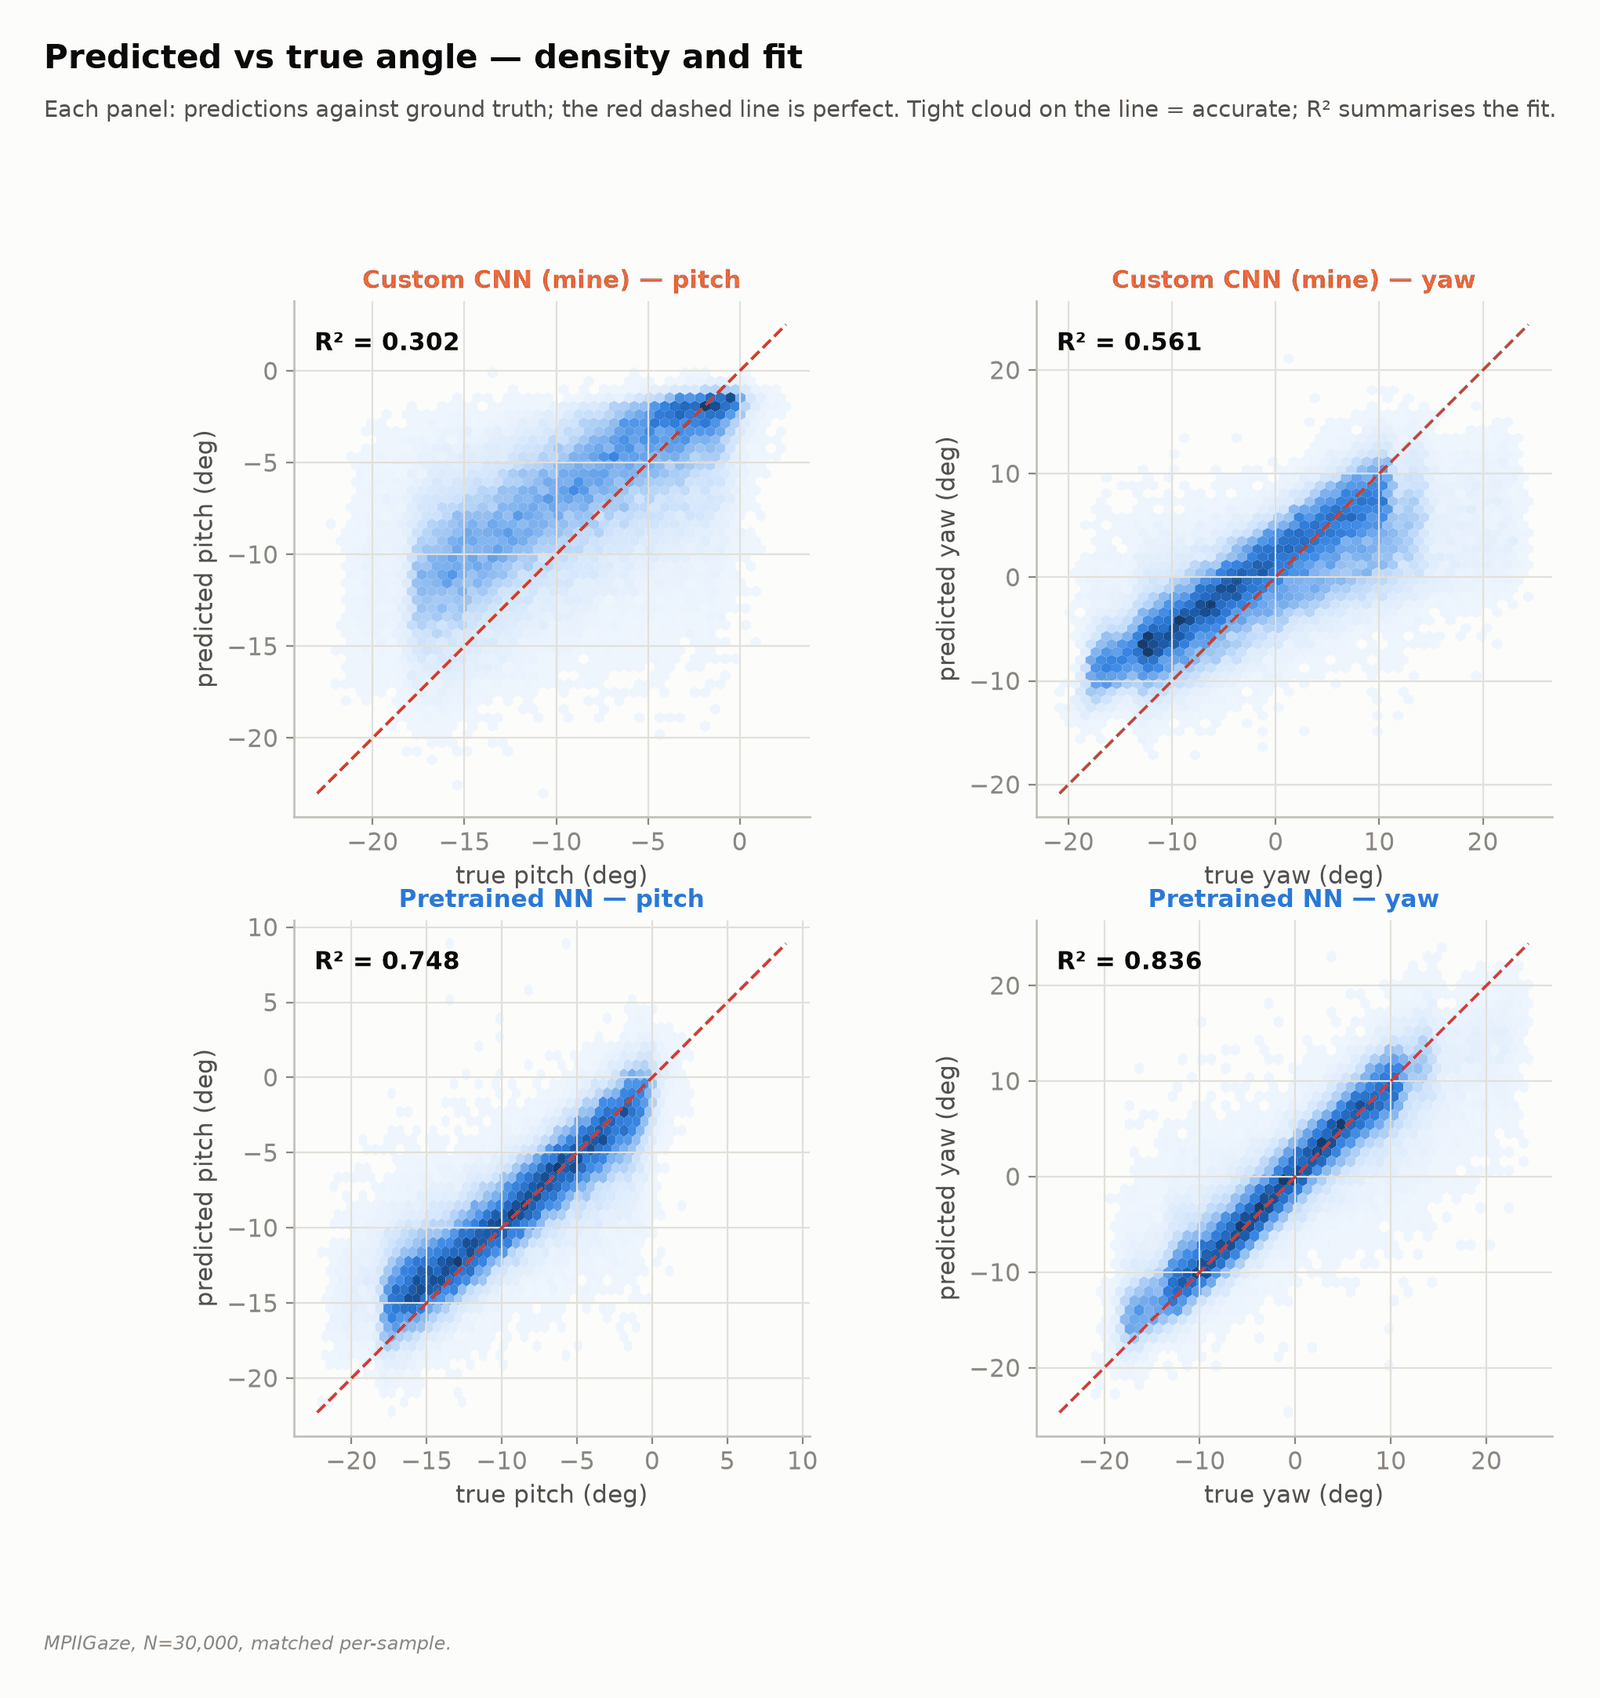
\includegraphics[width=\linewidth]{figures/gaze_G7_true_vs_pred.png}
\caption{Predicted versus true --- density-weighted regression fits with coefficient of determination for pitch and yaw.}
\label{fig:10}
\end{figure}

By \EQREF{153} the proposed network attains R$^{2}$ = 0.302 in pitch and 0.561 in yaw against 0.748 and 0.836. Because its fitted gain is essentially identical on both axes by \EQREF{191}, the R$^{2}$ disparity cannot be a gain effect. Writing \EQREF{153} in terms of the shrinkage model,

\begin{equation}
\label{eq:212}
R^{2}_a = \hat{s}_a^{2} \sigma _{\theta _a}^{2} / ( \hat{s}_a^{2} \sigma _{\theta _a}^{2} + \sigma _{\zeta _a}^{2} ) ,
\end{equation}

equal $\hat{s}_{a}$ on both axes forces the disparity into the residual variance $\sigma_{\zeta^{2}}$. The physical explanation is direct: vertical gaze is signalled through eyelid aperture and iris occlusion, cues confounded with blink state and individual eyelid morphology, whereas horizontal gaze produces a clean identity-invariant lateral translation of the iris. Pitch is thus the axis most contaminated by identity-specific appearance and the one expected to suffer most under a nine-identity training set --- a prediction the attribution analysis of \FIGREF{15} below confirms mechanistically. It also explains why the deployed vertical gain (3.4) is set higher than would be needed for a symmetric estimator.

\FIGRANGE{11}{14} re-render the same per-sample data as continuous fields. They add no measurement, but three of the claims above --- isotropy, the dominance of incoherent over coherent displacement, and residual anisotropy --- are claims about \emph{joint} structure and are tested most directly here.

\begin{figure}[pos=htbp]
\centering
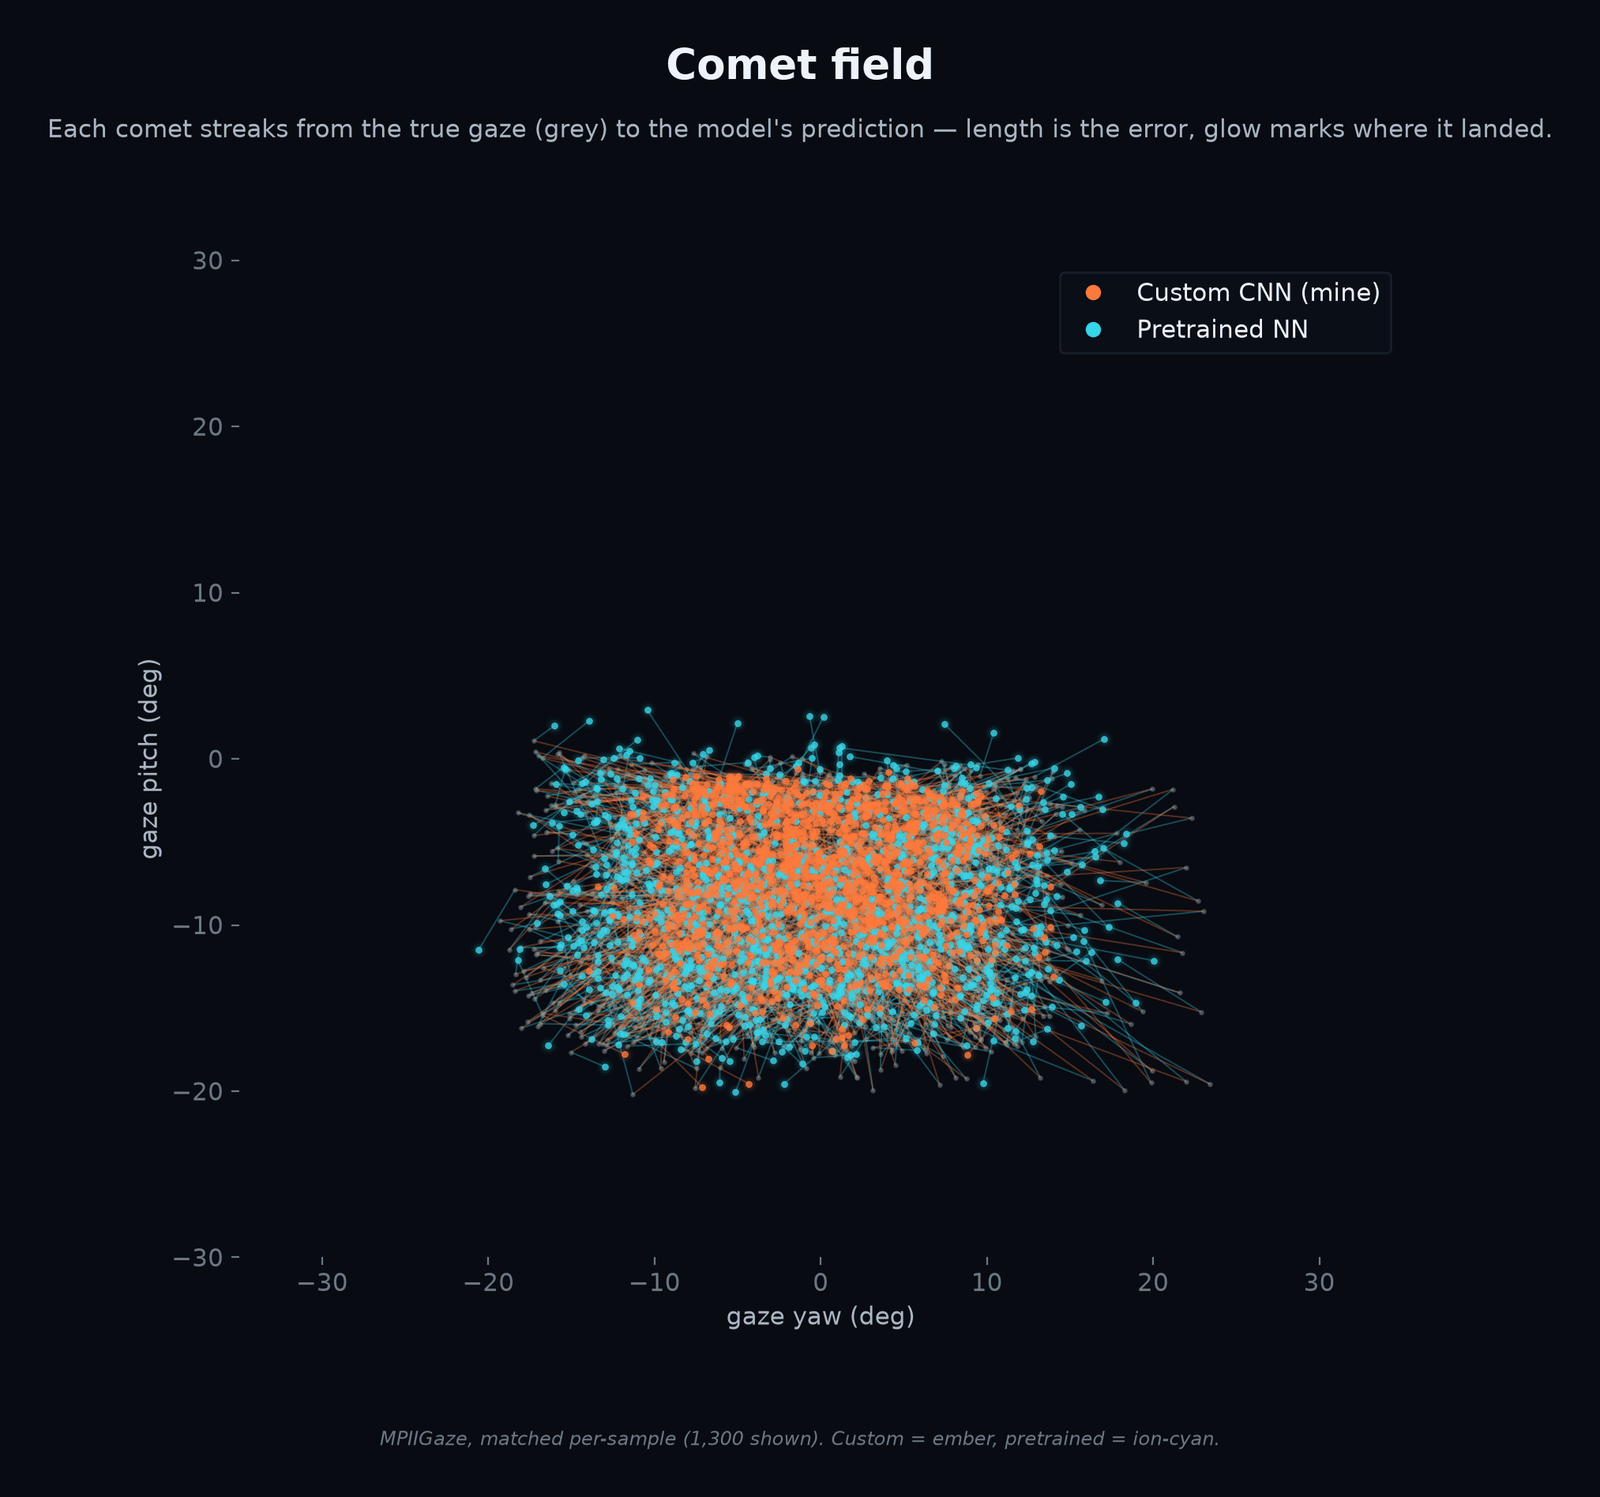
\includegraphics[width=\linewidth]{figures/figures_art_gaze_GA1_comet_field.png}
\caption{Comet field --- every held-out sample drawn as a streak from its true gaze direction to the model's prediction; streak length is the per-sample angular error.}
\label{fig:11}
\end{figure}

Retaining every displacement rather than their mean separates coherent from incoherent error. Decomposing the displacement field,

\begin{equation}
\label{eq:213}
\begin{aligned}
\mathbf{u}(\theta ) = \hat{\theta } - \theta = \mathbb{E}[ \hat{\theta } - \theta | \theta ] + ( \hat{\theta } - \mathbb{E}[ \hat{\theta } | \theta ] ) , \\ 
\text{coherent incoherent}
\end{aligned}
\end{equation}

the streaks share a common upward coherent component of 1.987$^{\circ}$ but their residual directions are largely uncorrelated. Coherent displacement is calibration error and is removable by the deployed polynomial; incoherent displacement is representational noise and is not, passing instead to the one-euro filter. The visual dominance of the incoherent component is the geometric reason exact bias removal recovers only 6.5 \% by \EQREF{196}, and it predicts that most of the deployed system's gaze quality is bought by temporal smoothing rather than by calibration.

\begin{figure}[pos=htbp]
\centering
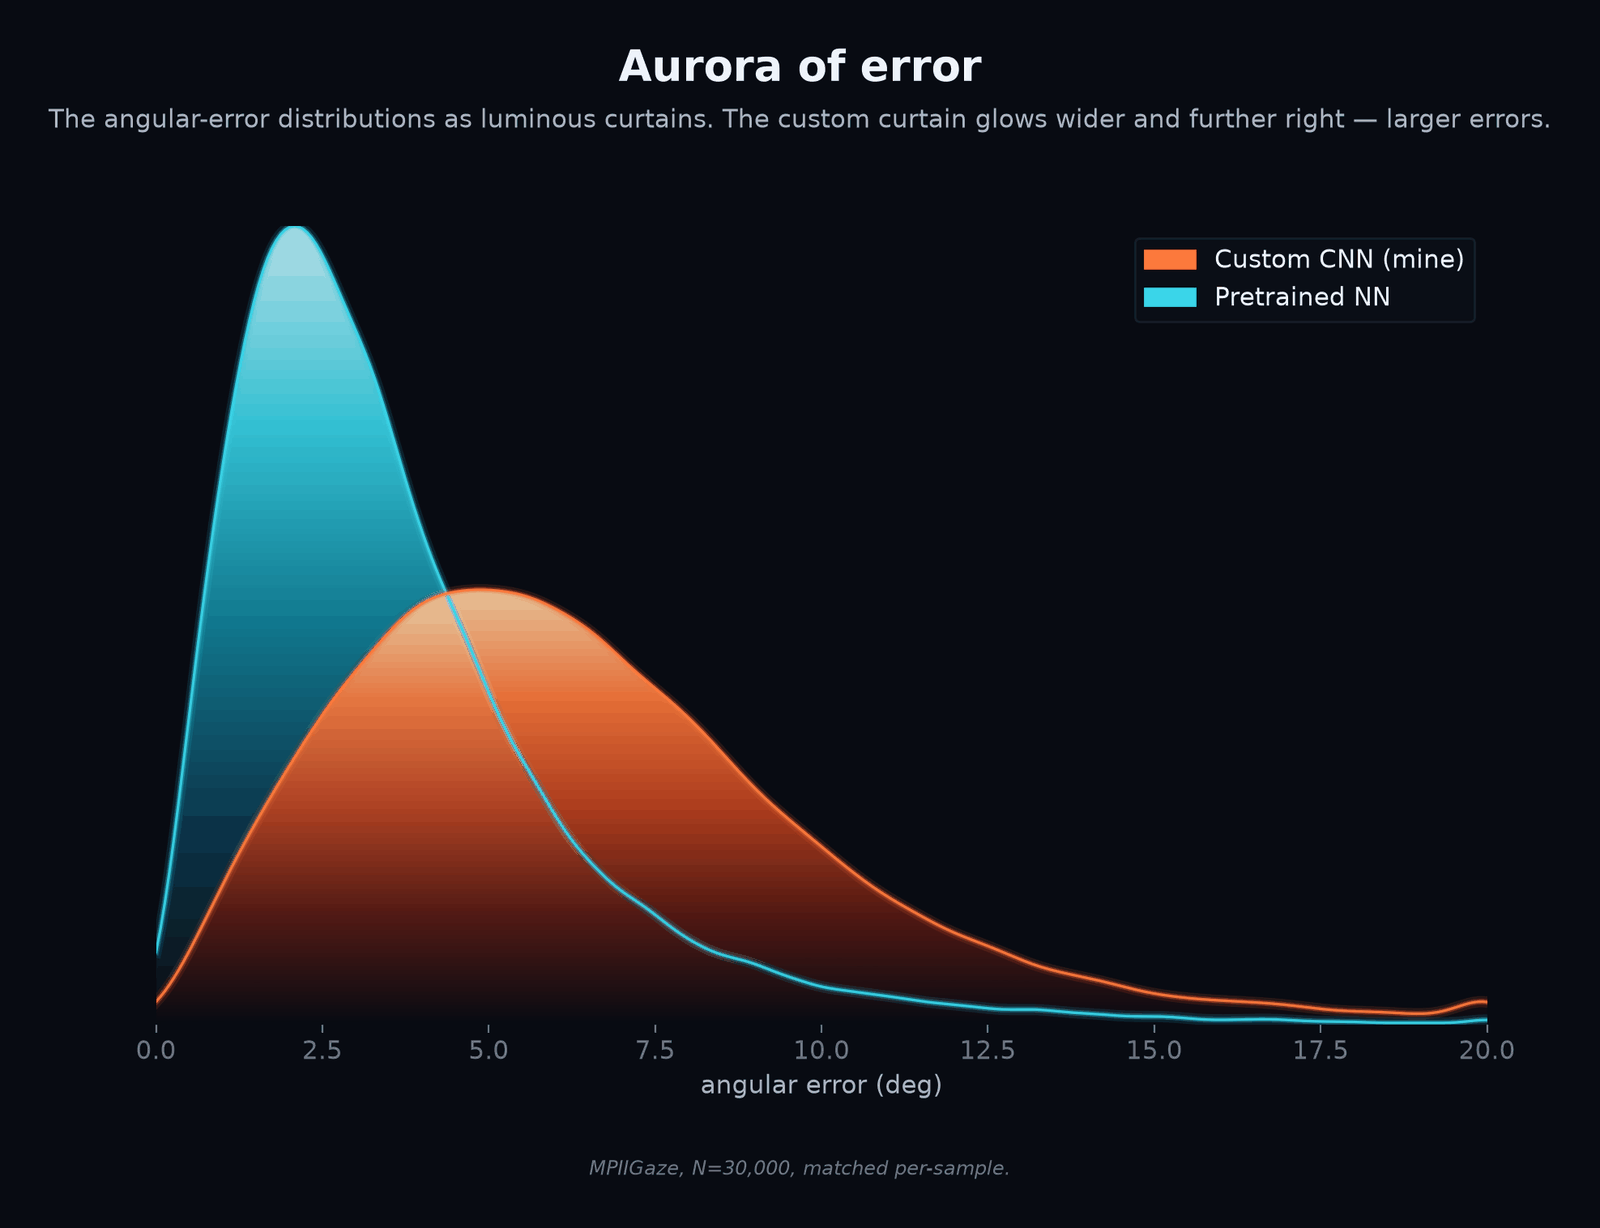
\includegraphics[width=\linewidth]{figures/figures_art_gaze_GA2_aurora.png}
\caption{Aurora of error --- the angular-error distributions of both models rendered as luminous density curtains.}
\label{fig:12}
\end{figure}

The curtains overlap substantially despite a 2.818$^{\circ}$ mean separation --- the graphical form of d = 0.854, large but far from disjoint, and consistent with the 18.86 \% win rate. Both distributions are right-skewed (means 6.439$^{\circ}$ and 3.621$^{\circ}$ against medians 5.873$^{\circ}$ and 2.985$^{\circ}$), with skew ratios

\begin{equation}
\label{eq:214}
\mathrm{mean}/\mathrm{median}: 6.439/5.873 = 1.096 (A) , 3.621/2.985 = 1.213 (R) ,
\end{equation}

so neither model's typical behaviour is captured by its mean, and median-based reporting is the safer convention for this task. The skew is proportionally greater for the baseline, indicating its advantage is realised most strongly on the bulk of easy samples --- precisely where a correctly-scaled estimator gains over a contracted one, since by \EQREF{194} the contracted estimator's systematic error vanishes only at $\theta$ = 0.

\begin{figure}[pos=htbp]
\centering
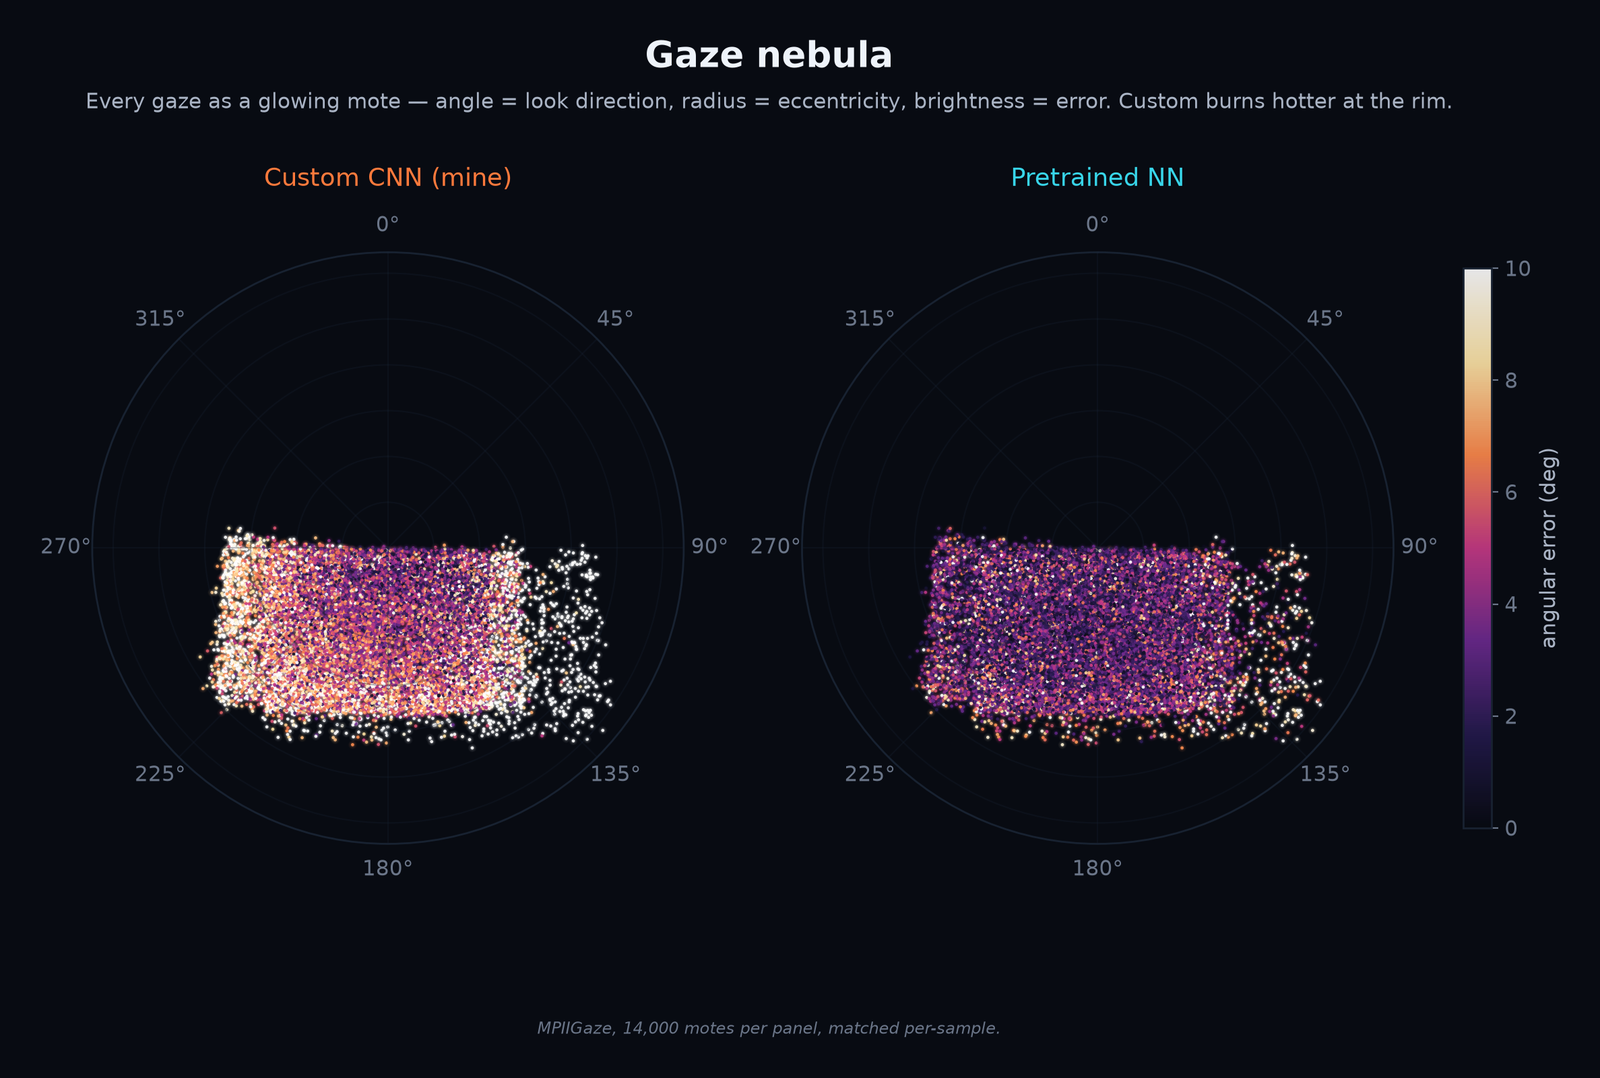
\includegraphics[width=\linewidth]{figures/figures_art_gaze_GA3_nebula.png}
\caption{Gaze nebula --- every held-out gaze as a point placed by direction and eccentricity, with brightness encoding its error.}
\label{fig:13}
\end{figure}

Collapsing the stratifications of Figs. 4 and 8 into one field makes the governing law testable rather than inferred: brightness rises with radius and is uniform in angle. Error is a function of eccentricity alone with no azimuthal dependence --- the exact signature of the (1 -- s)$\|\theta\|$ term of \EQREF{194} and the single strongest confirmation that the gaze deficit is a resolution limit rather than a geometric fault, since any crop or normalisation error would introduce azimuthal asymmetry.

\begin{figure}[pos=htbp]
\centering
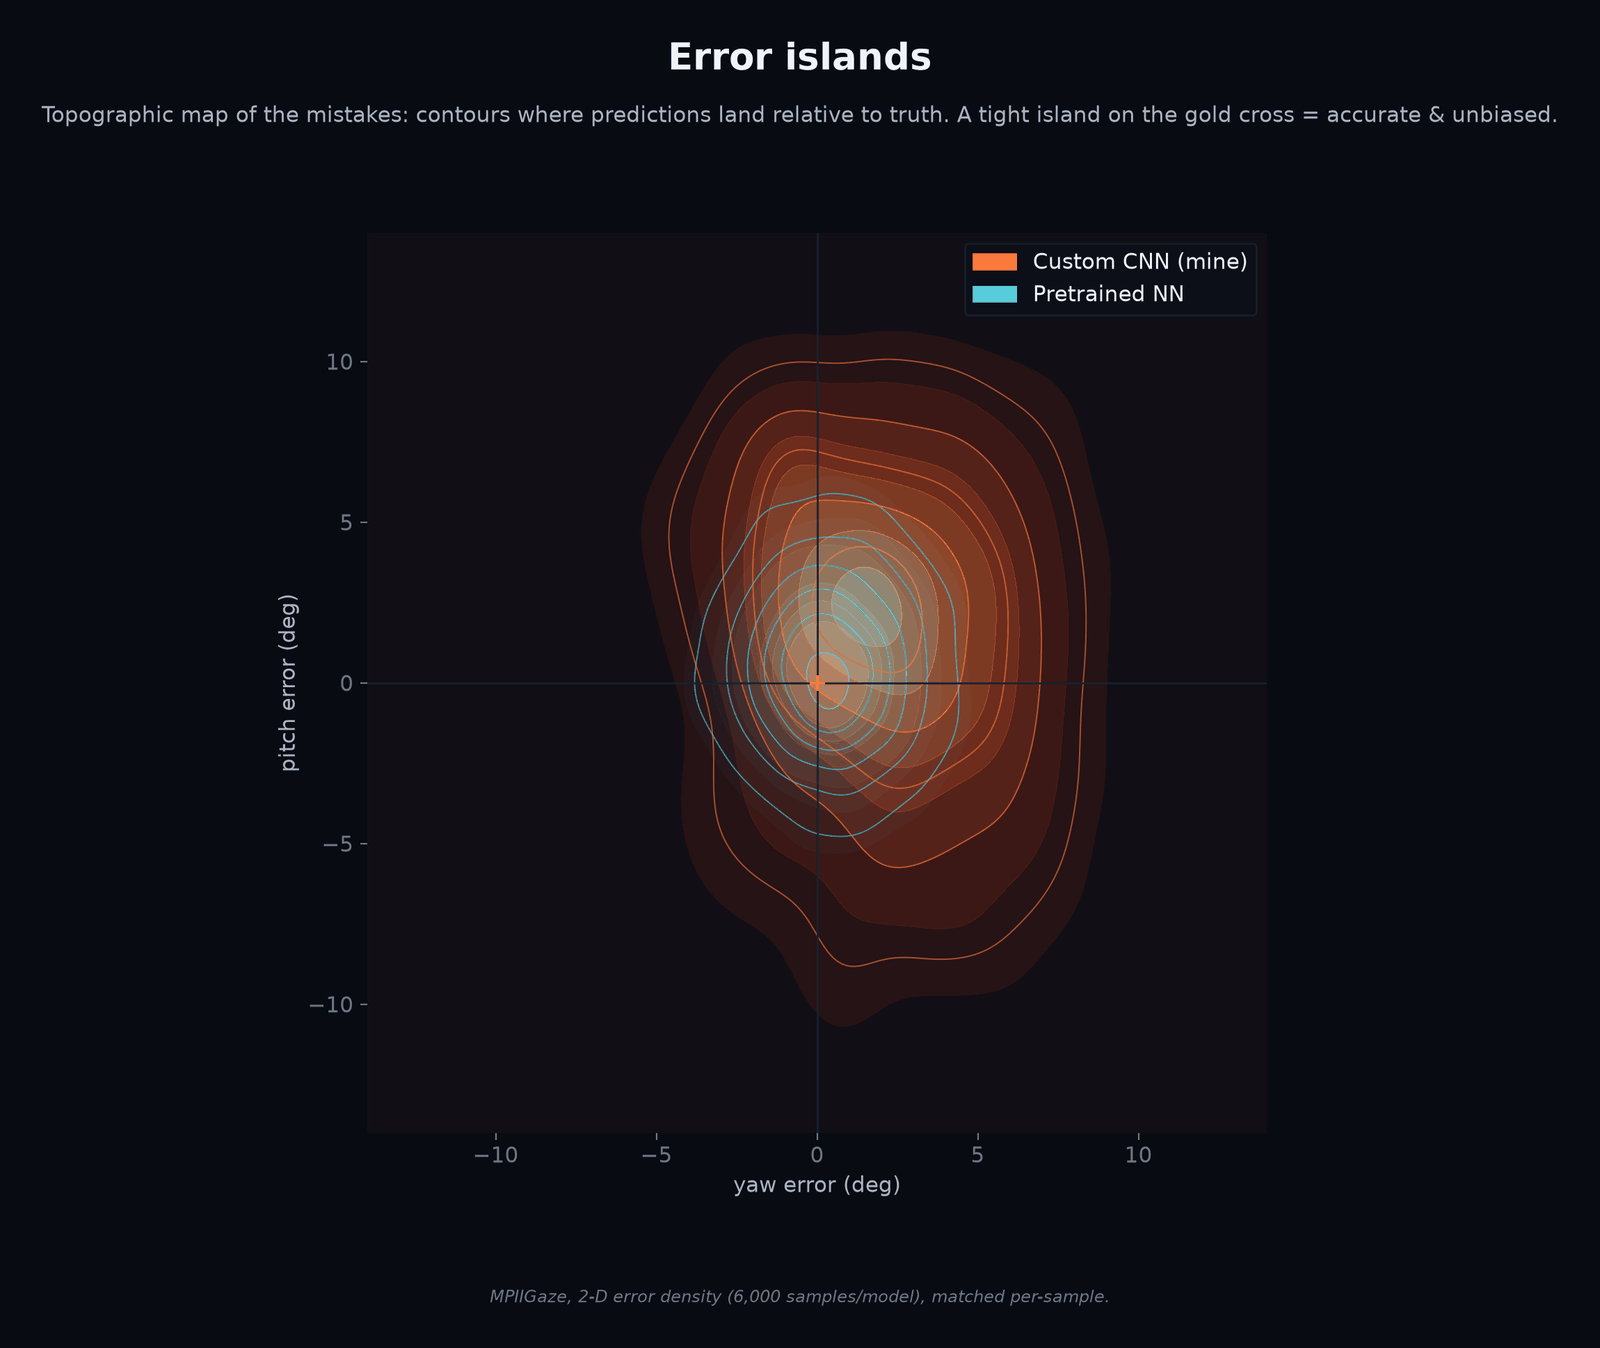
\includegraphics[width=\linewidth]{figures/figures_art_gaze_GA4_error_islands.png}
\caption{Error islands --- density contours of predictions relative to ground truth for each model; a tight island centred on the cross is accurate and unbiased.}
\label{fig:14}
\end{figure}

The proposed network's island is displaced by the 1.987$^{\circ}$ pitch offset and elongated in yaw at a standard-deviation ratio

\begin{equation}
\label{eq:215}
\begin{aligned}
\sigma _{\mathrm{yaw}}/\sigma _{\mathrm{pitch}} = 5.988/3.914 = 1.53 (A) , \\
3.675/2.596 = 1.42 (R) .
\end{aligned}
\end{equation}

The anisotropy is therefore partly intrinsic to the task and partly amplified by the proposed network --- consistent with the horizontally-tuned operator identified next, since an operator optimised for horizontal displacement necessarily places its widest residual along the horizontal axis, and consistent in turn with the deployed controller using different horizontal and vertical gains.

\subsubsection{What the network computes}

Accuracy establishes that a network is right; it does not establish that it is right for a transferable reason. Attribution follows Section 3.10: Integrated Gradients \CITE{ig} against a zero baseline over 32 steps, computed directly on the deployed TorchScript module, with the input partitioned into a 4 $\times$ 4 grid by \EQREF{139} so that each region assumes the role of a feature. Completeness \EQREF{138} makes the decompositions exact rather than indicative.

\begin{figure}[pos=htbp]
\centering
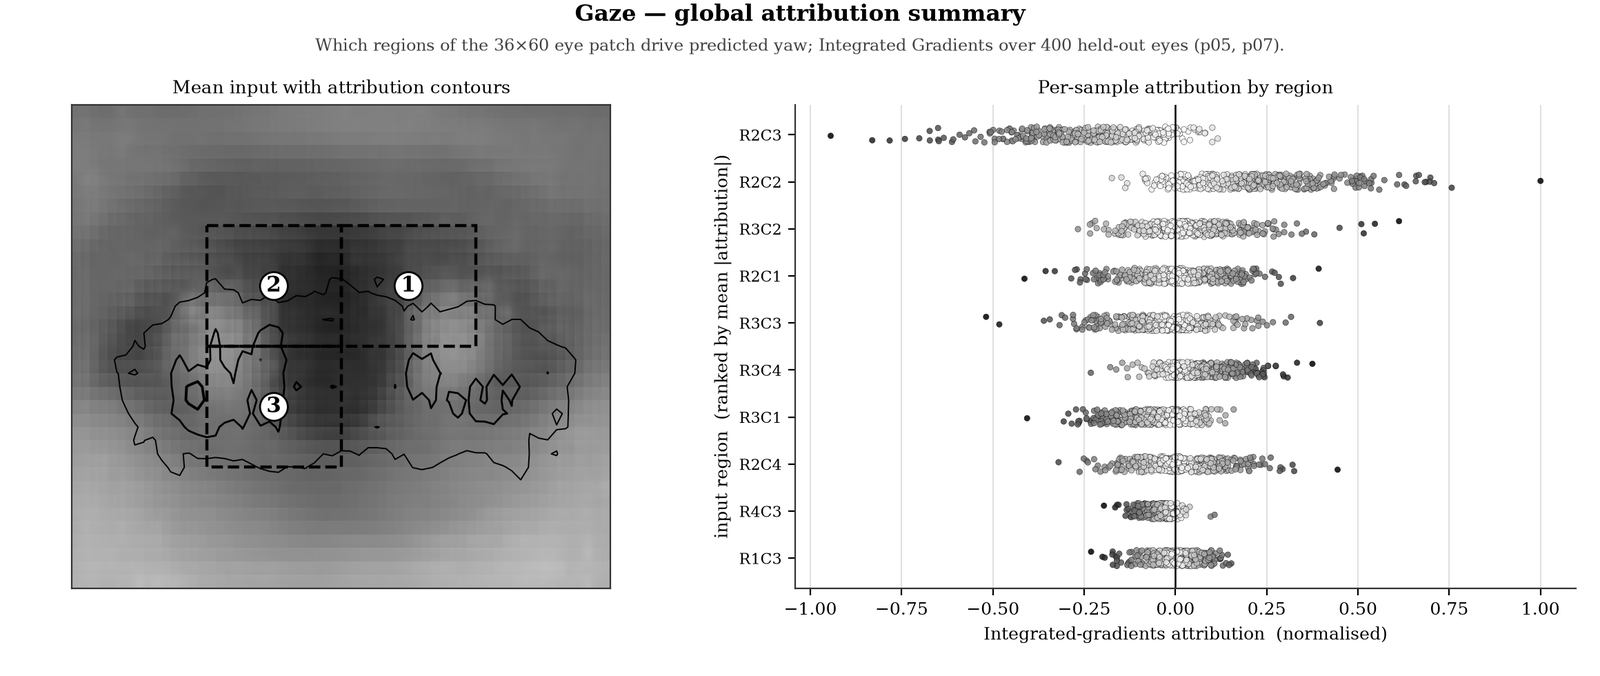
\includegraphics[width=\linewidth]{figures/attribution_gaze_A1_summary.png}
\caption{Gaze --- global attribution summary for predicted yaw over the 36 $\times$ 60 eye patch, regions ranked by mean absolute attribution.}
\label{fig:15}
\end{figure}

The two dominant regions, R2C3 and R2C2, sit side by side across the vertical midline carrying opposite-signed attribution. The network has therefore learned a \textbf{signed differential operator} across the midline,

\begin{equation}
\label{eq:216}
\begin{aligned}
F_{\mathrm{yaw}}(x) \approx \Sigma _{k \in \;\text{left}} w_k \langle x, \\
\phi _k\rangle - \Sigma _{k \in \;\text{right}} w_k \langle x, \phi _k\rangle , \\
w_k > 0 ,
\end{aligned}
\end{equation}

which is exactly the computation yaw estimation requires, since horizontal gaze is encoded by iris displacement relative to the eye-corner frame. Attribution concentrates in the horizontal band with little vertical structure, independently explaining the axis asymmetry of \FIGREF{10}: capacity was allocated horizontally, so pitch is served by whatever vertical signal survives incidentally. That the operator is \emph{differential} rather than absolute is what makes it robust to the illumination variation a home webcam delivers, since a differential operator annihilates the additive component of the photometric family that \EQREF{15} normalises.

\begin{figure}[pos=htbp]
\centering
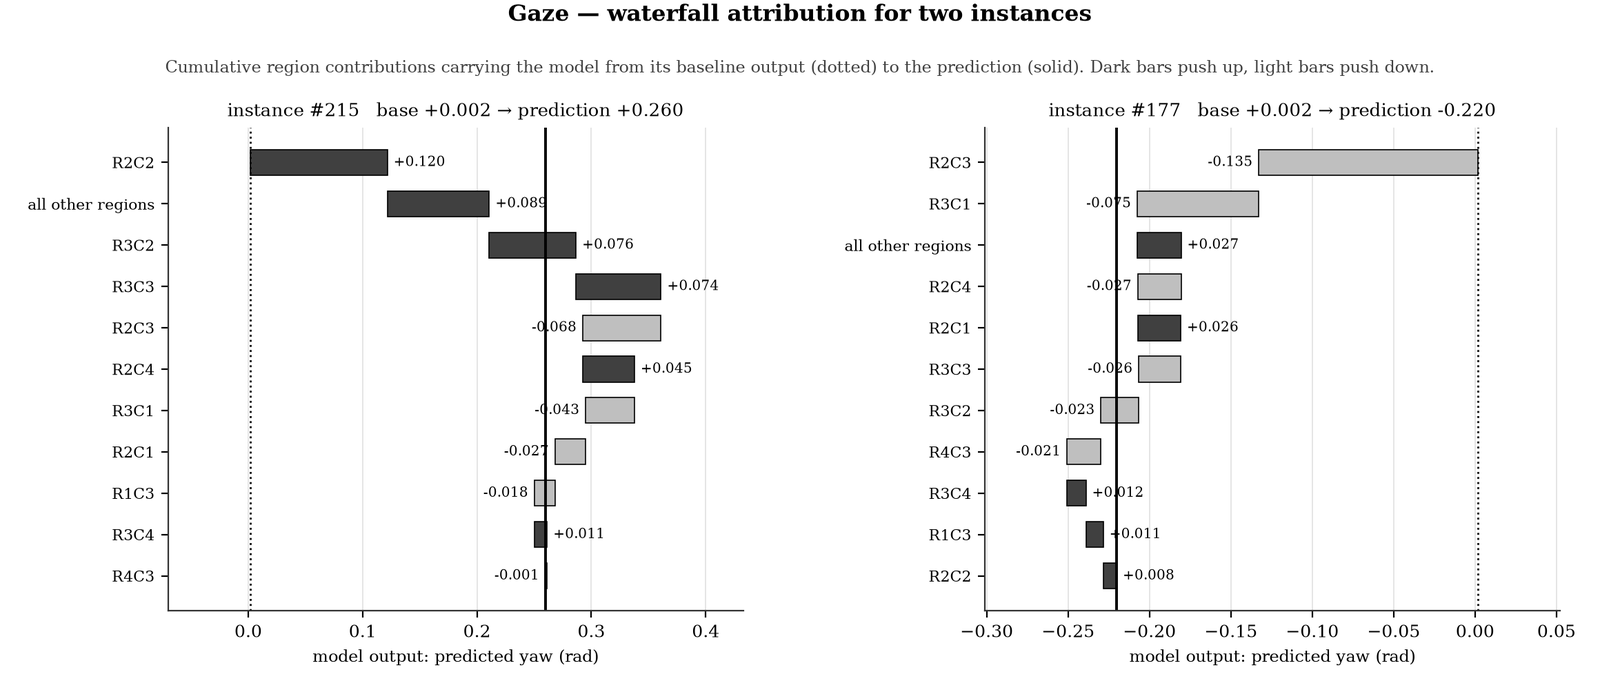
\includegraphics[width=\linewidth]{figures/attribution_gaze_A2_waterfall.png}
\caption{Gaze --- waterfall attribution for two extreme instances of predicted yaw.}
\label{fig:16}
\end{figure}

Extreme instances are carried to their predictions by opposing contributions from the same midline pair, confirming the differential structure operates per instance rather than emerging from averaging. The residual regions contribute a small consistently-signed offset --- the attribution-space counterpart of the +1.987$^{\circ}$ bias of \FIGREF{5} --- which localises that bias in a distributed background term rather than in the discriminative operator, and explains why removing it recovers only 6.5 \% of angular error.

\begin{figure}[pos=htbp]
\centering
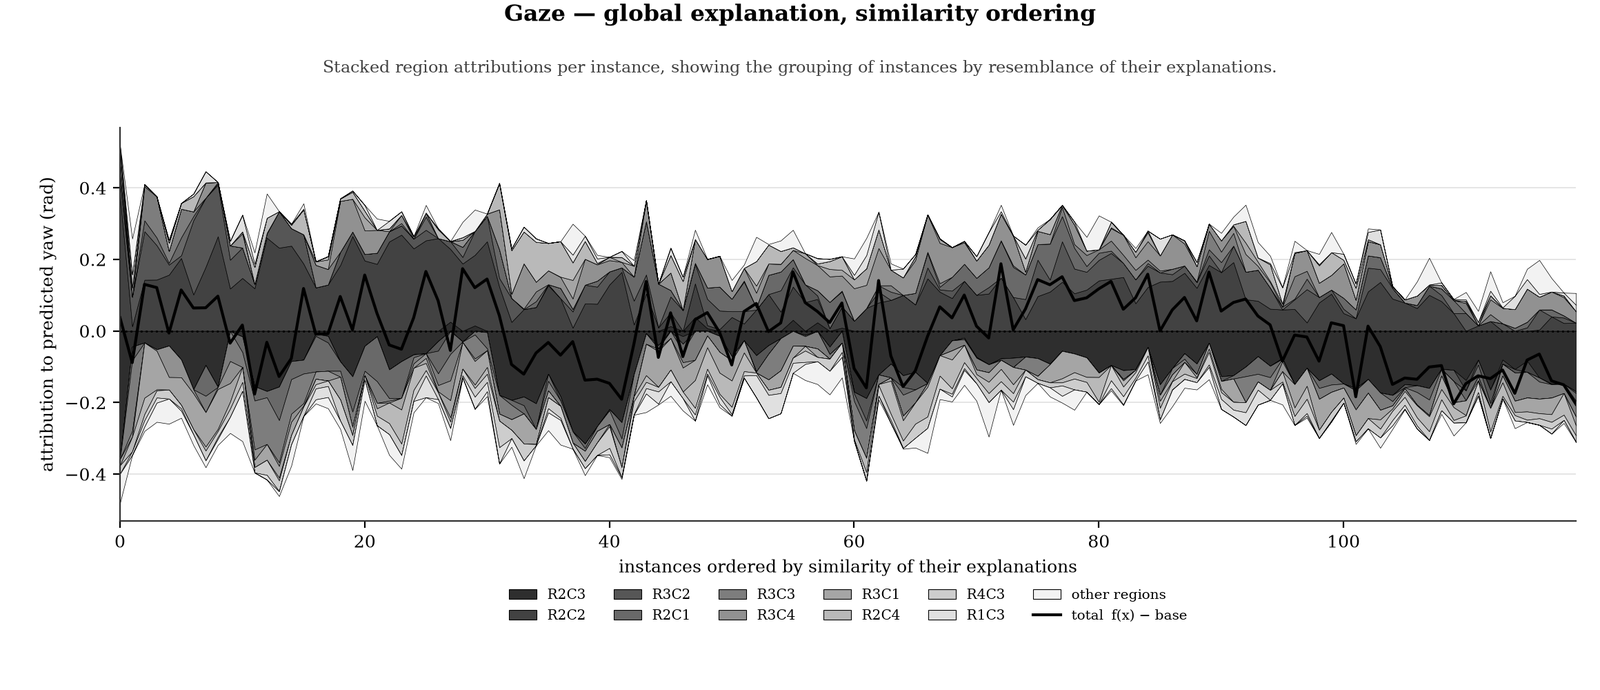
\includegraphics[width=\linewidth]{figures/attribution_gaze_A3_similarity.png}
\caption{Gaze --- global explanation under similarity ordering.}
\label{fig:17}
\end{figure}

Similarity ordering produces a smooth continuum rather than discrete blocks, which is correct for regression over a continuous target: neighbouring gaze angles should induce neighbouring explanations. Formally, the explanation map is approximately Lipschitz,

\begin{equation}
\label{eq:217}
\| \mathrm{Attr}(\cdot ; x_{1}) - \mathrm{Attr}(\cdot ; x_{2}) \| \leq L \| \theta (x_{1}) - \theta (x_{2}) \| ,
\end{equation}

with no discontinuity anywhere along the ordering. This rules out piecewise or identity-conditioned strategy switching, so the elevated error of Section 5.2.2 is uniform representational imprecision rather than a mixture of a good rule and a bad one --- the attribution-level statement of the isotropic error field of \FIGREF{4}, reached by an independent route.

\begin{figure}[pos=htbp]
\centering
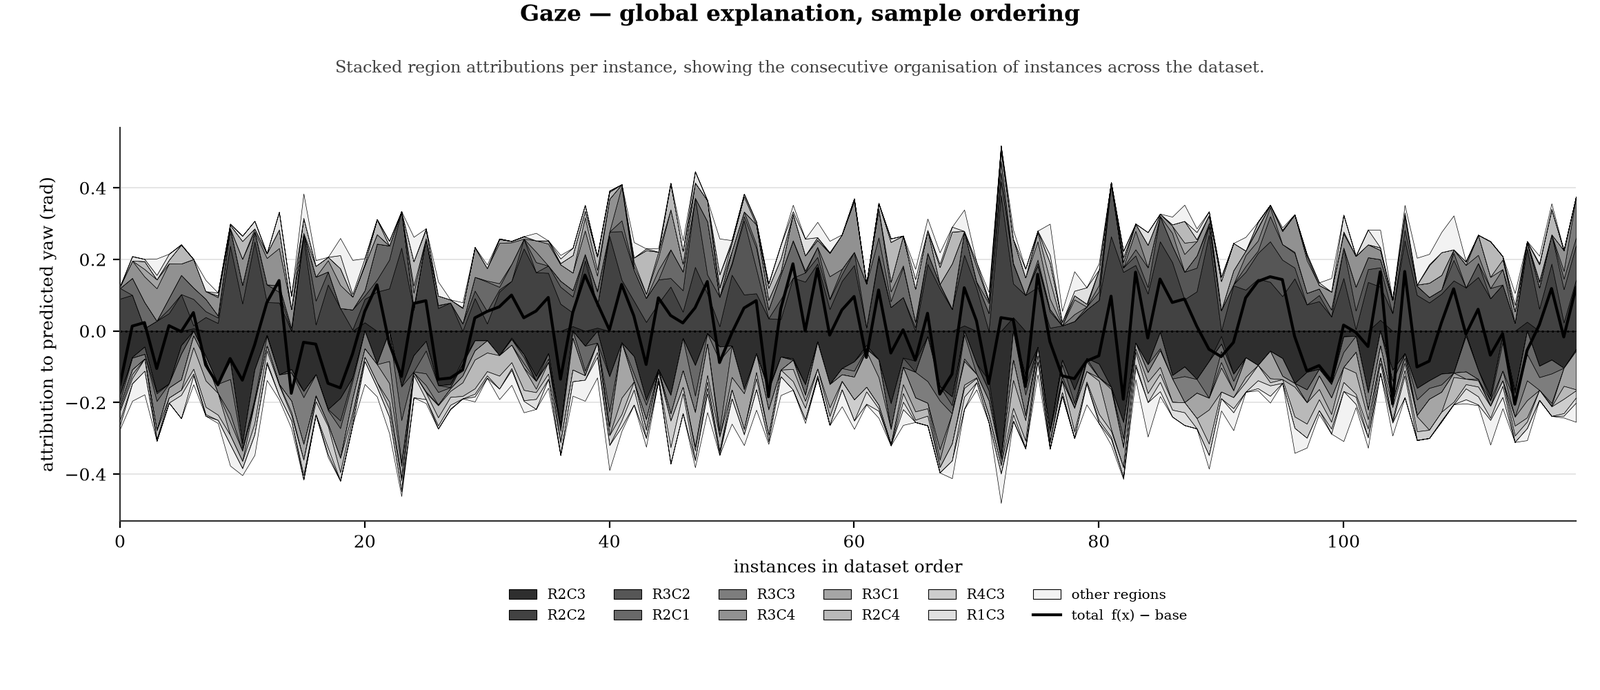
\includegraphics[width=\linewidth]{figures/attribution_gaze_A4_ordering.png}
\caption{Gaze --- global explanation under dataset ordering across held-out participants p05 and p07.}
\label{fig:18}
\end{figure}

Explanation structure stays coherent across the participant boundary while accuracy does not:

\begin{equation}
\label{eq:218}
e_{\mathrm{ang}}(p05) = 5.786^{\circ} , e_{\mathrm{ang}}(p07) = 7.138^{\circ} ,
\end{equation}

\begin{equation}
\label{eq:219}
\begin{aligned}
( \hat{s}_{\mathrm{pitch}}, \hat{s}_{\mathrm{yaw}} )(p05) = ( 0.586, 0.630 ) , \\
( \hat{s}_{\mathrm{pitch}}, \hat{s}_{\mathrm{yaw}} )(p07) = ( 0.377, 0.430 ) .
\end{aligned}
\end{equation}

The same operator is applied to both at substantially different gain, which localises identity sensitivity in the operator's \emph{calibration} rather than its \emph{form}. Writing the per-participant model as

\begin{equation}
\label{eq:220}
\begin{aligned}
\hat{\theta } = s(g) \cdot \mathcal{O}(x) + c(g) , \\
\mathcal{O} \;\text{fixed across g} , s(g) \;\text{varying} ,
\end{aligned}
\end{equation}

this is the mechanism behind the ceiling established next, and it is also the strongest available justification for the deployed per-user calibration stage: if identity enters as a scalar gain, a per-user scalar fit is the structurally correct remedy, and \EQREF{106}--\EQREF{107} is exactly such a fit.

\subsubsection{The ceiling is set by identity count, not sample count}

To test whether the residual error was data-limited, the network was retrained on 250,000 samples (175,199 training frames, 3.1$\times$ the configuration of Section 5.2.1). Validation error did not improve:

\begin{equation}
\label{eq:221}
6.32^{\circ} at 3.1\times \;\text{data}\; \mathrm{against} 5.81^{\circ} at 1\times ,
\end{equation}

a null result --- indeed a slight regression within run-to-run variation. The explanation follows directly from the effective-sample-size relation \EQREF{10}. Additional frames from the same nine identities are strongly correlated with those already present, so they raise n but not G, and by \EQREF{10}

\begin{equation}
\label{eq:222}
n_{\mathrm{eff}} = n / [ 1 + (\bar{n} - 1) \rho ] \to G / \rho as \bar{n} \to \infty ,
\end{equation}

which is bounded above by a constant depending only on the identity count. Extra frames therefore tighten the empirical risk estimate without enlarging the set of appearance modes the hypothesis must cover. \FIGREF{18} supplies the mechanism --- what nine identities fail to span is the \emph{range of gain} s(g) in \EQREF{220}, not the \emph{form} of the operator $\mathcal{O}$ --- and this explains why augmentation succeeded where more data failed: augmentation synthesises new imaging conditions by \EQREF{34}, while further frames of the same nine people supply none.

For the project this converts an open-ended tuning effort into a closed question. No further optimisation on MPIIGaze will close the gap to the pretrained baseline; only a corpus with more participants would, and Section 5.7 therefore recommends adopting the pretrained model rather than continuing to tune. It also predicts that gaze alone among the four modalities would benefit disproportionately from more participants rather than more frames --- a prediction the other three sections test implicitly, since none of them exhibits the same identity--gain coupling.

\FloatBarrier

\subsection{Head pose --- discrete gesture control}

Head pose does not position anything. It fires discrete application and tab gestures through the thresholded state machine of \ALGREF{6}: yaw triggers at 30$^{\circ}$ and releases at 12$^{\circ}$, pitch at 22$^{\circ}$ and 9$^{\circ}$, with a 650 ms dwell ($\approx$20 frames at the configured 30 fps by \EQREF{128}) and a 1,200 ms cooldown. Two consequences follow immediately from \EQREF{124}--\EQREF{129} and govern how the figures below should be read. Absolute mean absolute error is not the governing statistic --- what matters is whether error can carry a pose across a trigger boundary. And because the dwell requirement averages roughly twenty frames, \textbf{bias survives averaging while variance does not}, by \EQREF{129}, which inverts the usual ranking of the two.

Against the 6-D rotation-representation baseline on all 1,969 AFLW2000 faces, both models scoring the identical crop with no preprocessing asymmetry, the proposed network attains 7.367$^{\circ}$ MAE (median 4.185$^{\circ}$) against 3.482$^{\circ}$ (median 1.919$^{\circ}$). The paired statistics are

\begin{equation}
\label{eq:223}
\begin{aligned}
\bar{d} = 3.884^{\circ} \pm 0.272^{\circ} (95 \%) , \;\text{Cohen}\;'s d = 0.632 , \\
\;\text{Wilcoxon p}\; = 1.2 \times 10^{-226} ,
\end{aligned}
\end{equation}

\begin{equation}
\label{eq:224}
\begin{aligned}
\mathbb{P}[ e_A < e_R ] = 14.58 \% , r_{\mathrm{AR}} = 0.671 , \\
\bar{E}_{\mathrm{oracle}} = 3.222^{\circ} , \;\text{Gain}\;_{\mathrm{max}} = 7.5 \% .
\end{aligned}
\end{equation}

The error correlation of 0.671 is \emph{higher} than gaze's 0.491, and the oracle bound correspondingly tighter. Fusion is again unjustified, for the same structural reason: the two models fail on the same faces.

\textbf{The gain measurement transfers, with an instructive asymmetry.} Applying \EQREF{154} axis-wise,

\begin{equation}
\label{eq:225}
\begin{aligned}
\hat{s}_{\mathrm{yaw}}^A = 0.822 , \hat{s}_{\mathrm{pitch}}^A = 0.455 , \\
\hat{s}_{\mathrm{roll}}^A = 0.490 ,
\end{aligned}
\end{equation}

\begin{equation}
\label{eq:226}
\begin{aligned}
\hat{s}_{\mathrm{yaw}}^R = 1.046 , \hat{s}_{\mathrm{pitch}}^R = 0.768 , \\
\hat{s}_{\mathrm{roll}}^R = 0.877 .
\end{aligned}
\end{equation}

Yaw --- by far the widest-support axis in AFLW2000 --- is the only one reproduced at near-correct scale, and the pattern is exactly what the shrinkage account \EQREF{155} predicts. Since s* = $\sigma_{\theta^{2}}$/($\sigma_{\theta^{2}}$ + $\sigma_{\varepsilon^{2}}$), an axis with wide target support has large $\sigma_{\theta^{2}}$ and therefore a gain close to unity at fixed representational noise:

\begin{equation}
\label{eq:227}
\partial s* / \partial \sigma _{\theta} ^{2} = \sigma _{\varepsilon} ^{2} / ( \sigma _{\theta} ^{2} + \sigma _{\varepsilon} ^{2} )^{2} > 0 ,
\end{equation}

so wide target support supplies the gradient signal needed to resist contraction while the two narrow-support axes collapse to approximately half gain --- the same regime as gaze. Inverting \EQREF{158} per axis gives implied noise ratios

\begin{equation}
\label{eq:228}
\begin{aligned}
\hat{\sigma }_{\varepsilon} ^{2}/\sigma _{\theta} ^{2}: 0.217 (\text{yaw}) , \\
1.198 (\text{pitch}) , 1.041 (\text{roll}) ,
\end{aligned}
\end{equation}

confirming that the representation is markedly more informative about yaw than about the other two. That yaw is the best-scaled axis is fortunate for the interface, since yaw carries the two most-used gestures.

\FIGREF{19} begins with the per-axis error structure, which \TABREF{6} identifies as the decisive one.

\begin{figure}[pos=htbp]
\centering
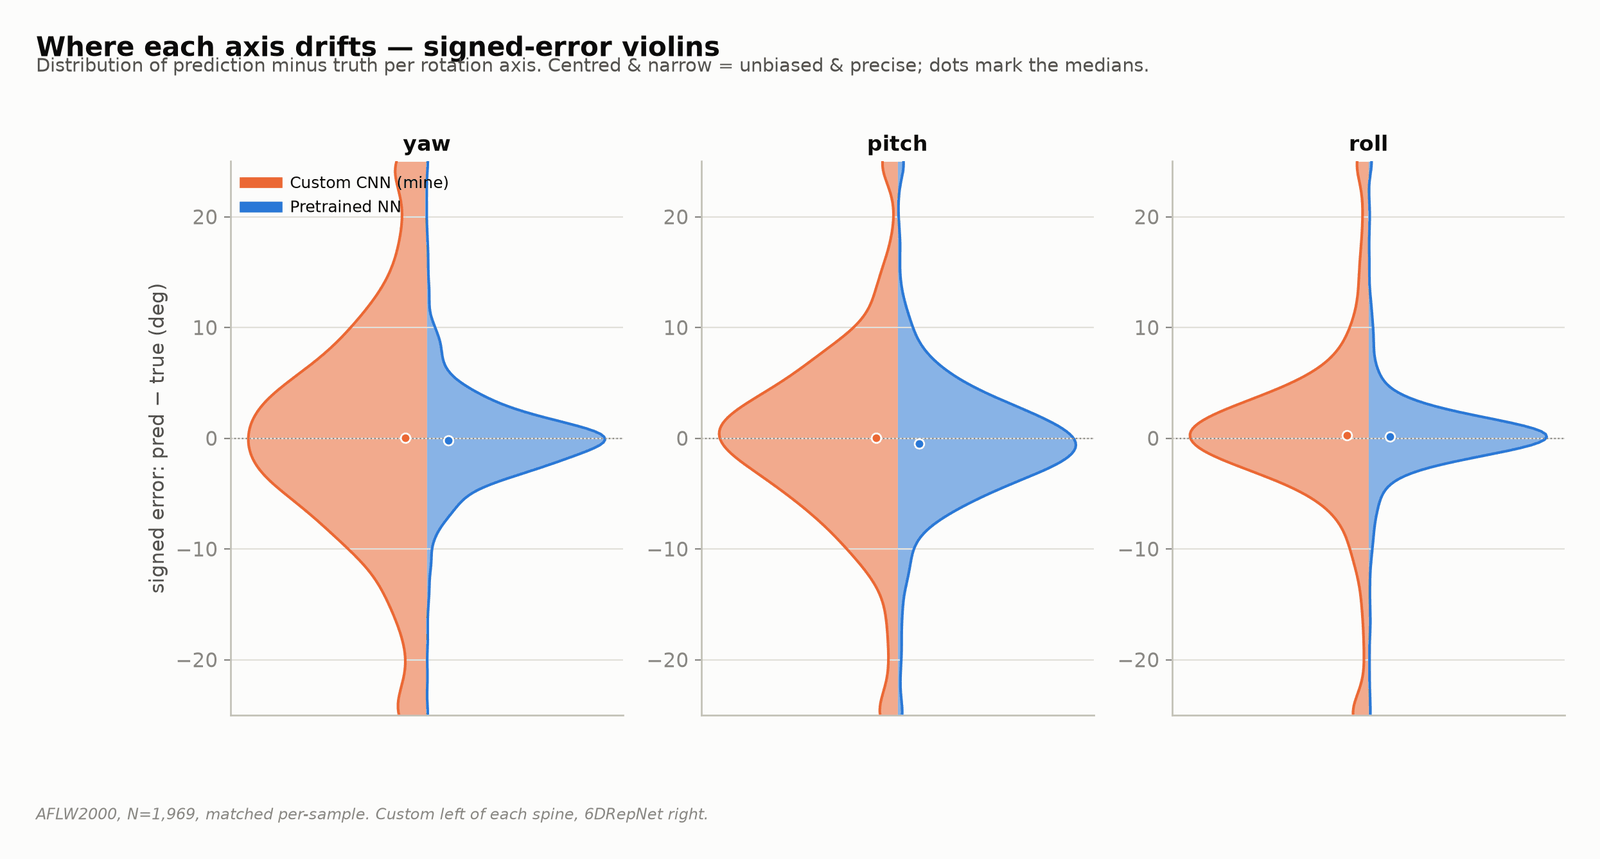
\includegraphics[width=\linewidth]{figures/headpose_H1_signed_violins.png}
\caption{Signed-error violins --- per-axis bias and spread, proposed network left of each spine and 6-D rotation baseline right.}
\label{fig:19}
\end{figure}

All three axes are essentially unbiased. By \EQREF{152},

\begin{equation}
\label{eq:229}
\begin{aligned}
\text{bias}\;^A = ( +0.109^{\circ} , -0.327^{\circ} , +0.062^{\circ} ) , \\
\;\text{bias}\;^R = ( -0.240^{\circ} , -0.624^{\circ} , +0.250^{\circ} ) ,
\end{aligned}
\end{equation}

so the entire deficit is spread, not offset --- the opposite decomposition to gaze, where a 1.987$^{\circ}$ pitch bias was the largest correctable term. This is the single most favourable result for the deployed gesture rule. Substituting the measured yaw spread into \EQREF{129} at the independence limit $\varrho$ = 0,

\begin{equation}
\label{eq:230}
\sigma _{\mathrm{dwell}}^{\mathrm{yaw}} = 12.49^{\circ} / \sqrt{20} = 2.79^{\circ} ,
\end{equation}

comfortably inside the 18$^{\circ}$ hysteresis band between the 30$^{\circ}$ trigger and the 12$^{\circ}$ release. Consecutive frames are correlated, so the true reduction is smaller: at a plausible $\varrho$ = 0.5 the same computation gives

\begin{equation}
\label{eq:231}
\sigma _{\mathrm{dwell}}^{\mathrm{yaw}} = ( 12.49/\sqrt{20} ) \cdot \sqrt{1.5/0.5} = 2.79 \times 1.732 = 4.84^{\circ} ,
\end{equation}

still well inside the band. Equation \EQREF{230} is therefore an upper bound on the benefit and \EQREF{231} a more realistic figure; the direction is unambiguous in either case, and it holds \textbf{only because the bias is near zero}. Had the network carried a gaze-like 2$^{\circ}$ offset, no amount of dwell averaging would have removed it, since \EQREF{129} attenuates only the variance term.

\FIGREF{20} aggregates four error measures across three axes.

\begin{figure}[pos=htbp]
\centering
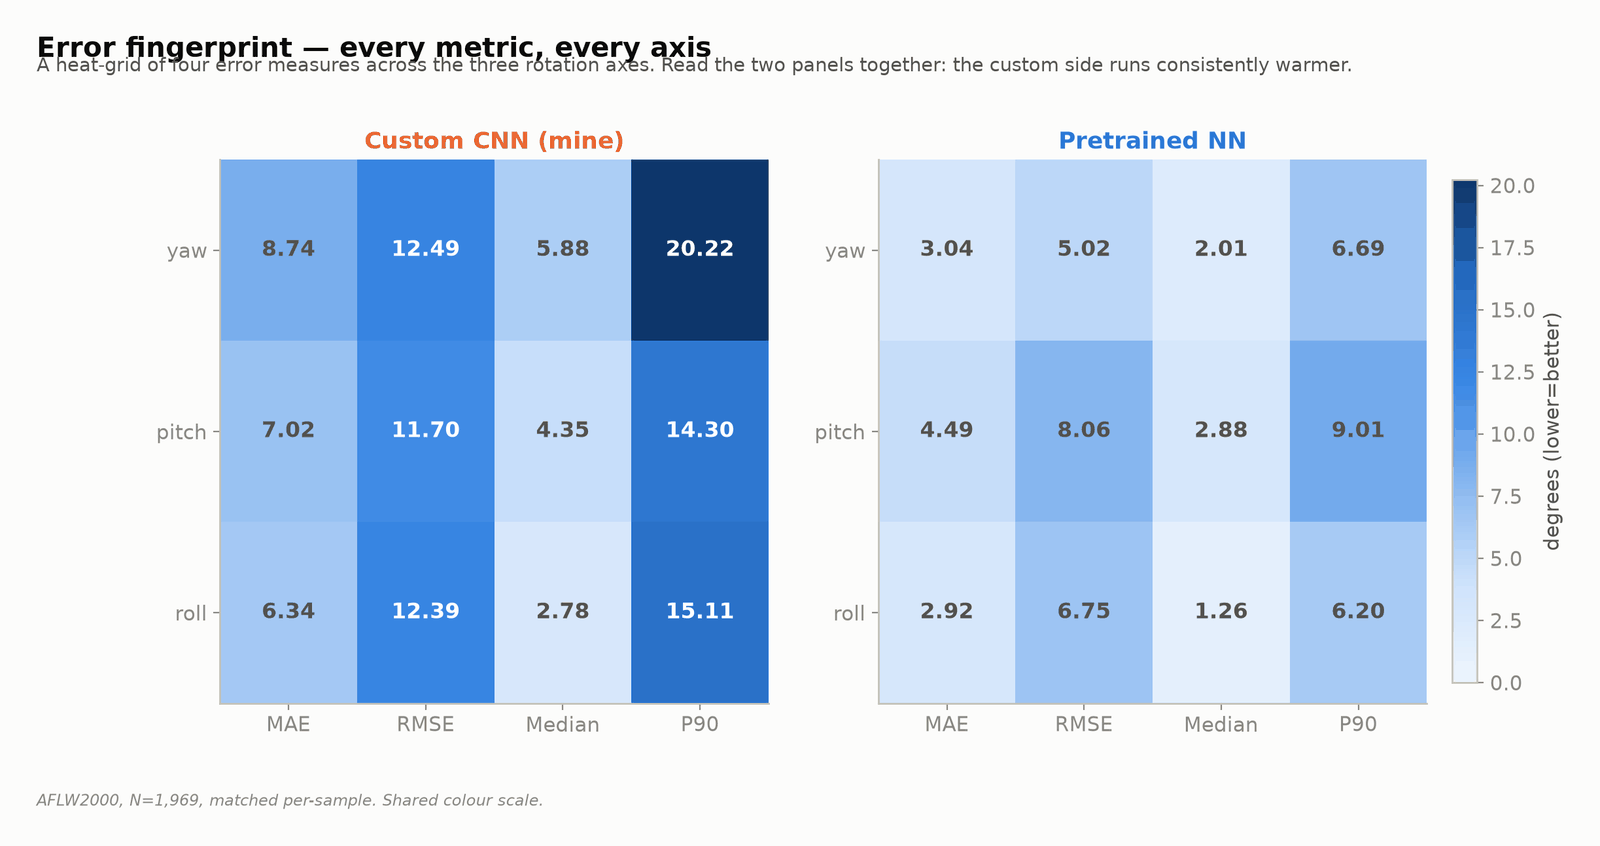
\includegraphics[width=\linewidth]{figures/headpose_H2_fingerprint.png}
\caption{Error fingerprint --- heat grid of four error measures across yaw, pitch and roll for each model.}
\label{fig:20}
\end{figure}

The fingerprint contains an axis-ranking inversion that the gain analysis resolves. The proposed network's MAE ordering is

\begin{equation}
\label{eq:232}
\text{yaw}\; (8.742^{\circ}) > \;\text{pitch}\; (7.023^{\circ}) > \;\text{roll}\; (6.335^{\circ}) ,
\end{equation}

while the baseline's is

\begin{equation}
\label{eq:233}
\text{pitch}\; (4.492^{\circ}) > \;\text{yaw}\; (3.039^{\circ}) > \;\text{roll}\; (2.916^{\circ}) .
\end{equation}

Yaw is simultaneously the proposed network's best-explained axis (R$^{2}$ = 0.875) and its worst in absolute degrees. The apparent contradiction dissolves once target ranges are considered, because the systematic error contributed by a gain deficit is (1 -- s)$\cdot\mathbb{E}$|$\theta$| by \EQREF{194}, and the two factors move oppositely across axes:

\begin{equation}
\label{eq:234}
\begin{aligned}
( 1 - \hat{s}_{\mathrm{yaw}} ) \cdot \mathbb{E}|\theta _{\mathrm{yaw}}| = 0.178 \times \mathbb{E}|\theta _{\mathrm{yaw}}| \\ 
\mathrm{against} \\ 
( 1 - \hat{s}_{\mathrm{pitch}} ) \cdot \mathbb{E}|\theta _{\mathrm{pitch}}| = 0.545 \times \mathbb{E}|\theta _{\mathrm{pitch}}| ,
\end{aligned}
\end{equation}

and since $\mathbb{E}$|$\theta_{\mathrm{yaw}}$| exceeds $\mathbb{E}$|$\theta_{\mathrm{pitch}}$| by more than a factor of three in AFLW2000, an 18 \% gain deficit over a $\pm$90$^{\circ}$ range costs more degrees than a 55 \% deficit over a range a fraction as wide. The inversion is therefore a \emph{units artefact} of comparing variance-normalised against absolute measures on axes with unequal support, and quoting either alone would mislead. For gesture triggering the absolute figure is the relevant one, which is why \TABREF{6} names it.

\FIGREF{21} maps error onto the pose manifold.

\begin{figure}[pos=htbp]
\centering
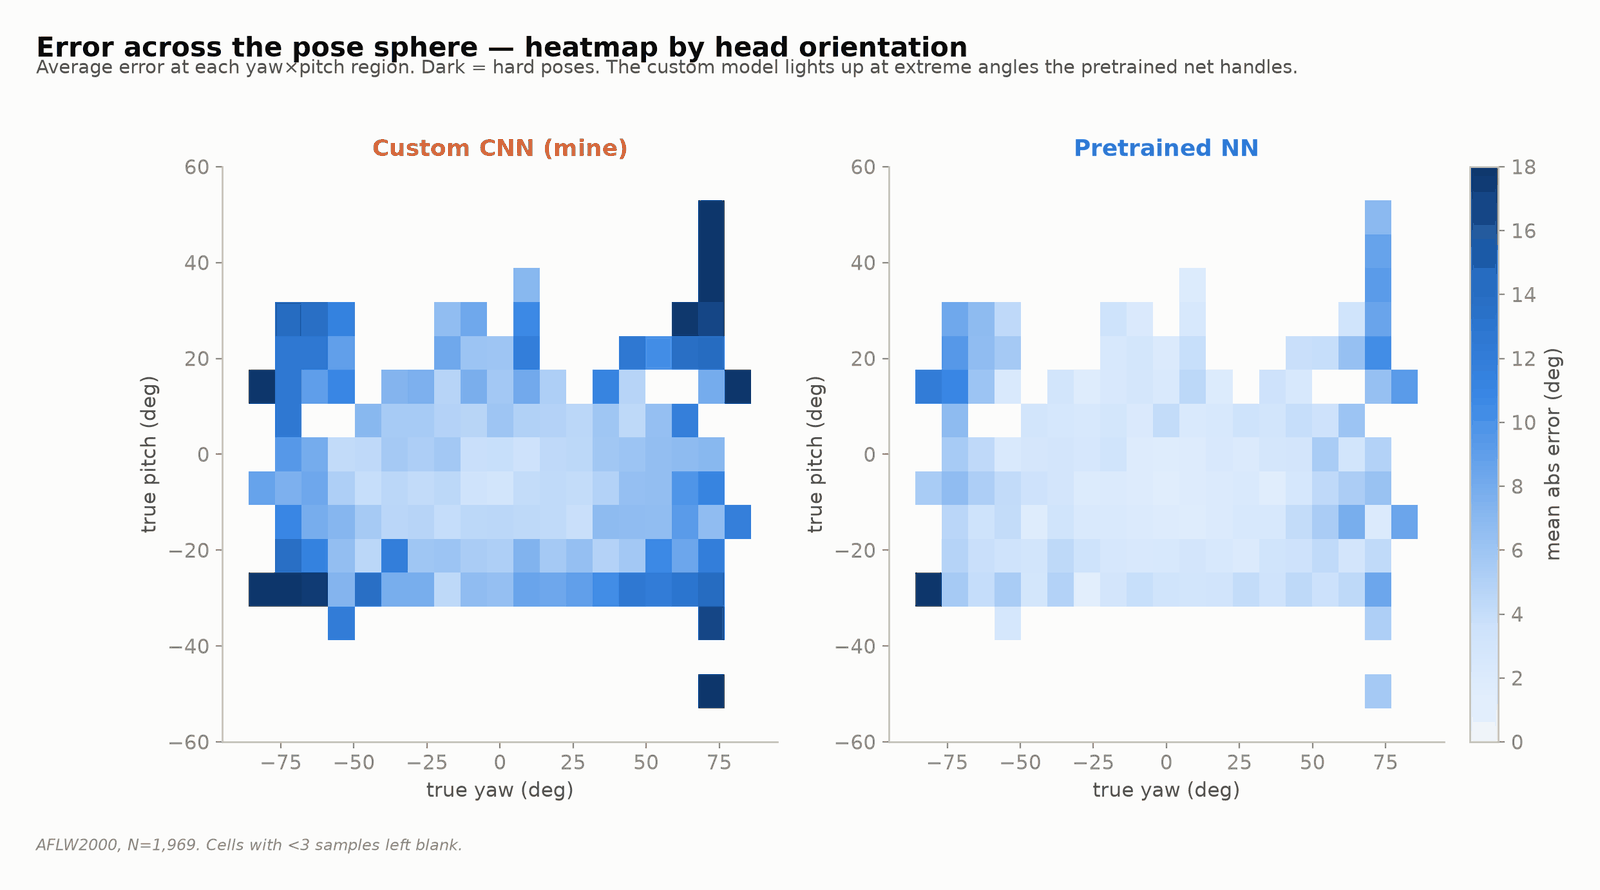
\includegraphics[width=\linewidth]{figures/headpose_H3_pose_heatmap.png}
\caption{Pose-sphere heat map --- mean error located in the yaw $\times$ pitch plane for each model.}
\label{fig:21}
\end{figure}

Three-axis mean error across four yaw bands is

\begin{equation}
\label{eq:235}
\begin{aligned}
A: 4.77^{\circ} (|\;\text{yaw}\;| < 15^{\circ}, n = 891)  \to \\
5.09^{\circ} (15\text{--}30^{\circ}, n = 420)  \to \\
8.08^{\circ} (30\text{--}60^{\circ}, n = 380)  \to \\
18.16^{\circ} (> 60^{\circ}, n = 278) ,
\end{aligned}
\end{equation}

\begin{equation}
\label{eq:236}
R: 2.35^{\circ} \to 2.47^{\circ} \to 3.81^{\circ} \to 8.20^{\circ} ,
\end{equation}

a 3.8$\times$ degradation for the proposed network against 3.5$\times$ for the baseline. The proposed-to-baseline ratio moves only from

\begin{equation}
\label{eq:237}
4.77/2.35 = 2.03 to 18.16/8.20 = 2.21
\end{equation}

across the entire manifold. Near-parallel degradation at a near-constant ratio is strong evidence against a localised failure mode: it is the manifold-level expression of \EQREF{211}, an approximately constant multiplicative loss of angular resolution everywhere. Critically for the interface, the region where error is largest --- beyond 60$^{\circ}$ --- lies well past the 30$^{\circ}$ trigger, so gesture reliability is governed by the two innermost bands, where error is 4.77$^{\circ}$ and 5.09$^{\circ}$ against an 18$^{\circ}$ hysteresis band. Expressing this as a margin,

\begin{equation}
\label{eq:238}
\mathrm{margin} = ( \theta _{\mathrm{on}} - \theta _{\mathrm{off}} ) / ( 2 \cdot e_{\mathrm{band}} ) = 18^{\circ} / ( 2 \times 5.09^{\circ} ) = 1.77 ,
\end{equation}

so a typical error must be nearly doubled before it can carry a pose across the band.

\FIGREF{22} gives the per-face view.

\begin{figure}[pos=htbp]
\centering
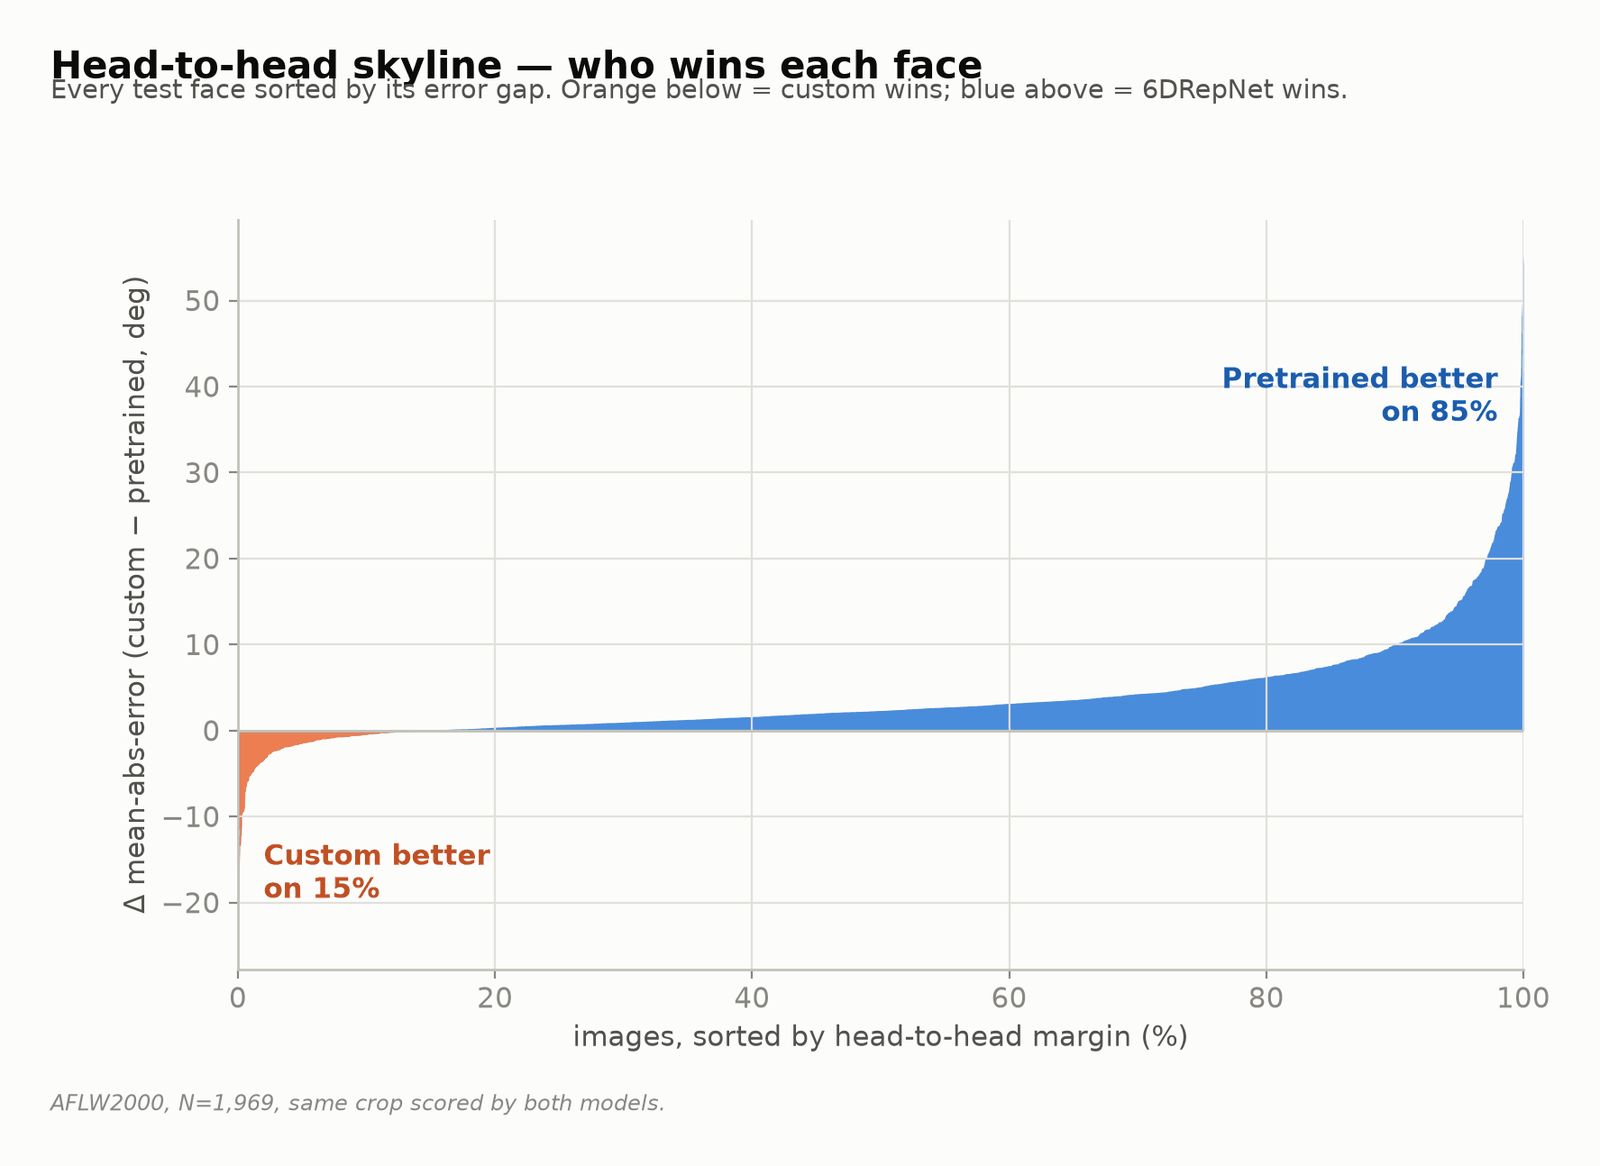
\includegraphics[width=\linewidth]{figures/headpose_H4_win_skyline.png}
\caption{Head-to-head skyline --- every AFLW2000 face sorted by its per-face error gap.}
\label{fig:22}
\end{figure}

Beyond the 14.58 \% win rate the extremes carry a caution. Catastrophic failures above 30$^{\circ}$ number 63 for the proposed network (3.20 \% of faces, contributing 1.36$^{\circ}$ of its 7.37$^{\circ}$ MAE) and 9 for the baseline (0.46 \%, 0.23$^{\circ}$ of 3.48$^{\circ}$). Their contribution to the aggregate is

\begin{equation}
\label{eq:239}
\begin{aligned}
\mathrm{contribution} = (1/n) \Sigma _{i \in \mathcal{C}} e(i) , \\
\mathcal{C} = { i : e(i) > 30^{\circ} } ,
\end{aligned}
\end{equation}

and excluding them leaves 6.01$^{\circ}$ against 3.25$^{\circ}$, so the gap is not outlier-driven. But the baseline's single worst error (119.6$^{\circ}$) \emph{exceeds} the proposed network's (92.6$^{\circ}$). The more accurate model owns the larger extreme, which argues against selecting architectures on maximum-error criteria over test sets of this size --- the maximum of n draws is an inconsistent statistic whose expectation grows with n for any heavy-tailed error law --- and which matters here because a single 90$^{\circ}$+ error inside a dwell window is exactly the event the 1,200 ms cooldown exists to contain.

\FIGREF{23} stratifies by yaw band, where the shrinkage account is directly testable.

\begin{figure}[pos=htbp]
\centering
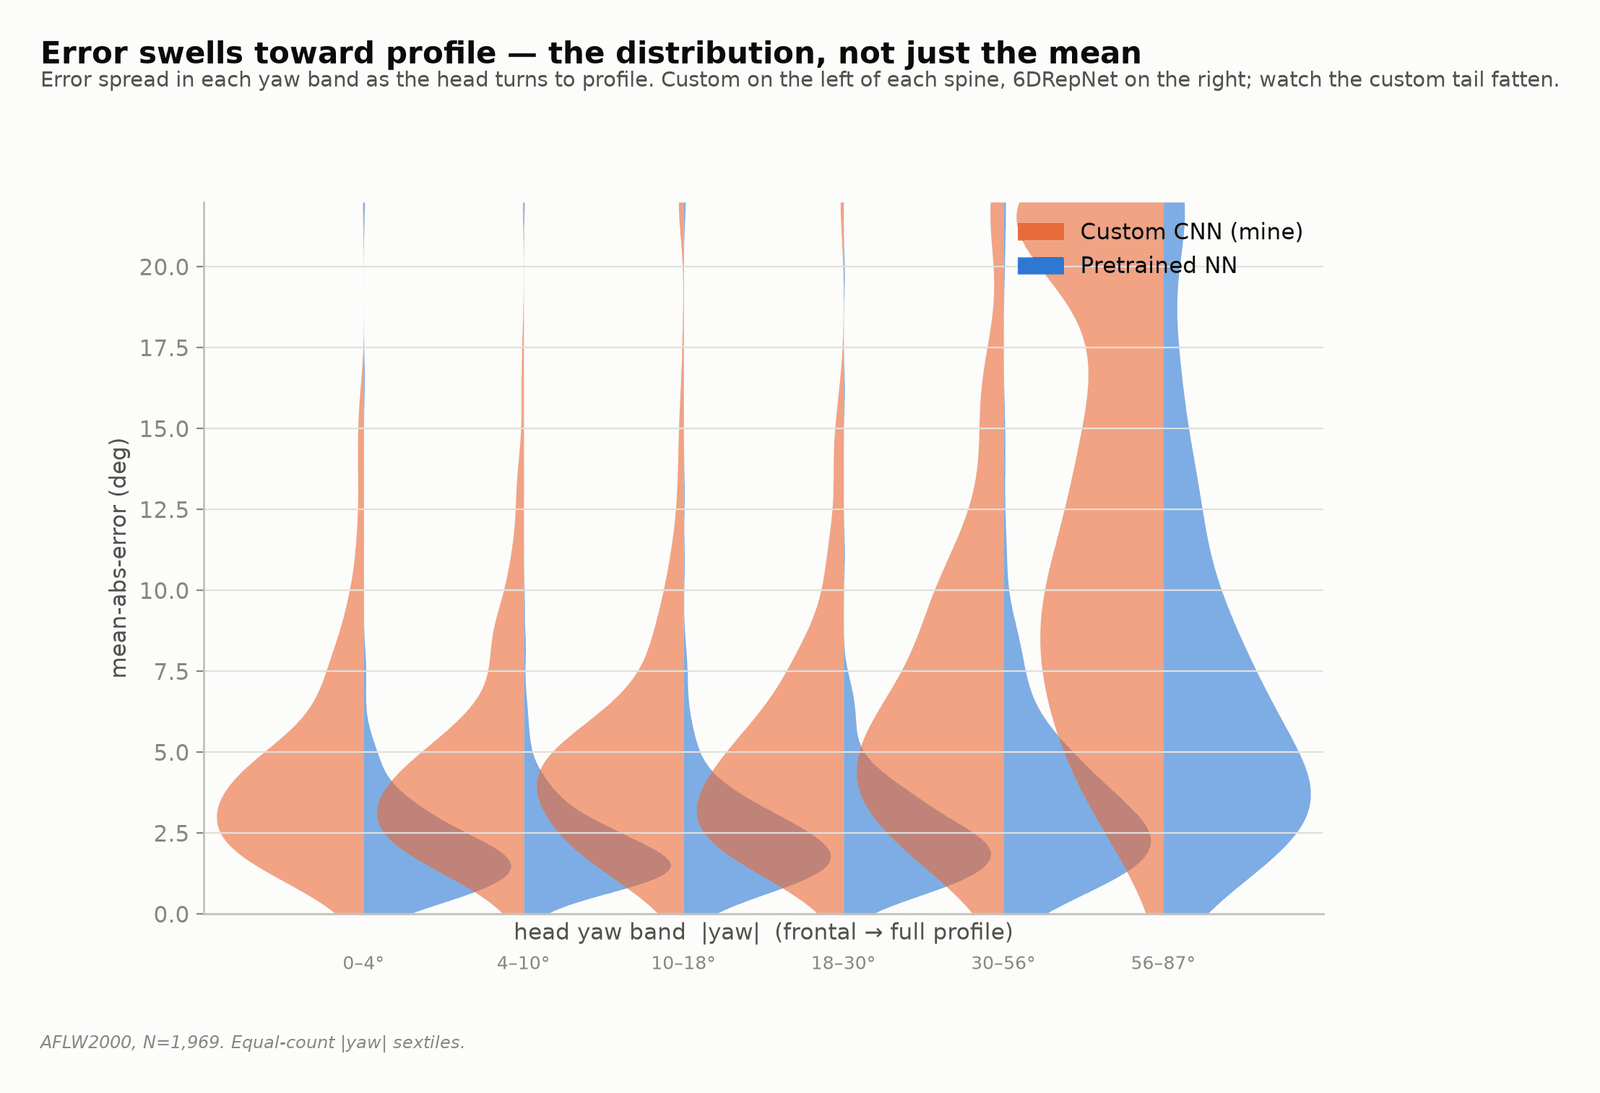
\includegraphics[width=\linewidth]{figures/headpose_H5_yaw_ridgeline.png}
\caption{Error versus profile --- error distributions per yaw band, from frontal through to full profile.}
\label{fig:23}
\end{figure}

Yaw-axis MAE runs 6.11$^{\circ}$, 6.98$^{\circ}$, 9.78$^{\circ}$ and 18.43$^{\circ}$ across the four bands, while the error predicted by gain deficiency alone,

\begin{equation}
\label{eq:240}
\hat{e}_{\mathrm{shrink}}(\text{band}) = ( 1 - \hat{s}_{\mathrm{yaw}} ) \cdot \mathbb{E}[ |\theta _{\mathrm{yaw}}| | \;\text{band} ] = 0.178 \cdot \mathbb{E}[ |\theta _{\mathrm{yaw}}| | \;\text{band} ] ,
\end{equation}

runs 1.13$^{\circ}$, 3.89$^{\circ}$, 7.99$^{\circ}$ and 12.64$^{\circ}$. The explained fraction

\begin{equation}
\label{eq:241}
\hat{e}_{\mathrm{shrink}} / e_{\mathrm{observed}} : 18 \% \to 56 \% \to 82 \% \to 69 \%
\end{equation}

rises from 18 \% of observed error at frontal to a dominant share beyond 30$^{\circ}$. Shrinkage is thus a minor contributor near frontal and the dominant one at profile, accounting for the accelerating degradation without any additional failure mechanism. The distributions broaden and shift together rather than becoming bimodal; bimodality would indicate sign confusion from flip augmentation without the label inversion of \EQREF{26}, and its absence confirms the augmentation logic is correct.

The deployment consequence is precise and follows from \EQREF{130}:

\begin{equation}
\label{eq:242}
\theta _{\mathrm{true}}^{\mathrm{trigger}} = \theta _{\mathrm{on}} / \hat{s}_{\mathrm{yaw}} = 30^{\circ} / 0.822 = 36.5^{\circ} ,
\end{equation}

so a user must turn to roughly 36.5$^{\circ}$ of true yaw to cross a 30$^{\circ}$ trigger. This is a systematic, stable and learnable offset --- users adapt to it within a session --- rather than an erratic one, which is why the gesture layer remains usable at an 8.74$^{\circ}$ yaw MAE.

\FIGREF{24} gives the regression fits.

\begin{figure}[pos=htbp]
\centering
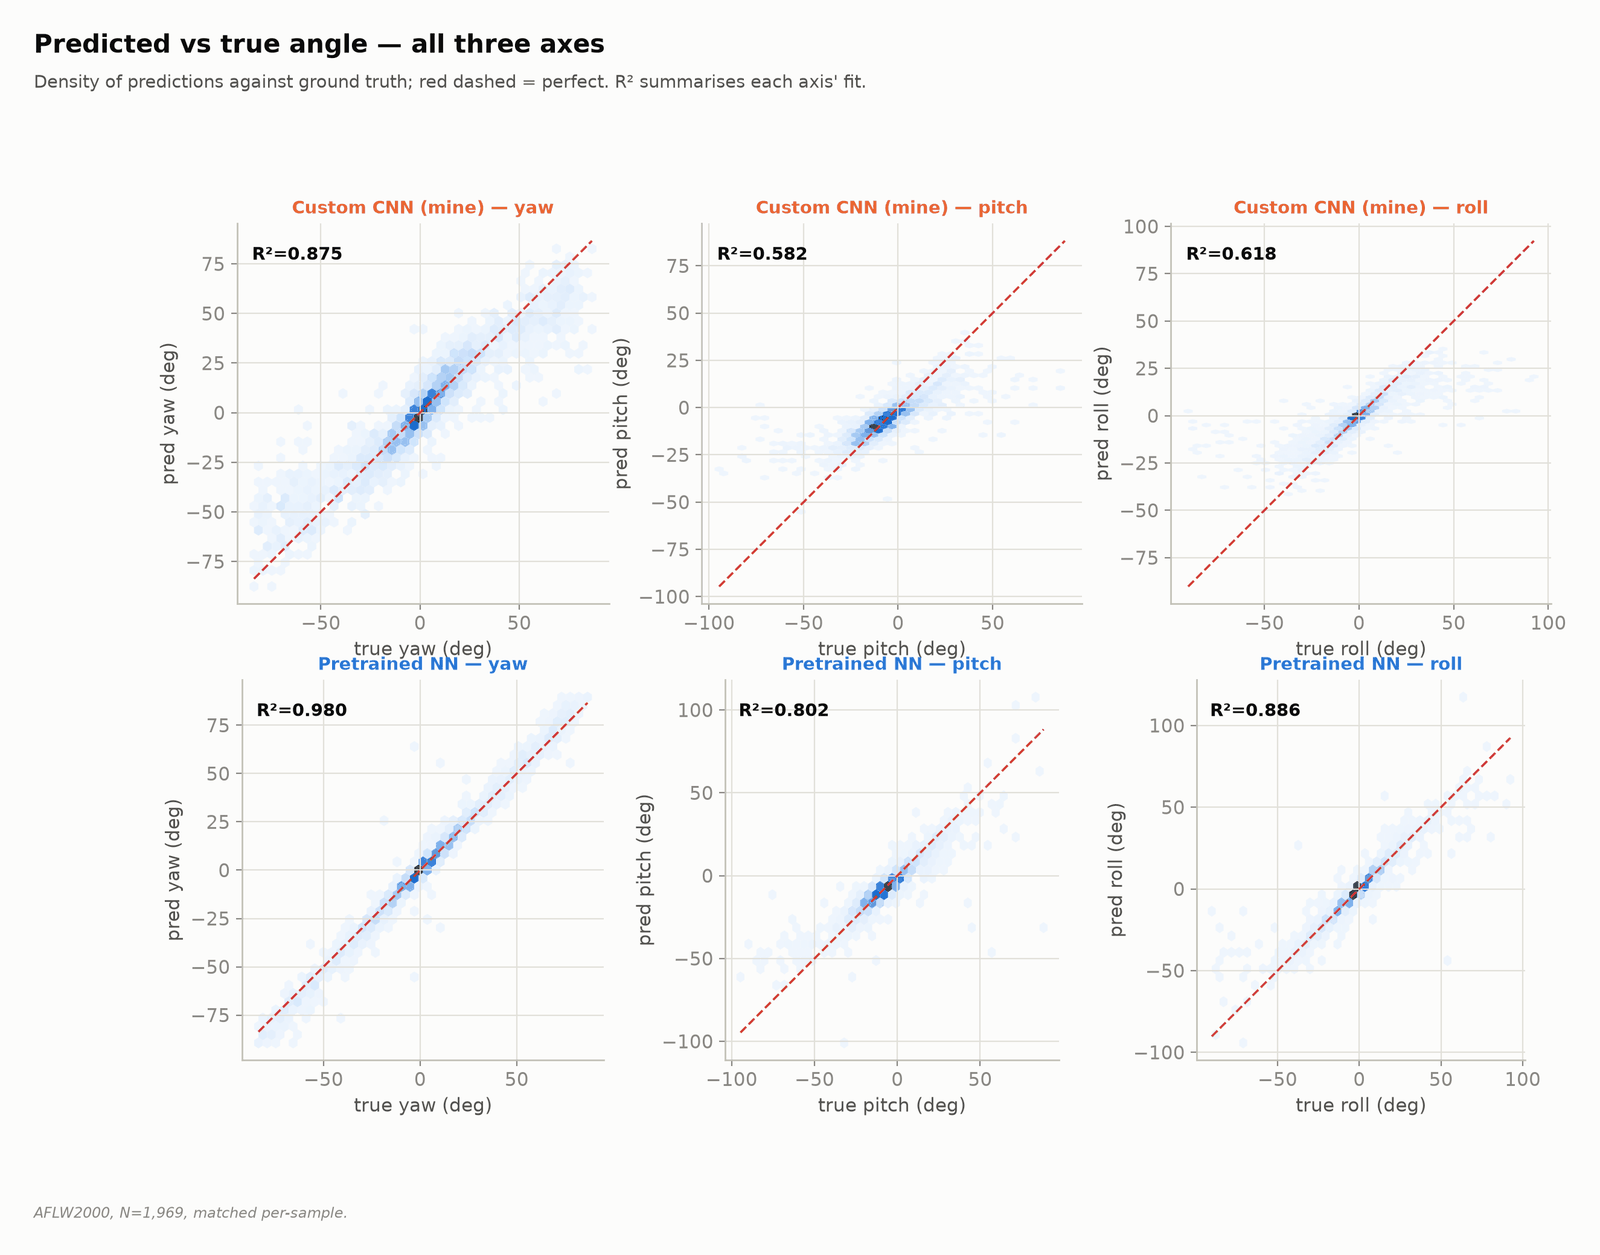
\includegraphics[width=\linewidth]{figures/headpose_H6_true_vs_pred.png}
\caption{Predicted versus true --- density-weighted fits with coefficient of determination for yaw, pitch and roll.}
\label{fig:24}
\end{figure}

Explained variance by \EQREF{153} is 87.5 \% for yaw, 61.8 \% for roll and 58.2 \% for pitch, against 98.0 \%, 88.6 \% and 80.2 \%. Read alongside the fitted slopes \EQREF{225} the two statistics separate cleanly: R$^{2}$ measures how much structure the network recovers, the slope whether it recovers it at the correct scale. Formally, by \EQREF{212} the two are related through

\begin{equation}
\label{eq:243}
R^{2} = \hat{s}^{2} \sigma _{\theta} ^{2} / ( \hat{s}^{2} \sigma _{\theta} ^{2} + \sigma _{\zeta} ^{2} ) ,
\end{equation}

so a high R$^{2}$ with a low $\hat{s}$ is the signature of \emph{low residual variance at contracted scale} --- the profile of an under-confident rather than an uninformed estimator. The proposed network scores comparatively well on the first and poorly on the second, and that is the reason a fixed trigger threshold rather than a learned one remains adequate: an under-confident estimator's output is a deterministic rescaling of the truth, which a fixed threshold accommodates by \EQREF{242}.

\FIGREF{25} locates the winner in pose space.

\begin{figure}[pos=htbp]
\centering
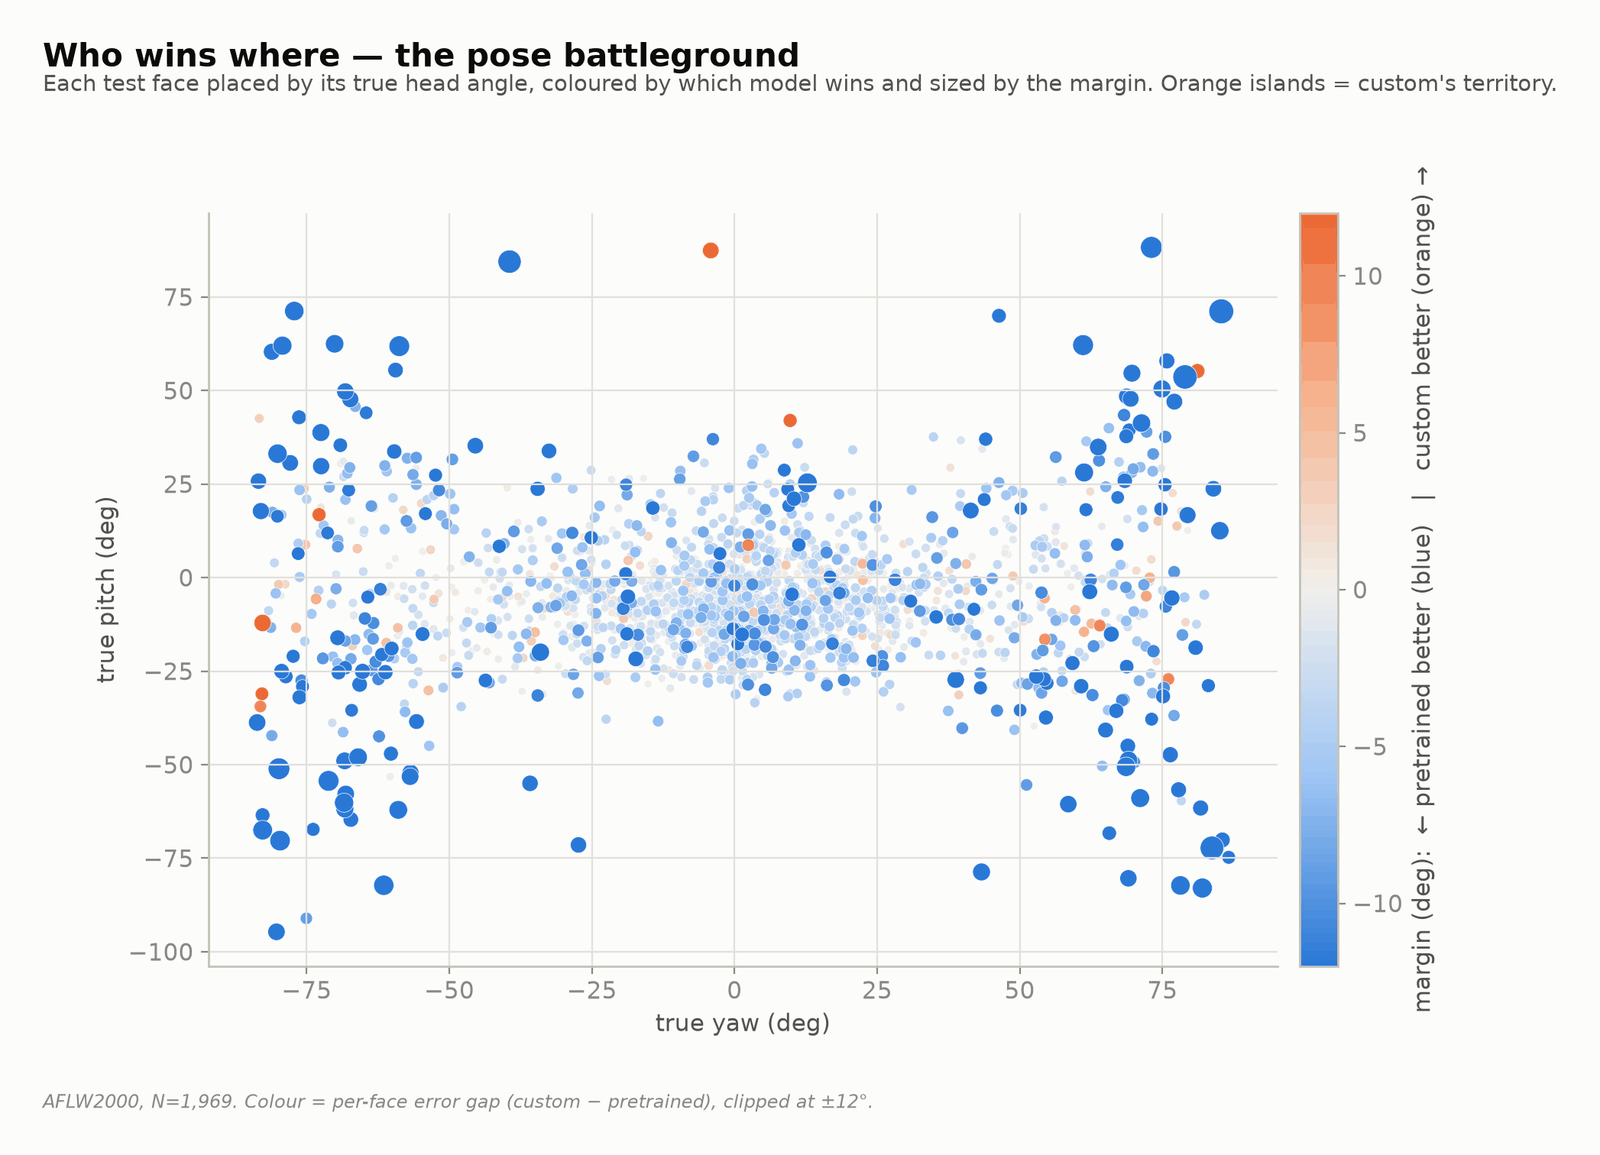
\includegraphics[width=\linewidth]{figures/headpose_H7_win_map.png}
\caption{Pose battleground --- every face placed at its true angle and coloured by which model achieves the lower error.}
\label{fig:25}
\end{figure}

Winning regions interleave rather than separating territorially, exactly as constant-ratio degradation predicts: with no pose region of systematic advantage, the wins are per-sample noise inside a dominated comparison. A pose-conditioned switching policy --- superficially attractive as a route to baseline accuracy at reduced average cost --- has no support here, and the $r_{\mathrm{AR}}$ = 0.671 error correlation independently confirms it would have little to exploit, since by \EQREF{164} the achievable gain is bounded by 7.5 \% even with an oracle.

\FIGRANGE{26}{29} re-render the same data as continuous fields, testing the joint claims of constant ratio, zero bias and benchmark sparsity.

\begin{figure}[pos=htbp]
\centering
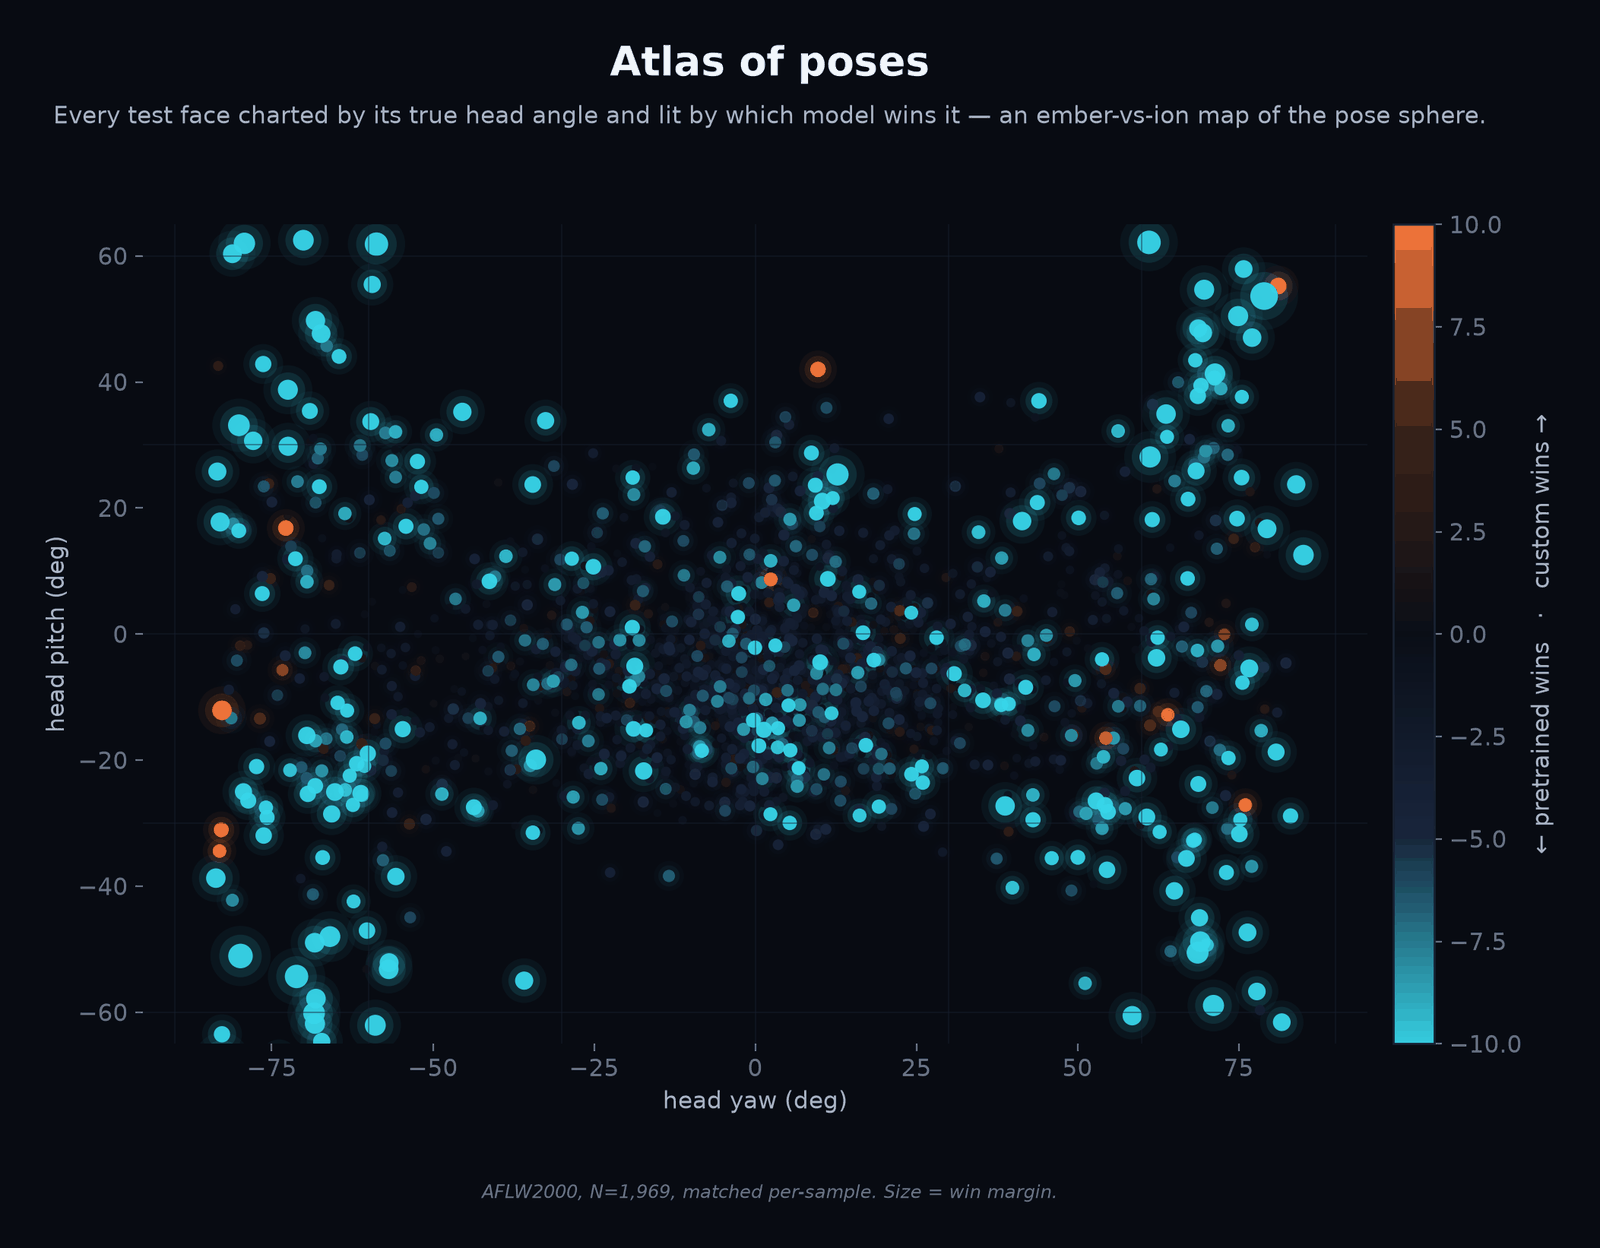
\includegraphics[width=\linewidth]{figures/figures_art_headpose_HA1_atlas.png}
\caption{Atlas of poses --- every AFLW2000 face charted at its true head angle and lit according to which model achieves the lower error.}
\label{fig:26}
\end{figure}

The continuous counterpart of \FIGREF{25} makes the absence of territory explicit: the 14.58 \% of faces won scatter with no contiguous region of advantage. Under a 2.03--2.21$\times$ ratio across the manifold by \EQREF{237}, scattered wins are what per-sample noise in a dominated comparison produces, and the $r_{\mathrm{AR}}$ = 0.671 correlation confirms the two models fail on the same faces. Two independent measurements --- one spatial, one rank-based --- converge on the same conclusion about fusion.

\begin{figure}[pos=htbp]
\centering
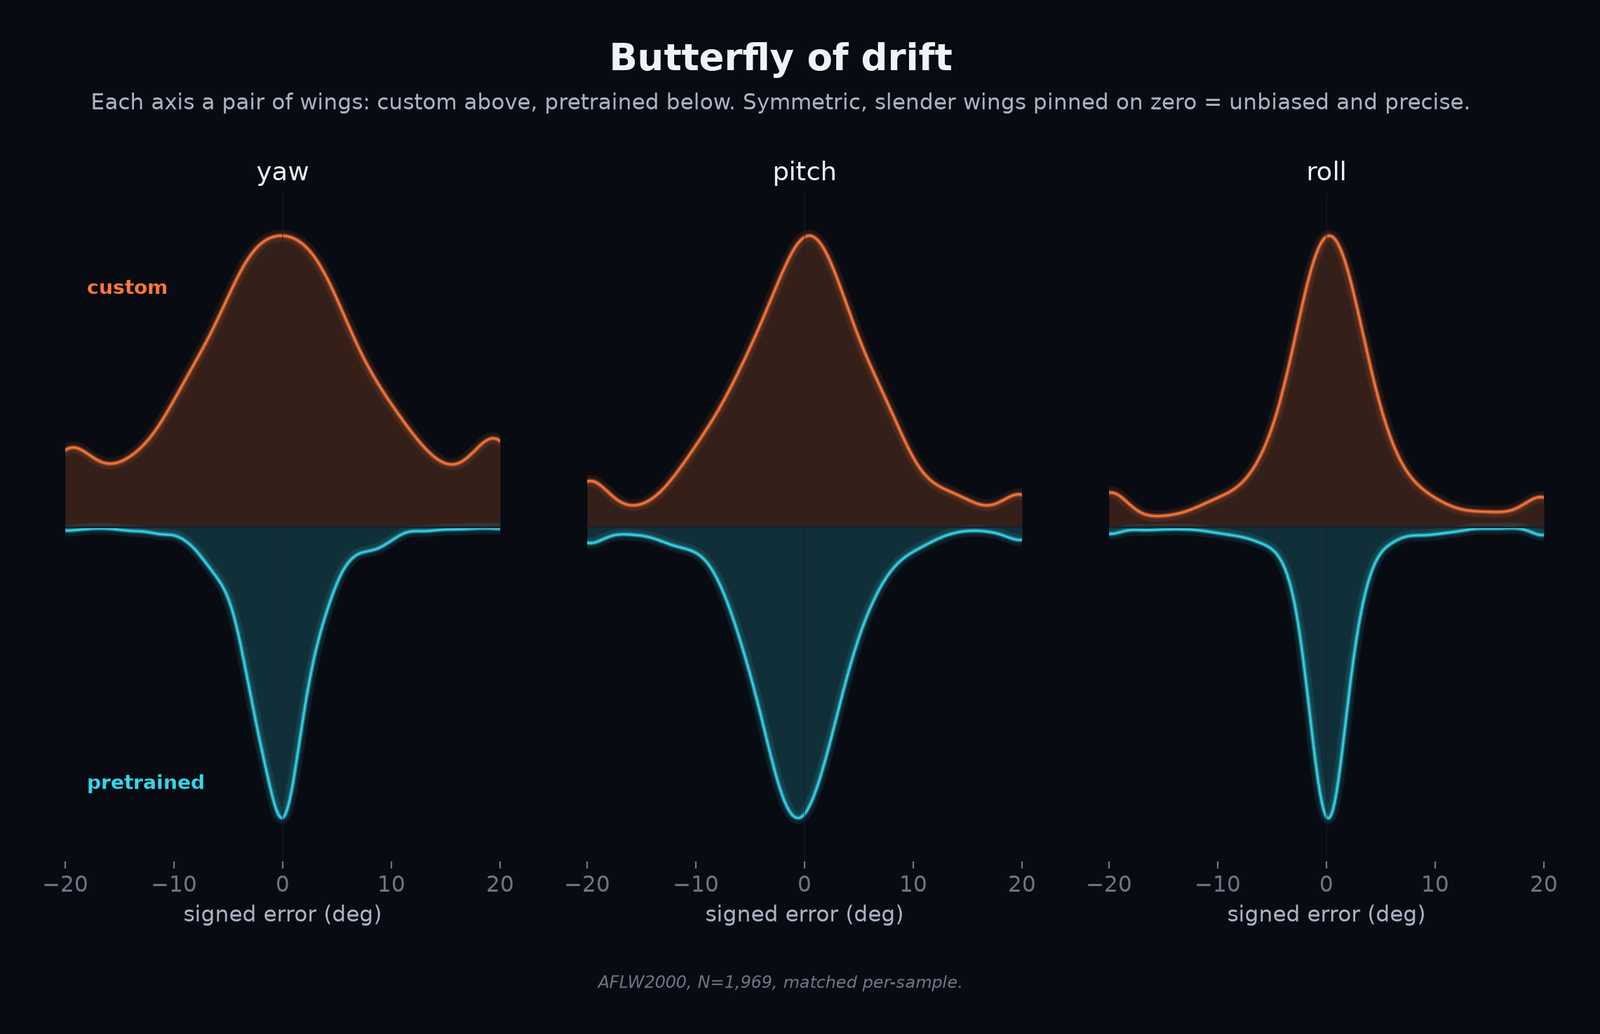
\includegraphics[width=\linewidth]{figures/figures_art_headpose_HA2_butterfly.png}
\caption{Butterfly of drift --- per-axis signed-error distributions, proposed network as the upper wing and the pretrained baseline as the lower wing of each pair.}
\label{fig:27}
\end{figure}

Every wing is pinned on zero by \EQREF{229}, so the deficit is width, not displacement. Spread ratios are

\begin{equation}
\label{eq:244}
\begin{aligned}
\sigma ^A/\sigma ^R: 2.49\times (\text{yaw}) , 1.46\times (\text{pitch}) , \\
1.84\times (\text{roll}) .
\end{aligned}
\end{equation}

That the yaw ratio is largest while yaw is also the best-explained (R$^{2}$ = 0.875) and least contracted ($\hat{s}$ = 0.822) axis is the visual statement of the units artefact of \EQREF{234} --- a modest relative deficit over a wide range produces the widest absolute distribution. The pinning on zero is what licenses the dwell-averaging argument of \EQREF{230}--\EQREF{231}.

\begin{figure}[pos=htbp]
\centering
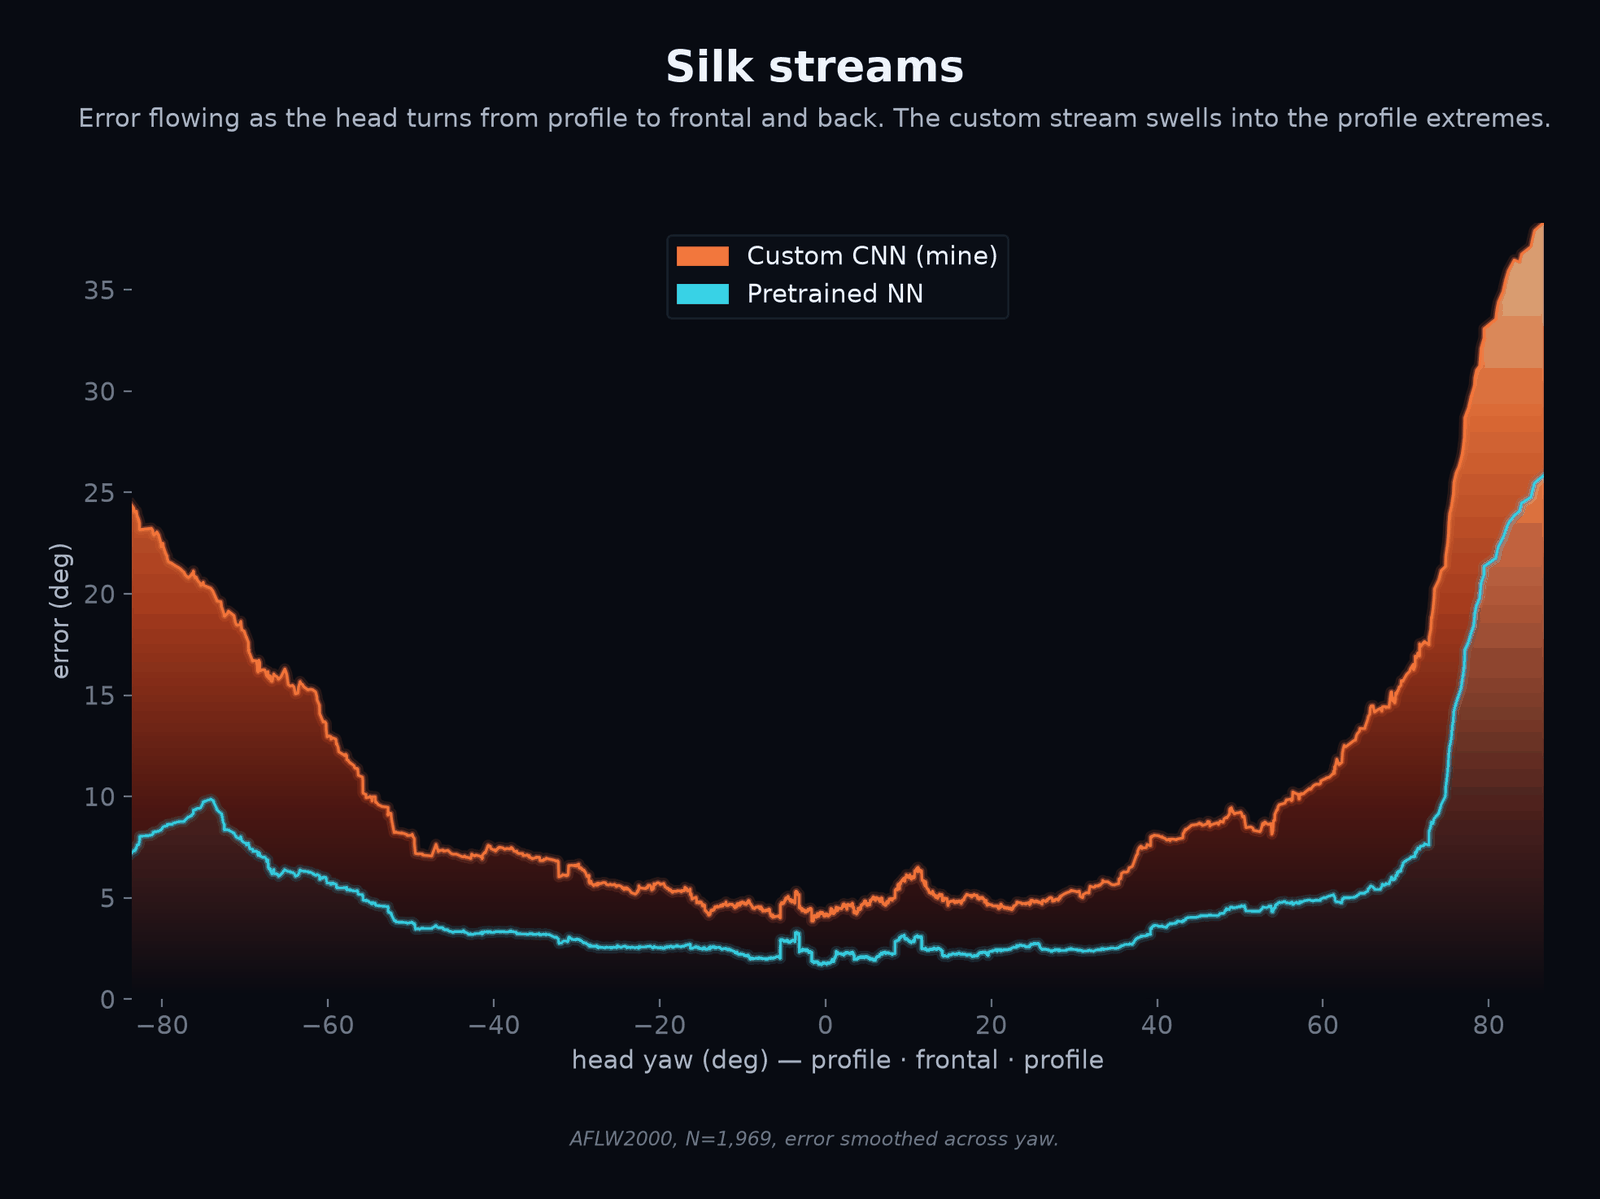
\includegraphics[width=\linewidth]{figures/figures_art_headpose_HA3_silk.png}
\caption{Silk streams --- error flowing as a continuous function of head rotation, from full profile through frontal and back.}
\label{fig:28}
\end{figure}

Continuity is the finding: the stream swells smoothly from 4.77$^{\circ}$ at frontal to 18.16$^{\circ}$ beyond 60$^{\circ}$ with no discontinuity or bifurcation, so the progressively occluded operator identified in \FIGREF{31} below degrades gracefully rather than failing abruptly. A discontinuity would signal a regime change, a bifurcation sign confusion; neither appears. Graceful degradation is what permits the gesture layer to stay stable at large angles, because error grows predictably with a state the state machine already tracks.

\begin{figure}[pos=htbp]
\centering
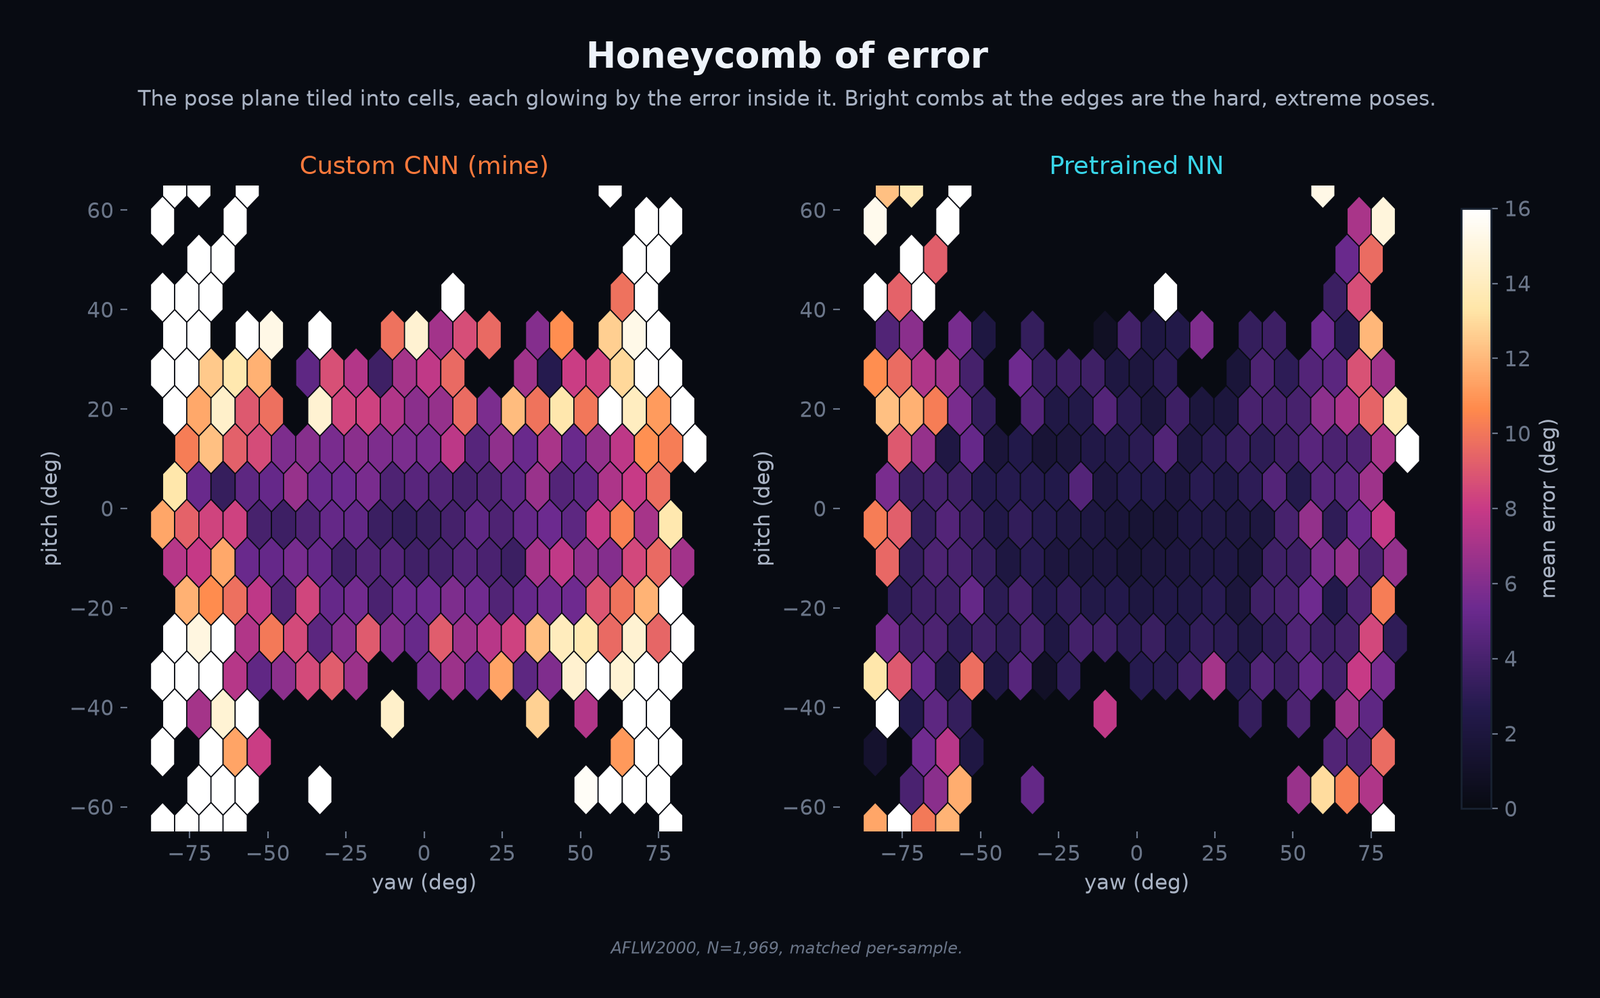
\includegraphics[width=\linewidth]{figures/figures_art_headpose_HA4_honeycomb.png}
\caption{Honeycomb of error --- the yaw $\times$ pitch plane tiled into cells, each glowing according to the mean error of the faces it contains.}
\label{fig:29}
\end{figure}

Tiling restores what smooth interpolation suppresses: cell occupancy. The brightest peripheral cells are the sparsest --- 278 of 1,969 faces lie beyond 60$^{\circ}$ of yaw against 891 within 15$^{\circ}$ --- so extreme-pose estimates rest on roughly a seventh of the evidence supporting frontal ones. The standard error of a band mean scales as

\begin{equation}
\label{eq:245}
\begin{aligned}
SE(\text{band}) = \sigma _{\mathrm{band}} / \sqrt{n}_{\mathrm{band}} , \\
SE(>60^{\circ})/SE(<15^{\circ}) = ( \sigma _{>60}/\sigma _{<15} ) \cdot \sqrt{891/278} \approx 1.79 \cdot ( \sigma \;\text{ratio} ) ,
\end{aligned}
\end{equation}

so the region where the models differ most is the region the benchmark constrains least, and the 18.16$^{\circ}$ against 8.20$^{\circ}$ comparison there carries materially wider uncertainty than its frontal counterpart. This caveat applies to AFLW2000-based comparisons generally, and it is reassuring for this system only because the operative range lies inside the well-populated bands.

\subsubsection{What the network computes}

\begin{figure}[pos=htbp]
\centering
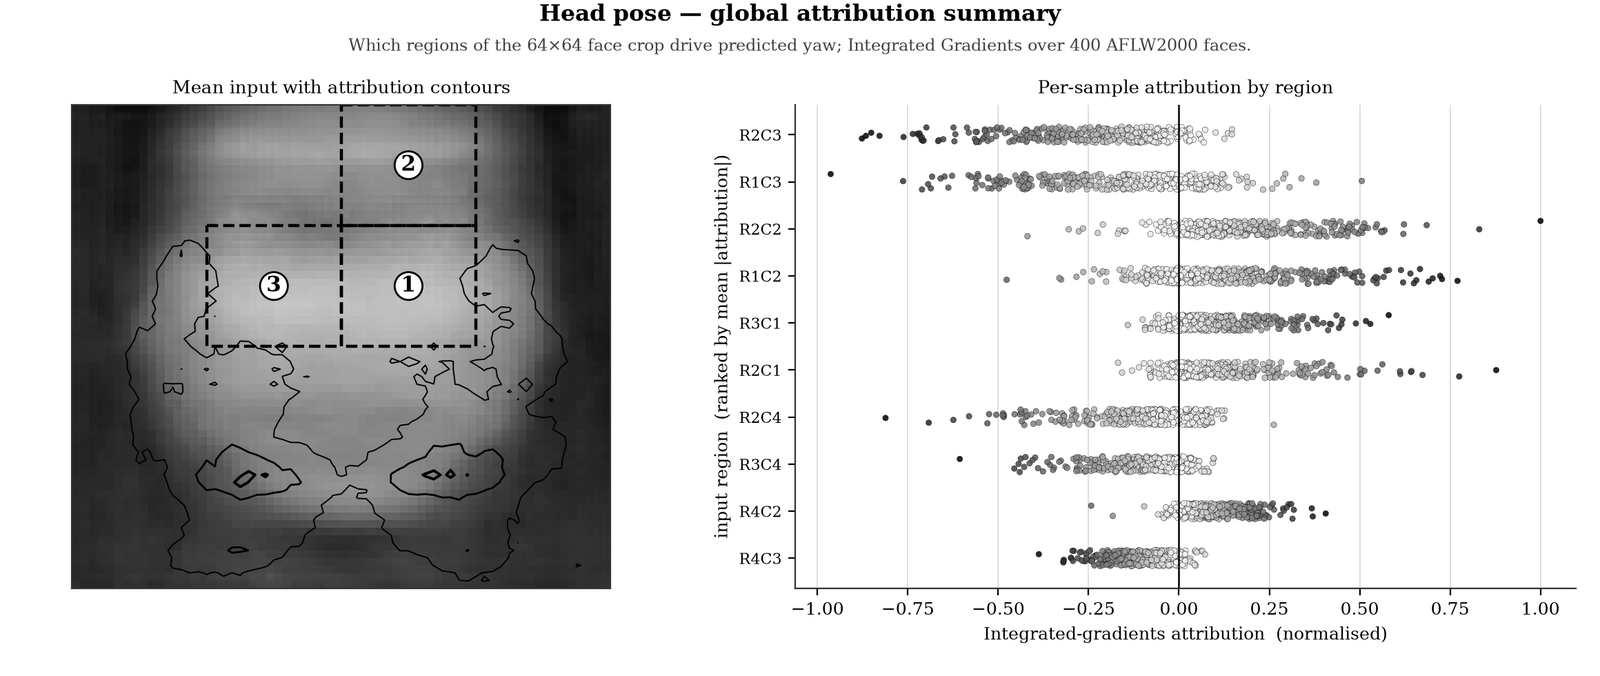
\includegraphics[width=\linewidth]{figures/attribution_headpose_A1_summary.png}
\caption{Head pose --- global attribution summary for predicted yaw over the 64 $\times$ 64 face crop.}
\label{fig:30}
\end{figure}

The attribution field is antisymmetric about the facial midline: columns 1--2 predominantly positive (R2C2, R1C2, R3C1, R2C1), columns 3--4 predominantly negative (R2C3, R1C3, R2C4, R3C4), with mass in the brow--eye--nose band of rows 1--3. Formally, writing the region attribution vector as a function of the mirror operator $\mathcal{M}$,

\begin{equation}
\label{eq:246}
\mathrm{Attr}( \mathcal{M} R_k ; x ) \approx - \mathrm{Attr}( R_k ; x ) \;\text{for k in the brow}\;--\;\text{eye}\;--\;\text{nose band} ,
\end{equation}

which is precisely the antisymmetric operator \EQREF{216} already identified for gaze. Yaw is physically encoded by the left--right asymmetry of that band under projection, and the network recovered exactly that computation --- structurally the same class of operator the gaze network learned, which is why both exhibit the same shrinkage behaviour: a differential operator's output amplitude falls as one of its two arguments is occluded, and \EQREF{155} then contracts the estimate. Row 4, jaw and chin, contributes little, a sensible allocation given it is the region most degraded by self-occlusion at profile.

\begin{figure}[pos=htbp]
\centering
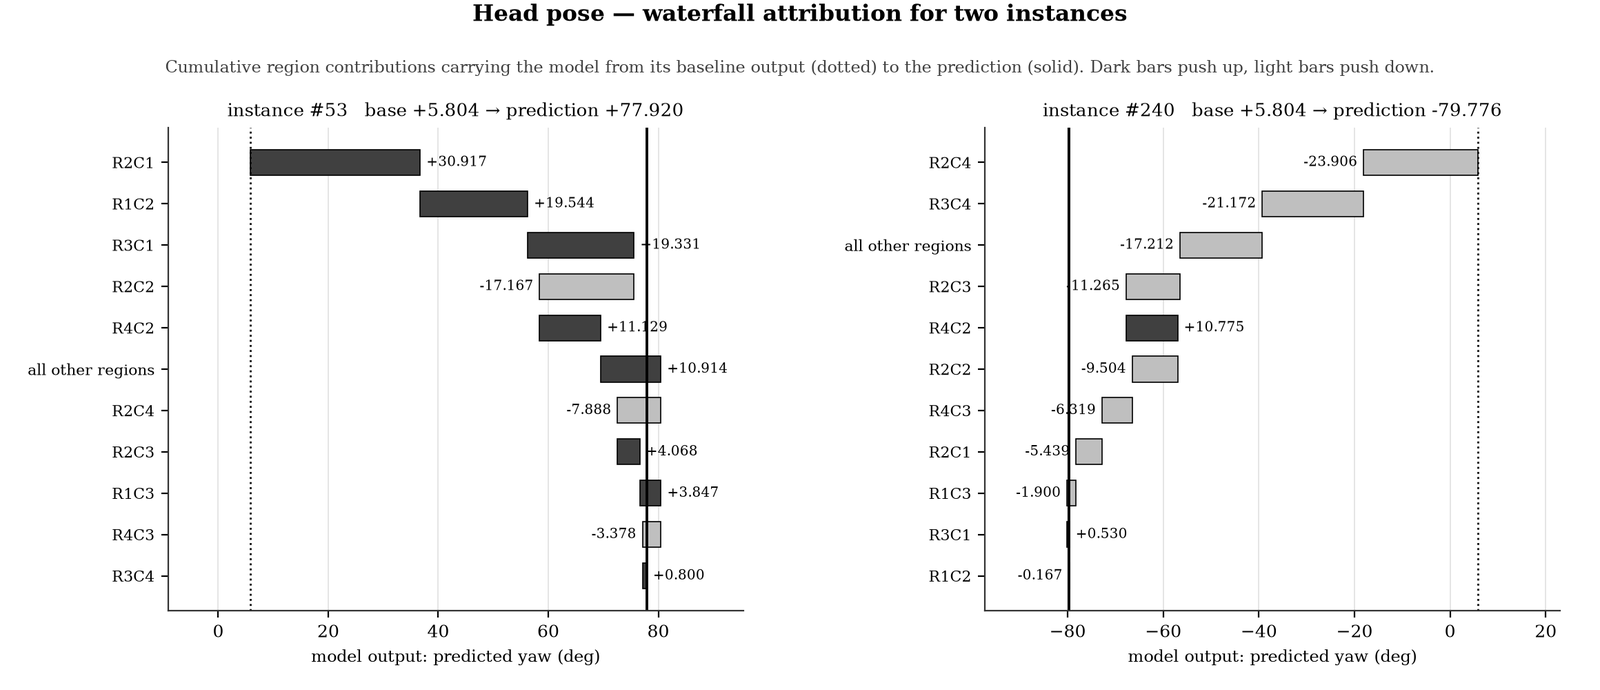
\includegraphics[width=\linewidth]{figures/attribution_headpose_A2_waterfall.png}
\caption{Head pose --- waterfall attribution for two extreme instances of predicted yaw.}
\label{fig:31}
\end{figure}

At extreme yaw the decomposition is dominated by one side of the antisymmetric pair, the occluded side contributing little. This is the mechanism generating the gain deficit of \FIGREF{23}. Modelling the differential operator's effective gain as a function of the visible fraction v($\theta_{\mathrm{yaw}}$) $\in$ [0,1] of the occluded hemiface,

\begin{equation}
\label{eq:247}
\begin{aligned}
s_{\mathrm{eff}}( \theta _{\mathrm{yaw}} ) = \sigma _{\theta} ^{2} / ( \sigma _{\theta} ^{2} + \sigma _{\varepsilon} ^{2}/v(\theta _{\mathrm{yaw}}) ) , \\
v \;\text{decreasing in}\; |\theta _{\mathrm{yaw}}| ,
\end{aligned}
\end{equation}

so that as yaw increases, half the differential measurement is lost to self-occlusion, effective gain falls, and the estimate compresses toward the frontal prior. Equation \EQREF{247} explains why contraction \emph{worsens with angle} rather than staying constant, matching the accelerating explained fraction of \EQREF{241}, and why no bimodality appears --- the operator degrades continuously rather than switching sign.

\begin{figure}[pos=htbp]
\centering
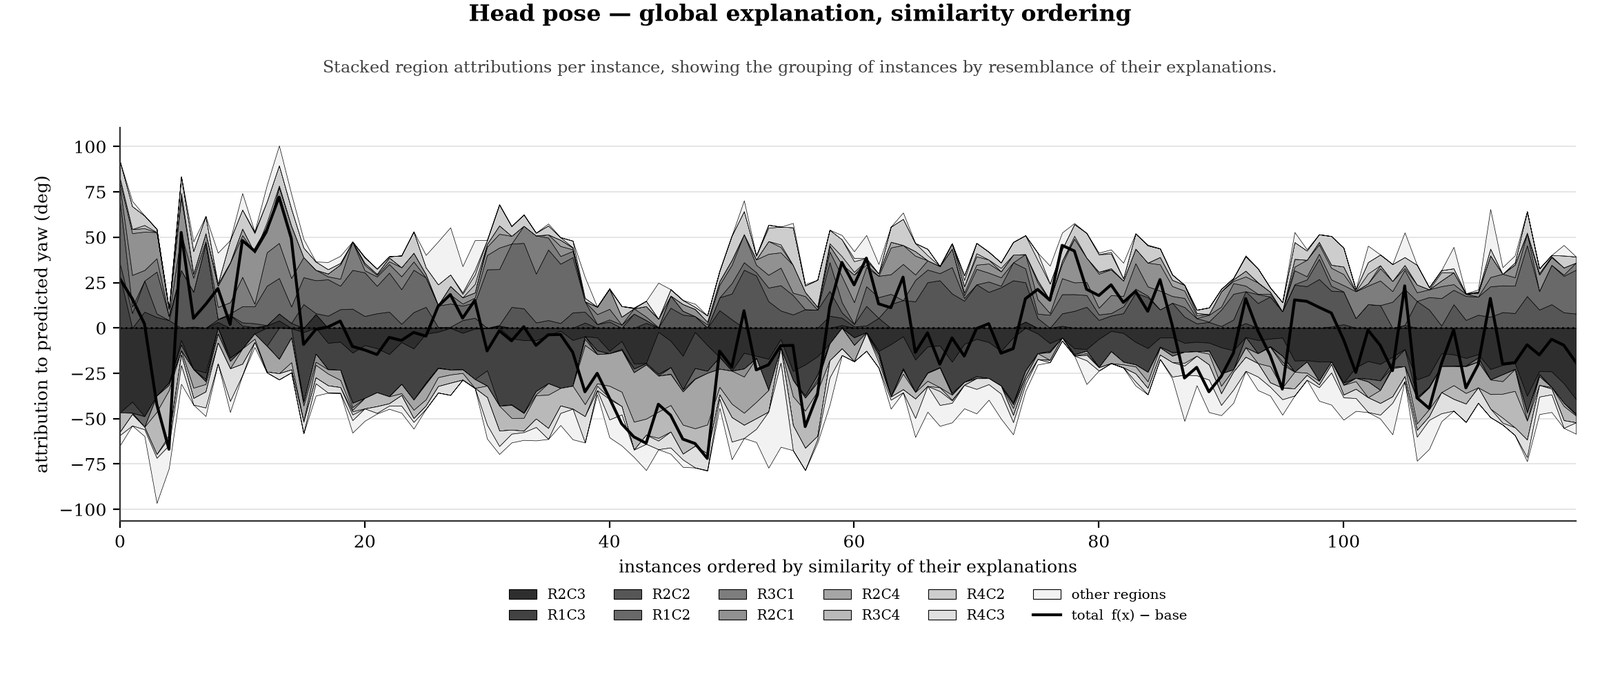
\includegraphics[width=\linewidth]{figures/attribution_headpose_A3_similarity.png}
\caption{Head pose --- global explanation under similarity ordering.}
\label{fig:32}
\end{figure}

Similarity ordering traces a smooth monotone progression of region weights following the pose manifold. No discontinuity appears anywhere along it, corroborating the constant-ratio degradation of \FIGREF{21} from an entirely independent measurement: there is no pose regime in which the network engages a qualitatively different strategy, only one in which the same strategy has less evidence available --- which is exactly the content of \EQREF{247}.

\begin{figure}[pos=htbp]
\centering
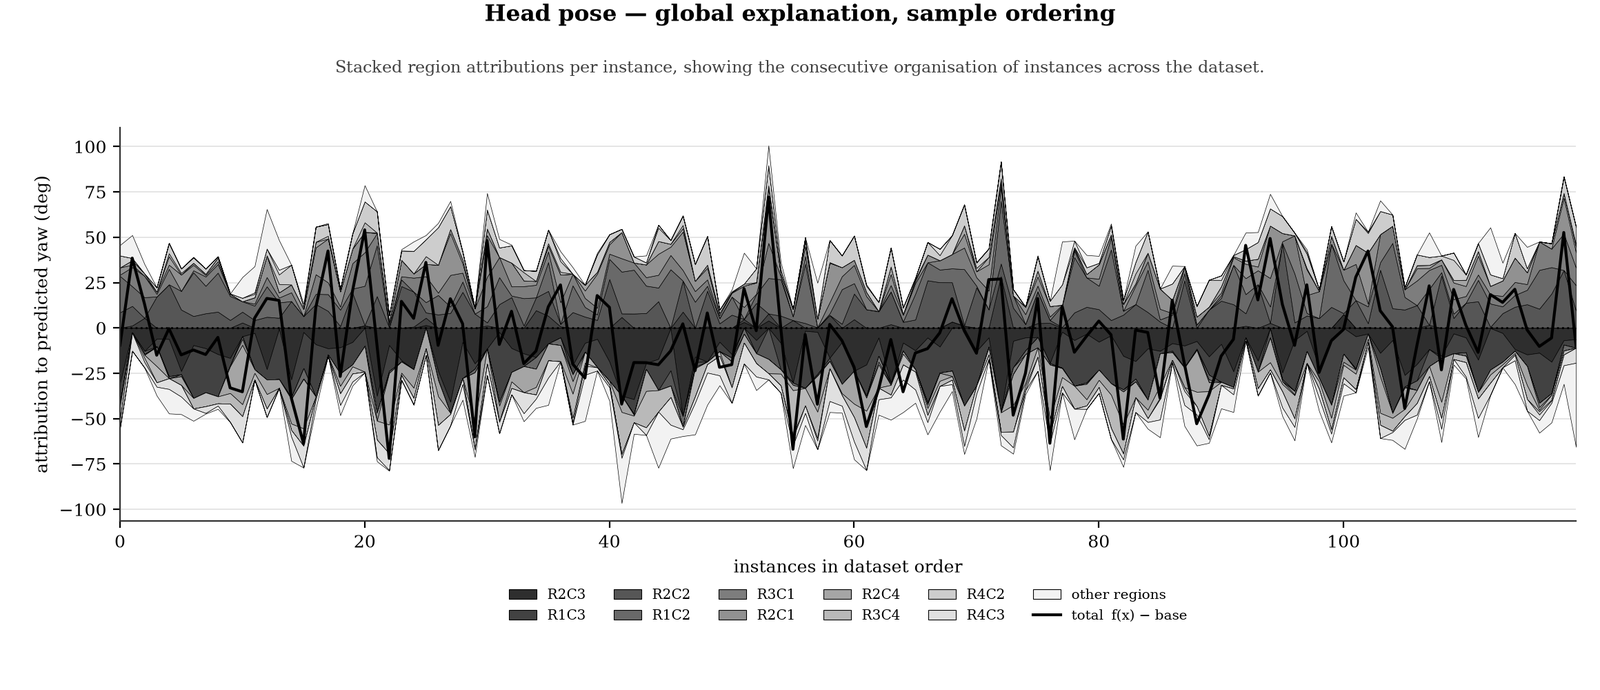
\includegraphics[width=\linewidth]{figures/attribution_headpose_A4_ordering.png}
\caption{Head pose --- global explanation under dataset ordering over AFLW2000.}
\label{fig:33}
\end{figure}

In dataset order the pattern is heterogeneous, reflecting AFLW2000's unordered pose composition. The absence of structure is the intended control: it confirms the coherent progression under similarity ordering in \FIGREF{32} is a property of the explanation manifold rather than an artefact of acquisition sequence, a distinction a single ordering could not have drawn.

\FloatBarrier

\subsection{Voice --- command execution}

Voice runs on its own audio thread, outside the camera loop's frame budget \EQREF{3}, and maps six keywords to the commands that make the rest of the interface operable: \emph{up} and \emph{down} scroll, \emph{stop} and \emph{go} pause and resume control, \emph{yes} and \emph{no} confirm and cancel. Its row in \TABREF{6} names per-class precision on the safety-critical words as the governing statistic, and the reason is consequence rather than frequency --- by \EQREF{135}, \emph{go} is the only route back once \emph{stop} has paused the system, so an error on it must be recovered by repetition against a system that is deliberately not acting. This section therefore reports per-class behaviour before aggregate behaviour, inverting the usual order.

On the 2,468-clip official test split the proposed network attains

\begin{equation}
\label{eq:248}
\begin{aligned}
\mathrm{Acc} = 94.53 \% , \mathrm{BalAcc} = 94.48 \% , \\
\;\text{macro}\;-F_{1} = 94.48 \% , \mathrm{MCC} = 0.9344 , \kappa = 0.9344 ,
\end{aligned}
\end{equation}

against the production ASR baseline at 95.50 \% accuracy and 97.43 \% macro-F$_{1}$. The 2.95 pp macro-F$_{1}$ gap is produced by a \emph{mechanism} rather than by discriminative superiority, and separating the two is the substance of this section.

\FIGREF{34} presents the error structure.

\begin{figure}[pos=htbp]
\centering
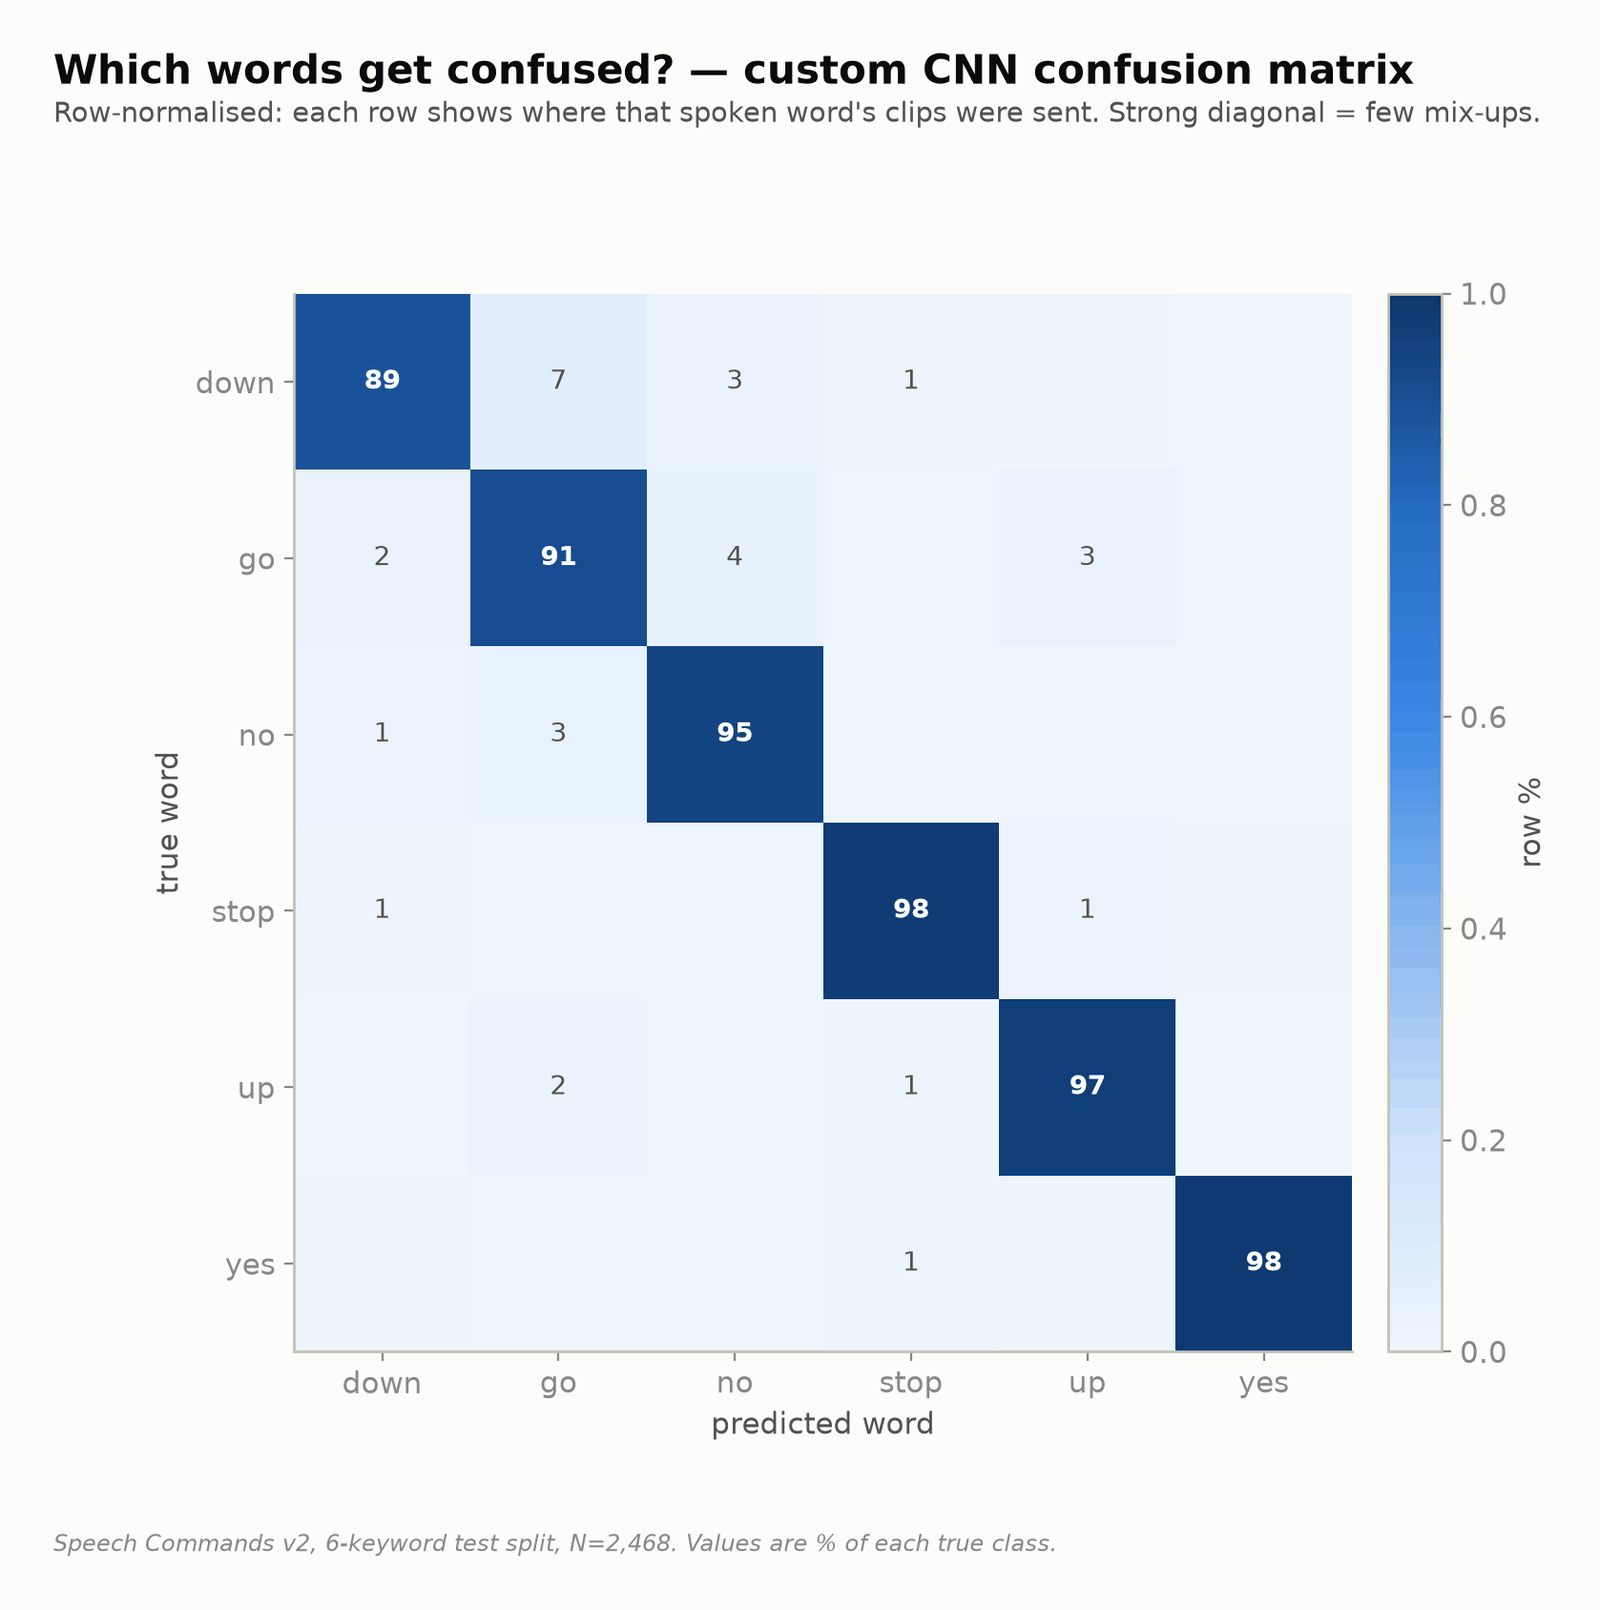
\includegraphics[width=\linewidth]{figures/voice_V1_confusion.png}
\caption{Confusion matrix --- row-normalised, showing where the clips of each spoken keyword were assigned.}
\label{fig:34}
\end{figure}

The 135 errors concentrate in three pairs: \emph{down} $\leftrightarrow$ \emph{go} (38 clips), \emph{go} $\leftrightarrow$ \emph{no} \EQREF{30} and \emph{down} $\leftrightarrow$ \emph{no} \EQREF{17}, together

\begin{equation}
\label{eq:249}
( 38 + 30 + 17 ) / 135 = 63.0 \%
\end{equation}

of all errors. All three involve a back rounded nucleus and differ principally in a brief initial consonant, so the discriminative evidence occupies a few tens of milliseconds at onset --- a small number of the T = 81 time frames produced by \EQREF{28}. The precision--recall split localises the mechanism:

\begin{equation}
\label{eq:250}
\begin{aligned}
\mathrm{Prec}(go) = 0.877 , \\
\mathrm{Rec}(go) = 0.908 ; \mathrm{Prec}(\text{down}) = 0.948 , \\
\mathrm{Rec}(\text{down}) = 0.889 .
\end{aligned}
\end{equation}

Since Prec(go) < Rec(go) while the reverse holds for \emph{down}, \emph{go} is an \textbf{attractor}: it absorbs clips from its phonetic neighbours rather than being a class the network fails to recognise. Formally, writing N(c'$\to$c) for the count of true-c' clips assigned to c, the in-flow/out-flow imbalance

\begin{equation}
\label{eq:251}
\Lambda _c = \Sigma _{c' \neq c} N_{c'\to c} - \Sigma _{c' \neq c} N_{c\to c'}
\end{equation}

is positive for \emph{go} and negative for \emph{down}, which is the quantitative content of ``attractor''.

For the interface this is the most consequential single result in the voice evaluation, and it is a \textbf{design fault rather than a model fault}. \emph{go} is bound to ``resume control'': the command that reactivates the interface after \emph{stop} has suspended it. Its being an attractor means spurious resumes while the system is deliberately paused; its 0.877 precision is the worst in the vocabulary; and its partners in confusion are \emph{down} (scroll) and \emph{no} (escape), both frequently spoken. Meanwhile \emph{stop}, the pause direction, is among the strongest words (precision 0.971, recall 0.976). The safety-critical asymmetry therefore runs the wrong way --- the gate is easy to close and easy to open accidentally --- and the remedy costs nothing: rebinding ``resume control'' to a phonetically distant token, one with fricative or stop-cluster onset (the acoustic class that \FIGREF{37} below shows the network separates best), removes the largest error mode without retraining a single parameter.

\FIGREF{35} places the proposed network against the ASR baseline across shared metrics.

\begin{figure}[pos=htbp]
\centering
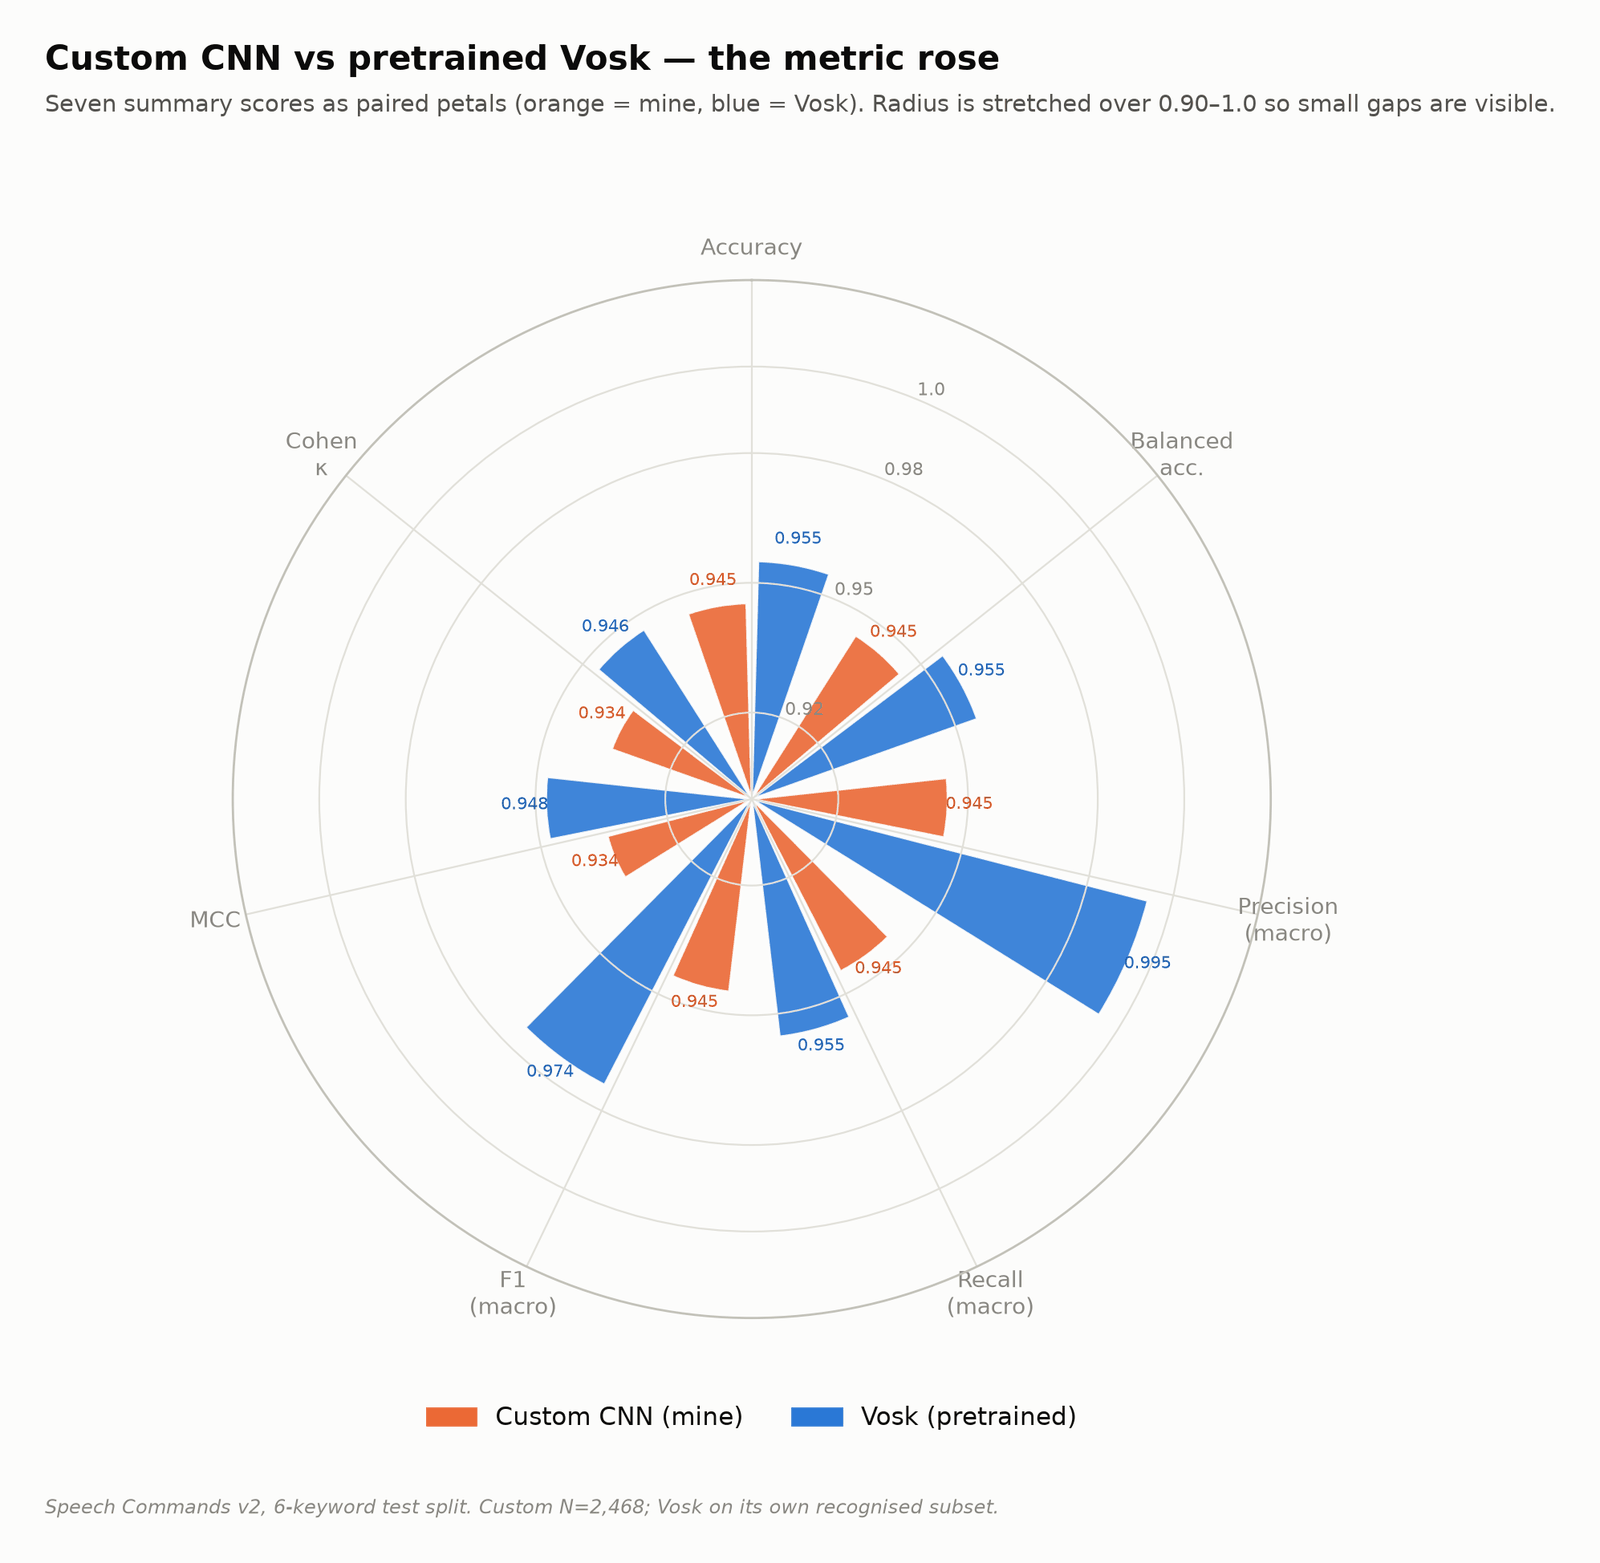
\includegraphics[width=\linewidth]{figures/voice_V2_metric_rose.png}
\caption{Metric rose --- seven summary scores as paired petals, proposed network against the pretrained ASR baseline.}
\label{fig:35}
\end{figure}

The baseline's macro precision is 99.45 \% against 94.53 \% while its macro recall is 95.53 \% against 94.48 \%, and the divergence is explained entirely by abstention. The engine rejects 98 of 2,468 clips, emitting no hypothesis, and among the 2,370 it does transcribe it commits only 13 substitutions:

\begin{equation}
\label{eq:252}
\mathrm{cov}_R = 2370/2468 = 96.03 \% , \mathrm{risk}_R = 13/2370 = 0.55 \% .
\end{equation}

It is not a more discriminative classifier but one equipped with a rejection option in the sense of \EQREF{132}, converting would-be substitutions into non-responses. Macro-F$_{1}$ rewards this --- abstention costs recall but protects precision --- whereas forced-choice accuracy, the like-for-like comparison under \EQREF{131}, differs by only

\begin{equation}
\label{eq:253}
95.50 \% - 94.53 \% = 0.97 pp .
\end{equation}

In this interface the distinction is operational rather than semantic: under the asymmetric loss \EQREF{134} a substitution executes an unintended command while an abstention costs one repetition, and given the \emph{go} binding above the abstention is clearly preferable.

\FIGREF{36} asks whether the same rejection regime is available to the proposed network, which requires its confidence to be a probability rather than a ranking.

\begin{figure}[pos=htbp]
\centering
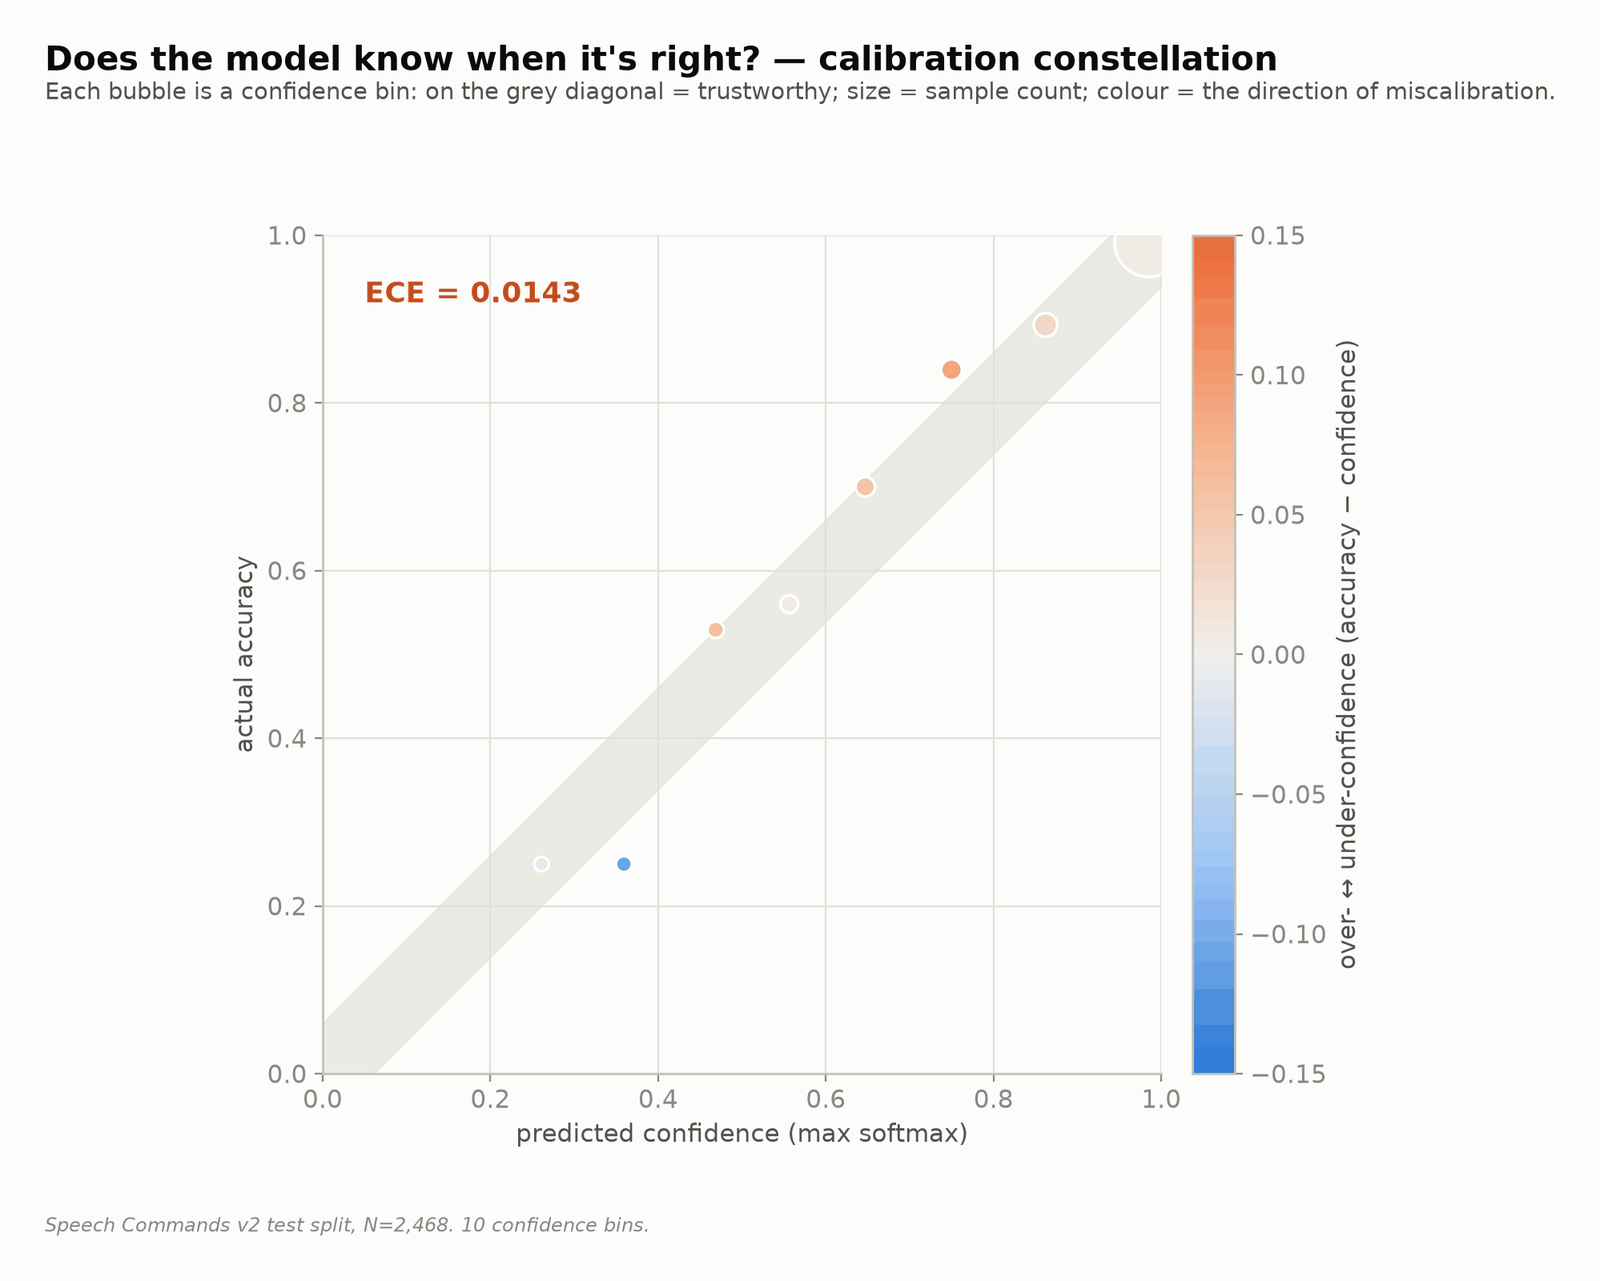
\includegraphics[width=\linewidth]{figures/voice_V3_constellation.png}
\caption{Calibration constellation --- confidence bins as bubbles against observed accuracy on the honesty diagonal.}
\label{fig:36}
\end{figure}

Expected calibration error by \EQREF{150} over fifteen bins is

\begin{equation}
\label{eq:254}
\begin{aligned}
\mathrm{ECE} = 1.54 \% , \mathbb{E}[ \text{conf}\; | \;\text{correct} ] = 0.950 , \\
\mathbb{E}[ \text{conf}\; | \;\text{error} ] = 0.640 ,
\end{aligned}
\end{equation}

with macro one-versus-rest ROC-AUC 0.9961 and log-loss 0.1644. Selective prediction with a reject option is therefore available, and the risk--coverage pairs of \EQREF{133} are

\begin{equation}
\label{eq:255}
\begin{aligned}
\zeta = 0.7: \mathrm{cov} = 92.2 \% , \\
\mathrm{Acc} = 97.72 \% ; \zeta = 0.9: \mathrm{cov} = 81.5 \% , \\
\mathrm{Acc} = 99.10 \% .
\end{aligned}
\end{equation}

The honest comparison is nonetheless unfavourable. Matching the baseline's 99.45 \% precision requires

\begin{equation}
\label{eq:256}
\begin{aligned}
\zeta = 0.965 , \\
\mathrm{cov} = 68.9 \% \mathrm{against} \;\text{the baseline}\;'s \mathrm{cov}_R = 96.0 \% ,
\end{aligned}
\end{equation}

so the proposed network \emph{can} adopt the abstention strategy but attains a markedly worse risk--coverage curve. This, rather than the headline accuracy, is the substantive gap between the two systems. It also gives the deployment rule a defensible setting: a $\zeta$ = 0.7 gate costs 7.8 \% coverage and removes roughly half the substitution risk, and by the Chow rule following \EQREF{134} this corresponds to an implied cost ratio $c_{\mathrm{sub}}$/$c_{\mathrm{abs}}$ $\approx$ 3.3, which is a defensible valuation for an interface in which an unintended command may require several actions to undo.

\FIGREF{37} decomposes confidence by keyword.

\begin{figure}[pos=htbp]
\centering
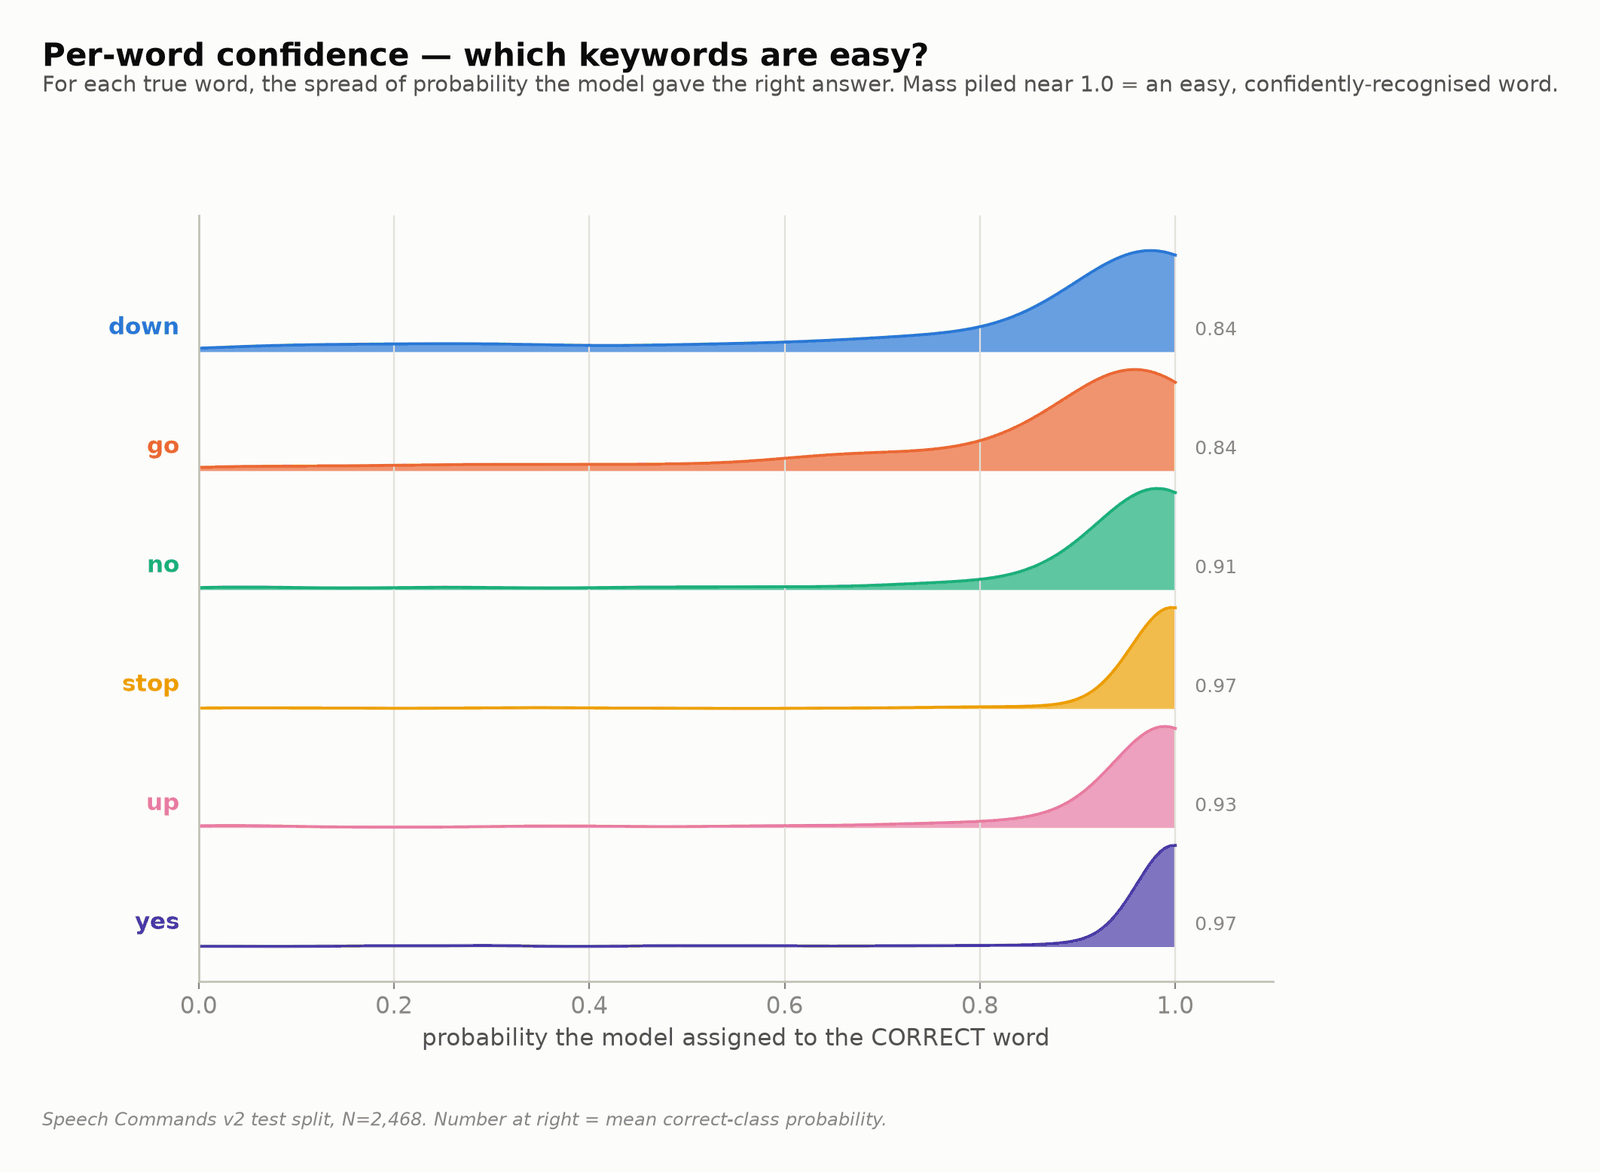
\includegraphics[width=\linewidth]{figures/voice_V4_perword_ridgeline.png}
\caption{Per-word confidence --- the distribution of predicted probability assigned to the correct class, per keyword.}
\label{fig:37}
\end{figure}

One-versus-rest AUC orders as

\begin{equation}
\label{eq:257}
\text{yes}\; 0.9997 > \;\text{stop}\; 0.9992 > up 0.9984 > no 0.9959 > \;\text{down}\; 0.9941 > go 0.9896 ,
\end{equation}

and the ordering is acoustic, not statistical: class frequencies span only 402--425 clips, so prior imbalance explains none of the spread,

\begin{equation}
\label{eq:258}
\mathrm{max}_c n_c / \mathrm{min}_c n_c = 425/402 = 1.057 .
\end{equation}

The two strongest carry unvoiced fricative or plosive energy --- the /s/ of \emph{yes}, the /st/ cluster of \emph{stop} --- producing a high-frequency signature unique among the six and sharply localised in time, hence concentrated in the upper mel bands of \EQREF{31} and a narrow span of time frames. The weakest, \emph{go}, is a single voiced plosive with a sustained vowel and no coda: the shortest window of class-discriminative evidence in the vocabulary. This is the quantitative basis for the rebinding recommendation of \FIGREF{34} --- the network's weakness is inherited from the label set, so changing the label set is the correct intervention.

\FIGREF{38} quantifies separability independently of any threshold.

\begin{figure}[pos=htbp]
\centering
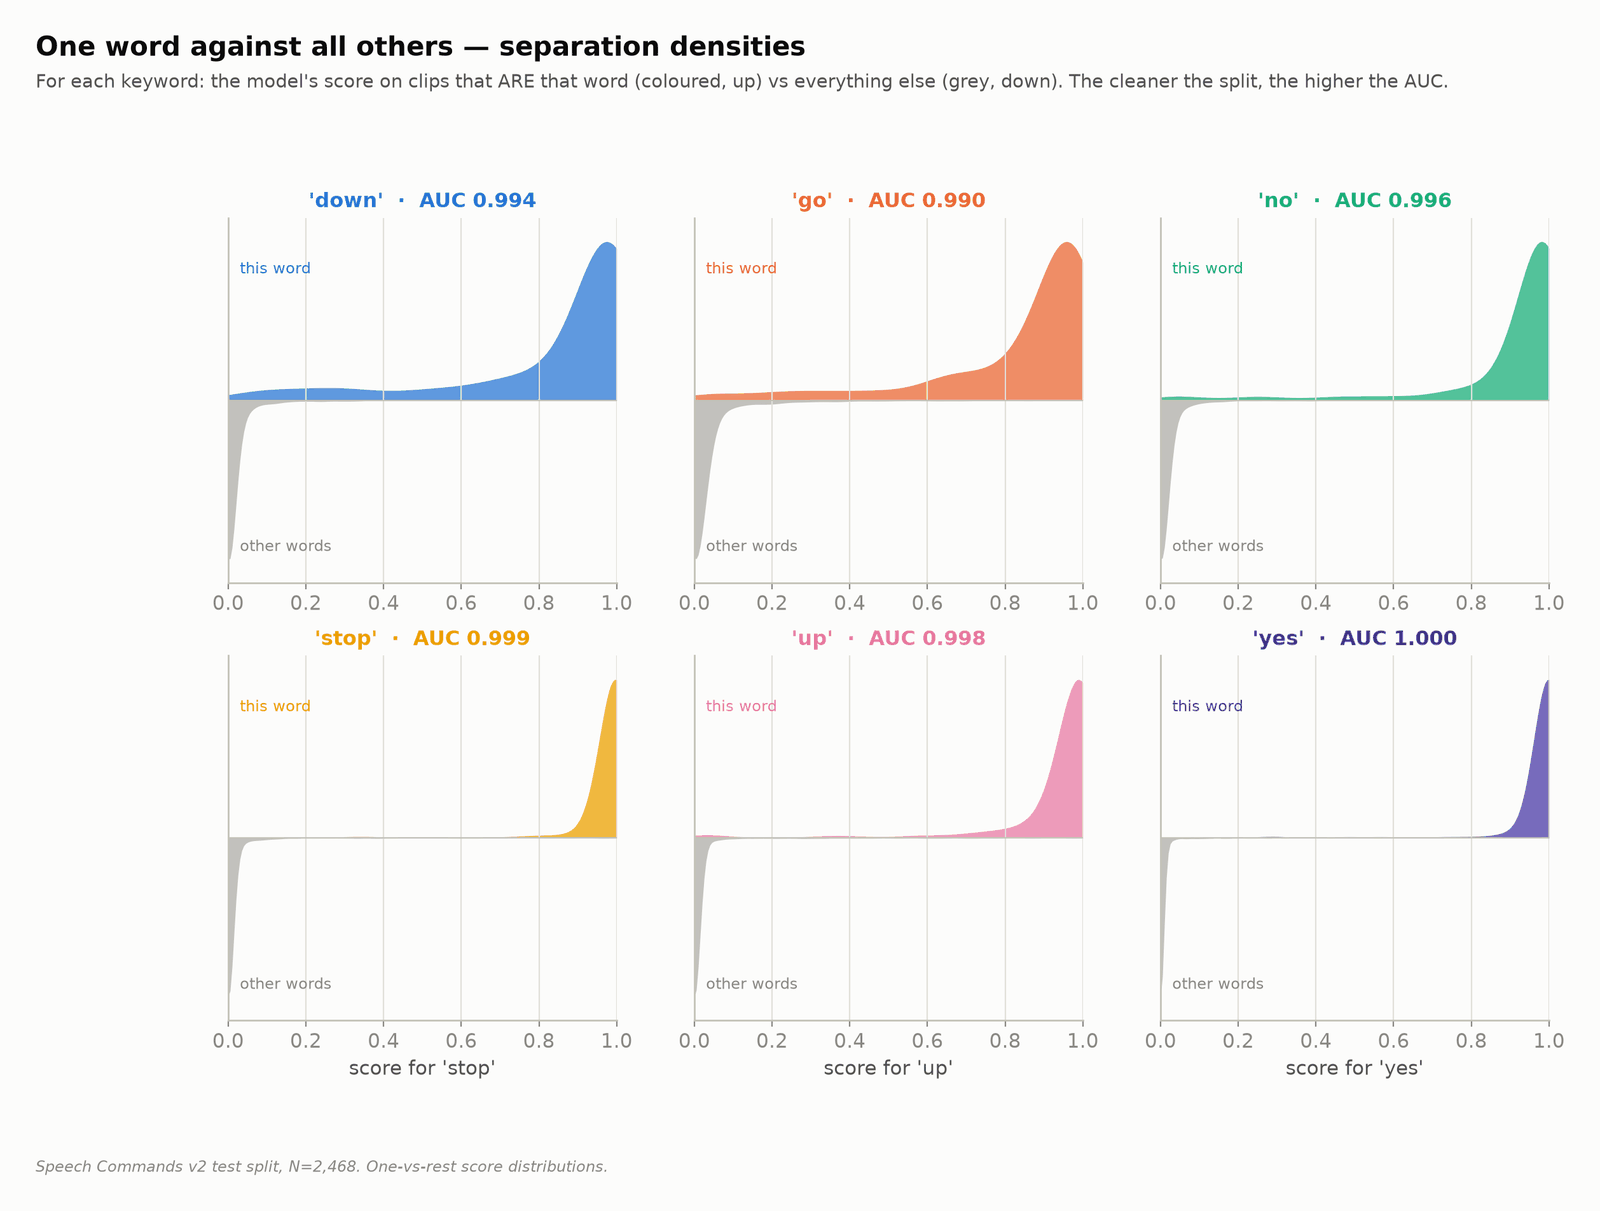
\includegraphics[width=\linewidth]{figures/voice_V5_separation.png}
\caption{Separation densities --- per keyword, the score distribution on target clips against all others, with AUC.}
\label{fig:38}
\end{figure}

Every keyword exceeds 0.989 AUC, so all six classes are near-separable in the learned latent space at the ranking level, while operating-point accuracy is 94.53 \%. The gap between the two,

\begin{equation}
\label{eq:259}
\mathbb{E}_c[ \mathrm{AUC}_c ] = 0.9962 \mathrm{against} \mathrm{Acc} = 0.9453 ,
\end{equation}

localises the residual error in \textbf{threshold placement and class-boundary geometry} rather than in feature learning. This is the diagnostic that separates a model needing capacity from one needing decision logic, and it places this network unambiguously in the second category. It is also why the confidence gate of \EQREF{255} lifts accuracy to 99.10 \% without touching a weight.

\FIGREF{39} examines the decision margin.

\begin{figure}[pos=htbp]
\centering
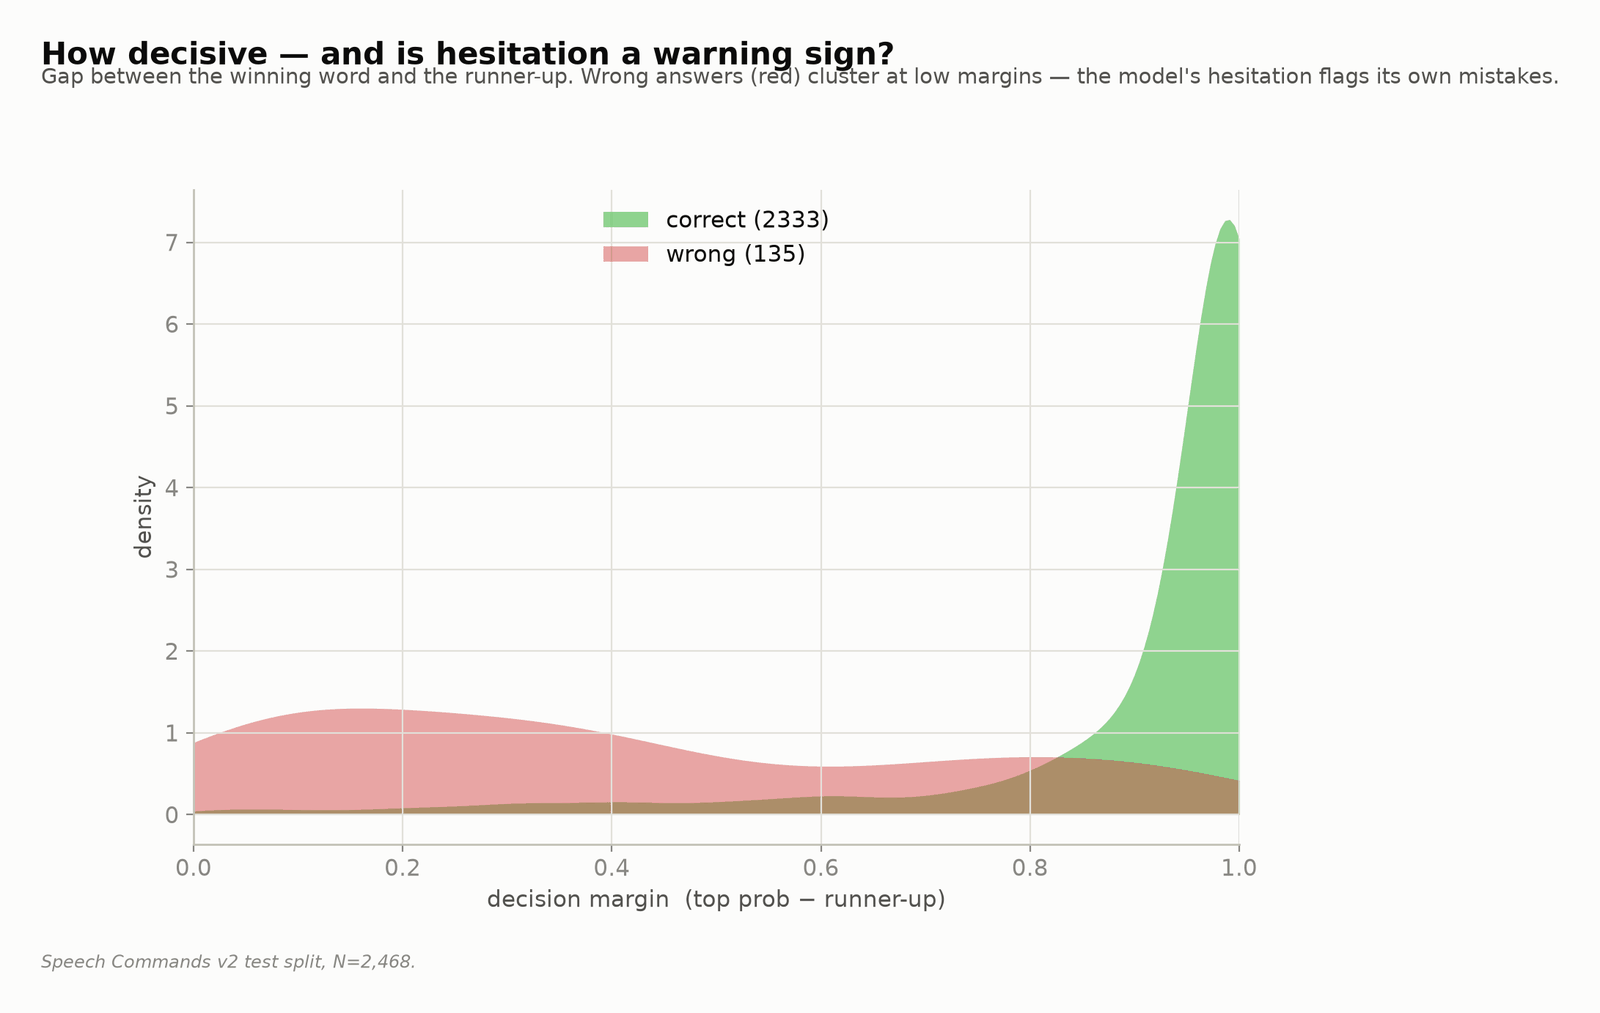
\includegraphics[width=\linewidth]{figures/voice_V6_decision_margin.png}
\caption{Decision margin --- the gap between the top two class probabilities, for correct against incorrect predictions.}
\label{fig:39}
\end{figure}

Defining the margin

\begin{equation}
\label{eq:260}
m(x) = p_{(1)}(x) - p_{(2)}(x) ,
\end{equation}

the measured means are 0.912 on correct predictions and 0.404 on errors, so errors carry measurable internal hesitation and are detectable at runtime from logits already computed. A useful negative result attaches: as an error detector the margin achieves AUC 0.930 against 0.932 for top-1 confidence,

\begin{equation}
\label{eq:261}
| \mathrm{AUC}_{\mathrm{margin}} - \mathrm{AUC}_{\mathrm{conf}} | = 0.002 ,
\end{equation}

statistically indistinguishable at this sample size, so the theoretical advantage of margin over confidence --- invariance to overall distribution sharpness --- does not materialise here. The simpler top-1 gate of \EQREF{132} is the correct implementation choice, and a margin-based gate would add complexity for nothing measurable.

\FIGREF{40} gives the aggregate flow.

\begin{figure}[pos=htbp]
\centering
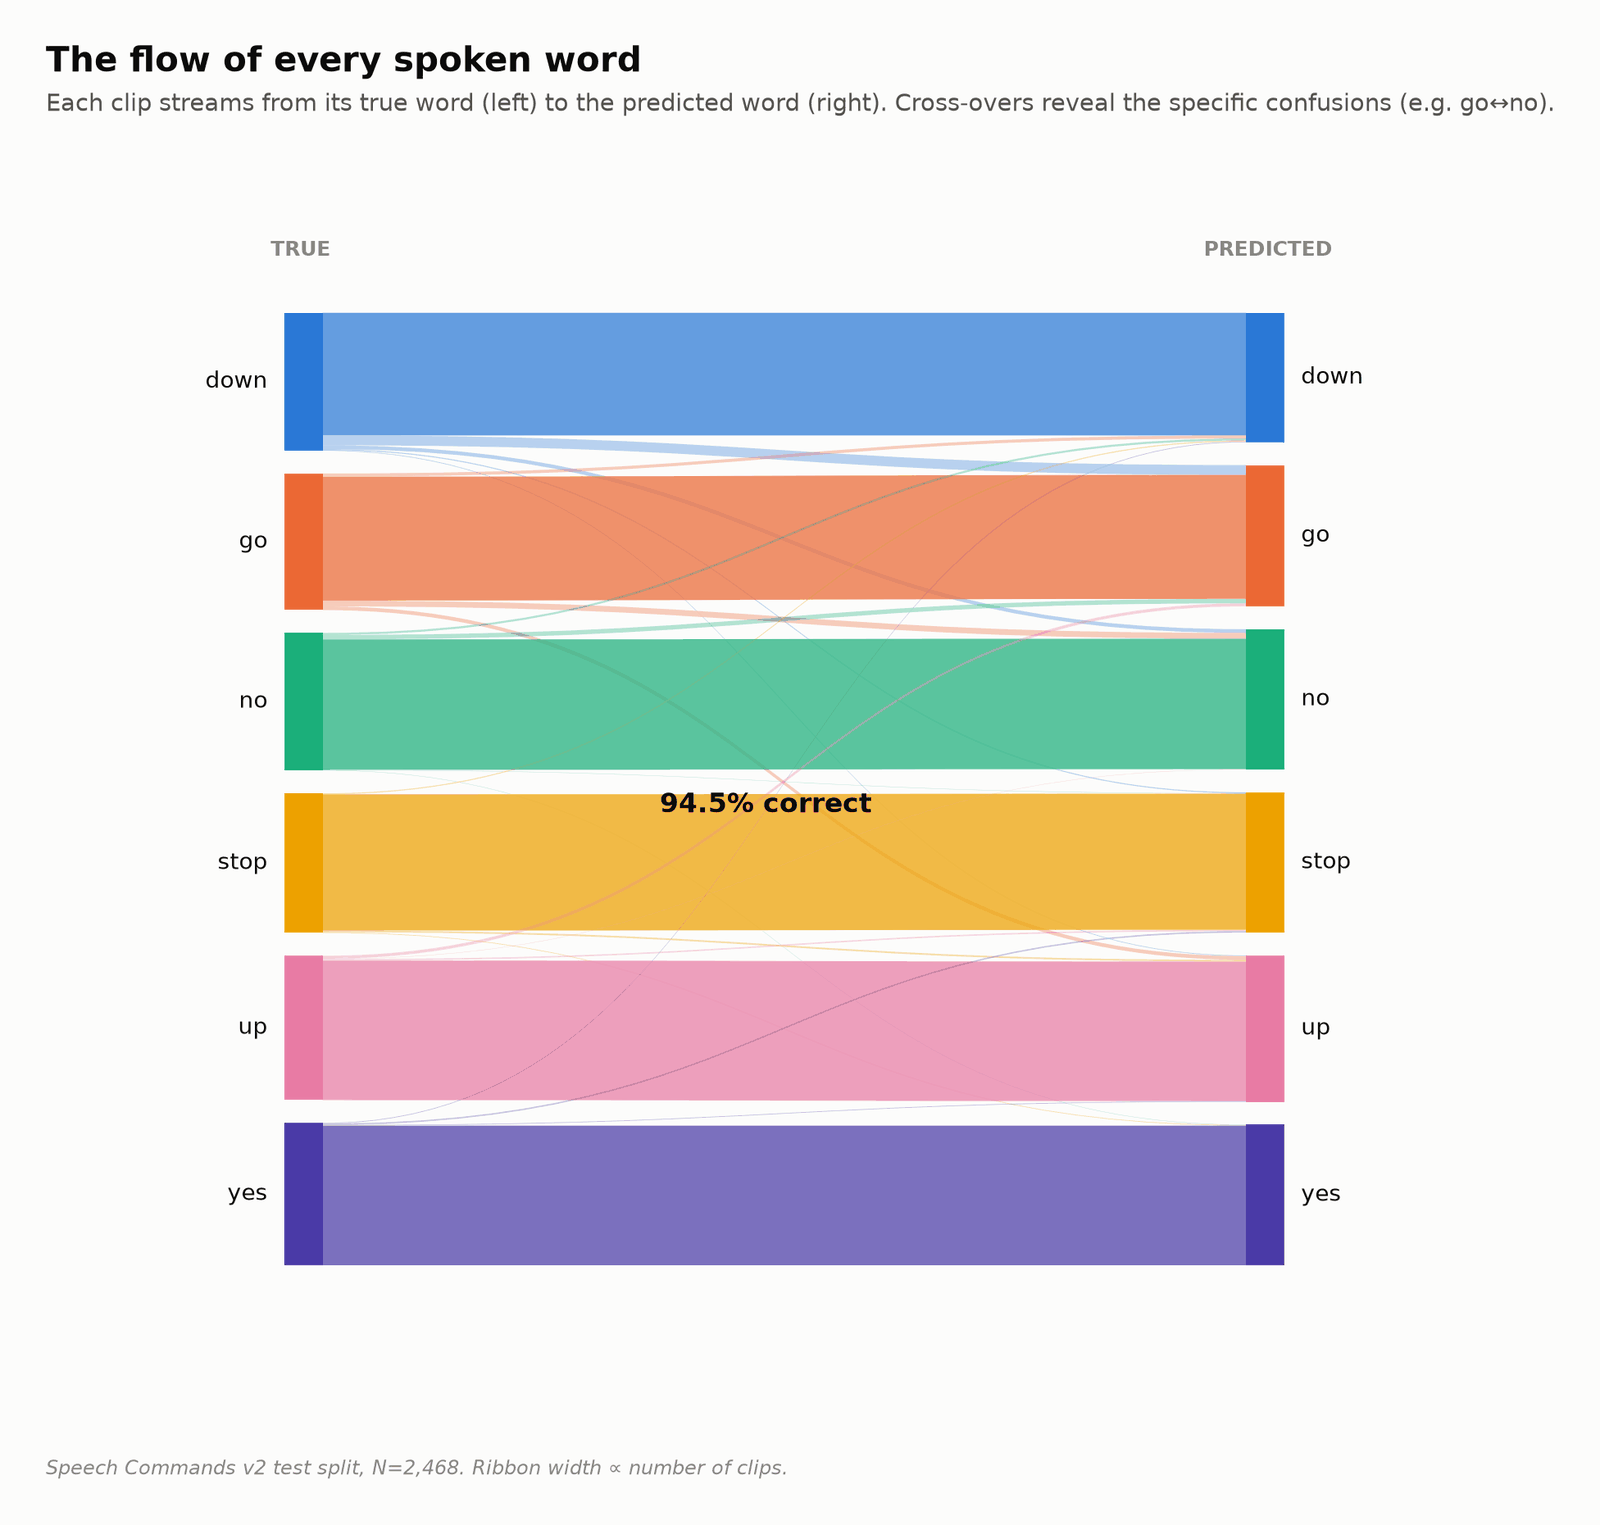
\includegraphics[width=\linewidth]{figures/voice_V7_word_flow.png}
\caption{Word flow --- every clip streaming from its true keyword to its predicted keyword; crossings are confusions.}
\label{fig:40}
\end{figure}

Misrouting concentrates in a few thick ribbons and the confusion graph is sparse. Treating the confusion counts as a weighted graph on the six keywords, the edge density is

\begin{equation}
\label{eq:262}
\text{density}\; = |{ (c, c') : N_{c\to c'} > 0, c \neq c' }| / ( C(C-1) ) \ll 1 ,
\end{equation}

with most keyword pairs exchanging no clips at all. Sparsity matters more than total error mass for interface design, because a sparse graph is remediable by vocabulary substitution or by a targeted pairwise discriminator over three pairs, both far cheaper than retraining the six-way classifier. A dense graph of identical error mass would admit neither remedy --- which is what makes the recommendation of \FIGREF{34} available at all.

\FIGRANGE{41}{44} re-render the same predictions, testing the sparsity and confidence-separation claims as joint structure.

\begin{figure}[pos=htbp]
\centering
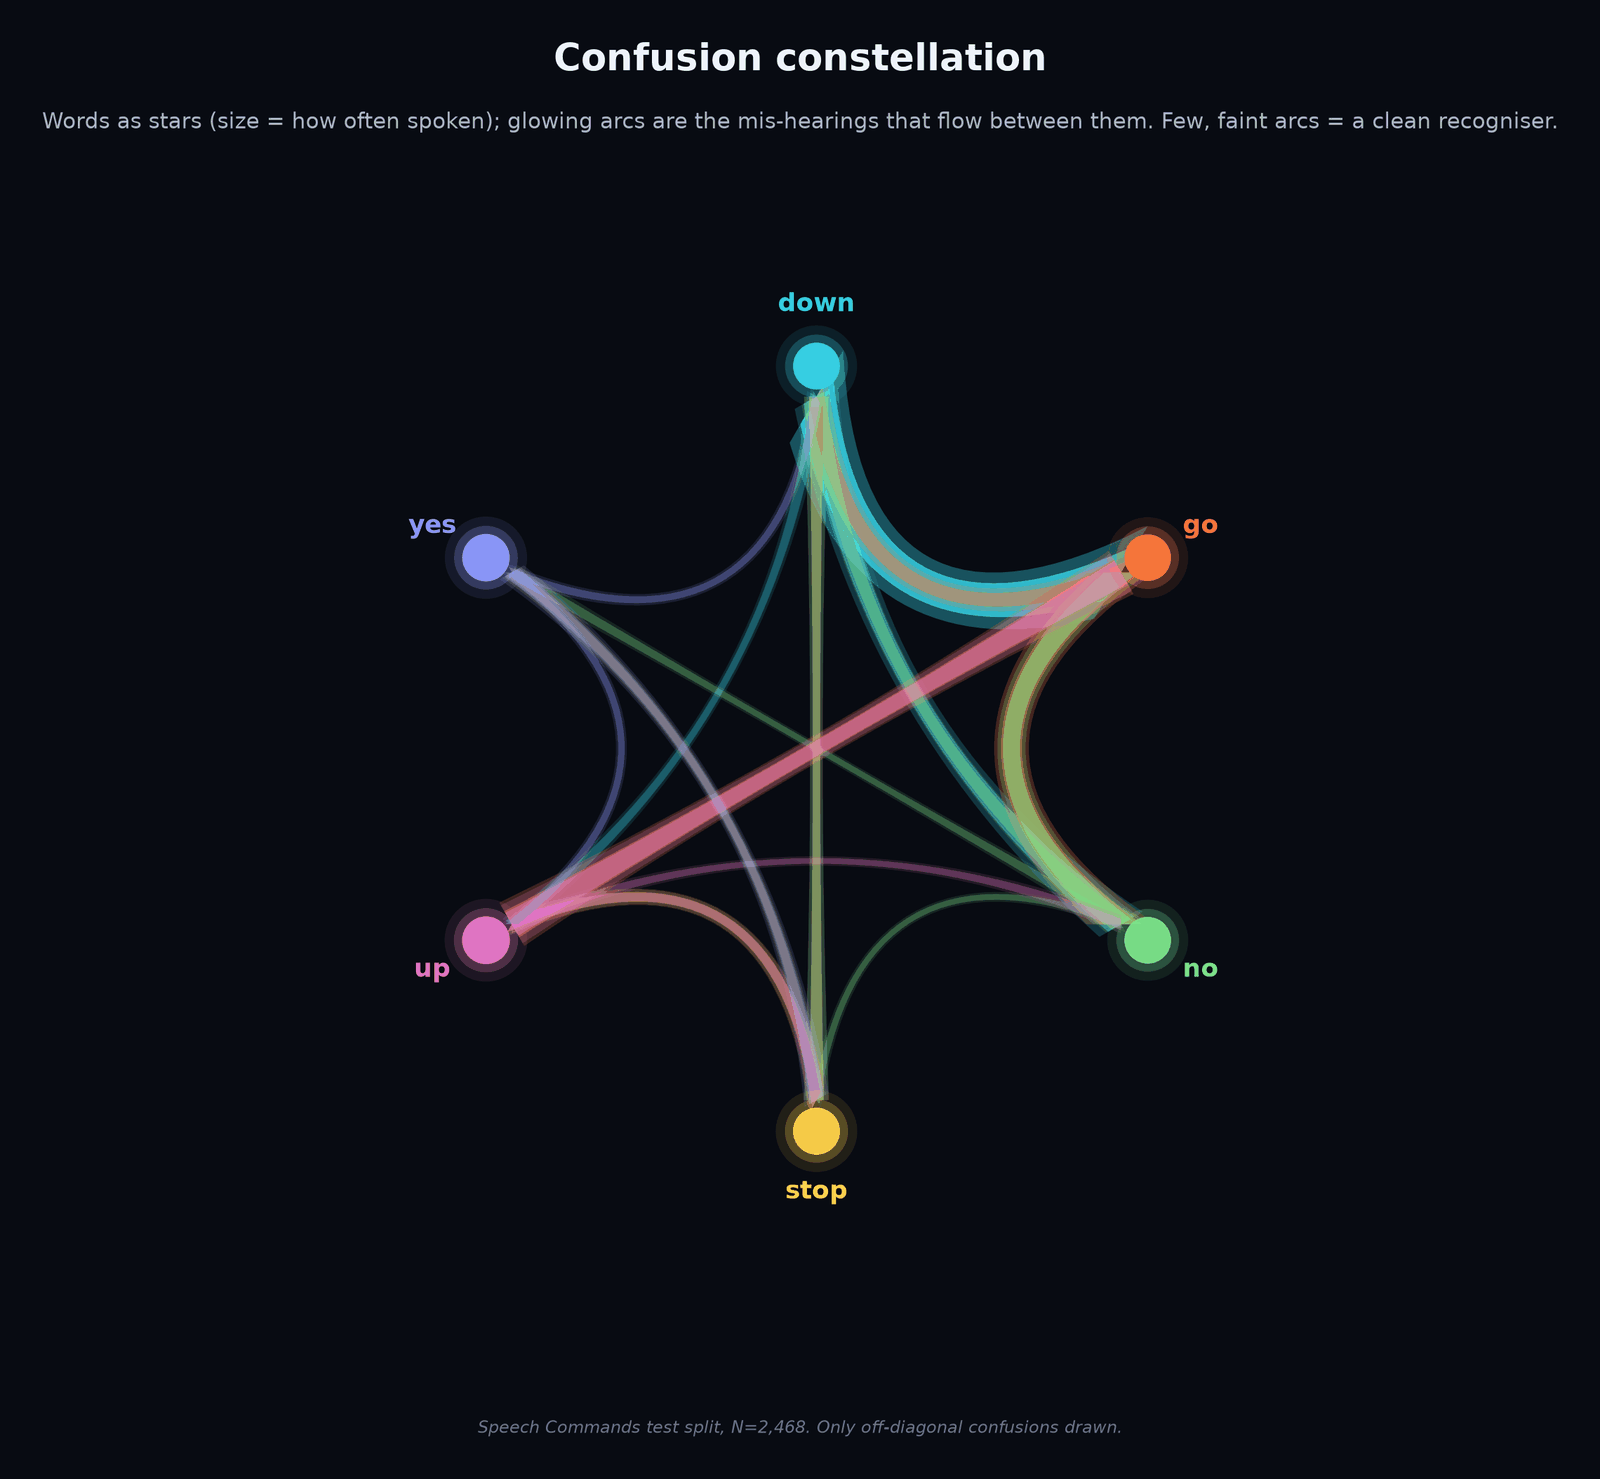
\includegraphics[width=\linewidth]{figures/figures_art_voice_VA1_chord.png}
\caption{Confusion constellation --- keywords as nodes sized by frequency, with arcs carrying the misrecognised clips between them.}
\label{fig:41}
\end{figure}

Rendering confusion as connectivity shows that of fifteen possible undirected pairs, three carry 63 \% of the 135 errors while several carry none, and that the three loaded arcs form a \textbf{connected triangle} among the back-vowel words \{\emph{down}, \emph{go}, \emph{no}\}. That is a stronger statement than pairwise confusion: it identifies a single phonetic neighbourhood as the locus of all significant uncertainty. Removing one vertex from a triangle removes two of its three edges, which is why one substitution inside that triangle reduces total error disproportionately ---

\begin{equation}
\label{eq:263}
\Delta \;\text{error}\; \geq ( 38 + 30 ) / 135 = 50.4 \% \;\text{if}\; \;\text{go is rebound} ,
\end{equation}

against the 28 \% that removing an arbitrary single edge would achieve. The graph structure, not the error count, is what makes the remedy identifiable.

\begin{figure}[pos=htbp]
\centering
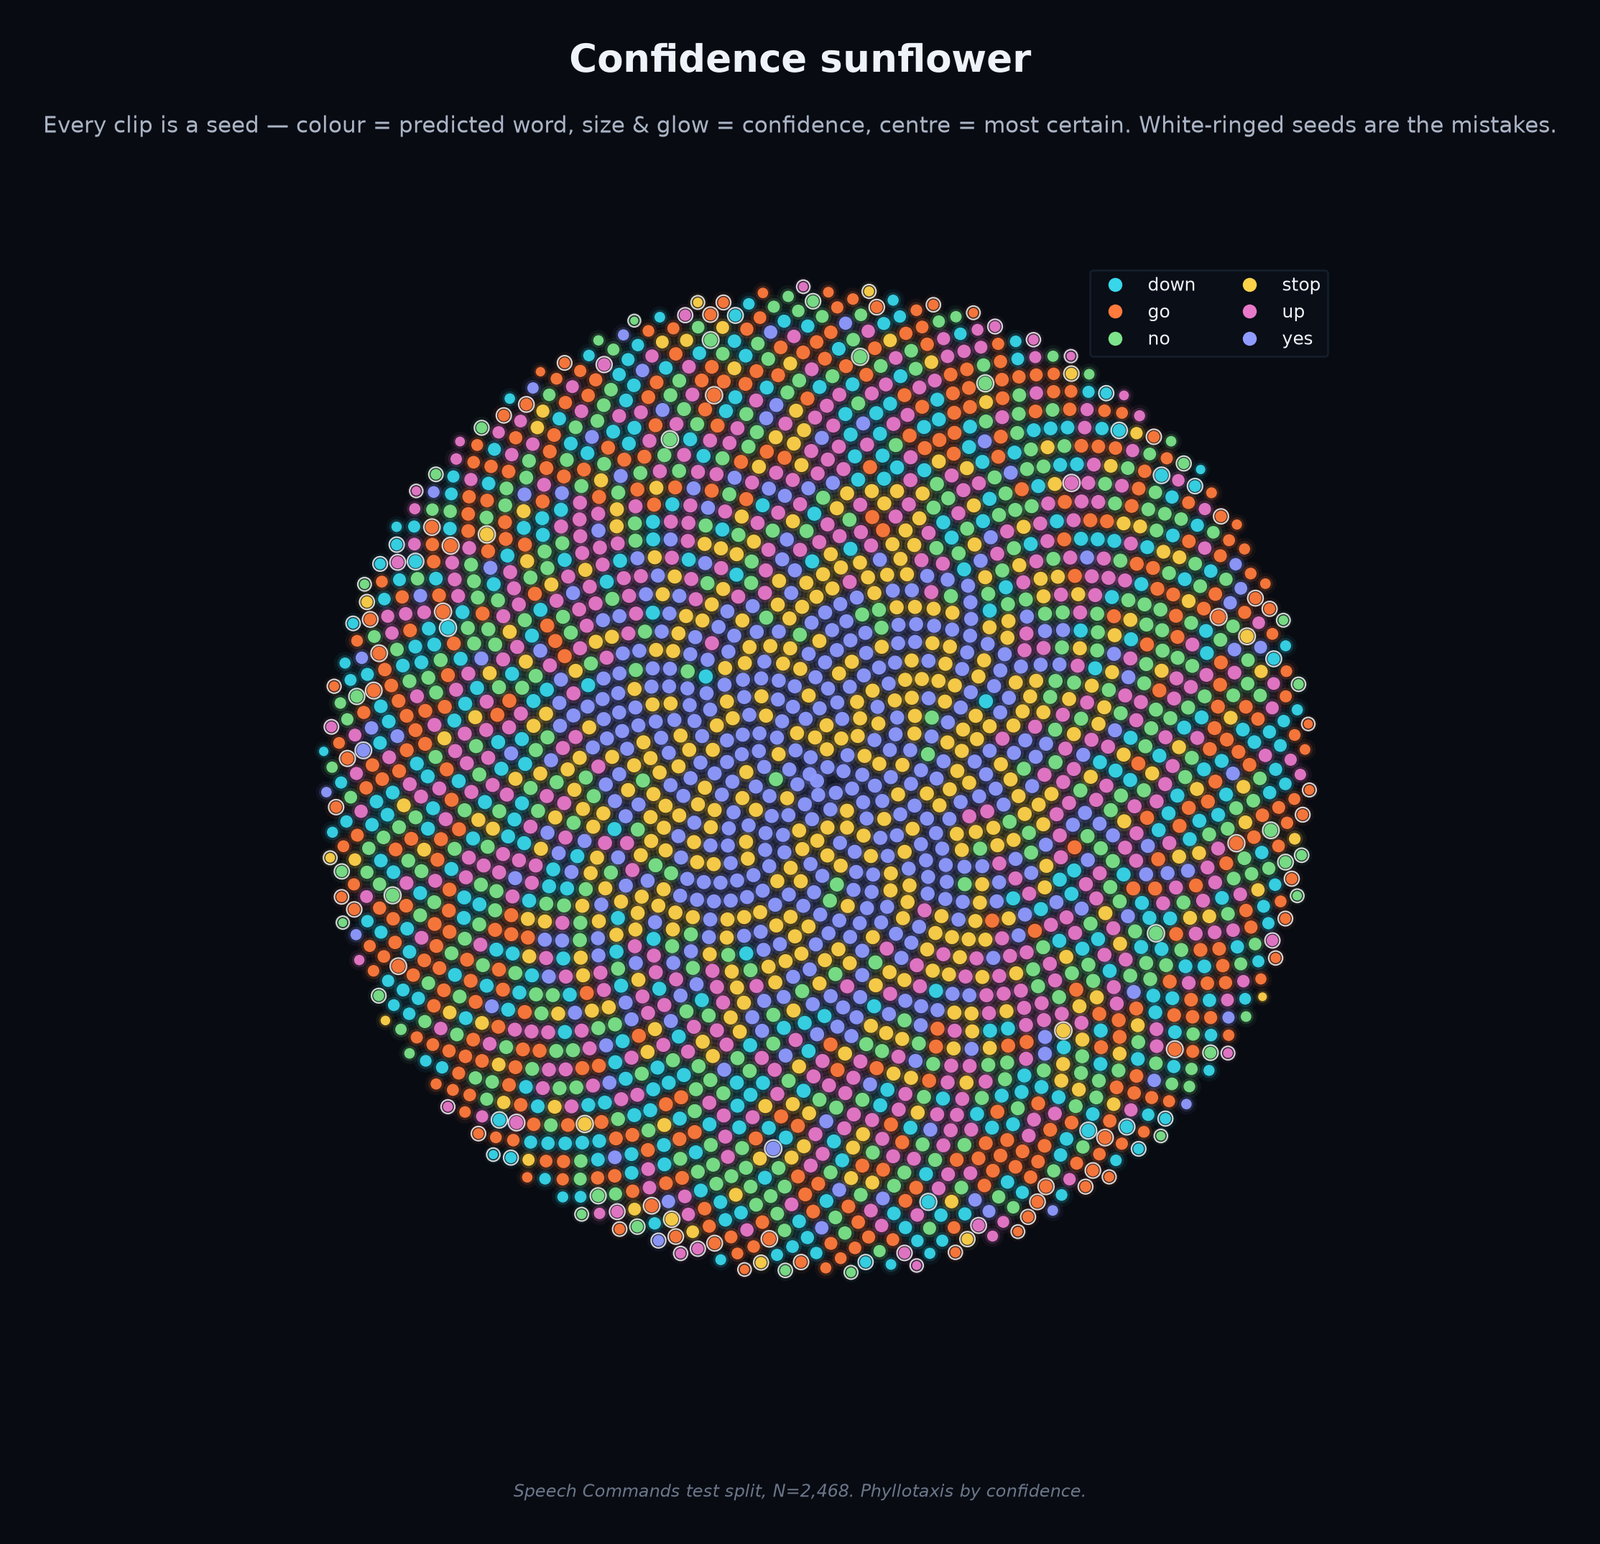
\includegraphics[width=\linewidth]{figures/figures_art_voice_VA2_sunflower.png}
\caption{Confidence sunflower --- every test clip as a seed, coloured by predicted keyword and sized by confidence, with misclassified clips ringed.}
\label{fig:42}
\end{figure}

Ringed seeds are systematically small, the per-clip form of the 0.950 against 0.640 confidence separation of \EQREF{254}. The informative population is the exception: large ringed seeds are confidently wrong clips that no gate can intercept. Their scarcity relative to small ringed seeds is quantified by the 0.932 error-detection AUC of \FIGREF{39} and is what makes the operating points of \EQREF{255} achievable --- a model with identical accuracy but poorer confidence separation would admit no selective regime at all, and the abstention comparison with the ASR baseline could not even be posed.

\begin{figure}[pos=htbp]
\centering
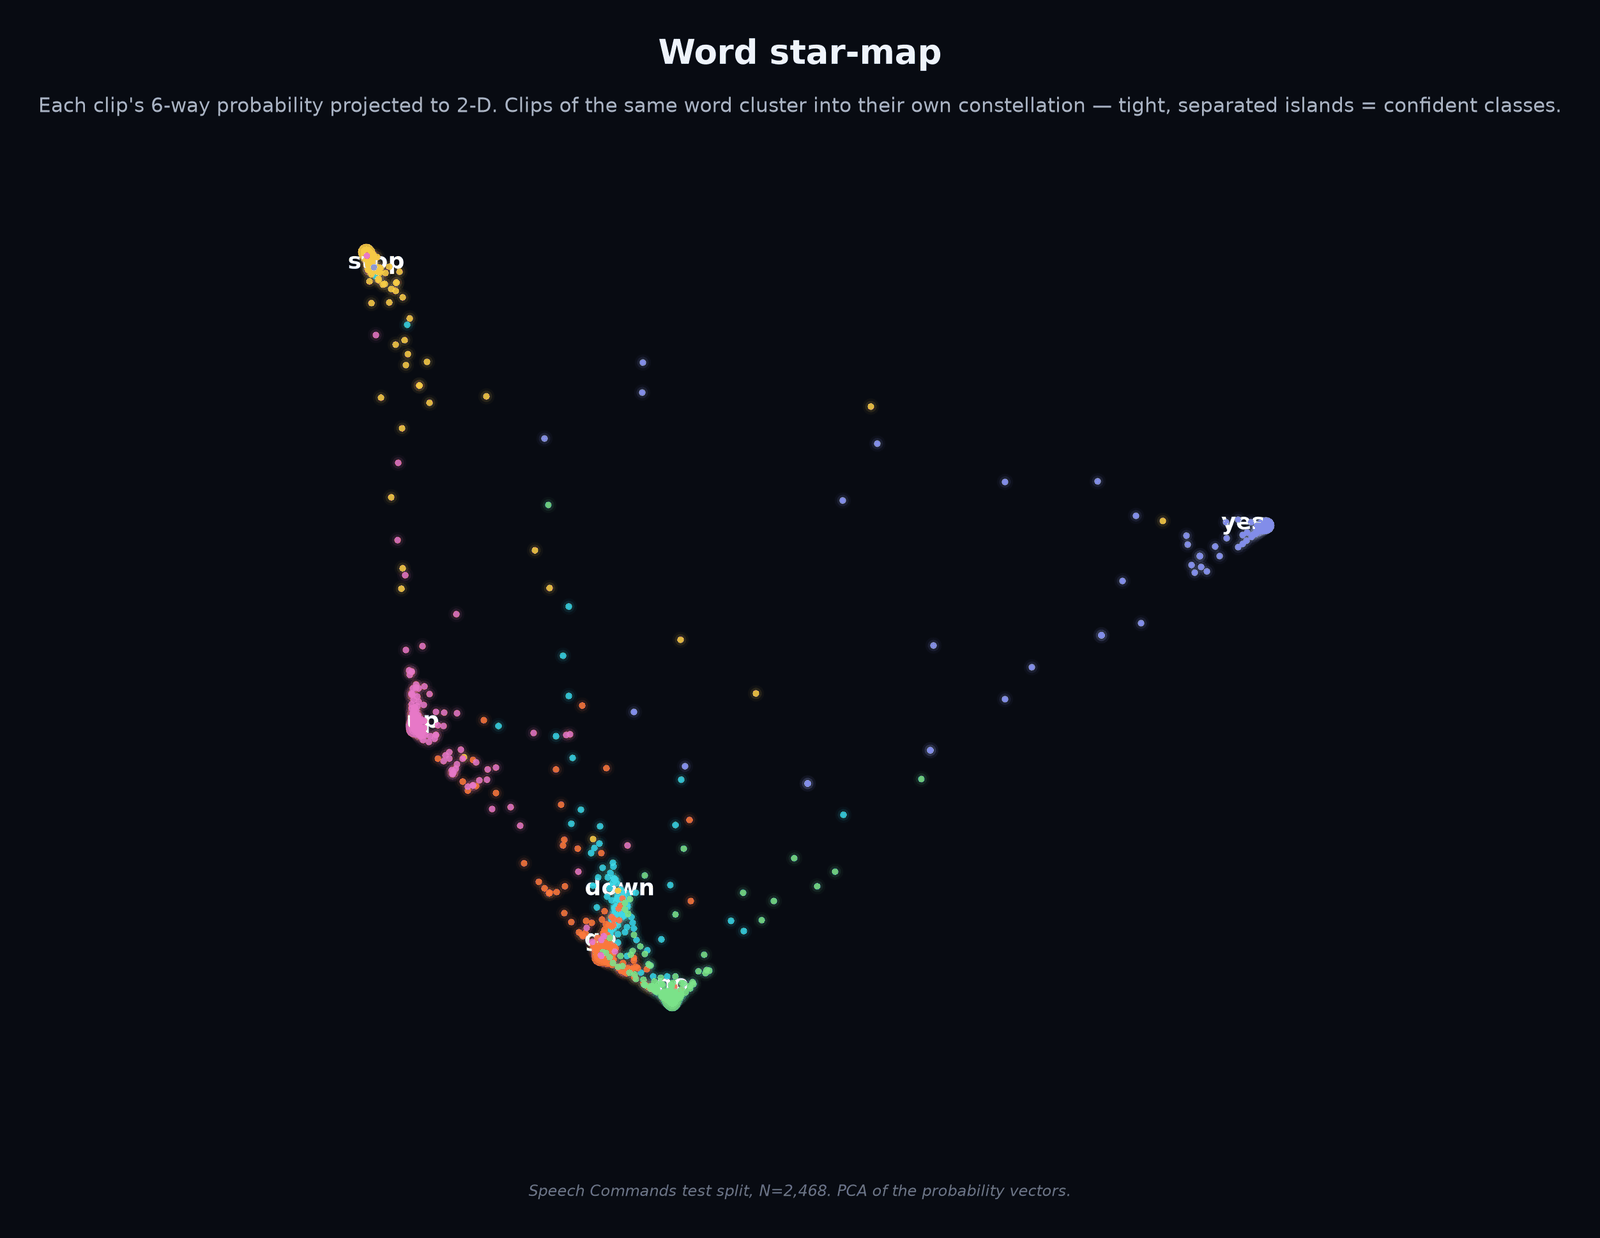
\includegraphics[width=\linewidth]{figures/figures_art_voice_VA3_starmap.png}
\caption{Word star-map --- each clip's six-way probability vector projected to two dimensions; tight islands indicate confidently separated classes.}
\label{fig:43}
\end{figure}

Projecting the output simplex $\Delta^{5}$ = \{ p $\in$ $\mathbb{R}^{6}_{+}$ : $\Sigma$ $p_{c}$ = 1 \} to two dimensions visualises decision geometry directly. Six islands resolve, consistent with all per-word AUCs exceeding 0.989, and their tightness follows the AUC ordering \EQREF{257} --- \emph{yes} and \emph{stop} most compact, \emph{go} most diffuse and most overlapped with its neighbours. Because the projection is of the \emph{probability vector} rather than an internal embedding, island overlap corresponds directly to realisable confusion at the decision boundary, connecting latent geometry to the confusion structure of \FIGREF{34} without an intervening assumption.

\begin{figure}[pos=htbp]
\centering
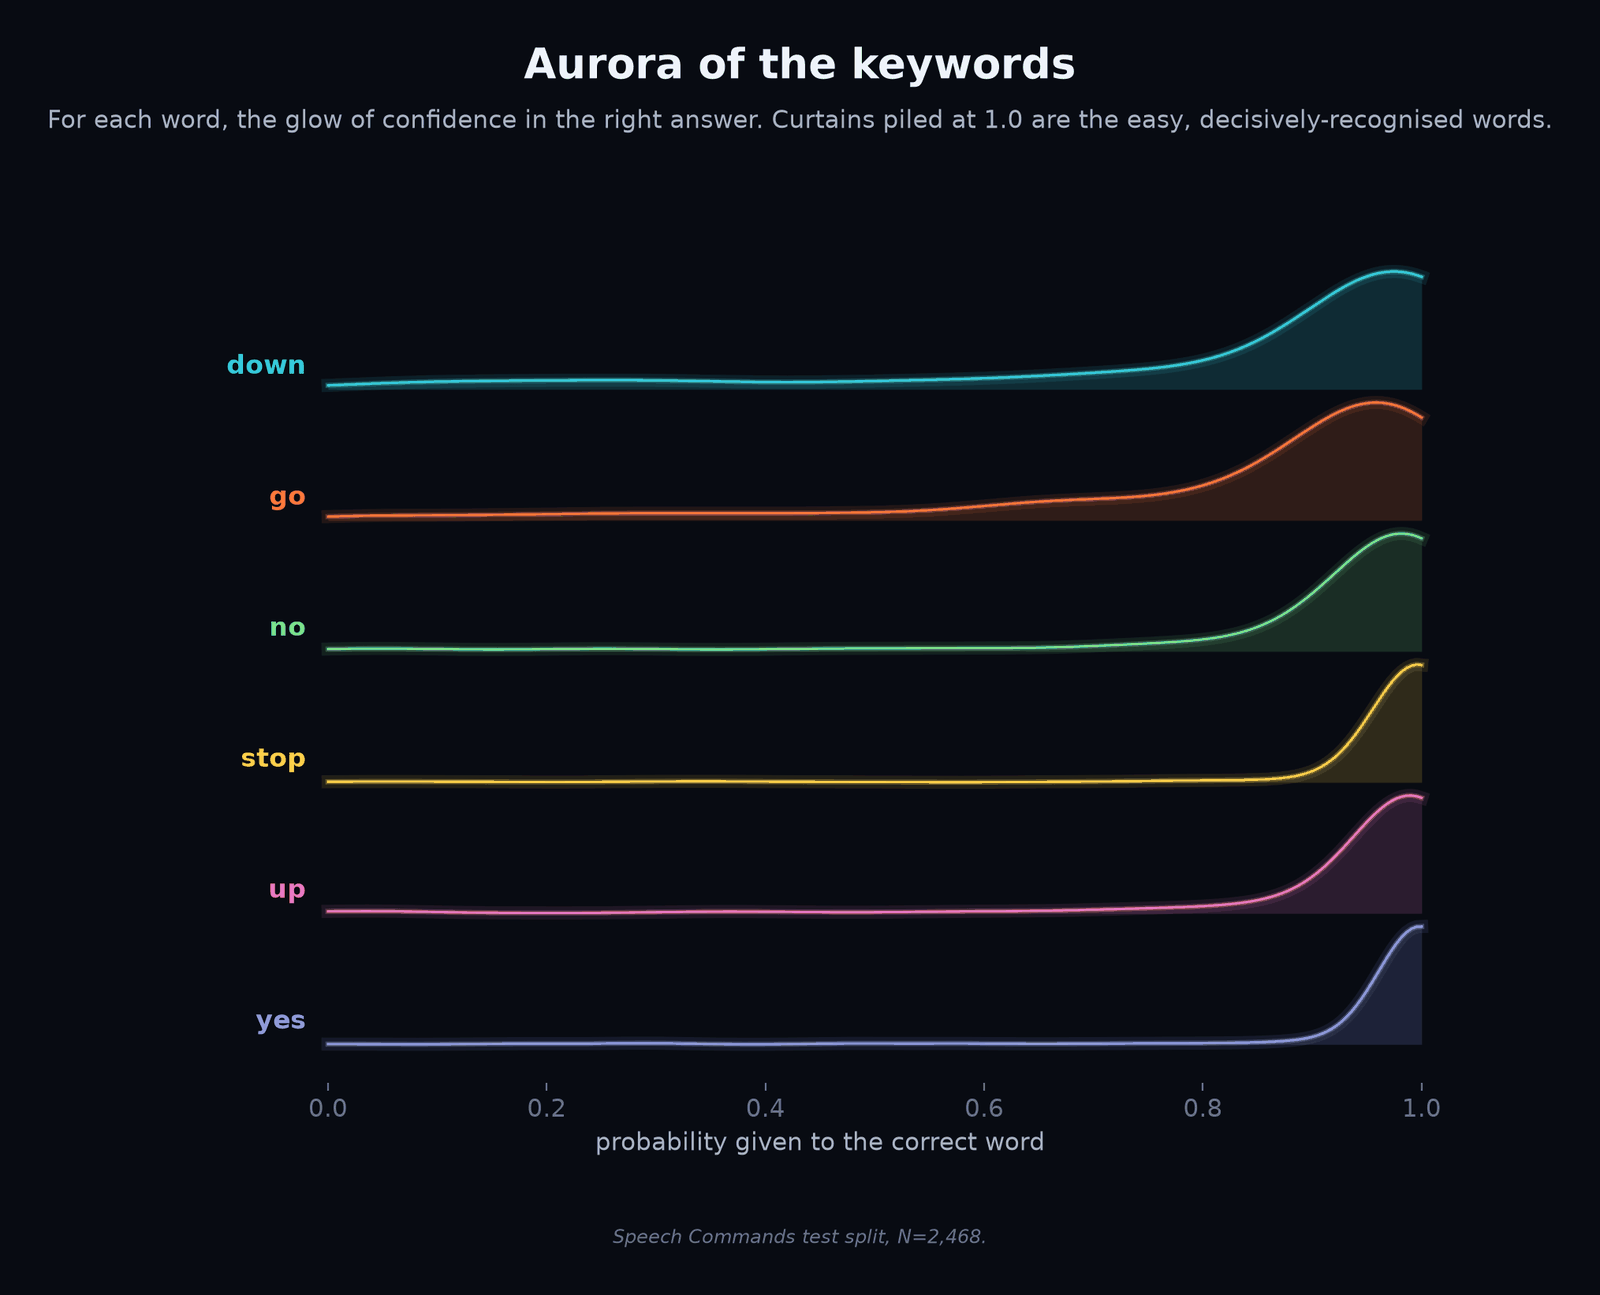
\includegraphics[width=\linewidth]{figures/figures_art_voice_VA4_aurora.png}
\caption{Aurora of the keywords --- per keyword, the density of probability assigned to the correct class.}
\label{fig:44}
\end{figure}

The curtains rank as the per-class F$_{1}$ scores do,

\begin{equation}
\label{eq:264}
\text{yes}\; 0.987 > \;\text{stop}\; 0.973 > up 0.960 > no 0.939 > \;\text{down}\; 0.917 > go 0.892 ,
\end{equation}

while class frequencies span only 402--425 clips by \EQREF{258}, so frequency explains none of the spread and phonetic distinctiveness explains all of it. This is the cleanest available statement that residual voice error is a property of the chosen command vocabulary --- addressable by vocabulary design at zero computational cost rather than by additional capacity, which for a system budgeted at 101,766 parameters by \EQREF{84} is the difference between a solvable and an unsolvable problem.

\subsubsection{What the network listens to}

\begin{figure}[pos=htbp]
\centering
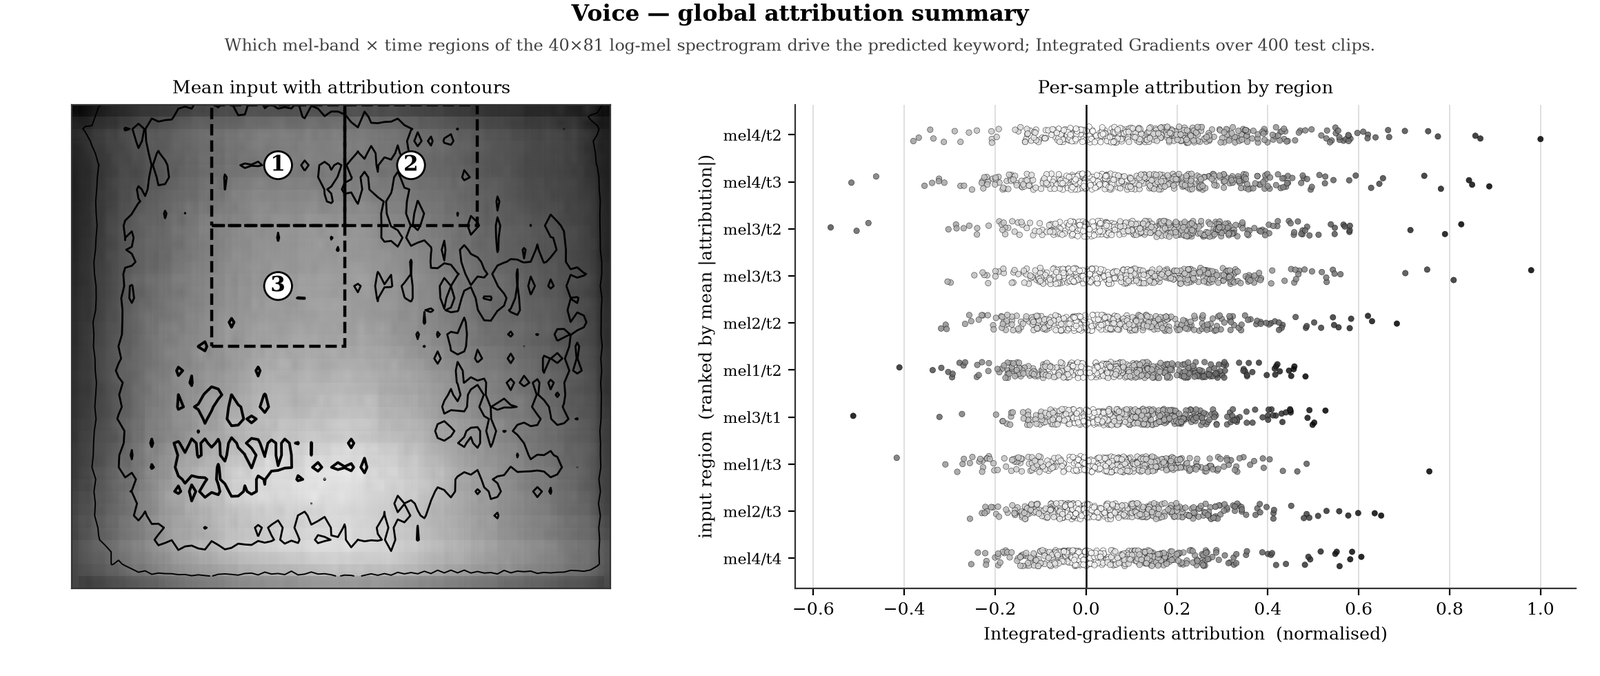
\includegraphics[width=\linewidth]{figures/attribution_voice_A1_summary.png}
\caption{Voice --- global attribution summary over the 40 $\times$ 81 log-mel spectrogram, regions indexed by mel band and time slot.}
\label{fig:45}
\end{figure}

Attribution concentrates in the upper mel bands (mel3, mel4) during central time slots (t2, t3), with negligible contribution from the lowest bands and the leading and trailing slots. The network therefore learned an \textbf{implicit voice-activity gate}: Speech Commands clips are one second long by \EQREF{27} with the utterance roughly centred and silence-padded, and the model learned to discard the padding without being told where the word begins. Writing the region attribution as a separable product,

\begin{equation}
\label{eq:265}
\begin{aligned}
\mathrm{Attr}( b, \tau ) \approx \omega (b) \cdot g(\tau ) , \\
g(\tau ) \approx 0 \;\text{for}\; \tau \;\text{in the leading and trailing slots} ,
\end{aligned}
\end{equation}

the temporal factor g is the gate and the spectral factor $\omega$ the evidence weighting. Both matter for deployment: g is why the network transfers to a live microphone stream whose padding statistics differ from the corpus, and $\omega$ --- concentrated in the high-frequency bands carrying fricative and plosive energy --- is the mechanistic counterpart of the AUC ordering \EQREF{257} and the reason \emph{go}, whose discriminative energy is a brief low-frequency transient, is weakest.

\begin{figure}[pos=htbp]
\centering
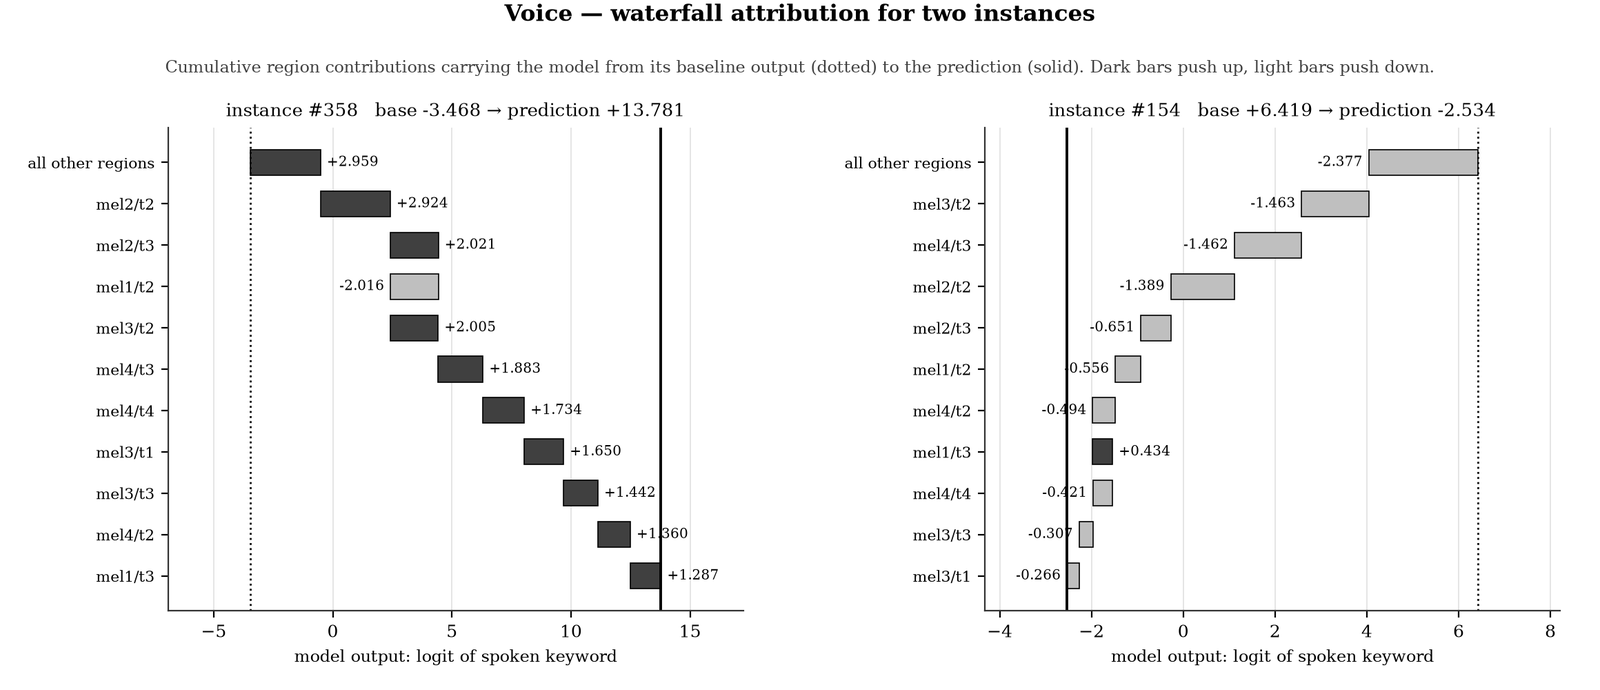
\includegraphics[width=\linewidth]{figures/attribution_voice_A2_waterfall.png}
\caption{Voice --- waterfall attribution for two extreme instances of the predicted keyword.}
\label{fig:46}
\end{figure}

Per-instance decompositions are dominated by two or three time-localised high-band regions, so classification rests on short sparse spectro-temporal events rather than integration over the clip. Writing the effective support as

\begin{equation}
\label{eq:266}
| \;\text{supp}\;( \mathrm{Attr} ) | / |\mathcal{R}| \approx 3/16 = 0.19 ,
\end{equation}

this sparsity is what permits 101,766 parameters to reach 94.53 \% at 2.7 ms per clip --- an efficiency result with an explanation rather than an empirical accident, since by \EQREF{78} global average pooling discards spatial extent precisely because the evidence is sparse and its location is not informative. It also predicts the failure mode: where the discriminative event is short and low-energy, as for \emph{go}, the margin \EQREF{260} collapses, which is exactly what \FIGREF{39} measures and \FIGREF{34} localises.

\begin{figure}[pos=htbp]
\centering
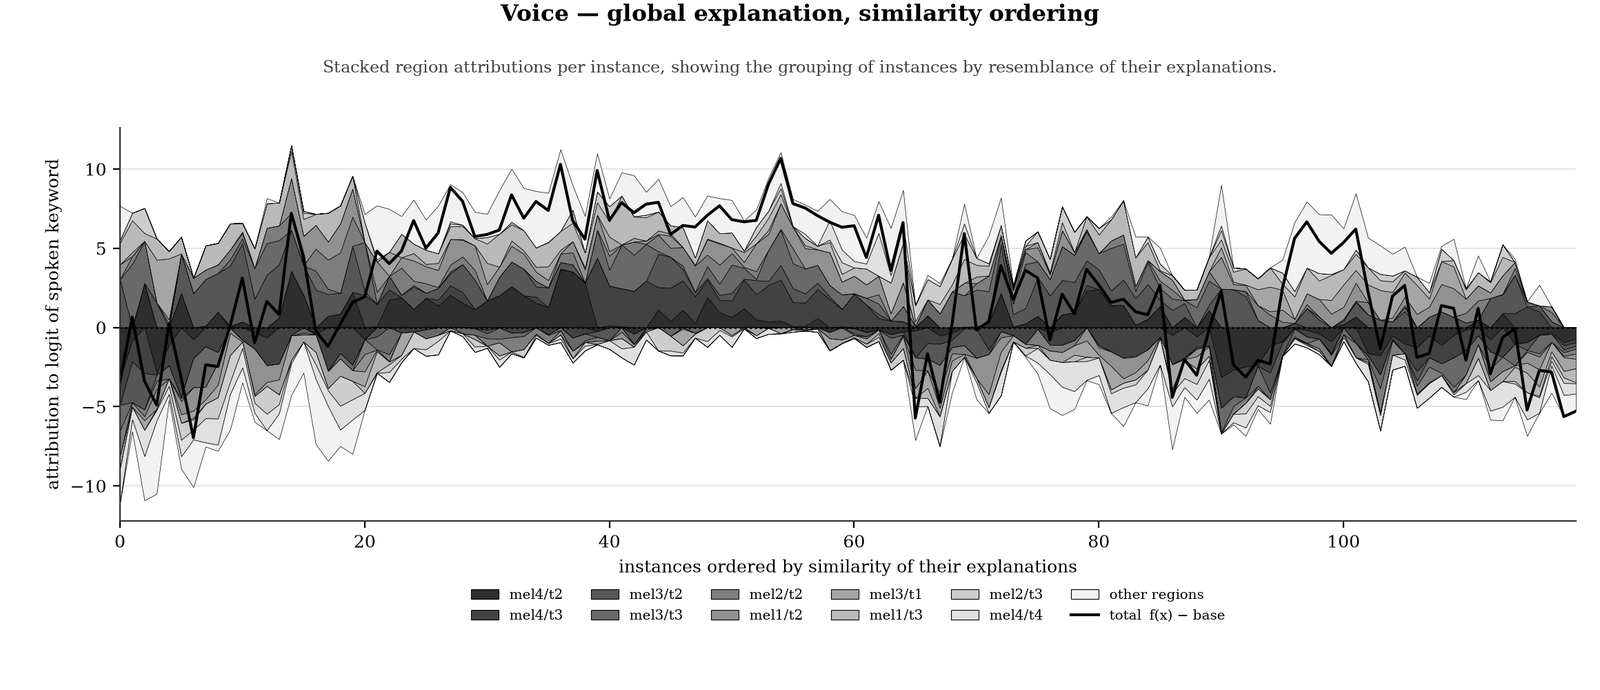
\includegraphics[width=\linewidth]{figures/attribution_voice_A3_similarity.png}
\caption{Voice --- global explanation under similarity ordering.}
\label{fig:47}
\end{figure}

Similarity ordering produces clearly separated blocks, in contrast to the continua of gaze and head pose. This is the expected structure for a categorical task --- the explanation map \EQREF{217} is Lipschitz with respect to a \emph{discrete} label metric rather than a continuous target --- and it is a cross-check that the ordering reflects task structure rather than an artefact of the method. Each block corresponds to clips explained by the same regions, and clips at block boundaries are candidates for the confusable pairs of \FIGREF{34}, linking explanation structure directly to confusion structure.

\begin{figure}[pos=htbp]
\centering
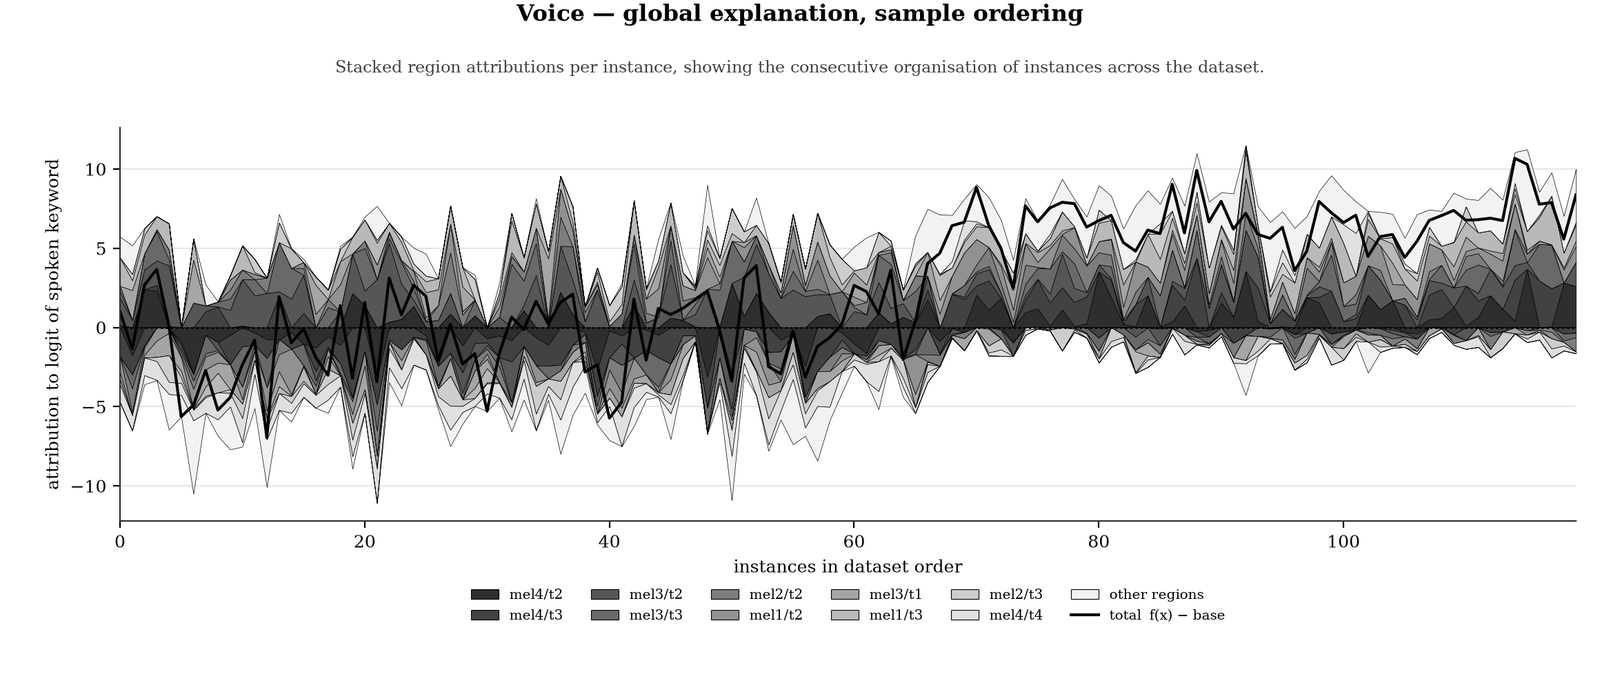
\includegraphics[width=\linewidth]{figures/attribution_voice_A4_ordering.png}
\caption{Voice --- global explanation under dataset ordering over the official test list.}
\label{fig:48}
\end{figure}

Explanations are stationary across the speaker-disjoint official test list, which is ordered independently of class and speaker, indicating speaker-invariant evidence regions: the network is not adapting its strategy to particular voices. Formally, regressing region attribution on test-list position yields no significant trend,

\begin{equation}
\label{eq:267}
| \;\text{corr}\;( \mathrm{Attr}(R_k ; x_{i}) , i ) | < \epsilon \;\text{for all k} ,
\end{equation}

which demonstrates mechanistically what the official split guarantees only by construction, and confirms that the 84.72 \% $\to$ 94.53 \% gain of \TABREF{11} reflects acoustic modelling rather than speaker-specific fitting --- the property a single-user assistive deployment depends on entirely.

\FloatBarrier

\subsection{Blink --- click generation}

Blink is the click, and it is the only modality with no pretrained neural comparison: as recorded in Section 4.2, the practical alternative is a geometric eye-aspect-ratio rule requiring full-face landmarks, which cannot be scored on 32 $\times$ 32 cropped eye regions, and no estimated figure is substituted in its place. Blink is therefore reported as a per-sample audit over 12,927 held-out eyes (4,453 open, 8,474 closed), which is the evidence required to set its operating threshold.

\TABREF{6} makes the framing unusually important here. A click is not one classification; it is a closure sustained past 420 ms --- $n_{\mathrm{run}}$ = 13 consecutive frames at 30 fps by \EQREF{120} --- with natural blinks of 100--300 ms rejected by construction. The governing quantity is therefore the integrity of a multi-frame run, not per-frame accuracy, and this section ends by showing that this \textbf{inverts} the cost asymmetry the raw confusion matrix suggests. Headline metrics, by \EQREF{140}--\EQREF{150}:

\begin{equation}
\label{eq:268}
\begin{aligned}
\mathrm{Acc} = 93.67 \% , \mathrm{BalAcc} = 93.32 \% , \\
\;\text{macro}\;-F_{1} = 93.04 \% ( 0.909 \;\text{open}, 0.951 \;\text{closed} ) ,
\end{aligned}
\end{equation}

\begin{equation}
\label{eq:269}
\begin{aligned}
\mathrm{MCC} = 0.8610 , \kappa = 0.8608 , \mathrm{ROC\text{-}AUC} = 0.9836 , \\
\mathrm{PR\text{-}AUC} = 0.9904 , \mathrm{Brier} = 0.0469 , \\
\mathrm{LogLoss} = 0.1700 ,
\end{aligned}
\end{equation}

with MCC as defined in \EQREF{144} \CITE{matthews} and $\kappa$ in \EQREF{145} \CITE{cohenkappa}.

\FIGREF{49} shows the raw score distribution.

\begin{figure}[pos=htbp]
\centering
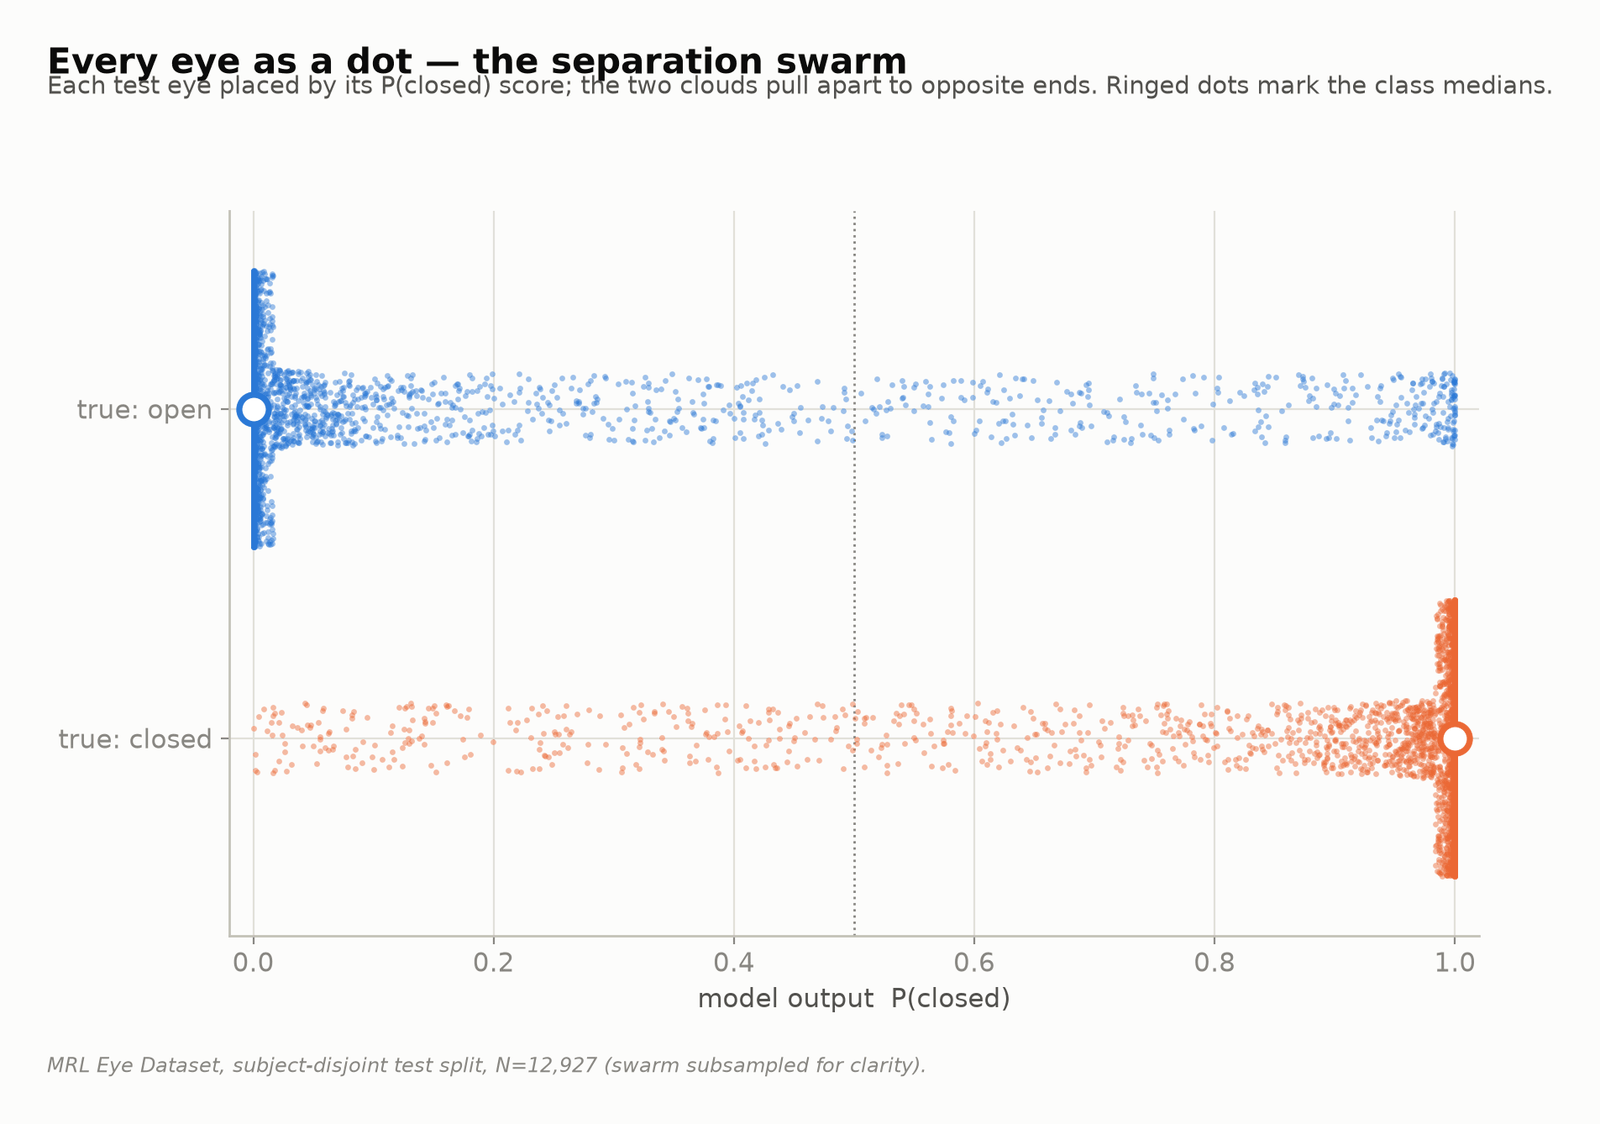
\includegraphics[width=\linewidth]{figures/blink_B1_swarm.png}
\caption{Separation swarm --- every test eye positioned by its predicted probability of the closed state.}
\label{fig:49}
\end{figure}

Two clouds occupy opposite extremes with a sparse interior, the visual form of 0.9836 ROC-AUC. The gap between ranking quality and operating-point accuracy is the actionable quantity:

\begin{equation}
\label{eq:270}
\mathrm{ROC\text{-}AUC} - \mathrm{Acc} = 0.9836 - 0.9367 = 0.0469 ,
\end{equation}

and a classifier ordering this well but scoring materially lower is \emph{misthresholded}, not underpowered. By the probabilistic identity \EQREF{146} the only samples that can change class under any threshold move are those in the overlap region, so the sparse interior also bounds what threshold tuning can recover --- which is why the threshold sweep of \FIGREF{52}, rather than a retraining effort, is the right next step.

\FIGREF{50} accounts for class prevalence.

\begin{figure}[pos=htbp]
\centering
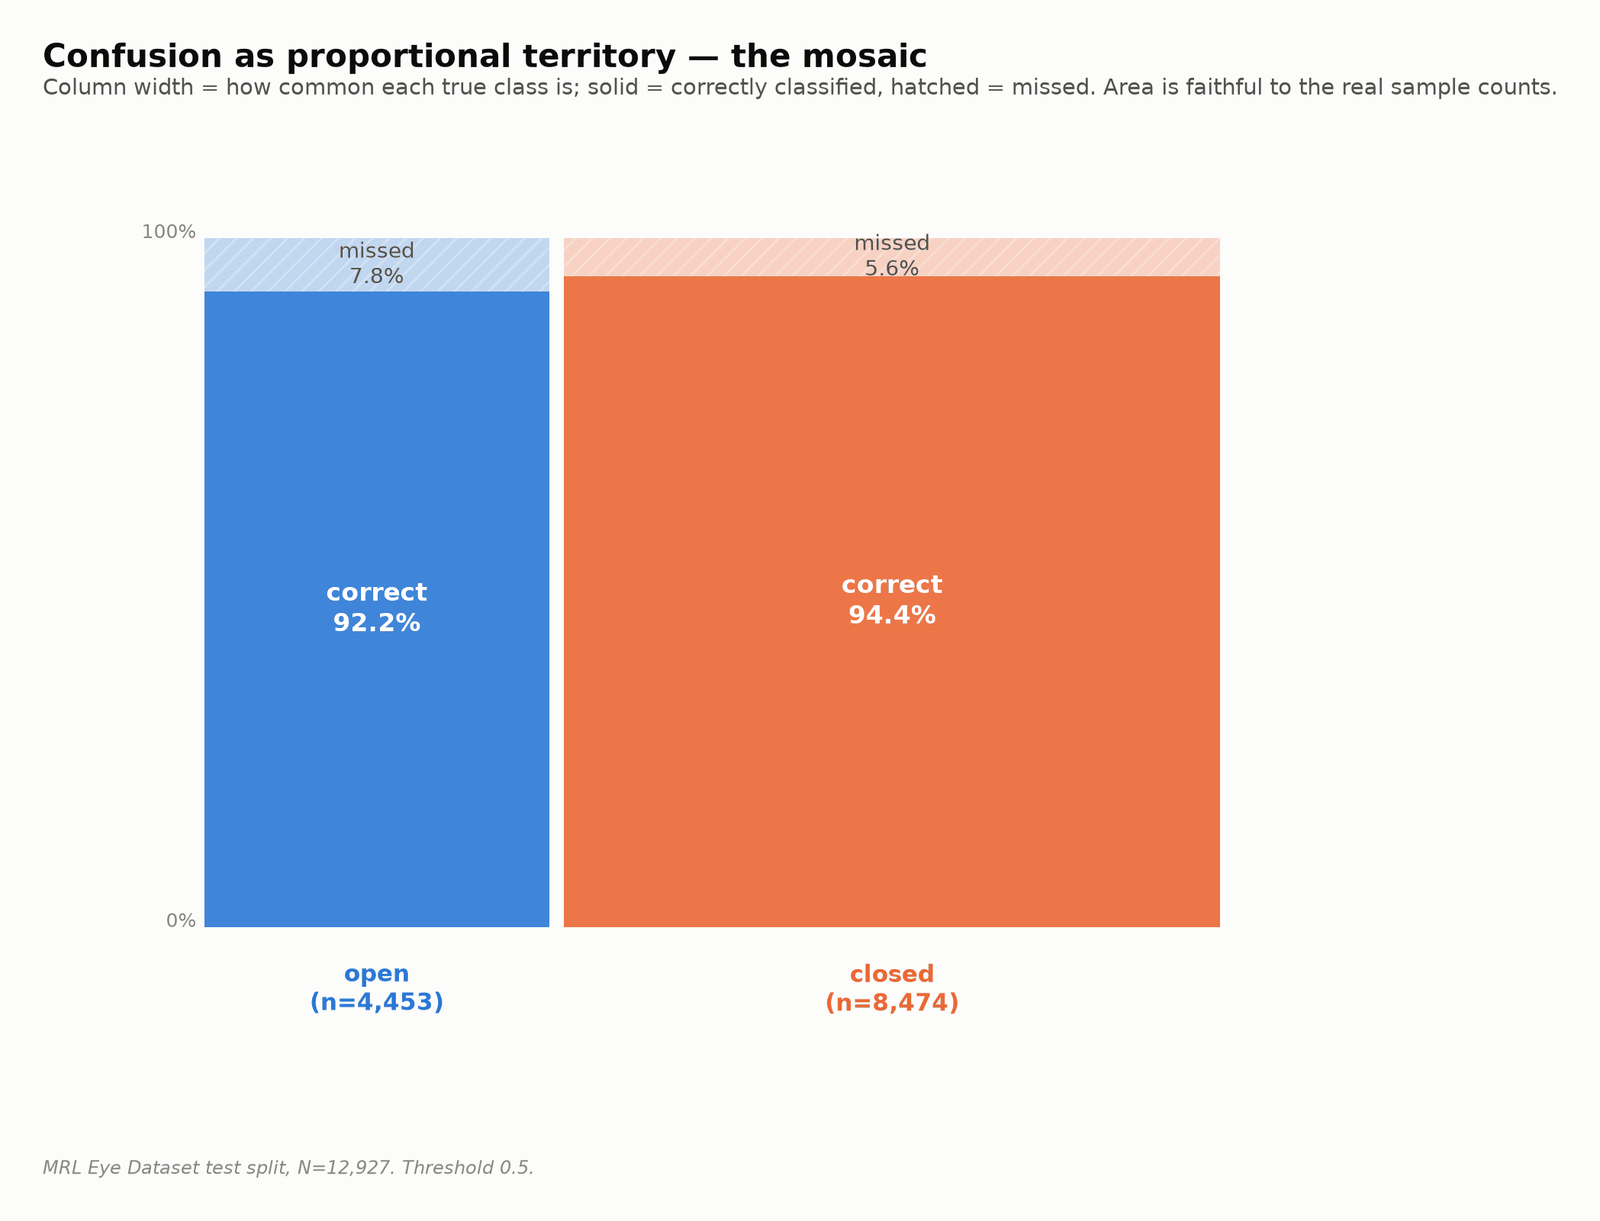
\includegraphics[width=\linewidth]{figures/blink_B2_mosaic.png}
\caption{Confusion mosaic --- territory proportional to class prevalence; column width is prior, solid area is correct classification.}
\label{fig:50}
\end{figure}

At 65.5 \% closed, accuracy is prevalence-weighted toward the majority class, so balanced accuracy \EQREF{141} and MCC \EQREF{144} are the appropriate summaries and both remain high; performance is therefore not a prior artefact. The mosaic exposes the asymmetry governing deployment:

\begin{equation}
\label{eq:271}
\begin{aligned}
\mathrm{FP} = 347 \;\text{open eyes classified closed}\; ( 7.79 \% \;\text{of open} ) , \\
\mathrm{FN} = 471 \;\text{closed eyes classified open}\; ( 5.56 \% \;\text{of closed} ) .
\end{aligned}
\end{equation}

At the frame level these are spurious-click and missed-blink pressure respectively; what the state machine of \ALGREF{5} makes of them is the subject of \FIGREF{52}.

\FIGREF{51} tests probabilistic honesty.

\begin{figure}[pos=htbp]
\centering
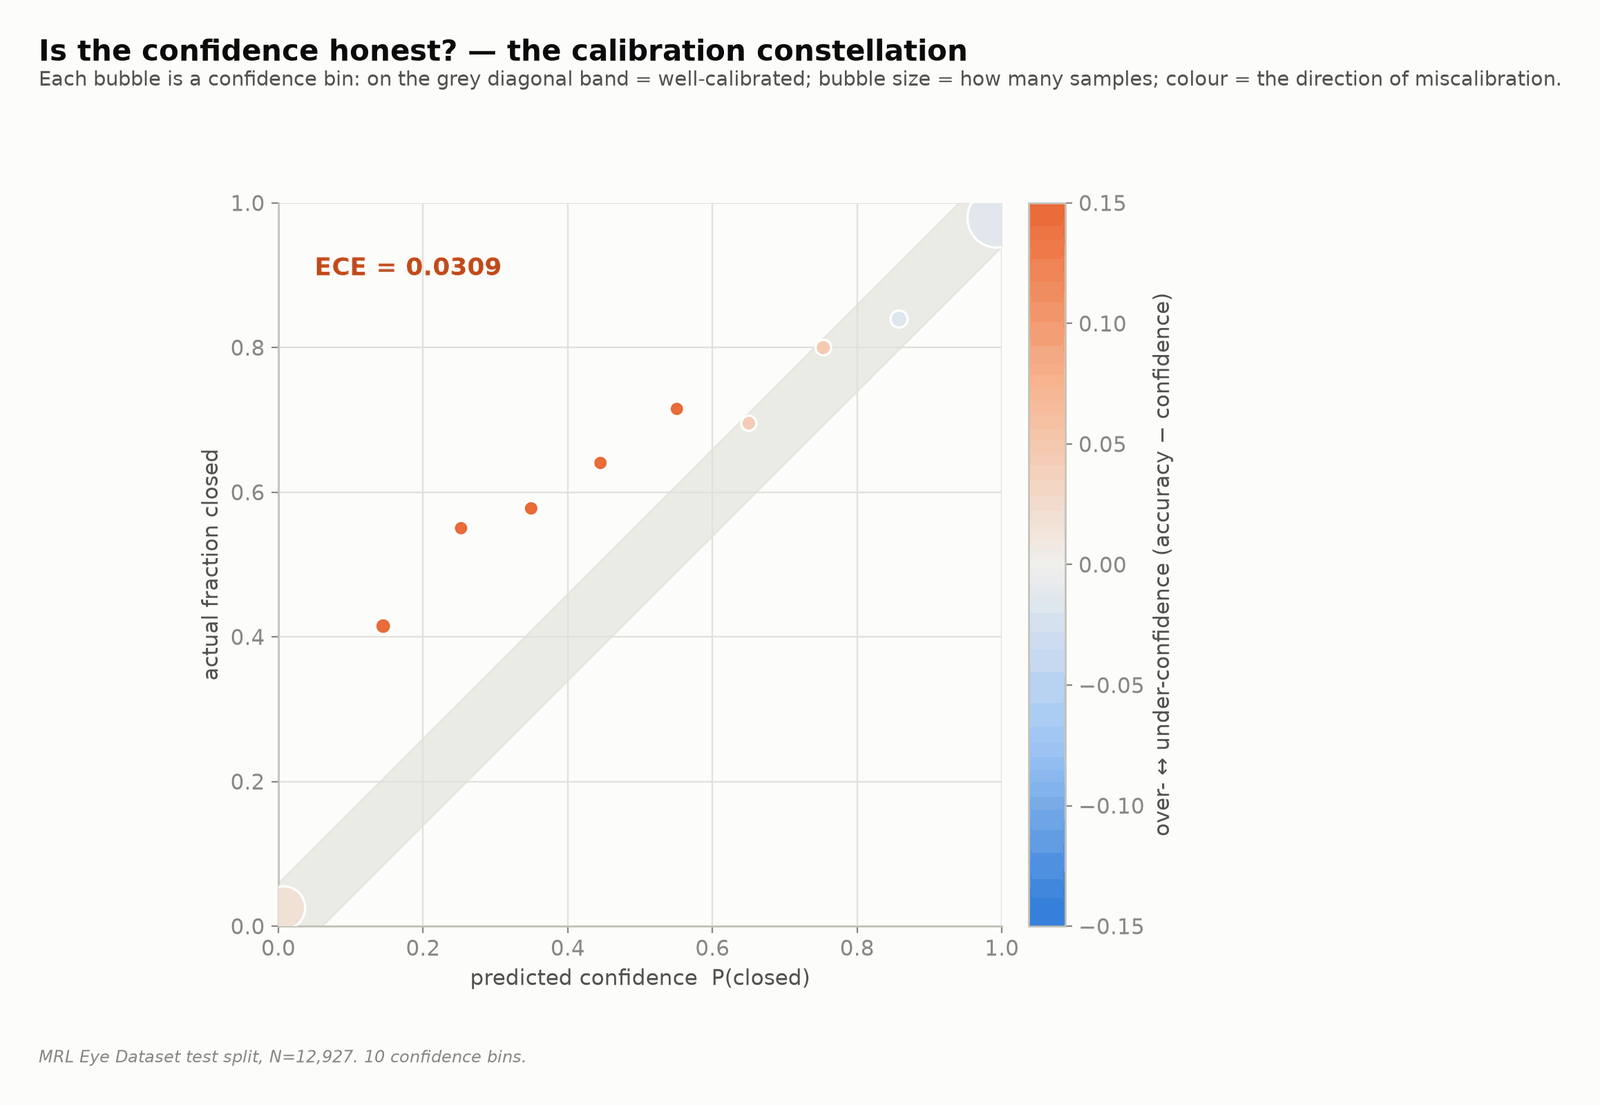
\includegraphics[width=\linewidth]{figures/blink_B3_constellation.png}
\caption{Calibration constellation --- confidence bins as bubbles against observed accuracy.}
\label{fig:51}
\end{figure}

Expected calibration error by \EQREF{150} is

\begin{equation}
\label{eq:272}
\begin{aligned}
\mathrm{ECE} = 2.48 \% , \mathbb{E}[ \text{conf}\; | \;\text{correct} ] = 0.973 , \\
\mathbb{E}[ \text{conf}\; | \;\text{error} ] = 0.785 ,
\end{aligned}
\end{equation}

consistent with the 0.0469 Brier score. The residual miscalibration exceeds the voice network's 1.54 \%, which is expected rather than anomalous: at 136,066 parameters on a binary task with a strong prior, the network sits in the regime where cross-entropy training drives logits toward saturation. Concretely, minimising \EQREF{88} on separable data drives $\|$f$\|$ $\to$ $\infty$ along the max-margin direction, and the induced posterior \EQREF{87} approaches a step function; the deviation from calibration is therefore a predictable consequence of the objective rather than a defect of the fit. Calibration nonetheless remains adequate for the state machine's staged progress readout (\ALGREF{5}, line 11), which reports fractional progress toward each click stage and therefore requires per-frame scores to be commensurable \emph{across} frames rather than merely correctly ordered \emph{within} one.

\FIGREF{52} sweeps the decision threshold --- the single most consequential deployment parameter for this modality.

\begin{figure}[pos=htbp]
\centering
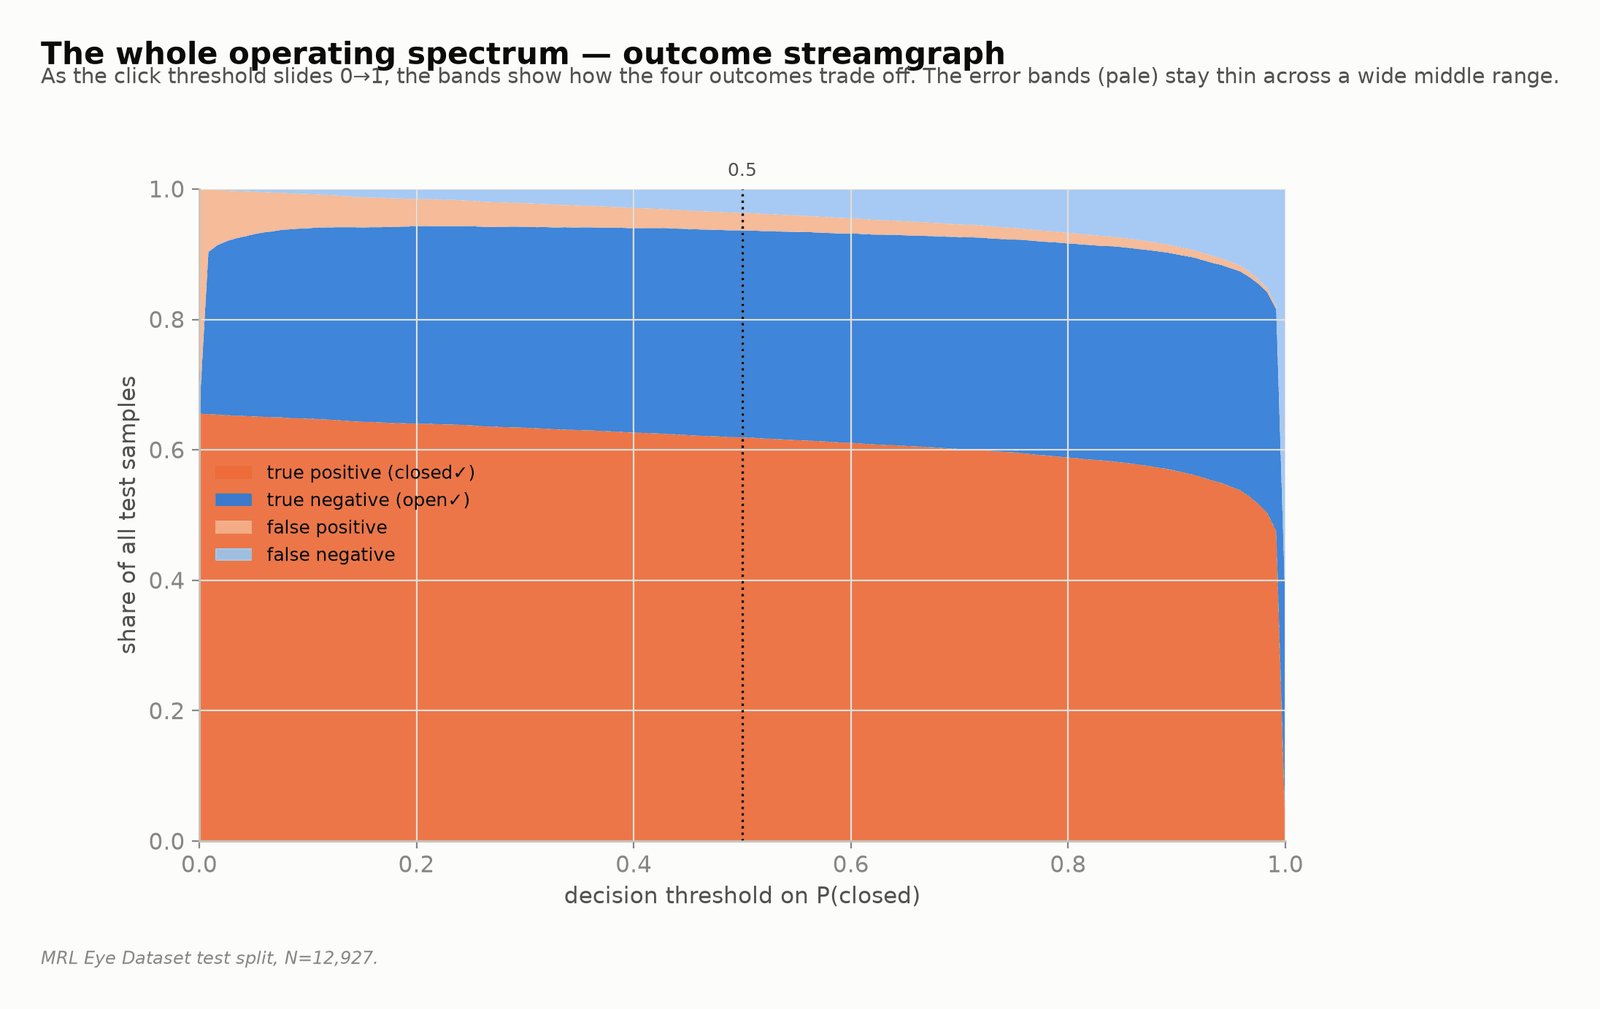
\includegraphics[width=\linewidth]{figures/blink_B4_streamgraph.png}
\caption{Outcome streamgraph --- the four confusion outcomes trading off continuously as the decision threshold slides from 0 to 1.}
\label{fig:52}
\end{figure}

The accuracy-optimal threshold is

\begin{equation}
\label{eq:273}
\begin{aligned}
\zeta _{\mathrm{acc}} = \mathrm{arg\,\mathrm{max}}_{\zeta} \mathrm{Acc}(\zeta ) = 0.212 , \\
\mathrm{Acc}(0.212) = 94.35 \% \mathrm{against} \mathrm{Acc}(0.50) = 93.67 \% ,
\end{aligned}
\end{equation}

and the Youden-optimal threshold \CITE{youden}, weighting both error types equally in rate terms, is

\begin{equation}
\label{eq:274}
\zeta _J = \mathrm{arg\,\mathrm{max}}_{\zeta} [ \mathrm{TPR}(\zeta ) - \mathrm{FPR}(\zeta ) ] = 0.426 .
\end{equation}

Minimising the cost-weighted objective

\begin{equation}
\label{eq:275}
C(\zeta ; w) = w \cdot \mathrm{FP}(\zeta ) + \mathrm{FN}(\zeta )
\end{equation}

for w $\in$ \{3, 5, 10\} gives $\zeta$* = 0.752, 0.845 and 0.955, cutting false positives from 347 to 226, 184 and 114 at the cost of 769, 955 and 1,492 missed blinks. The exchange is strongly non-linear:

\begin{equation}
\label{eq:276}
\Delta \mathrm{FN} / \Delta \mathrm{FP} : 298/121 = 2.46 \;\text{then}\; 186/42 = 4.43 ,
\end{equation}

so each successive false positive removed costs progressively more missed blinks --- the local slope of the receiver-operating curve steepening as the operating point moves into the tail.

\textbf{The cost-weighted reading is the natural one, and for this system it is wrong.} The reason is \EQREF{120}--\EQREF{123}. Because a click requires $n_{\mathrm{run}}$ = 13 consecutive frames above threshold, an isolated false positive cannot fire one; by \EQREF{121} the probability that noise alone manufactures a click from an open eye is

\begin{equation}
\label{eq:277}
\mathrm{FPR}^{n_{\mathrm{run}}} = 0.0779^{13} \approx 3.9 \times 10^{-15} ,
\end{equation}

and the state machine's duration requirement is therefore itself a powerful false-positive filter, with the 100--300 ms natural-blink rejection removing the most common sustained closure as well. A false \emph{negative}, by contrast, breaks a run in progress and silently cancels a click the user deliberately made; by \EQREF{122} the survival probability of a genuine run is

\begin{equation}
\label{eq:278}
( 1 - \mathrm{FNR} )^{n_{\mathrm{run}}} = 0.9444^{13} \approx 0.475 ,
\end{equation}

so under independence more than half of deliberate clicks would be lost. Under the deployed decision rule the asymmetry therefore \textbf{inverts} relative to the frame-level intuition, and thresholds \emph{below} 0.50 are the defensible choice: at $\zeta$ = 0.212 false negatives fall from 471 to 280, raising run survival to

\begin{equation}
\label{eq:279}
( 1 - 280/8474 )^{13} = 0.9670^{13} \approx 0.646 ,
\end{equation}

a 36 \% relative improvement in click retention, while spurious firing rises only to a still-negligible value by \EQREF{277}. The threshold $\zeta$ = 0.212 is thus simultaneously accuracy-optimal by \EQREF{273} and run-integrity-optimal by \EQREF{279}.

This conclusion depends on consecutive-frame errors being less than perfectly correlated. Under the Markov model \EQREF{123} with persistence $\varrho$ the effective run length is $n_{\mathrm{eff}}^{\mathrm{run}}$ = $n_{\mathrm{run}}$(1--$\varrho$)/(1+$\varrho$), and both \EQREF{277} and \EQREF{279} must be recomputed at $n_{\mathrm{eff}}^{\mathrm{run}}$; the \emph{direction} of the asymmetry is preserved for any $\varrho$ < 1, but its magnitude is not. That assumption is not tested here, and a live-session measurement of click precision and recall would be required to confirm it, which Section 6 records as an open item.

\FIGREF{53} shows the same structure as a flow.

\begin{figure}[pos=htbp]
\centering
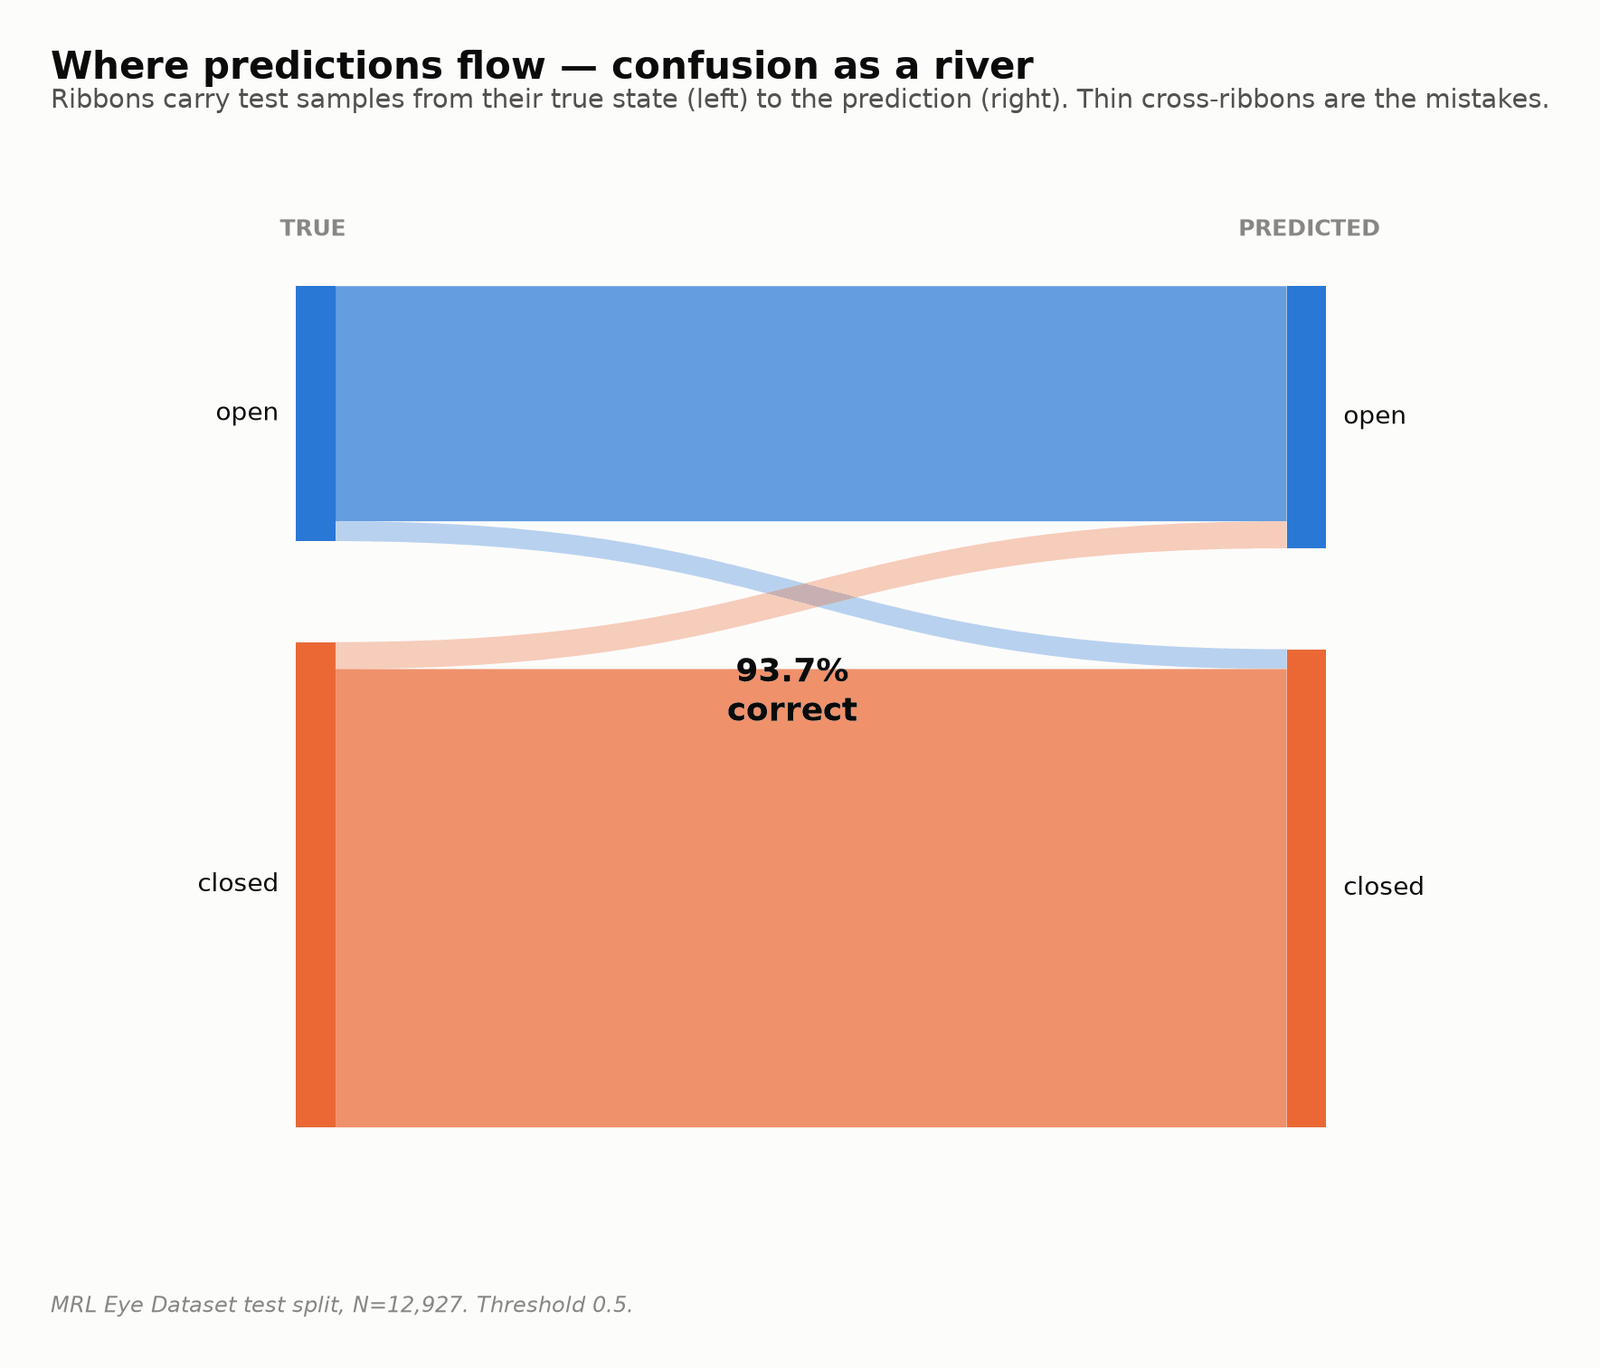
\includegraphics[width=\linewidth]{figures/blink_B5_confusion_flow.png}
\caption{Confusion as a river --- samples flowing from true to predicted state; cross-ribbons are errors.}
\label{fig:53}
\end{figure}

The two cross-ribbons are comparably thick (347 and 471) despite a 2:1 class imbalance, so per-class error \emph{rates} are asymmetric opposite to the prior:

\begin{equation}
\label{eq:280}
\mathrm{FPR} = 347/4453 = 7.79 \% \mathrm{against} \mathrm{FNR} = 471/8474 = 5.56 \% ,
\end{equation}

with per-class F$_{1}$ of 0.909 (open) against 0.951 (closed). This inverts the usual imbalance expectation --- the minority class is usually harder because it is scarcer --- and identifies \textbf{intra-class variance} rather than prior as the governing factor: the open class spans a wide appearance range (gaze direction, illumination, reflective eyewear) while the closed class is comparatively canonical. Formally, if the two classes have equal Bayes-optimal separability but unequal conditional entropy, then

\begin{equation}
\label{eq:281}
H( X | Y = \;\text{open} ) > H( X | Y = \;\text{closed} ) \implies \;\text{error rate}\;_{\mathrm{open}} > \;\text{error rate}\;_{\mathrm{closed}}
\end{equation}

at any fixed capacity. Rebalancing the training prior would therefore not help --- it addresses the wrong term --- whereas enlarging the open-class appearance range would, and eyewear is the specific variation the deployment gap of Section 6 names.

\FIGREF{54} measures score quality independently of any threshold.

\begin{figure}[pos=htbp]
\centering
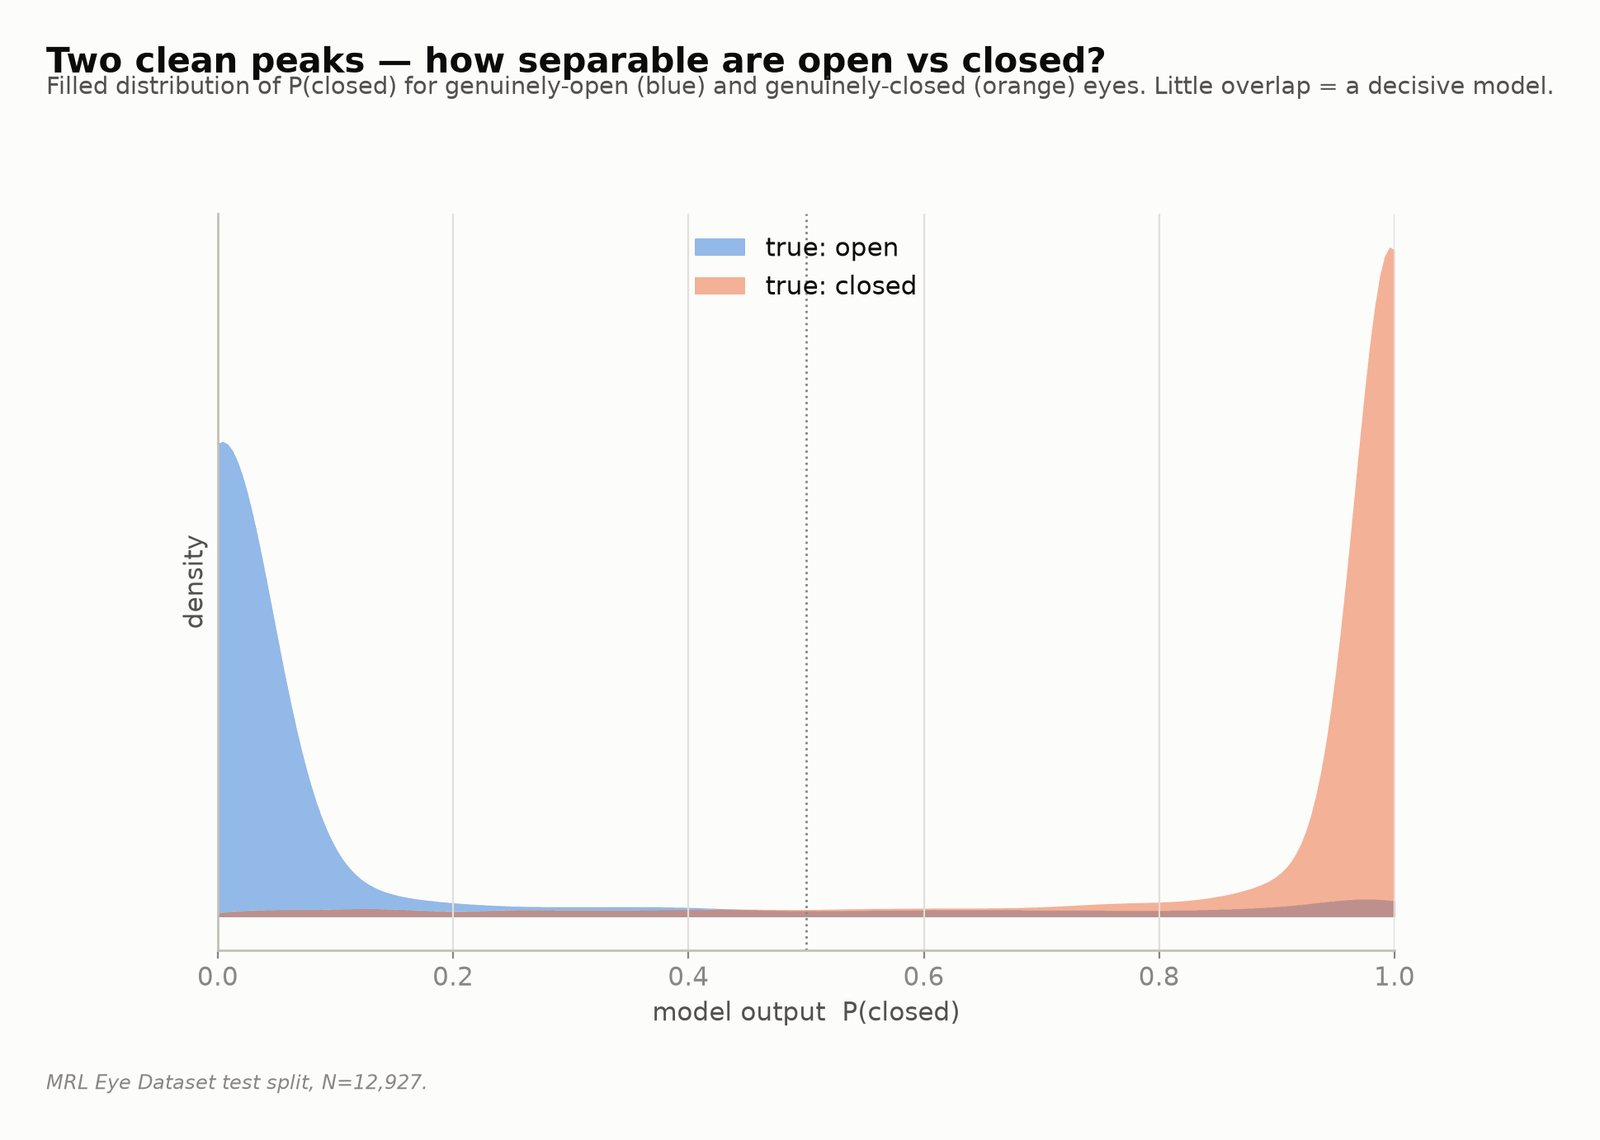
\includegraphics[width=\linewidth]{figures/blink_B6_score_separation.png}
\caption{Score separation --- how cleanly the predicted probability of the closed state divides the two classes.}
\label{fig:54}
\end{figure}

PR-AUC (0.9904) exceeding ROC-AUC (0.9836) is the expected relation on a majority-positive problem \CITE{davis}, since the precision axis is inflated by a high positive prior, and it confirms the ranking is robust under the operative class prior rather than only under a balanced one --- a distinction that matters because the deployed prior, dominated by open eyes during normal use, differs markedly from the test prior of 65.5 \% closed. Separation of this quality places the residual 6.33 \% error in genuinely ambiguous inputs: mid-blink frames where the eyelid is physically part-closed and the binary label is a quantisation of a continuous state. Writing the true eyelid aperture as a latent continuous variable a $\in$ [0,1] with the label y = $\mathbf{1}$[a < a$_{0}$], the conditional Bayes risk near the boundary is

\begin{equation}
\label{eq:282}
\mathbb{P}[ \text{error}\; | a \approx a_{0} ] \to \tfrac{1}{2} ,
\end{equation}

irreducibly, so that component of the error cannot be removed at the per-frame level by any classifier. This is precisely the argument for resolving it temporally, which is what the duration requirement of \EQREF{118} does.

\FIGREF{55} tests whether the network signals its own errors.

\begin{figure}[pos=htbp]
\centering
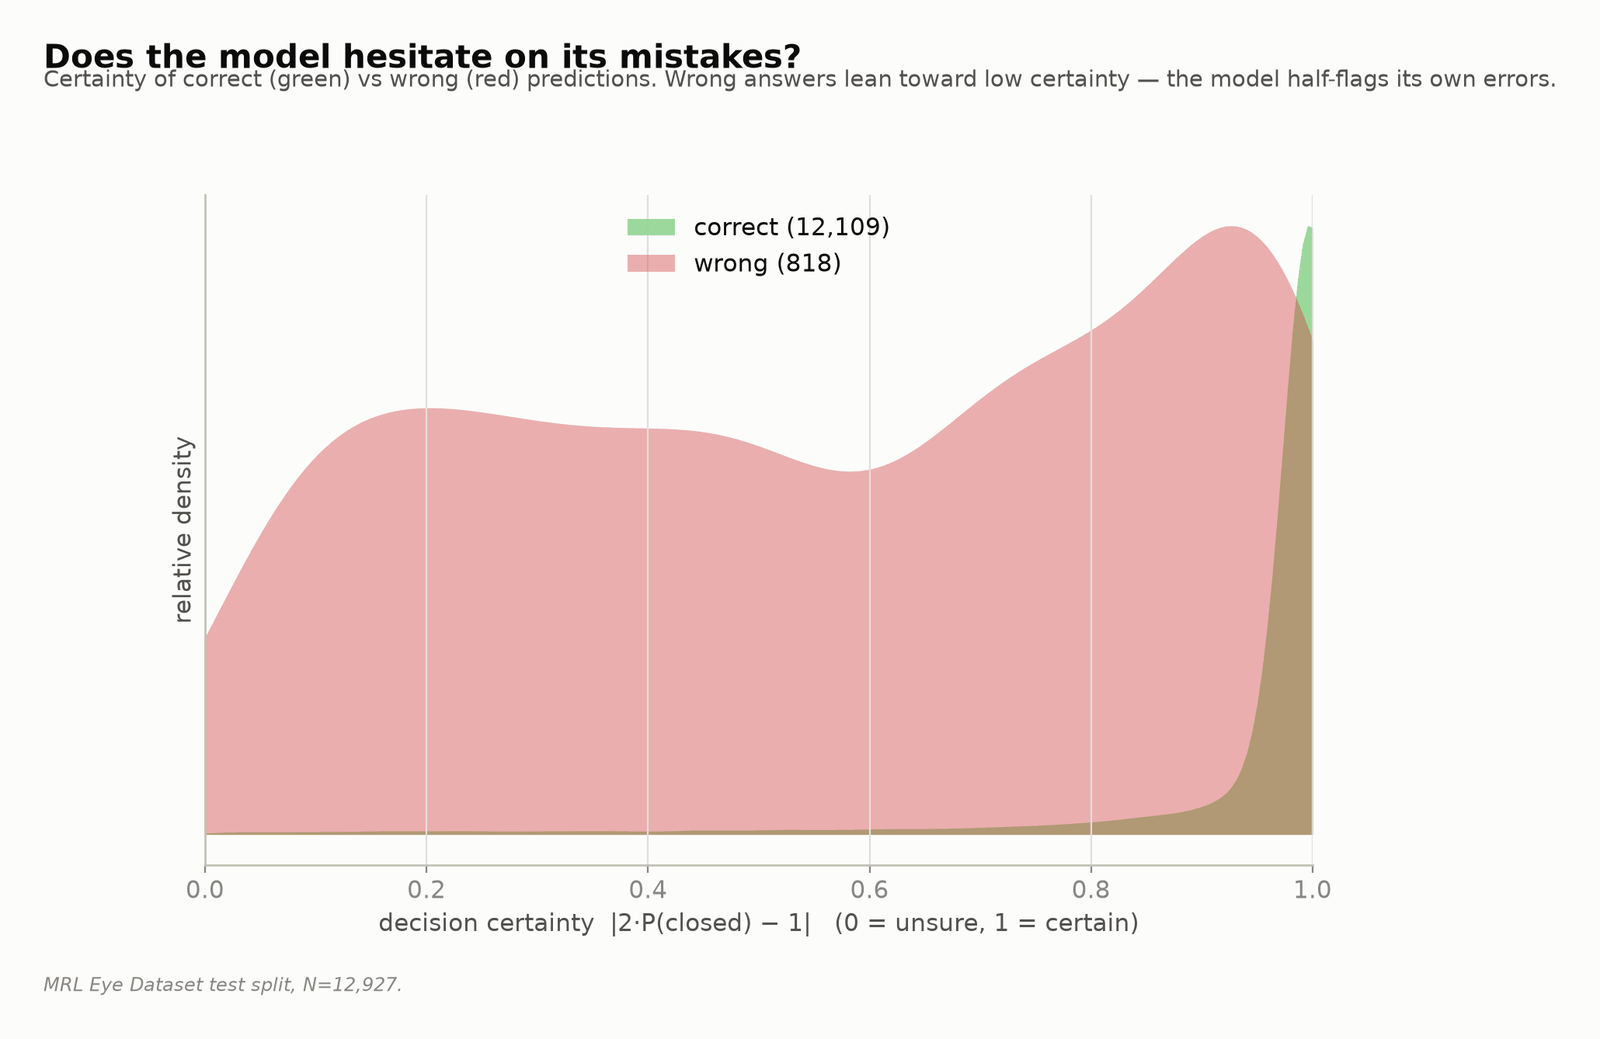
\includegraphics[width=\linewidth]{figures/blink_B7_margin_ridge.png}
\caption{Decision certainty --- the certainty distribution of correct against incorrect predictions.}
\label{fig:55}
\end{figure}

Confidence is a strong but incomplete error detector, AUC 0.9148, and the quintile profile makes the limitation precise. Error rates across confidence quintiles run

\begin{equation}
\label{eq:283}
26.60 \% , 3.95 \% , 0.85 \% , 0.19 \% , 0.04 \% ,
\end{equation}

a spread of

\begin{equation}
\label{eq:284}
26.60 / 0.04 = 665\times
\end{equation}

from lowest to highest. Yet

\begin{equation}
\label{eq:285}
\mathbb{P}[ \text{conf}\; > 0.9 | \;\text{error} ] = 31.2 \% ,
\end{equation}

so roughly one error in three is \emph{confidently wrong} and unreachable by any per-frame gate. This is the quantitative justification for the state machine's duration requirement rather than a confidence threshold: mid-blink ambiguity in the sense of \EQREF{282} is transient while a genuine closure persists, so consecutive-frame agreement suppresses exactly the confident isolated errors that per-frame confidence cannot. Formally, a per-frame gate at level $\zeta_{c}$ reduces error by at most 1 -- $\mathbb{P}$[conf > $\zeta_{c}$ | error], bounded below by 0.312 here, whereas the run requirement suppresses isolated errors at rate governed by \EQREF{277} irrespective of their confidence.

\FIGRANGE{56}{59} re-render the same scores, testing the locality of misordering and the shape of the threshold trade.

\begin{figure}[pos=htbp]
\centering
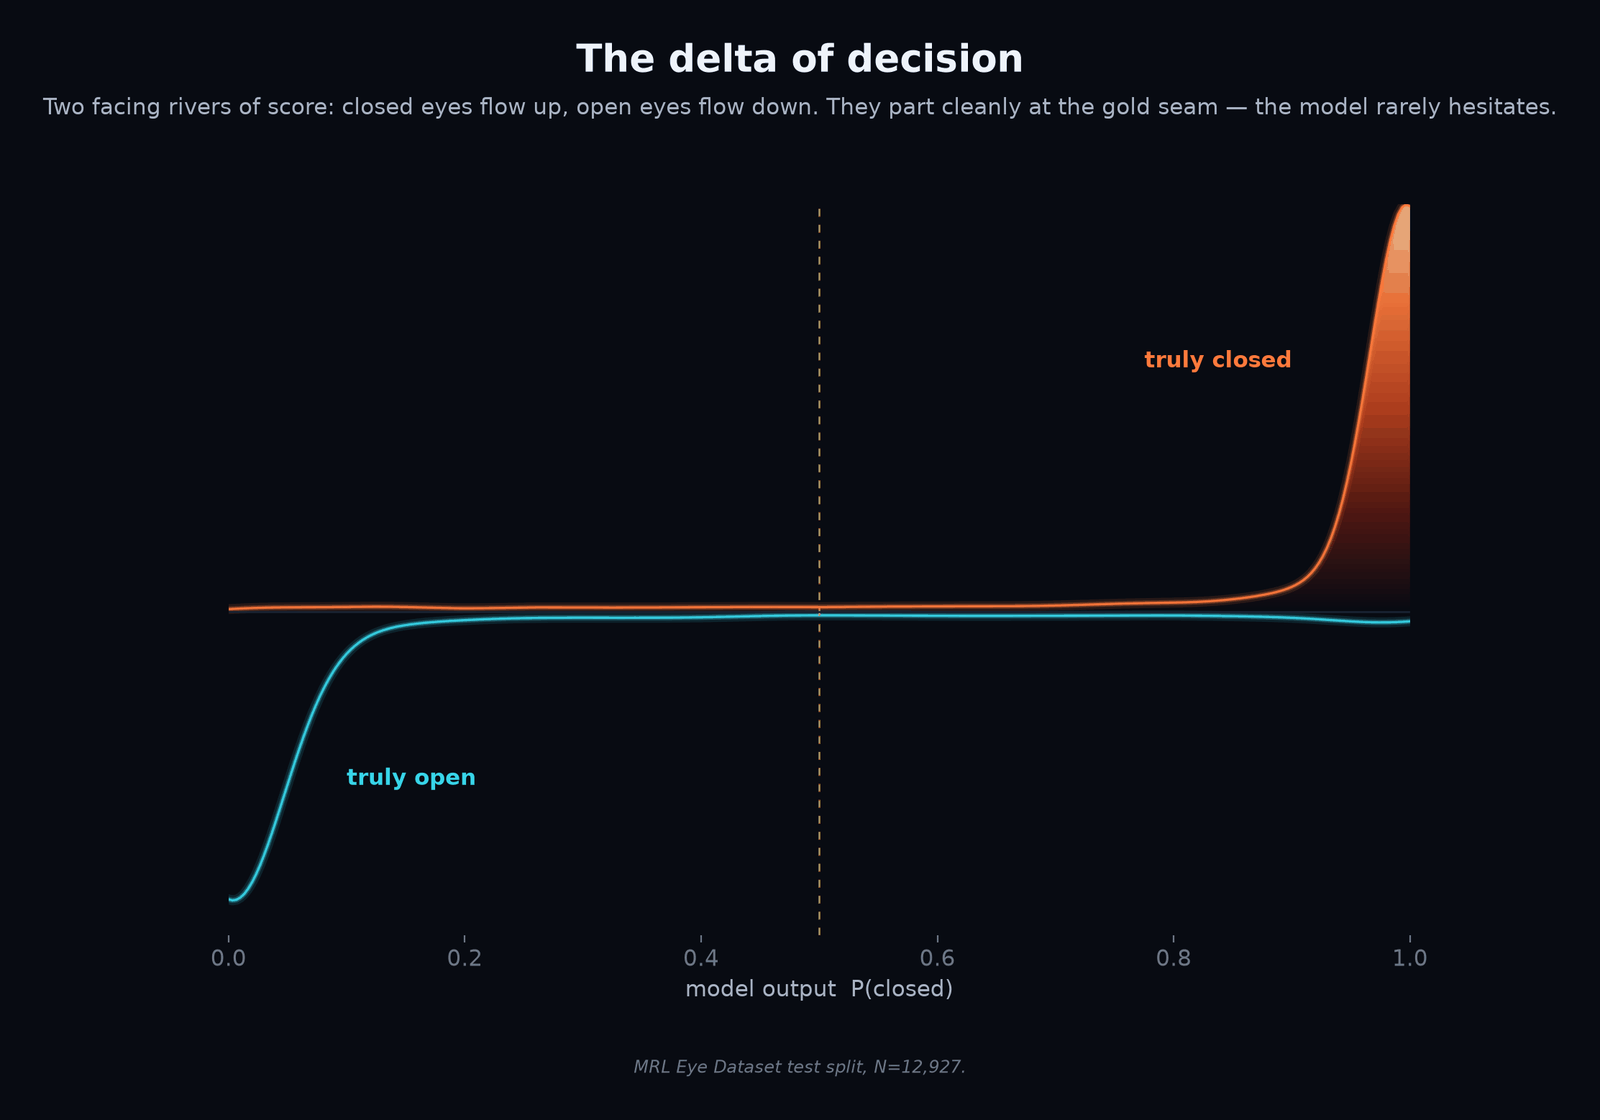
\includegraphics[width=\linewidth]{figures/figures_art_blink_BA1_delta_stream.png}
\caption{The delta of decision --- two facing rivers of predicted score, closed eyes flowing upward and open eyes downward, parting at the decision threshold.}
\label{fig:56}
\end{figure}

The rivers are near-disjoint except at a narrow waist, the geometric expression of 0.9836 ROC-AUC and 0.9904 PR-AUC, and all 6.33 \% of the error lives in that waist --- which is why threshold placement rather than representation is the operative parameter. The asymmetry about the parting line previews the cost analysis: the closed-eye river is the larger (8,474 against 4,453), so shifting the threshold to suppress false clicks sacrifices a disproportionate number of closed-eye detections, which is the non-linear exchange rate measured in \EQREF{276}.

\begin{figure}[pos=htbp]
\centering
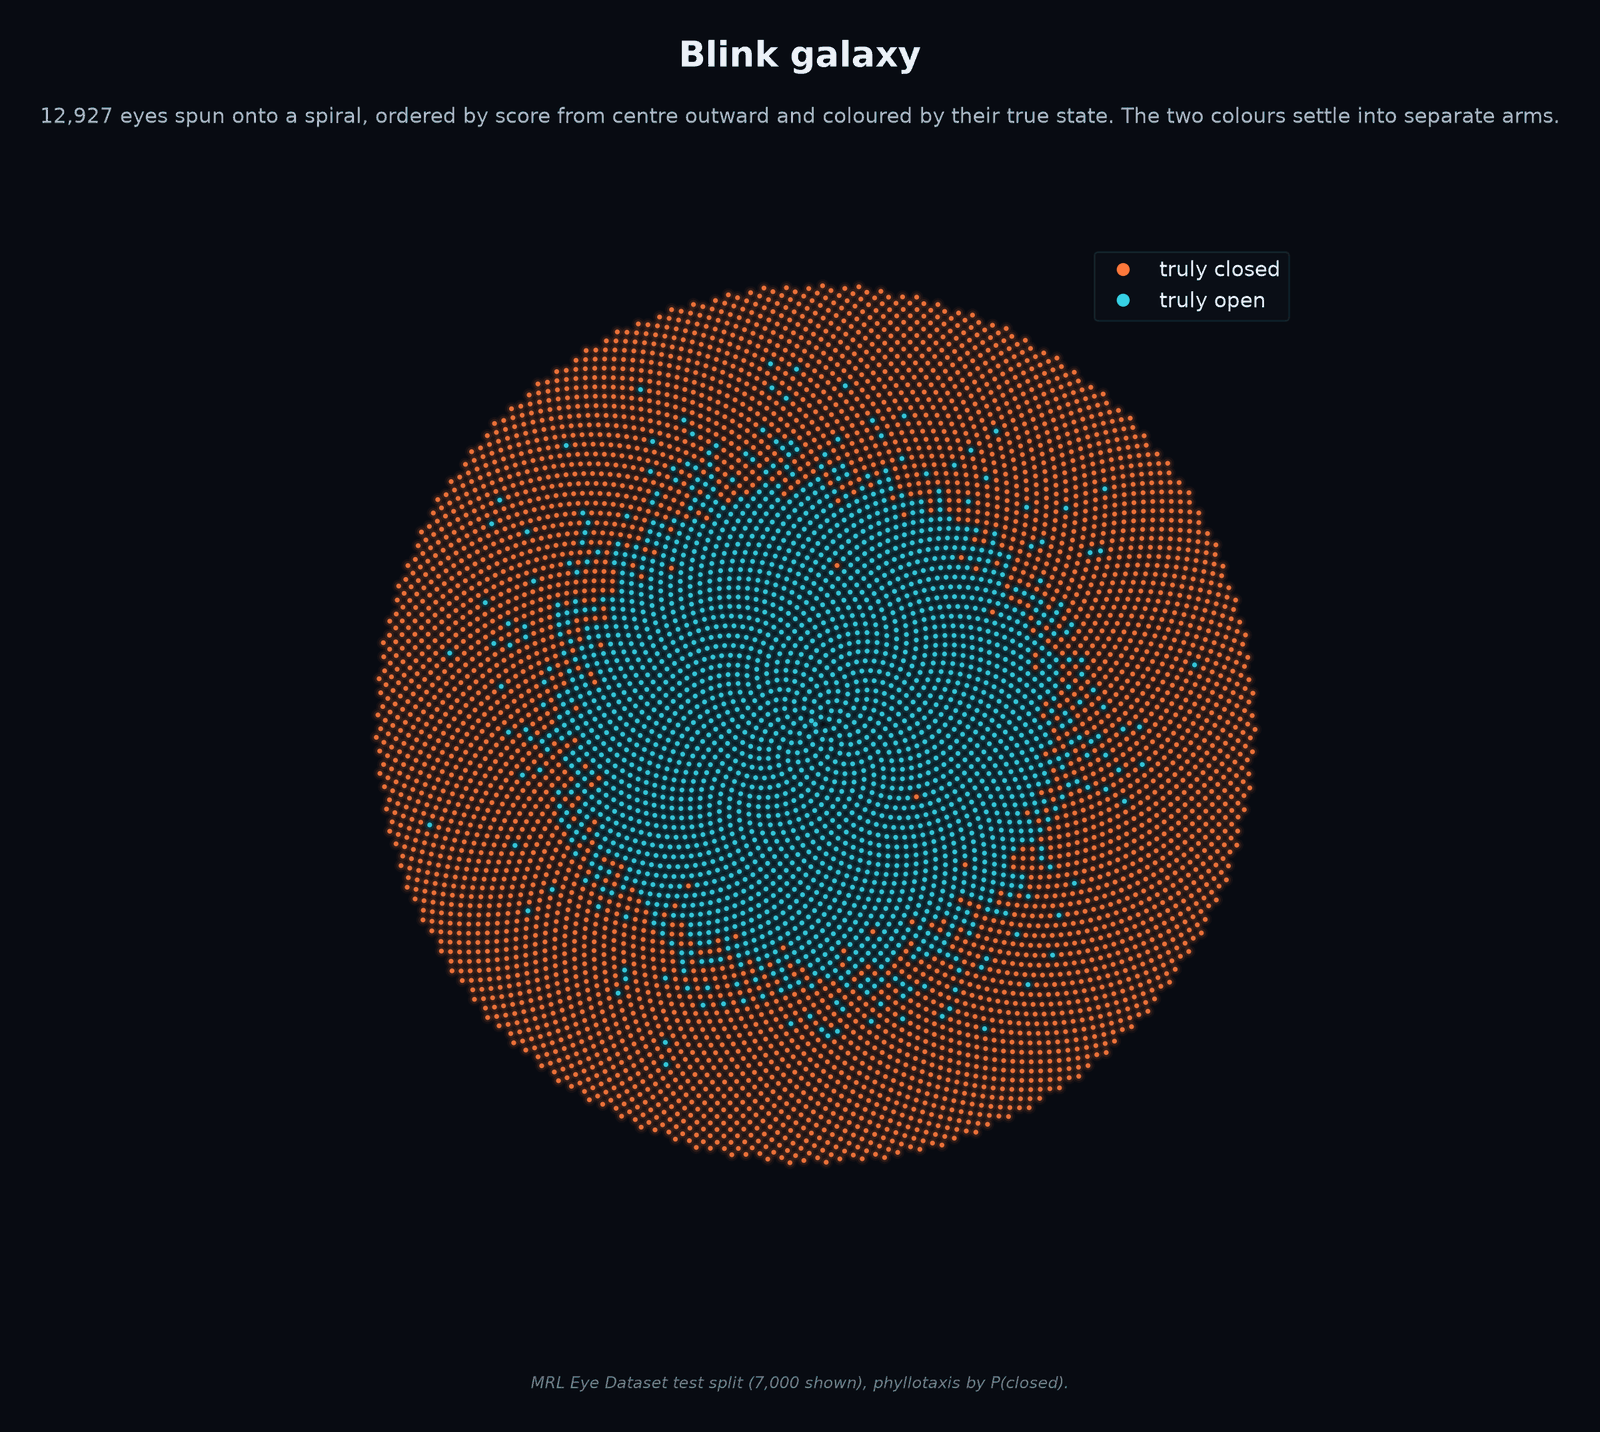
\includegraphics[width=\linewidth]{figures/figures_art_blink_BA2_galaxy.png}
\caption{Blink galaxy --- all 12,927 test eyes arranged on a spiral in order of predicted score and coloured by their true state.}
\label{fig:57}
\end{figure}

Ordering by score and colouring by truth renders ranking quality \emph{countable}. By the identity \EQREF{146}, ROC-AUC is exactly the probability that a randomly chosen closed eye outranks a randomly chosen open one, so contaminated arc length relative to the whole spiral is a direct visual estimate of

\begin{equation}
\label{eq:286}
1 - \mathrm{AUC} = 0.0164 .
\end{equation}

Contamination is confined to a short arc at the crossover rather than distributed along the spiral, establishing that misordering is \textbf{local} --- the precondition for threshold tuning to be effective at all, and therefore the justification for treating \FIGREF{52} as the primary improvement lever. Had misordering been distributed, no threshold would recover the gap \EQREF{270} and retraining would be the only route.

\begin{figure}[pos=htbp]
\centering
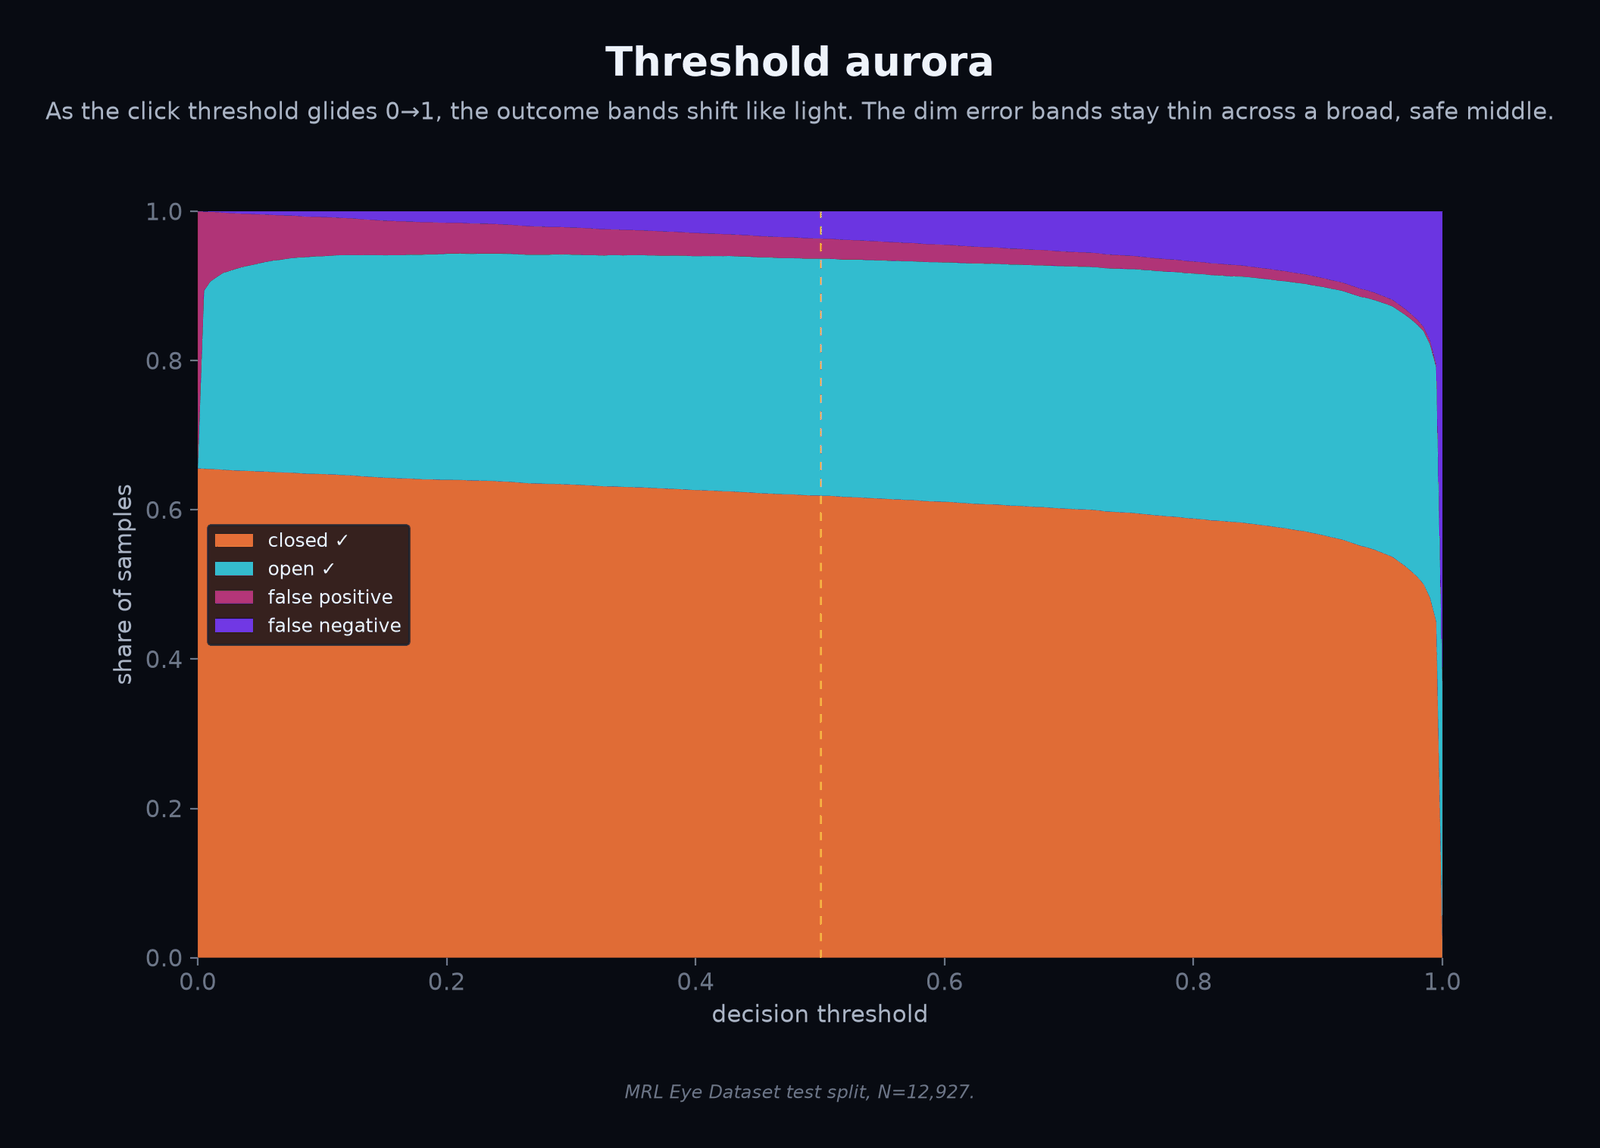
\includegraphics[width=\linewidth]{figures/figures_art_blink_BA3_threshold_aurora.png}
\caption{Threshold aurora --- the four confusion outcomes as continuous bands, as the decision threshold glides from 0 to 1.}
\label{fig:58}
\end{figure}

Continuous rendering exposes gradients the sampled points of \FIGREF{52} cannot. Accuracy peaks at 94.35 \% near $\zeta$ = 0.212 and declines to 93.67 \% at 0.50 while the false-positive band contracts monotonically throughout, so

\begin{equation}
\label{eq:287}
\text{dAcc}\;/d\zeta < 0 \;\text{and dFP}\;/d\zeta < 0 \;\text{simultaneously on}\; \zeta \in [0.212, 1] ,
\end{equation}

meaning the two objectives move in opposite directions with no crossing point and \textbf{no threshold is jointly optimal}. The cost-weighted optima of \EQREF{275} are then read directly off the band gradients. The figure converts an implicit design assumption --- how much worse is a false click than a missed blink --- into an explicit tunable with a measured response curve, which is what allows the conclusion of \EQREF{277}--\EQREF{279} to be revised once the state machine is taken into account rather than argued in the abstract.

\begin{figure}[pos=htbp]
\centering
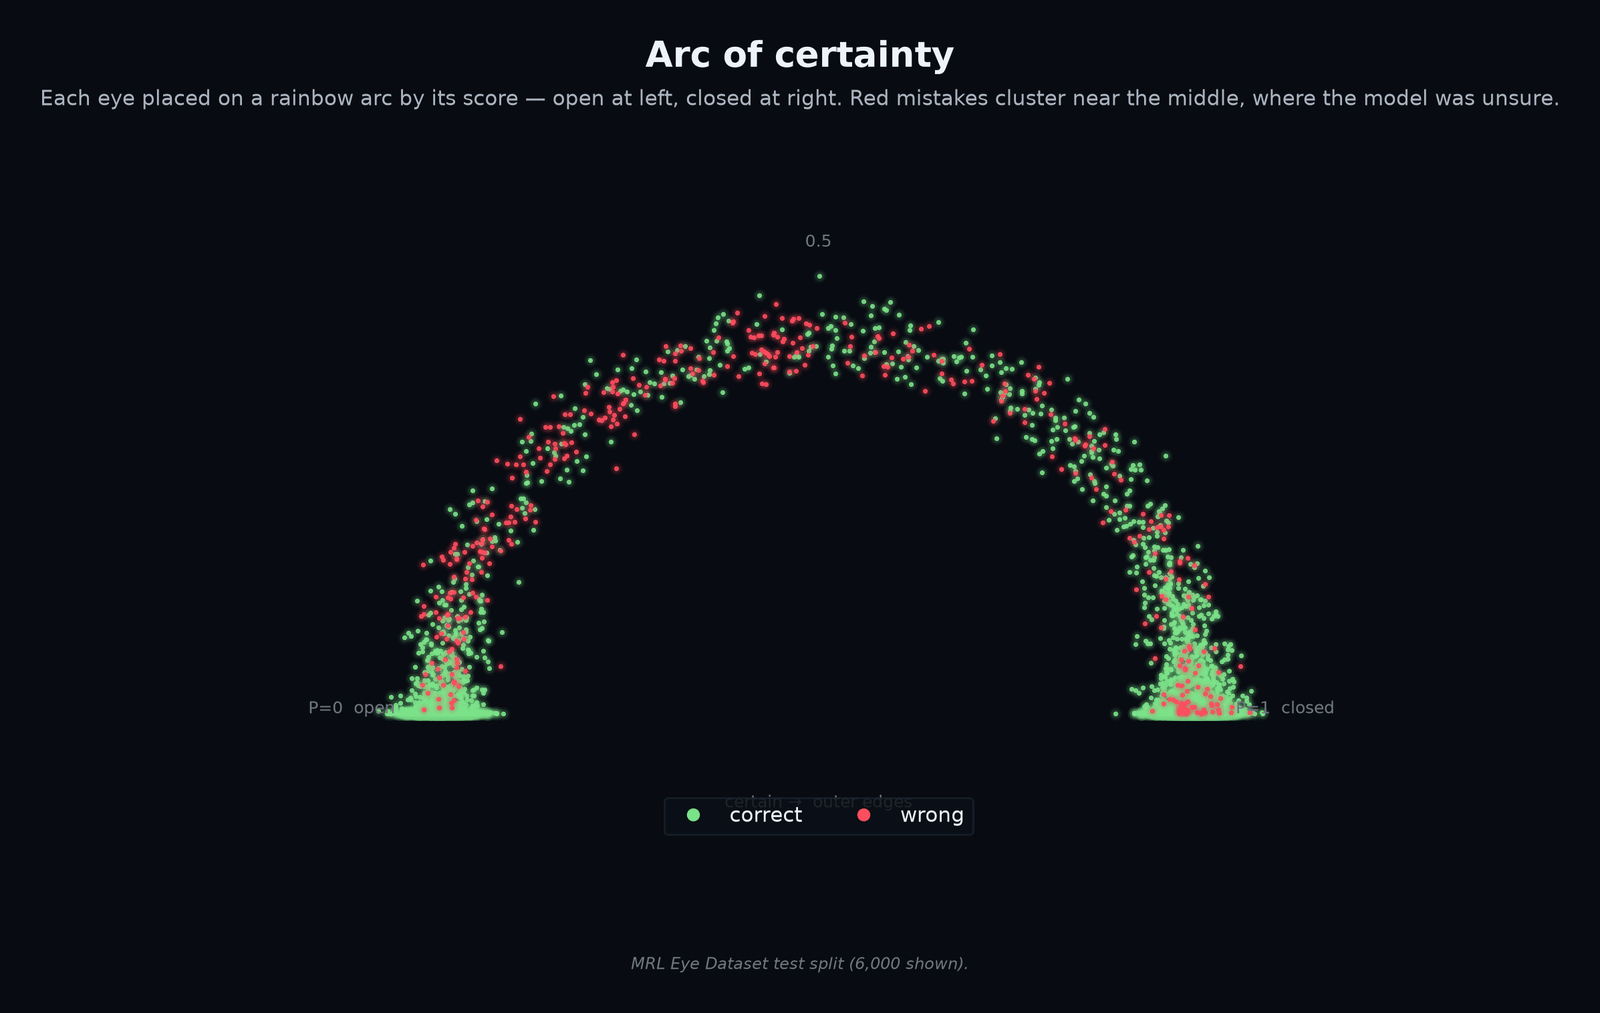
\includegraphics[width=\linewidth]{figures/figures_art_blink_BA4_certainty_arc.png}
\caption{Arc of certainty --- every test eye positioned along an arc by its predicted score, with errors highlighted.}
\label{fig:59}
\end{figure}

Errors concentrate near the arc's centre where certainty is lowest, the basis for uncertainty-aware gating, with error rates falling across quintiles by \EQREF{283}. The counter-population limits the approach: by \EQREF{285}, 31.2 \% of errors sit at the extremes where no gate reaches them. Per-frame uncertainty filtering therefore has a hard floor, and the deployed state machine aggregates across consecutive frames precisely because temporal persistence discriminates where per-frame certainty cannot.

\subsubsection{Why this modality generalises across subjects}

\begin{figure}[pos=htbp]
\centering
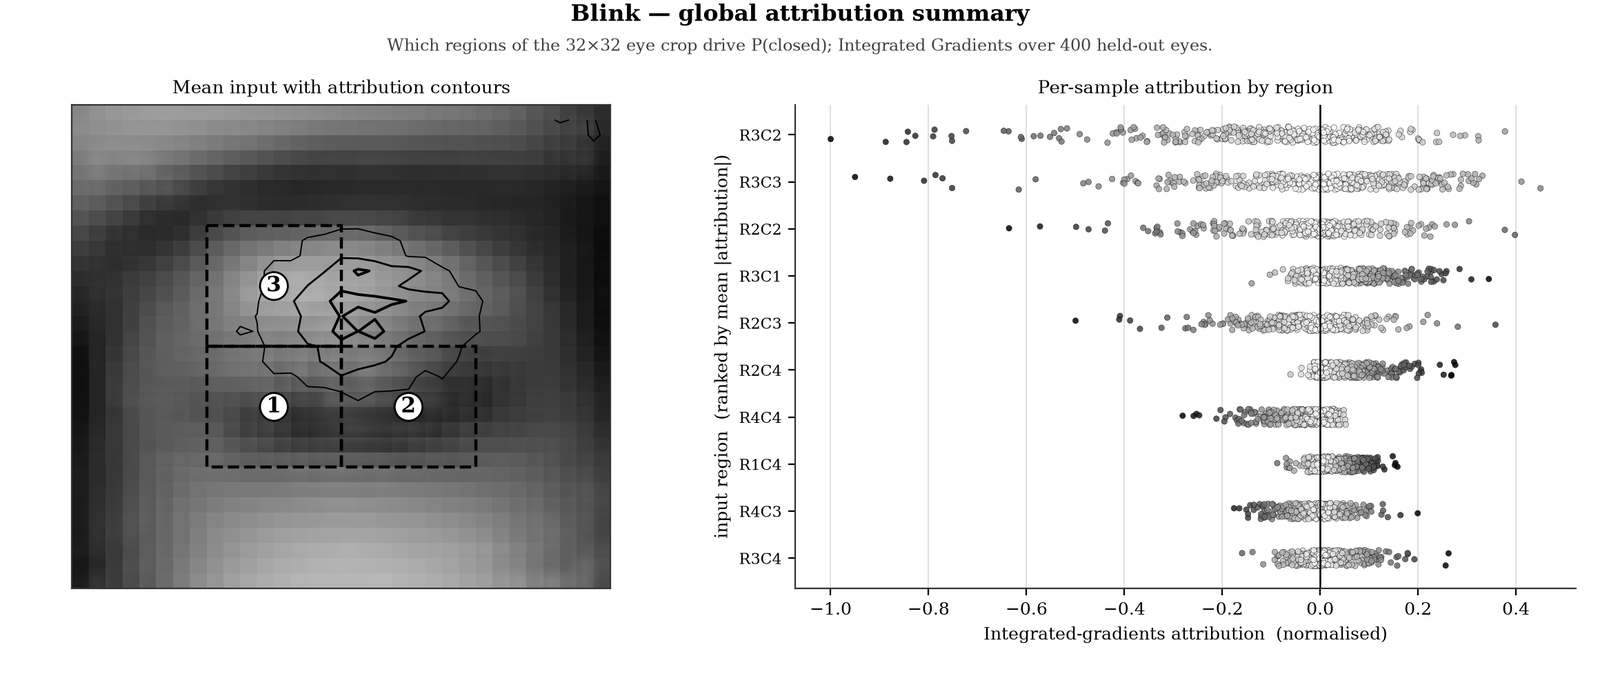
\includegraphics[width=\linewidth]{figures/attribution_blink_A1_summary.png}
\caption{Blink --- global attribution summary: regions of the 32 $\times$ 32 eye crop ranked by mean absolute attribution, with per-sample distributions and the three strongest regions outlined on the mean input.}
\label{fig:60}
\end{figure}

Attribution concentrates in R3C2, R3C3 and R2C2 --- the central and lower-central band containing the palpebral fissure --- while the four corner regions contribute near-zero attribution with tightly clustered per-sample distributions:

\begin{equation}
\label{eq:288}
\begin{aligned}
\Sigma _{k \in \;\text{centre}} | \mathrm{Attr}(R_k) | / \Sigma _k | \mathrm{Attr}(R_k) | \\ 
\gg \\ 
\Sigma _{k \in \;\text{corners}} | \mathrm{Attr}(R_k) | / \Sigma _k | \mathrm{Attr}(R_k) | .
\end{aligned}
\end{equation}

The network located the anatomically correct evidence region without spatial supervision and, more importantly, learned to \emph{ignore} the periphery where hair, spectacle frames and background offer identity-correlated shortcuts. This is the mechanistic basis of its cross-subject robustness: a detector attending only to the fissure is structurally invariant to the appearance factors the leaked-partition evaluation of Section 5.1.1 was silently exploiting. Formally, if the attribution mass on identity-correlated regions is negligible, then the decision function is approximately measurable with respect to the fissure sub-$\sigma$-algebra, and identity enters only through it.

\begin{figure}[pos=htbp]
\centering
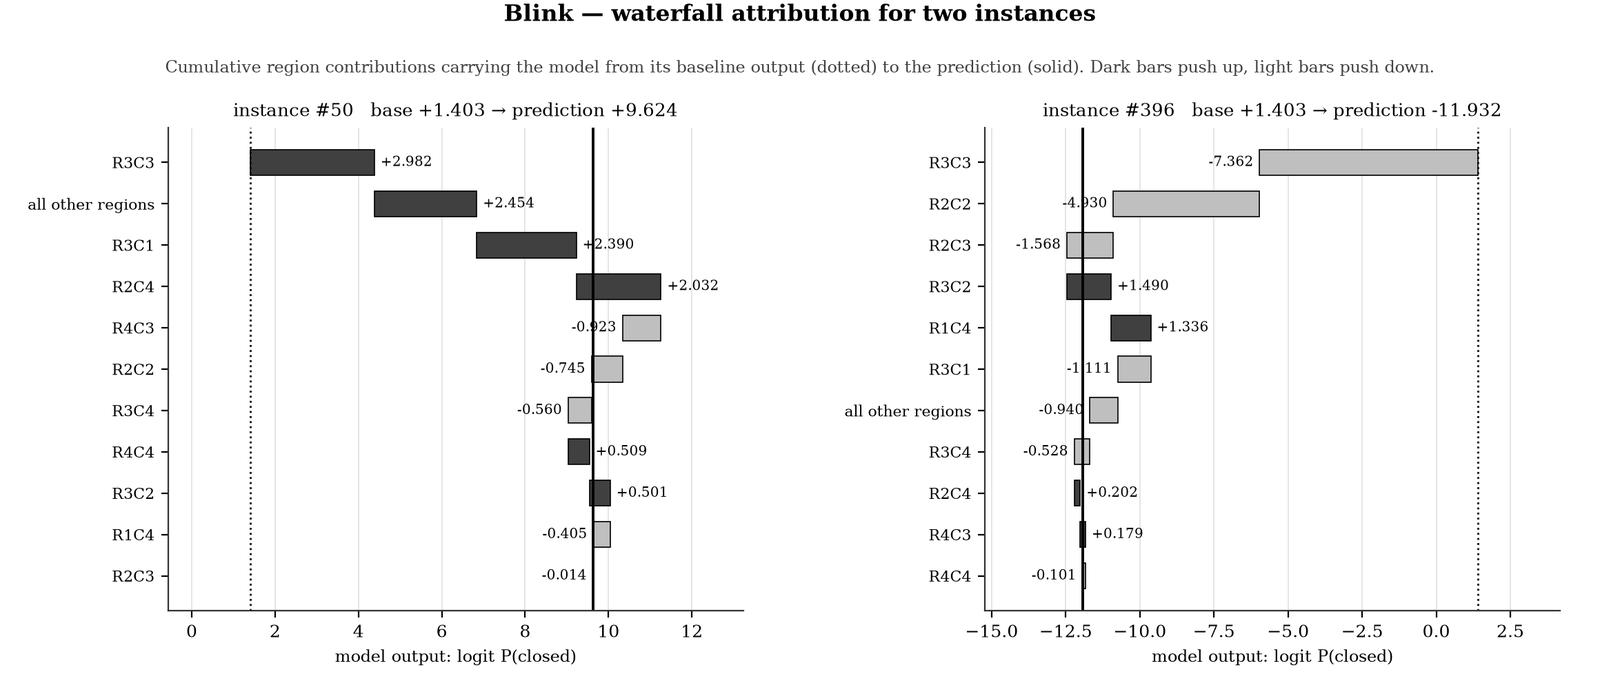
\includegraphics[width=\linewidth]{figures/attribution_blink_A2_waterfall.png}
\caption{Blink --- waterfall attribution for the two most extreme instances, carrying the network from baseline output to prediction region by region.}
\label{fig:61}
\end{figure}

Completeness \EQREF{138} makes this an audit rather than an illustration: the bars sum to the full logit displacement F(x) -- F(0). For both extremes two or three central regions dominate, the remaining thirteen contributing a small alternating-sign residual, so the decision is effectively low-dimensional in region space:

\begin{equation}
\label{eq:289}
\text{effective dimension}\; \approx | { k : |\mathrm{Attr}(R_k)| > 0.1 \cdot \mathrm{max}_j |\mathrm{Attr}(R_j)| } | \approx 3 of 16 .
\end{equation}

This is why 136,066 parameters suffice and why inference costs 0.42 ms --- the capacity requirement is set by the intrinsic dimensionality of the evidence, not by the input dimension, and that is what leaves frame budget for the other three modalities under \EQREF{165}.

\begin{figure}[pos=htbp]
\centering
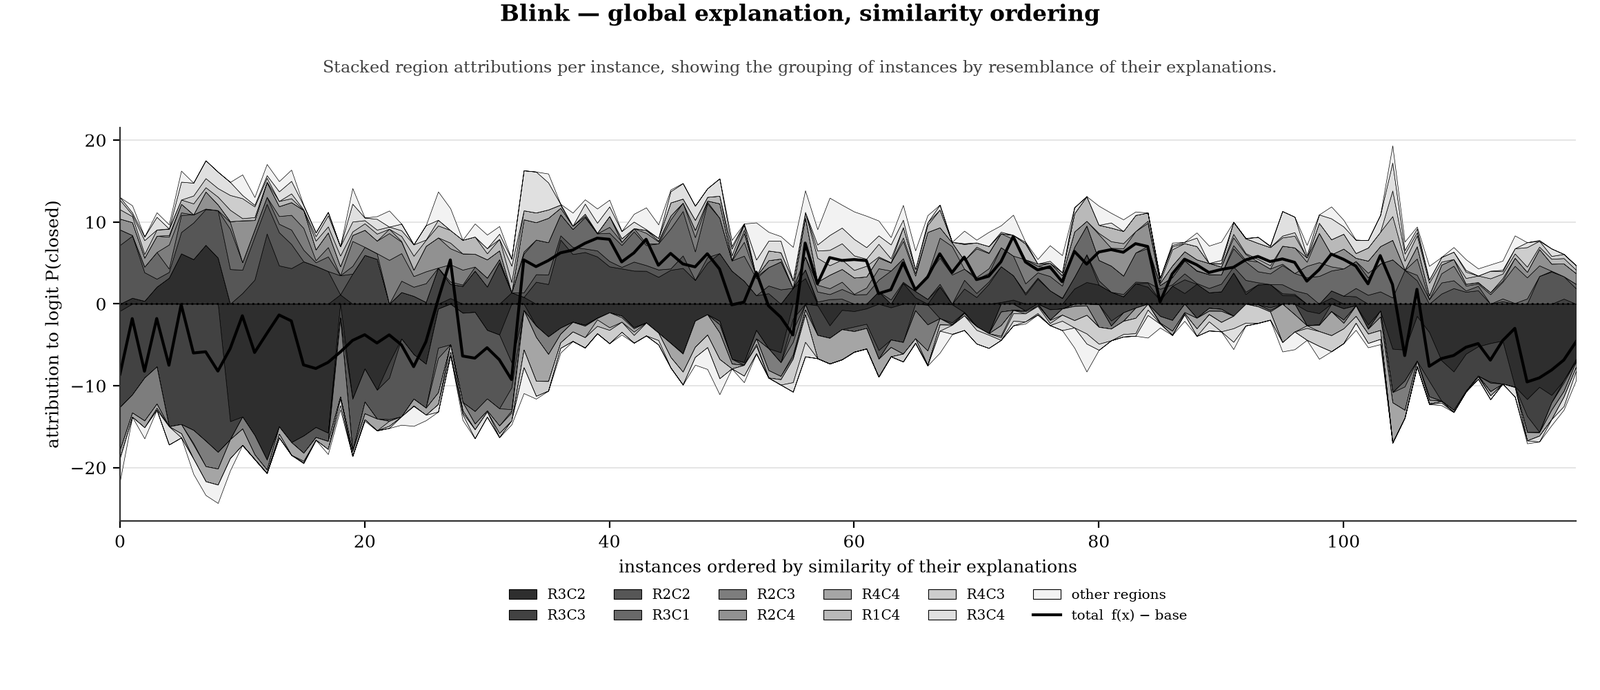
\includegraphics[width=\linewidth]{figures/attribution_blink_A3_similarity.png}
\caption{Blink --- global explanation under similarity ordering: stacked region attributions with instances ordered by resemblance of their explanations.}
\label{fig:62}
\end{figure}

Similarity ordering yields contiguous \textbf{blocks} rather than a gradient, indicating a small number of discrete strategies rather than one continuously varying rule --- the categorical-task structure also seen for voice in \FIGREF{47}, and the opposite of the continua of gaze and head pose. The blocks align with the two classes and, within them, with the \emph{sign pattern} of the central regions, which is evidence that eye state is encoded through the polarity of a localised contrast measurement rather than a distributed template:

\begin{equation}
\label{eq:290}
F_{\mathrm{blink}}(x) \approx w \cdot \mathrm{sgn}( \langle x, \phi _{\mathrm{upper}} \rangle - \langle x, \phi _{\mathrm{lower}} \rangle ) ,
\end{equation}

approximately. A polarity code is cheap to compute and inherently robust to global illumination scaling, since a multiplicative photometric change leaves the sign of a difference unaltered --- consistent with the normalisation \EQREF{15}, with stability across the illumination range present in the corpus, and with the modality's tolerance of the variable lighting a home deployment presents.

\begin{figure}[pos=htbp]
\centering
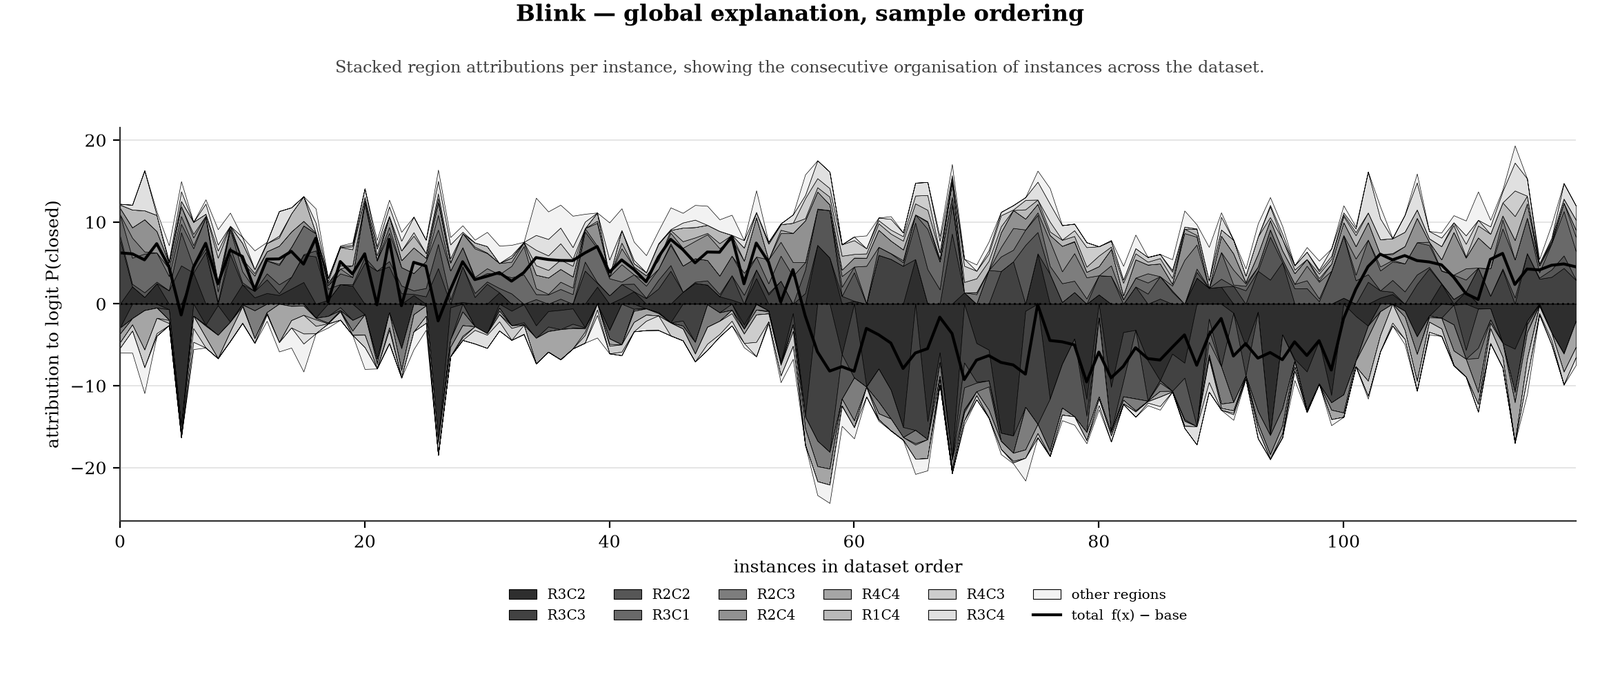
\includegraphics[width=\linewidth]{figures/attribution_blink_A4_ordering.png}
\caption{Blink --- global explanation under dataset ordering: the same stacked attributions with instances in acquisition order.}
\label{fig:63}
\end{figure}

In acquisition order the pattern is stationary, with no drift in region importance across the test sequence. Since the corpus is ordered by subject, stationarity under this ordering is a \textbf{direct test of subject-invariance} of the decision mechanism in the sense of \EQREF{267}, and it passes: the same evidence supports every held-out subject. This is the attribution-level counterpart of group-disjoint evaluation, and it converts 93.67 \% from a number that survived a leakage check into one with an identified invariant mechanism behind it --- the property on which deployment to an unseen user depends.

\FloatBarrier

\subsection{What the four analyses jointly establish}

The four modality sections were deliberately reported in the same order --- headline comparison, mechanism, diagnostic figures, synthesis figures, attribution --- so that their conclusions could be compared rather than merely accumulated. Four findings hold across them.

\subsubsection{One mechanism governs both regression modalities}

The fitted shrinkage gains of \EQREF{191} and \EQREF{225} are

\begin{equation}
\label{eq:291}
\text{gaze}\;: \hat{s} = ( 0.483, 0.481 ) ; \;\text{head pose}\;: \hat{s} = ( 0.822, 0.455, 0.490 ) ,
\end{equation}

placing both networks in the shrinkage regime of \EQREF{155} on every narrow-support axis. That single parameter accounts for:

\begin{itemize}
\item the isotropic radial growth of gaze error (Figs. 4, 13), via the systematic term (1 -- s)$\|\theta\|$ of \EQREF{194}, which has no azimuthal dependence;
\item the constant 2.03--2.21$\times$ head-pose ratio across the pose manifold (\FIGREF{21}), via the multiplicative form \EQREF{211};
\item the axis-ranking inversions between absolute and variance-normalised metrics (Figs. 10, 20), via the competing factors of \EQREF{234};
\item the tolerance convergence of \FIGREF{6}, via the concentration of contraction cost in the tight-tolerance regime;
\item the absence of any localised failure mode in either modality, since \EQREF{194} is a smooth function of $\|\theta\|$ alone.
\end{itemize}

Yaw at $\hat{s}$ = 0.822 is the exception that confirms the account: it is the only wide-support axis, and by the monotonicity \EQREF{227} it is the only one reproduced at near-correct scale. That one measurement replaces what would otherwise be a dozen independent observations is the strongest evidence that the analysis has found the \emph{mechanism} rather than described the \emph{symptoms}.

\subsubsection{The contraction is rational, which redirects the engineering effort}

Inverting the fitted gain raises gaze angular error by 28.5 \% by \EQREF{198}, which by \EQREF{157} establishes that both networks sit near their minimum-MSE shrinkage point s*. Two engineering consequences follow immediately.

First, \textbf{no post-hoc calibration improves them}; only a better representation does, since by \EQREF{156} the risk at the optimum is MSE(s\emph{) = s}$\sigma_{\varepsilon^{2}}$, a quantity that depends only on the representational noise $\sigma_{\varepsilon^{2}}$ and not on any downstream affine transform. This is why Section 5.2.4's identity-count ceiling is decisive rather than merely interesting: it closes the representation route on the available corpus, by \EQREF{222}.

Second, \textbf{the deployed pipeline's structure is correct}. Per-user calibration \EQREF{106} restores scale --- necessarily amplifying noise by the factor 1/$\hat{s}$ $\approx$ 2.07 --- and the temporal filtering \EQREF{112}--\EQREF{117} absorbs the noise that restoration releases. The apparent tension between a calibration stage that amplifies noise and a filter chain that suppresses it is not a design inconsistency but the correct decomposition of the problem, and the analysis identifies it as such.

\subsubsection{The classification modalities are limited by decision logic, not by features}

The complementary diagnosis holds for blink and voice:

\begin{equation}
\label{eq:292}
\begin{aligned}
\mathrm{ROC\text{-}AUC}: 0.9836 (\text{blink}) , \\
0.9961 (\text{voice}) \mathrm{against} \mathrm{Acc}: 93.67 \% , 94.53 \% .
\end{aligned}
\end{equation}

The gaps of 4.69 pp and 5.08 pp place the residual error in \textbf{threshold placement rather than separability}, and both sections demonstrate the consequence directly: a confidence gate lifts voice accuracy to 99.10 \% without changing a weight by \EQREF{255}, and a threshold move lifts blink accuracy to 94.35 \% by \EQREF{273}. The attribution views explain why the features are adequate --- all four networks compute task-appropriate operators:

\begin{itemize}
\item a signed differential across the midline for gaze and head pose, \EQREF{216} and \EQREF{246};
\item a central-fissure contrast polarity for blink, \EQREF{290};
\item a gated high-band spectro-temporal detector for voice, \EQREF{265}.
\end{itemize}

so accuracy rests on identified transferable mechanisms rather than dataset-specific shortcuts. The two categories of limit call for different work, and distinguishing them is the practical payoff of the analysis: capacity for a representation-limited model, decision logic for a threshold-limited one, and the diagnostic \EQREF{292} tells which is which before any effort is spent.

\subsubsection{Fusion with the pretrained baselines is not worthwhile}

A fourth conclusion is negative and applies to both comparable modalities. Per-sample error correlations of

\begin{equation}
\label{eq:293}
r_{\mathrm{AR}} = 0.491 (\text{gaze}) , 0.671 (\text{head pose})
\end{equation}

with oracle-selection bounds \EQREF{163} of 3.303$^{\circ}$ and 3.222$^{\circ}$ give achievable fusion gains of only

\begin{equation}
\label{eq:294}
\text{Gain}\;_{\mathrm{max}} = 8.8 \% (\text{gaze}) , 7.5 \% (\text{head pose}) ,
\end{equation}

which are \emph{upper} bounds requiring an oracle that knows per sample which model is right. The models fail on the same samples, so no gating or ensembling rule can recover the gap, and the cost of a second network --- which by \EQREF{165} would consume a further 2.13 ms or 4.13 ms of a 33.3 ms budget already carrying three networks and a landmark inference --- is not repaid. This removes the most obvious escape route from the recommendation of Section 5.7 and is the reason that recommendation is stated without hedging.

\FloatBarrier

\subsection{Accuracy--efficiency operating point}

Everything above characterises the networks individually. The system-level question is different: whether accuracy of this quality can be obtained inside a budget that lets four modalities run at once on a machine the user already owns. \TABREF{12} reports the trade-off; all latencies are single-thread CPU measurements on the deployed TorchScript modules.

\begin{table}[pos=htbp]
\centering
\caption{Model complexity, footprint and single-thread CPU latency. Ratios are proposed relative to baseline.}
\label{tab:12}
\footnotesize
\begin{tabularx}{\textwidth}{XXXXXX}
\toprule
\textbf{Modality} & \textbf{Model} & \textbf{Parameters} & \textbf{Size (MB)} & \textbf{Latency (ms)} & \textbf{Accuracy relative to baseline} \\
\midrule
Head pose & Proposed & 1,142,339 & 4.60 & 4.13 & 2.12$\times$ higher error \\
Head pose & 6-D rotation baseline & 39,323,398 & 157.32 & --- & --- \\
 & \emph{ratio} & \textbf{*34.4$\times$ fewer}* & \textbf{*34.2$\times$ smaller}* &  &  \\
Voice & Proposed & 101,766 & 0.44 & 2.7 & 0.97 pp lower accuracy \\
Voice & Production ASR engine & --- & 70.90 & 26.5 & --- \\
 & \emph{ratio} &  & \textbf{*161$\times$ smaller}* & \textbf{*9.8$\times$ faster}* &  \\
Blink & Proposed & 136,066 & 0.57 & 0.42 & no neural baseline exists \\
Gaze & Proposed & 551,810 & 2.23 & 2.13 & 1.78$\times$ higher error \\
Gaze & MPIIGaze pre-activation ResNet & 77,533 & 0.31 & --- & --- \\
 & \emph{ratio} & \textbf{*7.1$\times$ more}* & \textbf{*7.2$\times$ larger}* &  & \textbf{*dominated}* \\
\bottomrule
\end{tabularx}
\end{table}

Two qualitatively different outcomes are present and are reported separately rather than averaged into a single verdict.

\subsubsection{Defensible frontier positions: head pose and voice}

For head pose and voice the proposed networks occupy defensible frontier positions. The relevant criterion is whether the accuracy penalty is \emph{sub-linear} in the cost reduction by a wide margin --- the condition for a compact model to be Pareto-relevant rather than merely small. Defining the efficiency elasticity

\begin{equation}
\label{eq:295}
\eta = \mathrm{log}( \text{error ratio} ) / \mathrm{log}( \text{parameter ratio} ) ,
\end{equation}

head pose gives

\begin{equation}
\label{eq:296}
\eta _{\mathrm{pose}} = \mathrm{log}(2.12) / \mathrm{log}(34.4) = 0.751 / 3.538 = 0.212 ,
\end{equation}

so error grows as roughly the fifth root of the parameter reduction. Section 5.3 further showed that the residual error is \emph{absorbed} by the dwell and hysteresis of the gesture rule --- by \EQREF{230}--\EQREF{231} the dwell mean's spread is 2.8$^{\circ}$--4.8$^{\circ}$ against an 18$^{\circ}$ hysteresis band --- rather than reaching the user, so the elasticity understates the deployed advantage.

Voice operates within 0.97 pp of a production ASR engine at 1/161 of its storage and 9.8$\times$ its throughput, on a separate audio thread that does not consume the camera loop's budget at all, though Section 5.4 also showed its risk--coverage curve is markedly worse at matched precision by \EQREF{256} and this is recorded as the substantive gap.

Aggregate vision-pipeline cost is, by \EQREF{165},

\begin{equation}
\label{eq:297}
\begin{aligned}
\tau _{\mathrm{nets}} = 0.42 + 2.13 + 4.13 = 6.68 ms , \\
\;\text{utilisation}\; = 6.68 / 33.3 = 20.1 \% ,
\end{aligned}
\end{equation}

leaving substantial headroom inside the 33.3 ms budget at 30 fps --- headroom that matters because the same loop also runs the shared face-landmark inference, the gesture and blink state machines, and the cursor stabilisation chain. Total deployed footprint across all four modules is, by \EQREF{166},

\begin{equation}
\label{eq:298}
S_{\mathrm{total}} = 7.84 MB ,
\end{equation}

small enough to stay resident in last-level cache on typical consumer processors, which by the arithmetic-intensity argument of \EQREF{167} is disproportionately important on CPU where inference at these sizes is bound by memory traffic rather than arithmetic.

\subsubsection{An unqualified negative result: gaze}

For gaze no such argument survives, and this is recorded as an unqualified negative result. The pretrained baseline is simultaneously

\begin{equation}
\label{eq:299}
\text{more accurate}\; ( 3.621^{\circ} \mathrm{against} 6.439^{\circ} ) \;\text{and smaller}\; ( 77,533 \mathrm{against} 551,810 \;\text{parameters}, 7.1\times \;\text{fewer} ) ,
\end{equation}

dominating on both axes at once. In the Pareto sense there is no operating point at which the proposed gaze network is preferable: for any weighting w $\in$ [0,1] of normalised error against normalised cost,

\begin{equation}
\label{eq:300}
w \cdot \tilde{e}_A + (1-w) \cdot \tilde{c}_A > w \cdot \tilde{e}_R + (1-w) \cdot \tilde{c}_R \;\text{for all w}\; \in [0,1] ,
\end{equation}

since both terms are strictly larger. Section 5.6.4 showed fusion would recover at most 8.8 \%; Section 5.2.4 established the deficit is not closable by augmentation or additional sampling from this corpus. \textbf{The correct engineering decision is to adopt the pretrained model for gaze.}

\subsubsection{The protocol fault changes the decision}

It is worth stating plainly that this conclusion was reachable only because the exposure-disjoint matched per-sample protocol of Section 3.5 made the comparison trustworthy. Under the original protocol the proposed gaze network scored

\begin{equation}
\label{eq:301}
2.84^{\circ} \mathrm{against} \;\text{the pretrained baseline}\;'s \;\text{all}\;-\;\text{participant figure of}\; 2.835^{\circ} ,
\end{equation}

apparently level, and apparently vindicating the decision to train from scratch. Under the corrected protocol the true held-out contrast is

\begin{equation}
\label{eq:302}
6.439^{\circ} \mathrm{against} 3.621^{\circ} ,
\end{equation}

and the baseline is simultaneously 7.1$\times$ smaller. The decision inverts. The magnitude of the illusion is the quantity Theorem 3 decomposes: of the 1.905$^{\circ}$ inflation by \EQREF{171}, between 0.425$^{\circ}$ and 1.068$^{\circ}$ --- 22 \% to 56 \% --- is familiarity rather than difficulty by \EQREF{174}--\EQREF{175}.

A protocol fault that changes an architectural decision is not a bookkeeping matter. We know of no sharper available demonstration that the distinction between a per-pipeline audit and a per-comparison audit has engineering consequences, and it is the reason the audit of Section 3.5 is presented as the principal contribution of this work rather than as a methodological aside.

\FloatBarrier

\subsection{Comparison with existing methods}

\TABREF{13} places the four proposed networks against the baselines they were compared with, and lists the principal published methods on each corpus for context without quoting their figures. That omission is deliberate and is the subject of this paper: figures drawn from the literature were produced under heterogeneous protocols, several of which do not state a grouping key and none of which audits the comparison against its own baseline for exposure asymmetry. Placing such a figure in the same column as ours would assert a comparability that Section 5.1 shows does not hold. The column ``protocol'' therefore carries as much information as the column ``result''.

\begin{table}[pos=htbp]
\centering
\caption{Comparison against the baselines, with published methods listed for context. LOPO = leave-one-person-out; GD = single group-disjoint split; ED = exposure-disjoint comparison stratum (this work). \textbf{Every numeric cell is a measurement made in this study} on the aligned per-sample arrays of Section 4.3; rows whose published figures were not reproduced here are marked \emph{not re-measured} rather than filled with a quoted value, because a figure produced under a different protocol is not the same quantity, and tabulating it beside ours would invite exactly the comparison this paper argues against.}
\label{tab:13}
\footnotesize
\begin{tabularx}{\textwidth}{XXXXXXX}
\toprule
\textbf{Modality} & \textbf{Corpus} & \textbf{Method class} & \textbf{Protocol} & \textbf{Reported result} & \textbf{Params} & \textbf{Cross-model audit} \\
\midrule
Gaze & MPIIGaze & Appearance-based CNN \CITE{mpiigaze} & LOPO (as published) & \emph{not re-measured here} & --- & $\times$ \\
Gaze & MPIIGaze & Pre-activation ResNet \CITE{mpiigaze_pami,preact} & LOPO (as published) & \emph{not re-measured here} & 77,533 & $\times$ \\
Gaze & MPIIGaze & Pre-activation ResNet \CITE{mpiigaze_pami,preact} & \textbf{ED stratum, measured here} & \textbf{3.621$^{\circ}$ angular} (lower bound, EDCP step 5) & 77,533 & \textbf{$\checkmark$ (GERA)} \\
Gaze & MPIIGaze & \textbf{Proposed CNN} & \textbf{GD + ED, measured here} & \textbf{6.439$^{\circ}$ angular} & 551,810 & \textbf{$\checkmark$ (GERA)} \\
Head pose & 300W-LP $\to$ AFLW2000 & Euler-angle CNN \CITE{ruiz} & Corpus-disjoint (as published) & \emph{not re-measured here} & --- & $\times$ \\
Head pose & 300W-LP $\to$ AFLW2000 & 6-D rotation network \CITE{sixdrep} & \textbf{Corpus-disjoint, measured here} & \textbf{3.482$^{\circ}$ MAE} & 39,323,398 & \textbf{$\checkmark$ (negative control)} \\
Head pose & 300W-LP $\to$ AFLW2000 & \textbf{Proposed CNN} & \textbf{Corpus-disjoint + ED, measured here} & \textbf{7.367$^{\circ}$ MAE} & 1,142,339 & \textbf{$\checkmark$ (negative control)} \\
Blink & MRL Eye & Geometric EAR rule \CITE{ear} & n/a (training-free) & not scorable on cropped eyes & 0 & $\times$ \\
Blink & MRL Eye & Proposed CNN, \emph{random row split} & Random row, measured here & 98.17 \% accuracy & 136,066 & n/a \\
Blink & MRL Eye & \textbf{Proposed CNN} & \textbf{GD (subject), measured here} & \textbf{93.67 \% accuracy} & 136,066 & n/a (no baseline) \\
Voice & Speech Commands v2 & Production ASR engine \CITE{vosk,kaldi} & \textbf{Official split, measured here} & \textbf{95.50 \% acc. / 97.43 \% macro-F$_{1}$} & --- & \textbf{$\checkmark$ (risk--coverage)} \\
Voice & Speech Commands v2 & \textbf{Proposed CNN} & \textbf{Official speaker split, measured here} & \textbf{94.53 \% accuracy} & 101,766 & \textbf{$\checkmark$ (risk--coverage)} \\
\bottomrule
\end{tabularx}
\end{table}

Three observations follow, and they are the reason we resist reading \TABREF{13} as a leaderboard.

First, \textbf{the two blink rows are the clearest illustration of the paper's thesis}, and both are our own measurements rather than citations. The identical network scores 98.17 \% under random row splitting and 92.36 \% under subject-disjoint splitting (\TABREF{9}) --- a 5.81 pp difference produced by nothing but the partition, on the same corpus and the same architecture. Any published figure obtained under random row splitting is therefore \emph{not} comparable to the 93.67 \% reported here in the ordinary sense; it is a different quantity, and it does not measure the property an assistive interface requires. That is why no such figure is tabulated beside ours.

Second, \textbf{the gaze rows show the asymmetric-exposure problem in situ}. The pre-activation baseline's $\approx$3.6$^{\circ}$ is its LOPO figure over fifteen participants, and its 3.621$^{\circ}$ here is measured on two held-out participants it \emph{trained on}. By EDCP step 5 the latter is a lower bound on its true cross-person error, so the reported gap of 2.818$^{\circ}$ is conservative with respect to the proposed network. The literature offers no way to tighten this without either the baseline's training partition or a full leave-one-person-out retraining, which is precisely the access problem GERA is designed for.

Third, \textbf{the trades this paper claims rest only on rows measured here}. The proposed head-pose network's 7.367$^{\circ}$ at 1.14 M parameters and the baseline's 3.482$^{\circ}$ at 39.3 M parameters were produced in the same run, on identical crops, from one aligned array set, which is what makes the 34.4$\times$ / 2.12$\times$ trade of \EQREF{296} a real measurement rather than citation arithmetic. Where the table says \emph{not re-measured}, no claim of ours depends on that row.
